\documentclass[
	% -- opções da classe memoir --
	12pt,				% tamanho da fonte
	openright,			% capítulos começam em pág ímpar (insere página vazia caso preciso)
	twoside,			% para impressão em recto e verso. Oposto a oneside
	a4paper,			% tamanho do papel. 
	% -- opções da classe abntex2 --
	%chapter=TITLE,		% títulos de capítulos convertidos em letras maiúsculas
	%section=TITLE,		% títulos de seções convertidos em letras maiúsculas
	%subsection=TITLE,	% títulos de subseções convertidos em letras maiúsculas
	%subsubsection=TITLE,% títulos de subsubseções convertidos em letras maiúsculas
	% -- opções do pacote babel --
	english,			% idioma adicional para hifenização
	brazil%,				% o último idioma é o principal do documento
%	sumario=tradicional
	]{abntex2}

%%%%%%%%%%%%%%%%%%%%%%%%%%%%%%%%%%%%%%
% Fontes
%\usepackage{lmodern}			% Usa a fonte Latin Modern			
%\usepackage[T1]{fontenc}		% Selecao de codigos de fonte.
%\usepackage[utf8]{inputenc}		% Codificacao do documento (conversão automática dos acentos)
%%%%%%%%%%%%%%%%%%%%%%%%%%
\usepackage{fontspec}
\usepackage{polyglossia}
\setmainlanguage{brazil}
\PolyglossiaSetup{brazil}{indentfirst=true}
\setotherlanguages{english}

\setmainfont[Ligatures=TeX]{Latin Modern Roman}
\setsansfont[Ligatures=TeX]{Latin Modern Sans}
\setmonofont{Latin Modern Mono} 
%%%%%%%%%%%%%%%%%%%%%%%%%
% ABNTEX2
\usepackage{lastpage}			% Usado pela Ficha catalográfica
% \usepackage{indentfirst}		% Indenta o primeiro parágrafo de cada seção.
% \usepackage{color}				% Controle das cores
\usepackage{graphicx}			% Inclusão de gráficos
\DeclareGraphicsExtensions{.pdf, .png}
\usepackage{microtype} 			% para melhorias de justificação
%%%%%%%%%%%%%%%%%%%%%%%%%%
% Meus pacotes
% Matemática
\usepackage{csquotes}
\usepackage{amsmath, amsfonts, amssymb}
\usepackage{xfrac}
% Cores
\usepackage{xcolor}
\usepackage{enumitem}
% Tabelas
\usepackage{longtable}
\usepackage{booktabs}
\usepackage{multirow}

%\usepackage{float}
%\floatstyle{plaintop} % tabelas com legenda na parte de cima
%\restylefloat{longtable}  % tabelas com legenda na parte de cima

% Figuras
\usepackage[labelsep=period]{caption} % figuras com subfiguras
\usepackage{subcaption}  % figuras com subfiguras
\graphicspath{{./figuras}}

% Python
\usepackage{minted}

\newcommand{\mM}{mmol.L\textsuperscript{-1}}
\newcommand{\Sal}{Sal\textsuperscript{--}}
\newcommand{\q}{$q$}
% ---
% Pacotes adicionais, usados apenas no âmbito do Modelo Canônico do abnteX2
% ---
\usepackage{lipsum}				% para geração de dummy text
% ---

% ---
% Pacotes de citações
% ---
%\usepackage[brazilian,hyperpageref]{backref}	 % Paginas com as citações na bibl
\usepackage[num]{abntex2cite}	% Citações padrão ABNT
%\usepackage[style=chem-acs, backend=biber,sorting=none,hyperref=true]{biblatex}
%\addbibresource{library.bib}
% --- 
% CONFIGURAÇÕES DE PACOTES
% --- 

%% ---
%% Configurações do pacote backref
%% Usado sem a opção hyperpageref de backref
%\renewcommand{\backrefpagesname}{Citado na(s) página(s):~}
%% Texto padrão antes do número das páginas
%\renewcommand{\backref}{}
%% Define os textos da citação
%\renewcommand*{\backrefalt}[4]{
%	\ifcase #1 %
%		Nenhuma citação no texto.%
%	\or
%		Citado na página #2.%
%	\else
%		Citado #1 vezes nas páginas #2.%
%	\fi}%
%% ---

% ---
% Informações de dados para CAPA e FOLHA DE ROSTO
% ---
\titulo{Estudo estrutural, termodinâmico e cinético sobre a formação e interações de micelas gigantes em sistemas aquosos binários}
\autor{Karl Jan Clinckspoor}
\local{Brasil}
\data{\today}
\orientador{Prof. Dr. Edvaldo Sabadini}
\coorientador{}
\instituicao{%
  Universidade Estadual de Campinas
  \par
  Instituto de Química
  \par
  Programa de Pós-Graduação}
\tipotrabalho{Tese (Doutorado)}
% O preambulo deve conter o tipo do trabalho, o objetivo, 
% o nome da instituição e a área de concentração 
\preambulo{Tese de doutorado realizado no instituto de Química da Unicamp, na área de Físico-Química, que visa estudar micelas gigantes, sua formação, seu crescimento e as interações intermicelares}
% ---


% ---
% Configurações de aparência do PDF final

% alterando o aspecto da cor azul
\definecolor{blue}{RGB}{41,5,195}

% informações do PDF
\makeatletter
\hypersetup{
     	%pagebackref=true,
		pdftitle={\@title}, 
		pdfauthor={\@author},
    	pdfsubject={\imprimirpreambulo},
	    pdfcreator={LaTeX with abnTeX2},
		pdfkeywords={abnt}{latex}{abntex}{abntex2}{trabalho acadêmico}, 
		colorlinks=true,       		% false: boxed links; true: colored links
    	linkcolor=blue,          	% color of internal links
    	citecolor=blue,        		% color of links to bibliography
    	filecolor=magenta,      		% color of file links
		urlcolor=blue,
		bookmarksdepth=4
}
\makeatother
% --- 

% --- 
% Espaçamentos entre linhas e parágrafos 
% --- 

% O tamanho do parágrafo é dado por:
\setlength{\parindent}{1.3cm}

% Controle do espaçamento entre um parágrafo e outro:
\setlength{\parskip}{0.2cm}  % tente também \onelineskip

% ---
% compila o indice
% ---
%\makeindex
% ---

% ----
% Início do documento
% ----
\includeonly{ureia}
\begin{document}

% Retira espaço extra obsoleto entre as frases.
\frenchspacing 

% ----------------------------------------------------------
% ELEMENTOS PRÉ-TEXTUAIS
% ----------------------------------------------------------
% \pretextual

% ---
% Capa
% ---
\imprimircapa
% ---

% ---
% Folha de rosto
% (o * indica que haverá a ficha bibliográfica)
% ---
\imprimirfolhaderosto*
% ---

% ---
% Inserir a ficha bibliografica
% ---

% Isto é um exemplo de Ficha Catalográfica, ou ``Dados internacionais de
% catalogação-na-publicação''. Você pode utilizar este modelo como referência. 
% Porém, provavelmente a biblioteca da sua universidade lhe fornecerá um PDF
% com a ficha catalográfica definitiva após a defesa do trabalho. Quando estiver
% com o documento, salve-o como PDF no diretório do seu projeto e substitua todo
% o conteúdo de implementação deste arquivo pelo comando abaixo:
%
% \begin{fichacatalografica}
%     \includepdf{fig_ficha_catalografica.pdf}
% \end{fichacatalografica}

\begin{fichacatalografica}
	\sffamily
	\vspace*{\fill}					% Posição vertical
	\begin{center}					% Minipage Centralizado
	\fbox{\begin{minipage}[c][8cm]{13.5cm}		% Largura
	\small
	\imprimirautor
	%Sobrenome, Nome do autor
	
	\hspace{0.5cm} \imprimirtitulo  / \imprimirautor. --
	\imprimirlocal, \imprimirdata-
	
	\hspace{0.5cm} \pageref{LastPage} p. : il. (algumas color.) ; 30 cm.\\
	
	\hspace{0.5cm} \imprimirorientadorRotulo~\imprimirorientador\\
	
	\hspace{0.5cm}
	\parbox[t]{\textwidth}{\imprimirtipotrabalho~--~\imprimirinstituicao,
	\imprimirdata.}\\
	
	\hspace{0.5cm}
		1. Palavra-chave1.
		2. Palavra-chave2.
		2. Palavra-chave3.
		I. Orientador.
		II. Universidade xxx.
		III. Faculdade de xxx.
		IV. Título 			
	\end{minipage}}
	\end{center}
\end{fichacatalografica}
% ---

% ---
% Inserir errata
%% ---
%\begin{errata}
%
%$$ FF_{esfera}(q) = \frac{3\left(\sin{(qR)} - qR\cos{(qR)}\right)}{(qR)^3}^2$$
%
%\begin{minted}[mathescape,
%linenos,
%numbersep=5pt,
%gobble=0,
%frame=lines,
%framesep=2mm,
%breakautoindent=true,
%breakanywhere=true,
%breaklines=true,
%python3=True]{python}
%def sphere_FF(q, R):
%    if R == 0:
%        return 0
%    FF = ((3 * (sin(q * R) - q * R * cos(q * R)) / (q * R) ** 3) ** 2)
%    return FF
%\end{minted}
%\end{errata}
% ---

% ---
% Inserir folha de aprovação
% ---

% Isto é um exemplo de Folha de aprovação, elemento obrigatório da NBR
% 14724/2011 (seção 4.2.1.3). Você pode utilizar este modelo até a aprovação
% do trabalho. Após isso, substitua todo o conteúdo deste arquivo por uma
% imagem da página assinada pela banca com o comando abaixo:
%
% \includepdf{folhadeaprovacao_final.pdf}
%
\begin{folhadeaprovacao}
%
%  \begin{center}
%    {\ABNTEXchapterfont\large\imprimirautor}
%
%    \vspace*{\fill}\vspace*{\fill}
%    \begin{center}
%      \ABNTEXchapterfont\bfseries\Large\imprimirtitulo
%    \end{center}
%    \vspace*{\fill}
%    
%    \hspace{.45\textwidth}
%    \begin{minipage}{.5\textwidth}
%        \imprimirpreambulo
%    \end{minipage}%
%    \vspace*{\fill}
%   \end{center}
%        
%   Trabalho aprovado. \imprimirlocal, 24 de novembro de 2012:
%
%   \assinatura{\textbf{\imprimirorientador} \\ Orientador} 
%   \assinatura{\textbf{Professor} \\ Convidado 1}
%   \assinatura{\textbf{Professor} \\ Convidado 2}
%   \assinatura{\textbf{Professor} \\ Convidado 3}
%   \assinatura{\textbf{Professor} \\ Convidado 4}
%      
%   \begin{center}
%    \vspace*{0.5cm}
%    {\large\imprimirlocal}
%    \par
%    {\large\imprimirdata}
%    \vspace*{1cm}
%  \end{center}
  
\end{folhadeaprovacao}
% ---

% ---
% Dedicatória
% ---
\begin{dedicatoria}
   \vspace*{\fill}
   \centering
   \noindent
   \textit{ Este trabalho é dedicado às crianças adultas que,\\
   quando pequenas, sonharam em se tornar cientistas.} \vspace*{\fill}
\end{dedicatoria}
% ---

% ---
% Agradecimentos
% ---
\begin{agradecimentos}

Agradeço à minha mãe, a quem amo muito, por ter sempre me apoiado em toda minha vida. Agradeço à Karen, minha maravilhosa namorada, por todos os singelos momentos vividos até agora. Agradeço à Lia, por ter sido uma ótima companhia, desde o início da graduação.

Agradeço ao Prof. Edvaldo, que dirigiu e focou minha, por vezes dispersa, atenção, e me apoiou nas diversas decisões que eu tive que tomar durante minha pós graduação. Agradeço ao Prof. Jan Skov Pedersen, por ter aceitado me receber em seu laboratório por um mês, mesmo eu sendo um completo amador em sua área de especialização.

Agradeço aos colegas do laboratório B145, pelas discussões e companhia durante esses anos.

Agradeço ao CNPq pelo financiamento.

\end{agradecimentos}
% ---

% ---
% Epígrafe
% ---
\begin{epigrafe}
    \vspace*{\fill}
	\begin{flushright}
		\textit{``Não vos amoldeis às estruturas deste mundo, \\
		mas transformai-vos pela renovação da mente, \\
		a fim de distinguir qual é a vontade de Deus: \\
		o que é bom, o que Lhe é agradável, o que é perfeito.\\
		(Bíblia Sagrada, Romanos 12, 2)}
	\end{flushright}
\end{epigrafe}
% ---

% ---
% RESUMOS
% ---

% TODO: completar os resumos
% resumo em português
\setlength{\absparsep}{18pt} % ajusta o espaçamento dos parágrafos do resumo
\begin{resumo}
 O objetivo deste trabalho é estudar o processo de formação de micelas -- tanto sua cinética quanto sua termodinâmica -- e, após sua formação, estudar a cinética de relaxação das micelas, quando presentes em solventes diferentes. Para isso, foram utilizadas técnicas como fluorescência, espalhamento de radiação, calorimetria e reologia. Foi possível estimar tempos de crescimento para micelas em dois regimes de concentração diferentes. Além disso, observou-se que é necessário considerar várias contribuições, além das citadas na literatura, para explicar as diferenças de comportamento reológico de micelas em misturas binárias com glicerina, sacarose, ureia, 1,3-butanodiol e dimetilsulfóxido.

 \textbf{Palavras-chave}: latex. abntex. editoração de texto.
\end{resumo}

% resumo em inglês
\begin{resumo}[Abstract]
 \begin{english}
   This is the english abstract.

   \vspace{\onelineskip}
 
   \noindent 
   \textbf{Keywords}: latex. abntex. text editoration.
 \end{english}
\end{resumo}



% ---

% ---
% inserir lista de ilustrações
% ---
\pdfbookmark[0]{\listfigurename}{lof}
\listoffigures*
\cleardoublepage
% ---

% ---
% inserir lista de tabelas
% ---
\pdfbookmark[0]{\listtablename}{lot}
\listoftables*
\cleardoublepage
% ---

% ---
% inserir lista de abreviaturas e siglas
% ---
\begin{siglas}
  \item[NaSal] Salicilato de sódio
  \item[\Sal] Salicilato
  \item[CTAB] Brometo de cetiltrimetilamônio
  \item[TTAB] Brometo de tetradeciltrimetilamônio
  \item[DTAB] Brometo de dodeciltrimetilamônio
  \item[DMSO] Dimetilsulfóxido
  \item[13BD] 1,3-butanodiol
  \item[SAXS] Espalhamento de Raios-X em baixos ângulos
  \item[DLS] Espalhamento dinâmico de luz
  \item[ITC] Calorimetria de titulação isotérmica
  \item[DSC] Calorimetria diferencial de varredura
\end{siglas}
% ---

% ---
% inserir lista de símbolos
% ---
\begin{simbolos}
    \item  Nada ainda
    % todo: colocar a lista de símbolos
\end{simbolos}
% ---

% ---
% inserir o sumario
% ---
\pdfbookmark[0]{\contentsname}{toc}
\tableofcontents*
\cleardoublepage
% ---

% TODO: ver o que isso significa
% ----------------------------------------------------------
% Finaliza a parte no bookmark do PDF
% para que se inicie o bookmark na raiz
% e adiciona espaço de parte no Sumário
% ----------------------------------------------------------
%\phantompart

% ----------------------------------------------------------
% ELEMENTOS TEXTUAIS
% ----------------------------------------------------------
\textual

% ----------------------------------------------------------
% Introdução (exemplo de capítulo sem numeração, mas presente no Sumário)
% ----------------------------------------------------------
%\chapter*[Introdução]{Introdução}
%\addcontentsline{toc}{chapter}{Introdução}
%% ----------------------------------------------------------

% todo: alterar as legendas de todas as figuras para colocar uma legenda curta e uma comprida. 
% todo: colocar nas descrições que foi mais fácil dissolver (C|T|D)TAB quando havia ureia.

% todo: mencionar Hofmeister
\part{Introdução}
	\chapter{Surfactantes e autoassociação}
	
	Surfactantes são moléculas que possuem regiões com polaridades diferentes, são anfifílicas. Uma das regiões interage com com o solvente, e portanto é chamada de liofílica, e a outra interage mal, chamada de liofóbica. Quando o solvente é água, essas regiões são chamadas então hidrofílicas e hidrofóbicas, respectivamente. Essas diferenças de afinidade resultam na orientação das moléculas de surfactante de acordo com as moléculas ao redor, de maneira a maximizar a quantidade de interações favoráveis.
	
	% todo: colocar um desenho de um surfactante
	
	Em solução aquosa, as moléculas de surfactante se orientam na interface com o ar, com a região apolar direcionada para o ar, e a região polar direcionada para a água. Esse efeito está relacionado à maior favorabilidade das interações polares com a água. É necessário, entretanto, considerar também as moléculas de solvente. Para maximizar as ligações de hidrogênio, as moléculas de água devem se organizar ao redor da cadeia hidrofóbica, resultando numa perda alta de entropia. Caso essas moléculas de água sejam liberadas, por exemplo, orientando a região apolar para o ar, o ganho entrópico das moléculas de água se sobrepõe à perda entrópica das moléculas de surfactante. Esse efeito, conhecido como efeito hidrofóbico, é um força motriz bastante importante da química coloidal.
	
	À medida que mais surfactante é adicionado, mais moléculas se concentram na superfície, até uma concentração limite. Nessa concentração, chamada de concentração micelar crítica (\cmc) as moléculas começam a formar estruturas de autoassociação, como, por exemplo, micelas. Da mesma forma que no caso das moléculas de surfactante na superfície, a perda entrópica da formação de micelas é compensada pelo ganho entrópico das moléculas de água. 
	
	% todo: verificar bem os casos onde isso acontece.
	
	Outras estruturas de autoassociação, além de micelas esféricas, são possíveis. Micelas esféricas podem se deformar, gerando micelas esferoidais, podendo possuir até 3 raios diferentes. Após isso, as micelas podem crescer unidimensionalmente, formando micelas cilíndricas. Esse crescimento pode continuar, formando micelas que possuem uma variedade de nomes na literatura, como vermiformes (\emph{wormlike}), gigantes (\emph{giant}), alongadas (\emph{elongated}), filiformes (\emph{threadlike}), parecidas com polímeros (\emph{polymerlike}). Os nomes mais comuns são \emph{wormlike} em inglês e \emph{gigantes} em português. As micelas gigantes são o foco deste trabalho.
		
	% todo: colocar citações com exemplos desses nomes
	% todo: colocar uma figura com um desenho de micelas gigantes
	
	Continuando a adição de surfactante, é possível a formação de várias outras estruturas de autoassociação. O fator que diferencia essas estruturas é o empacotamento da molécula de surfactante, que acaba resultando em curvaturas diferentes. O parâmetro de empacotamento \(P\) (Eq. \ref{eqn:param_empacot}) é um parâmetro geométrico utilizado para racionalizar o empacotamento das moléculas de surfactante.
	
	\begin{equation}
		P = \dfrac{\sfrac{V\!}{l}}{a_0}
		\label{eqn:param_empacot}
	\end{equation}
	
	% todo: colocar a figura do param. de empacot.
	% todo: nicefrac?
	\noindent onde \(V\) é o volume da cadeia hidrofóbica, \(l\) é o comprimento da mesma e \(a_0\) é a área da região polar do surfactante.
	
	Esse parâmetro pode ser visualizado como uma comparação entre as áreas das bases de um cilindro, sendo uma dada por \(\sfrac{V}{l}\) e a outra por \(a_0\). Quando o termo hidrofóbico é pequeno, temos praticamente um cone, e valores de \(P\) menores que \(\sfrac{1}{3}\). Como a região polar é muito grande, a estrutura de autoassociação necessariamente possuirá uma curvatura alta, o que resulta em micelas esféricas. Seguindo esse raciocínio, tanto aumentando a contribuição hidrofóbica quanto diminuindo a contribuição hidrofílica, é possível obter valores de \(\sfrac{1}{3} \leq P < \sfrac{1}{2}\). Nesse momento, são formadas micelas gigantes. Quando as contribuições das duas regiões são equivalentes, (\(P = 1\)), as moléculas de surfactante possuem um formato cilíndrico, sem curvatura. Nessa situação, são formadas estruturas de curvatura zero, como lamelas. Se a contribuição da parte hidrofóbica for muito grande, são formados agregados com grande curvatura, mas de maneira oposta à original são formadas micelas esféricas reversas.
	
	% todo: inserir uma figura com os Ps e as estruturas de autoassociação.
	
	É possível controlar a estrutura de autoassociação controlando-se os parâmetros de \(P\). A adição de um sal inorgânico a um surfactante iônico, por exemplo, blinda as cargas da superfície micelar, diminuindo \(a_0\). Isso diminui a \cmc{} de surfactantes iônicos e, com a adição de sal suficiente, pode causar a transição para micelas cilíndricas, ou até gigantes.
	
	De maneira similar, o aumento da cadeia hidrofóbica (\(l\)) de um surfactante induz a micelização em concentrações menores (diminui a \cmc). Surfactantes com duas caudas, por exemplo, sequer formam micelas esféricas, partindo diretamente para sistemas lamelares em solução. Uma alteração de \(V\) pode ser realizada tanto com o aumento do comprimento da cauda do surfactante, como também com a adição de moléculas apolares, como hidrocarbonetos, que também induzem a micelização. É importante ressaltar que o parâmetro de empacotamento se refere somente à estrutura do surfactante, mas é necessário também considerar o contexto químico do sistema, que pode alterar os parâmetros, se comparados com um surfactante isolado.
	ltando em estruturas diferentes. 
	
	O sistema mais bem descrito na literatura para a formação de micelas gigantes é uma mistura de um surfactante catiônico, como brometo de hexadeciltrimetilamônio (\CTAB) com salicilato de sódio, NaSal. I íon \Sal{} consegue se inserir na superfície micelar, por ser planar, possuir uma região hidrofóbica e a carga oposta do surfactante, e assim diminui \(a_0\). Concentrações pequenas, tanto de surfactante quanto de NaSal são capazes de induzir o crescimento micelar, devido à grande afinidade que o salicilato possui pela paliçada. O sistema 100 \mM{} de CTAB e 100 \mM{} de NaSal forma uma solução bastante viscosa, porém uma solução 100 \mM{} de CTAB e 100 \mM{} de NaCl é completamente fluída, devido à baixa afinidade do íon Cl\textsuperscript{-} pela superfície micelar.
	
	% todo: colocar figura desses componentes
	
	O solvente, como já informado, possui uma papel muito importante na formação de estruturas de autoassociação. Por exemplo, é necessário que exista uma penalidade entrópica da solvatação do surfactante suficientemente grande para que a associação ocorra. Essa penalidade é bastante alta em água, mas muito pequena em solventes como hexano. Apesar de sua importância, não há muitos estudos sobre como o solvente afeta a formação de micelas gigantes. Geralmente, os estudos são feitos em algum solvente puro. Neste trabalho, será estudado o papel de misturas binárias líquidas de água com outro componente na formação de micelas gigantes de NaSal e surfactantes catiônicos.
	
	% todo: achar como é o nome dessa penalidade e colocar alguns exemplos.
	
	Uma descrição mais completa sobre micelas gigantes se encontra no capítulo \ref{chap:micelas_gigantes}.
	
	% todo: pensar sobre o que mais eu posso colocar nesta introdução.
	
	\chapter{Inspirações para o projeto}
		\section{Estudos de Hoffmann sobre lamelas e micelas}
		Hoffmann possui extensa experiência no campo de coloides, possuindo vários artigos importantes sobre micelas gigantes e outras estruturas de autoassociação.
		% X, Y: \cite{Grabner2014, Song2008a}
		
		Em [X, Y], Hoffmann observou que a formação de lamelas não era afetada pela adição de alguns aditivos ao solvente, porém a distância interlamelar aumentava significativamente. A interpretação de Hoffmann para o intumescimento se baseou no índice de refração (\(n\)) do surfactante e do solvente. Quando a concentração de glicerina em água atinge 60\% v/v, o índice de refração do solvente \(n_s\) e do agregado \(n_{ag}\) se tornam iguais. Nessa situação, a atração interlamelar diminui muito, pois a constante de Hamaker, proporcional à diferença desses índices de refração, se torna próxima de zero. Com a atração interlamelar anulada, as forças repulsivas de ondulação das lamelas conseguem separá-las, intumescendo o sistema.
		
		Hoffmann observou o mesmo comportamento para outros sistemas. Os sistemas estudados foram: diacilfosfatidilcolina com glicerina, 1,3-butanodiol, 1,2-propanodiol [X], uma mistura de 5\% de um surfactante não iônico Genapol 070 (LA070) com 50\mM{} de octanol em DMSO, glicerina e sacarose, e lecitina com glicerol [Y].
		
		% Grabner: diacylphosphocholine: glycerol, 1,3-butyleneglycol, 1,2-propyleneglycol, 
		% Song: 5% Non-Ionic Surfactant Genapol 070 (LA070) with 50mM octanol in DMSO/water mixtures and glycerol/water, sucrose (household sugar)/water.
		%       phospholips, lecithin: glycerol, dimethylsulfoxide, sugar(sucrose)
		%       Lecithing: glycerol
		
		% todo: garantir a consistência destes termos ns nag
		% todo: colocar uma lista de sistemas que o Hoffmann observou, para MG
		
		Posteriormente, Hoffmann estudou o efeito do solvente, utilizando glicerina, porém em micelas gigantes de \CTAB{} e NaSal. Observaram que havia uma grande diminuição na viscosidade dos dois picos de viscosidade, mas a região central, de mínimo de viscosidade, era pouco afetada. Nas regiões afetadas, a relaxação micelar ocorre principalmente por meio da reptação, e como a atração intermicelar se torna menor, devido à constante de Hamaker ser próxima de zero, as micelas conseguem reptar mais rapidamente, diminuindo a viscosidade. Na região central, onde o mecanismo principal é a quebra e recombinação, a atração intermicelar é pouco importante, portanto a viscosidade é pouco afetada. Maiores explicações para esse fenômeno podem ser encontradas na seção \ref{sec:efeito_solvente}.
		
		Estudos posteriores foram realizados por Abdel-Rahem, onde foi estudado o efeito do 1,3-butanodiol. Observou-se a concentração de 1,3-butanodiol necessário para resultar numa queda de viscosidade é muito menor que glicerina, nas mesmas condições de índice de refração. Isso informa que considerar somente as interações intermicelares não é suficiente para explicar o efeito do aditivo. O autor levanta a hipótese que há um efeito adicional que está alterando o comportamento, a constante dielétrica, que afeta as interações eletrostáticas no meio. Ambos os parâmetros afetam os mecanismos de relaxação estrutural das micelas, alterando os tempos de relaxação e, consequentemente, as viscosidades.
		% todo: completar os detalhes aqui
		
		Com base nesses estudos prévios, iniciou-se este trabalho de doutorado, que observou o efeito do solvente em soluções de micelas gigantes, atentando-se à parâmetros do solvente, como o índice de refração e constante dielétrica. Outros fatores foram propostos, como o parâmetro de Gordon, relacionado à estruturação do solvente, e com o efeito interfacial dos aditivos nas micelas.
		
		\section{Estudos de Pedersen sobre cinética}

		% todo: colocar a seção onde eu cito os trabalhos de itc
		
		Durante os estudos deste trabalho, notou-se que haviam resultados de titulações de calorimetria isotérmica que indicavam que poderiam existir dois processos ocorrendo em cada injeção, devido à existência de dois picos. A cinética desse processo era bastante longa. Além disso, esses processos cinéticos lentos ocorriam na região de formação de micelas gigantes. Começou-se a estudar técnicas para a determinação da cinética de crescimento.
		
		Pedersen, em uma série de artigos, observou o crescimento de micelas alongadas utilizando espalhamento de raios-X em baixos ângulos, resolvido no tempo. Para iniciar o crescimento das micelas, foi utilizado um aparato de \emph{stopped-flow}, onde duas soluções, que não continham micelas gigantes, eram misturadas e, após o equilíbrio, as micelas eram formadas.
		
		Em paralelo, observou-se que a fluorescência do salicilato se alterava dependendo da concentração de surfactante no meio. Como será mostrado, a fluorescência é dependente da inserção do salicilato na superfície micelar. Caso esse processo de inserção e crescimento fosse lento o suficiente, seria possível observá-lo por fluorescência resolvida no tempo, realizando um paralelo com os estudos de Pedersen.
		
		Por essas razões, escolheu-se estudar a cinética de crescimento de micelas de \TTAB{} e NaSal, tanto por SAXS resolvido no tempo como por fluorescência resolvida no tempo.
		
	\chapter{Objetivos}
		Os objetivos deste projeto são:
		
		\begin{itemize}[noitemsep]
			\item Estudar como o solvente afeta a reologia de micelas gigantes de \CTAB{} e NaSal.
				\begin{itemize}[noitemsep]
					\item Variar a concentração de NaSal e observar como a viscosidade no repouso, \(\eta_0\), se comporta à medida que mais aditivo é adicionado à água.
						\begin{itemize}[noitemsep]
							\item Aditivos: Glicerina, sacarose, dimetilsulfóxido, 1,3-butanodiol, ureia.
							\item Concentrações: 0-60\% \(m_{\textrm{aditivo}}/\left(m_{\textrm{aditivo}}+m_{\textrm{água}}\right)\), dependendo do aditivo.
						\end{itemize}
					\item Utilizar a teoria vigente na literatura para explicar o comportamento de \(\eta_0\).
					\item Propor novos fatores para complementar a teoria vigente, caso seja necessário.
				\end{itemize}
			\item Estudar como o solvente afeta a formação de micelas gigantes de \TTAB{} e NaSal, através de calorimetria de titulação isotérmica. Os aditivos são os mesmos estudados para reologia.
				\begin{itemize}[noitemsep]
					\item Titular \TTAB{} em NaSal 1,5\mM{} em soluções com concentrações crescentes de aditivo em água.
					\item Titular \TTAB{} nas mesmas misturas binárias.
					\item Comparar os resultados calorimétricos entre si e correlacioná-los com as propriedades do solvente.
					\item Comparar os resultados calorimétricos com os resultados reológicos
				\end{itemize}
			\item Estudar a cinética de crescimento de micelas gigantes através de:
				\begin{itemize}[noitemsep]
					\item Espalhamento de raios-X em baixos ângulos resolvido no tempo. Extrair informações de tamanho pelo ajuste de um modelo apropriado.
					\item Fluorescência de NaSal resolvido no tempo. Extrair informações a partir da taxa de decaimento/crescimento de fluorescência.
				\end{itemize}
			\item Comparar os resultados de cinética com as informações disponíveis na literatura.
		\end{itemize}
	
% todo: pensar em colocar uma parte falando sobre o método dos mínimos quadrados
\part{Teoria}
	\chapter{Reologia}
		\section{Fundamentos}
		
		% todo: Pensar se eu devo colocar que vem do grego rheos, corrente/rio/fluxo e logia, estudo/ciência
		% todo: pensar se eu devo falar que foi cunhado pelo Prof. Bingham em 1929
		A reologia é a área ciência que estuda o fluxo e a deformação da matéria. Para causar um fluxo ou deformação, é necessário que uma força externa seja aplicada ao corpo. Reagindo à essa força, o material se comporta de tal maneira que algumas de suas características estruturais podem ser inferidas. Isso é feito intuitivamente por qualquer pessoa, por exemplo, ao apertar uma fruta para determinar sua firmeza e assim, se ela está apropriada para consumo ou não, para desagrado do vendedor.  % todo: pensar se eu deixo essa piadinha aqui ou não
		
		No campo coloidal, a reologia é utilizada para estudar como os corpos coloidais estão dispostas no meio, suas interações entre si e com o meio, e como fluem mediante a força externa. Por exemplo, soluções de micelas gigantes são altamente viscosas, pois as cadeias das micelas se entrelaçam e ramificam, então existe um mecanismo para oferecer resistência à força aplicada. Já soluções de micelas esféricas possuem baixa viscosidade, pois o tamanho das micelas é pequeno, e não existe esse mecanismo. A resistência se deve principalmente ao solvente, nesse caso.
		
		A viscosidade pode ser definida, de maneira pouco rigorosa, como a resistência ao fluxo de um material. Então água possui baixa viscosidade, já mel, uma solução concentrada de açúcar, possui alta viscosidade. Porém, quando tenta-se aplicar essa definição para outros tipos de materiais, aparecem problemas. Manteiga mantém seu formato, ao contrário de mel, que sempre flui, mas é muito mais fácil passar manteiga num pedaço de pão do que mel. Qual seria mais viscoso? % todo: mencionar amido de milho funciona?
		
		% todo: checar o tipo de emulsão da manteiga
		O comportamento diferente da manteiga é causado por sua microestrutura coloidal. Manteiga é uma emulsão água em óleo, ou seja, há gotículas de água estabilizadas pelas proteínas do leite dispersas e compactadas num meio contínuo de óleo. As forças atrativas entre as gotículas, e a concentração relativa pequena de óleo, faz com que as gotículas consigam se estruturar no meio, impedindo o fluxo sob uma força externa bastante fraca como a gravidade. Porém, as forças entre as gotículas podem ser rompidas quando uma força externa um pouco mais forte é aplicada. Após o rompimento das interações intergotículas, o fluxo se torna fácil. Se a força for removida, as interações são reformadas e o material volta a assumir sua consistência característica.
		
		Portanto, a viscosidade da manteiga dependeu da força que estava sendo aplicada. Em forças baixas, o material aparentava ser altamente viscoso, já em forças maiores, o material aparentava ser pouco viscoso. Não existe um valor único de viscosidade que pode ser atribuído à manteira, da mesma maneira que é feito com água. Somente é possível estabelecer viscosidades aparentes dependentes da força aplicada.
		
		Do lado oposto à viscosidade, no campo reológico, existe a elasticidade. Materiais elásticos, ao invés de fluir, se deformam reversivelmente. A estrutura interna desses materiais permite que energia seja armazenada em torções e distensões. Quando a força externa é removida, a energia é liberada e o material volta ao seu formato inicial. Caso a energia aplicada supere as forças que estruturam o material, por exemplo, ligações covalentes ou interações intermoleculares, o material acaba fluindo ou quebrando. Exemplos clássicos de materiais elásticos são: molas, borrachas, rochas, madeira. A constante de elasticidade é a grandeza análoga à viscosidade, para materiais elásticos. Essa constante está relacionada à força necessária para causar uma deformação no material.

		Retomando o exemplo anterior, em baixos valores de força, a manteiga conseguia se manter estruturada. Nessa região de forças bastante pequenas, a manteiga consegue armazenar energia em sua estrutura interna. De acordo com as definições apresentadas, a manteiga pode se comportar tanto como um material elástico quanto um material viscoso. Esse tipo de material recebe o nome de material viscoelástico.
		
		\subsection{Número de Deborah}
		
		É possível relacionar materiais viscosos, elásticos e viscoelásticos através do número de Deborah (Eq. \ref{eqn:Deborah}), que relaciona o tempo de relaxação do material (\(\tau_{\text{rel}}\)) com o tempo de observação (\(t\)).
		
		\begin{equation}
			D_e = \dfrac{\tau_{\text{rel}}}{t}
			\label{eqn:Deborah}
		\end{equation}
		
		O tempo de relaxação é, como o nome diz, o tempo que um material leva para dissipar uma tensão aplicada em si. Quando a força é aplicada por um tempo maior que o tempo de relaxação do material, a tensão é dissipada e o material flui. De maneira oposta, caso a tensão seja aplicada por um tempo bastante curto, comparativamente, não há tempo para o material perder a energia, e mantém seu formato.
		
		% todo: achar uma ref pra isso
		Por exemplo, um arco de madeira utilizado para caça ou para guerra devia ser armazenado sem sua corda. Caso fosse, a força do arco cairia com o tempo e a eficácia do arco diminuía. Isso ocorre porque as fibras da madeira que compõe o arco, se tensionadas por muito tempo, conseguem deslizar umas pelas outras para dissipar a tensão. Logo, o arco, notavelmente um material elástico no uso cotidiano, se comporta como um fluido se tensionado por muito tempo.
		
		Água, no outro extremo, é um material que se comporta quase sempre como um líquido. Porém, a água age como um sólido quando um objeto impacta sobre ela, a uma velocidade suficientemente grande. Isso ocorre porque as moléculas de água não tem tempo suficiente para se deslocar, e a água é um fluido incompressível, resultando numa resistência forte ao fluxo.
		
		Soluções de micelas gigantes combinam ambos os comportamentos elástico e viscoso. Isso é observado claramente no efeito de recuo (\emph{recoil}), quando uma solução de micelas gigantes é agitada circularmente. Inicialmente, observa-se a solução seguindo o sentido do fluxo, possivelmente através das bolhas formadas pela agitação. Quando a agitação é cessada, o fluxo continua por um tempo, devido à sua inércia, depois para e começa a fluir no sentido contrário (recuo). As cadeias de micelas gigantes conseguem interagir entre si e se entrelaçar de tal modo que um pouco da energia da agitação é armazenada. Quando a agitação cessa, essa energia consegue ser liberada, o que ocorre no sentido oposto à agitação, então o recuo é observado. Depois do recuo, a solução para de se movimentar pois toda a energia foi dissipada. A escala de tempo para a perda de energia e para o \emph{recoil} são aproximadamente iguais, logo o número de Deborah desse fluido é próximo de 1.
		
		A correlação entre o número de Deborah e o comportamento do material pode ser resumido pela Eq. \ref{eqn:Deborah_casos}
		
		\begin{equation}
			D_e
			\begin{cases}
				\gg 1     & \textrm{Elástico}      \\
				\approx 1 & \textrm{Viscoelástico} \\
				\ll 1     & \textrm{Viscoso}
			\end{cases}
			\label{eqn:Deborah_casos}
		\end{equation}
		
		O arco, em uso, possui \(D_e\gg1\), pois seu tempo de relaxação é bastante longo comparado com a ação de atirar uma flecha, mas \(D_e\ll1\) quando armazenado, o que pode durar meses. Dessa maneira, o arco e os outros materiais citados se comportam como materiais tanto elásticos quanto viscosos, dependendo do tempo de análise \(t\). O nome desse número vem de uma passagem bíblica, \emph{Os montes deslizaram diante do senhor} (Juízes 5:5). Mesmo as montanhas, que tradicionalmente não se movem, acabam deslizando mediante tempos de observação infinitos.
		
		Para um estudo mais aprofundado de reologia, é necessário estabelecer um formalismo matemático, que será feito nas seções a seguir. Primeiramente se
		
			\subsection{Cisalhamento e curvas de fluxo}
			
			O cisalhamento é um tipo de movimento que ocorre no sentido do plano da amostra, perpendicular ao plano normal. A magnitude do cisalhamento \(\gamma\) é calculada a partir da altura \(z\) da amostra e o grau de deformação \(\Delta x\), como mostra a Eq. \ref{eqn:cisalhamento}. \(\gamma\) é adimensional.
			
			\begin{equation}  % todo: pensar em colocar isso em paralelo à uma figura semelhante à da Wikipedia
				\gamma = \frac{\Delta x}{z}
				\label{eqn:cisalhamento}
			\end{equation}
			
			A tensão de cisalhamento \(\tau\) é a força necessária para aplicar um cisalhamento divido pela área de aplicação (Eq. \ref{eqn:tensao_cisalhamento}). A unidade usual para \(\tau\) é Pa.
			
			\begin{equation}
				\tau = \frac{F}{A}
				\label{eqn:tensao_cisalhamento}
			\end{equation}
			
			A velocidade de cisalhamento é conhecida também como taxa de cisalhamento \(\dot{\gamma}\), calculada a partir da derivada em função do tempo de \(\gamma\) (Eq. \ref{eqn:taxa_cisalhamento}). A unidade usual de \(\dot{\gamma}\) é Pa.s\menosUm.
			
			\begin{equation}
				\dot{\gamma} = \dfrac{\delta y}{\delta t}
				\label{eqn:taxa_cisalhamento}
			\end{equation}
			
			É possível obter o valor de viscosidade de um material aplicando-se uma taxa de cisalhamento crescente e medindo a tensão necessária para manter essa taxa (modo \emph{control rate}, \emph{CR}), ou aplicando-se uma tensão e medindo-se a taxa (modo \emph{control stress}, \emph{CS}). A informação resultante desse tipo de análise se chama curva de fluxo.
						
			\subsection{Fluidos Newtonianos}
			
			Os fluidos Newtonianos são caracterizados por possuírem somente um valor para viscosidade \(\eta\), independente da taxa de cisalhamento, relação simbolizada pela Eq. \ref{eqn:Newton}. Um modelo físico frequentemente utilizado para fluidos Newtonianos é o dissipador viscoso (\emph{dashpot}).
			
			\begin{equation}
				\tau = \eta\dot{\gamma}
				\label{eqn:Newton}
			\end{equation}
			
			A figura \ref{fig:reol_newt_exemplos} mostra curvas de fluxo simuladas para um fluido Newtoniano de viscosidade \(\eta=10\:Pa.s^{-1}\).
			
			\begin{figure}[H]
				\begin{subfigure}[t]{.5\textwidth}
					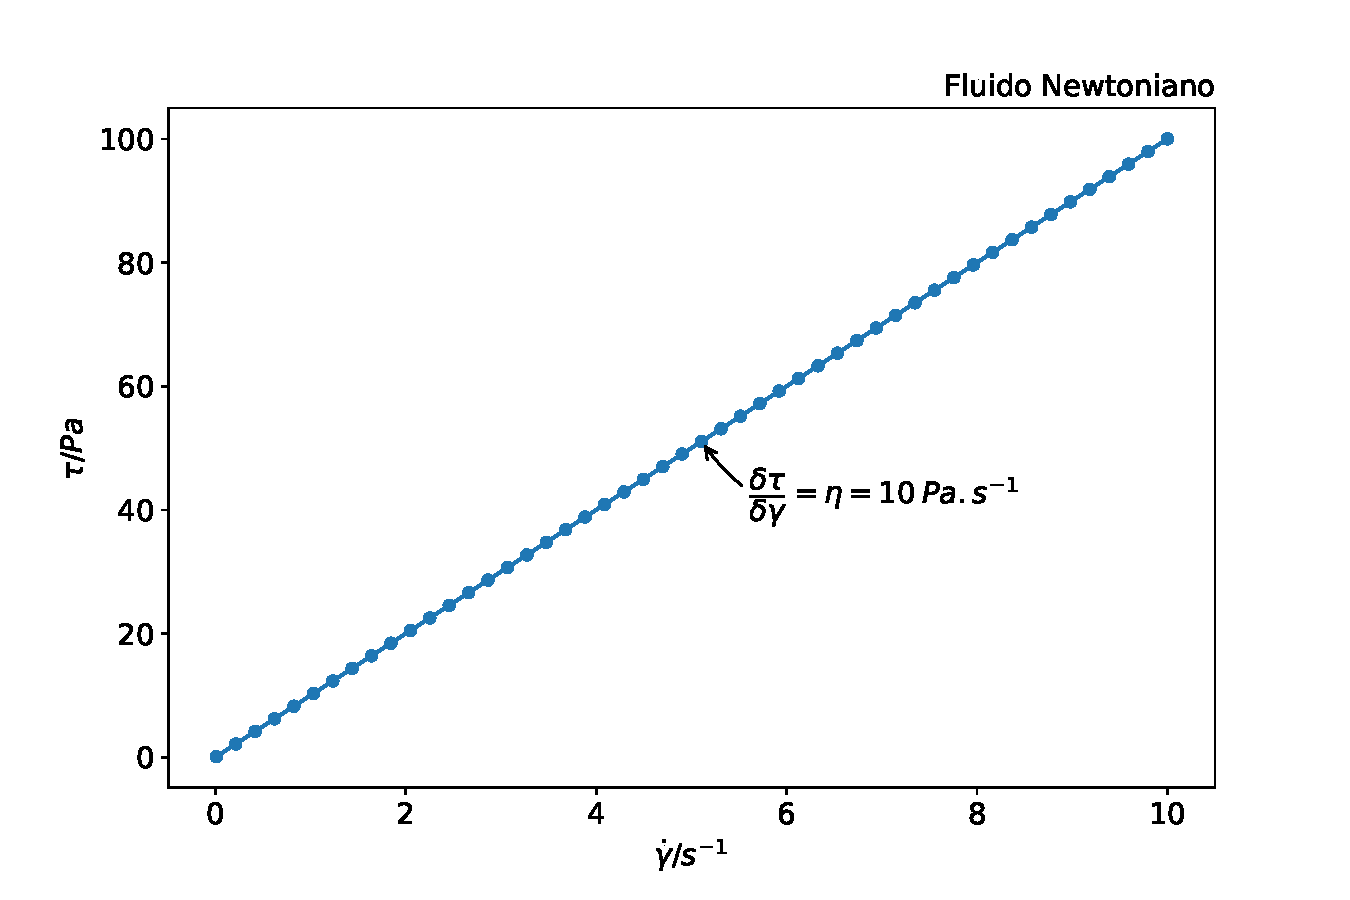
\includegraphics[width=\textwidth]{./imagens/reologia/newtoniano_exemplo_tauGP}
					\caption{\(\tau \times \dot{\gamma}\)}
					\label{fig:reol_newt_tauGP}
				\end{subfigure}%
				\begin{subfigure}[t]{.5\textwidth}
					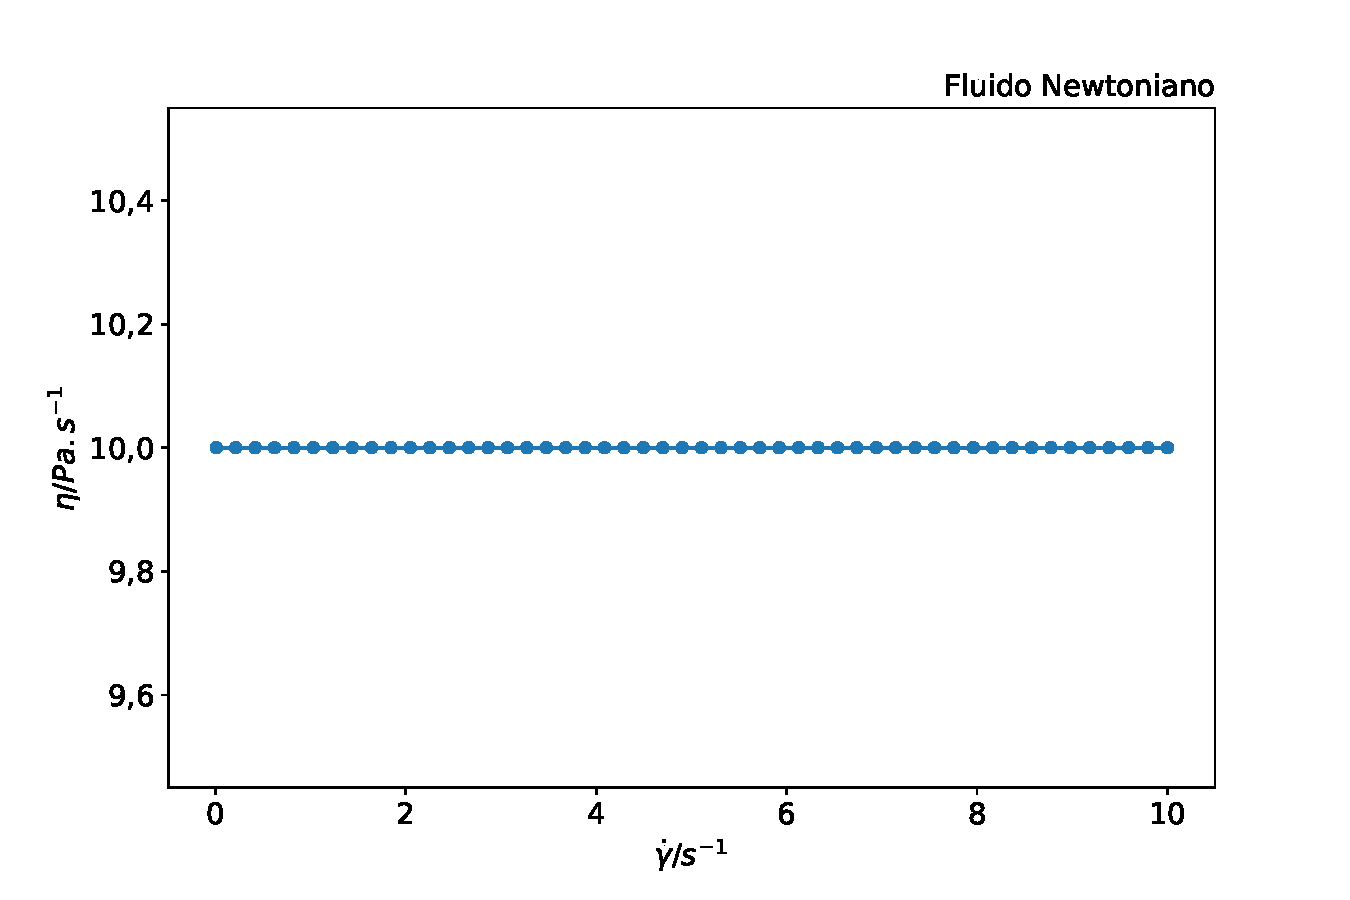
\includegraphics[width=\textwidth]{./imagens/reologia/newtoniano_exemplo_etaGP}
					\caption{\(\eta \times \dot{\gamma}\)}
					\label{fig:reol_newt_etaGP}
				\end{subfigure}
				\caption{Exemplos de curvas de fluxo. (\ref{fig:reol_newt_tauGP}) Método para obtenção da viscosidade. (\ref{fig:reol_newt_etaGP}) Dependência da viscosidade com a taxa de cisalhamento, mostrando que o valor é constante.}
				\label{fig:reol_newt_exemplos}
			\end{figure}
				
			\subsection{Sólidos Hookeanos}
			
			Sólidos hookeanos possuem uma constante elástica \(G\) que relaciona a tensão \(\tau\) aplicada e a deformação \(\gamma\) (Eq. \ref{eqn:Hooke}).
			
			\begin{equation}
				\tau = G\gamma
				\label{eqn:Hooke}
			\end{equation}
			
			A deformação de um sólido Hookeano pode ser tanto compressiva quando extensiva, dependendo do sinal de \(\gamma\), e consequentemente a tensão retornada possui a direção oposta da tensão aplicada inicialmente. 
			
			O modelo físico associado ao sólido Hookeano é a mola. É possível que uma mola, quando estendida demasiadamente, não retorne à sua extensão original. Isso ocorre porque a Eq. \ref{eqn:Hooke} se aplica somente a uma região dos possíveis valores de \(\gamma\). A fig X mostra o comportamento Hookeano de amostras.
			
			% todo: colocar uma figura do Goodwin e Hughes de viscosidade, para mostrar o comportamento não Hookeano.
			
			\subsection{Fluidos não-Newtonianos}
			
			Fluidos que não obedecem a lei de Newton (Eq. \ref{eqn:Newton}), portanto possuem valores de viscosidade dependentes da taxa de cisalhamento, são chamados de fluidos não-Newtonianos. Dentro dessa classificação, há vários tipos de fluido, dependendo de como \(\eta\) varia com (\(\dot{\gamma}\)). Alguns dos tipos possíveis são:
			
			\begin{itemize}[noitemsep]
				\item Plásticos: Viscosidade inicial é muito alta ou, teoricamente, infinita, até a tensão atingir um valor específico, chamado de tensão limite ou \emph{yield-stress}, quando o material começa a fluir. Exemplo: Manteiga, géis. % todo: achar se o termo é tensão limite mesmo
				\item Pseudoplásticos ou \emph{shear-thinning}: Viscosidade alta, mas finita, em baixas taxas de cisalhamento, e decai com o aumento da taxa de cisalhamento, atingindo um valor mínimo. Exemplo: soluções de micelas gigantes.
				\item Dilatantes: Viscosidade baixa a baixas taxas de cisalhamento, e aumenta com o aumento da taxa. Exemplo: Dispersões de amido em água.
			\end{itemize}
			
			% Todo: colocar a figura dos vários tipos de comportamento aqui.
			
			% todo: pensar melhor sobre isso de contribuições elásticas e viscosas. O que eu escrevi aqui é o oposto do que aparece no diagrama de frequência, com a viscosidade complexa. Qual é a relação?
			
			Sob taxas de cisalhamento baixas, micelas gigantes em solução estão emaranhadas. Isso dificulta a movimentação do solvente e da solução como um todo, resultado em uma viscosidade aparente alta. Nesse regime, o comportamento elástico predomina. Quanto maior for o entrelaçamento das micelas, maior é a contribuição do comportamento elástico, e maior é a viscosidade aparente. À medida que a taxa é aumentada, as micelas gigantes começam a se alinhar ao fluxo, de modo a diminuir o gradiente de velocidade que cada cadeia sente. Isso facilita o fluxo e diminui a estruturação que resulta no comportamento elástico, o que acaba diminuindo a viscosidade aparente.
			
			Após um valor específico de taxa de cisalhamento, a viscosidade atinja um mínimo pois não há mais como aumentar o alinhamento das micelas. Nessa situação, a viscosidade aparente é predominantemente devido ao solvente, e a contribuição Newtoniana é predominante. A figura \ref{fig:reol_pseudoplastico_exemplos} mostra a curva de fluxo de um material pseudoplástico, tanto .\footnote{Construção: vide apêndice \ref{sec:apn_tratamento_CF}. Parâmetros: Modelo de Carreau, \(\eta_0=10\), \(\eta_{\infty}=1\), \(\dot{\gamma}_b=10\), \(n=10\).} É possível que as cadeias comecem a se estruturar, formando \emph{shear induced structures}, mas isso não foi observado neste trabalho.
	
			\begin{figure}[H]
				\begin{subfigure}[t]{.5\textwidth}
					\includegraphics[width=\textwidth]{./imagens/reologia/pseudoplastico_tau}
					\caption{\(\tau \times \dot{\gamma}\)}
					\label{fig:reol_pseudo_tauGP}
				\end{subfigure}%
				\begin{subfigure}[t]{.5\textwidth}
					\includegraphics[width=\textwidth]{./imagens/reologia/pseudoplastico_eta}
					\caption{\(\eta \times \dot{\gamma}\)}
					\label{fig:reol_pseudo_etaGP}
				\end{subfigure}
				\caption{Exemplos de curvas de fluxo de um fluido pseudoplástico. (\ref{fig:reol_newt_tauGP}) Tensão aplicada em função da taxa de cisalhamento. (\ref{fig:reol_newt_etaGP}) Derivada de (\ref{fig:reol_newt_tauGP}) em função da taxa de cisalhamento.}
				\label{fig:reol_pseudoplastico_exemplos}
			\end{figure}
			
			No entanto, as curvas de fluxo são frequentemente plotadas na escala log-log. Nesse tipo de gráfico (Fig. \ref{fig:reol_pseudoplastico_loglog}), é possível observar a região com viscosidade constante em baixas taxas de cisalhamento, chamada de platô Newtoniano, devido à sua constância. Essa valor também é chamado de viscosidade no repouso, \(\eta_0\).
			
			\begin{figure}[H]
				\centering
				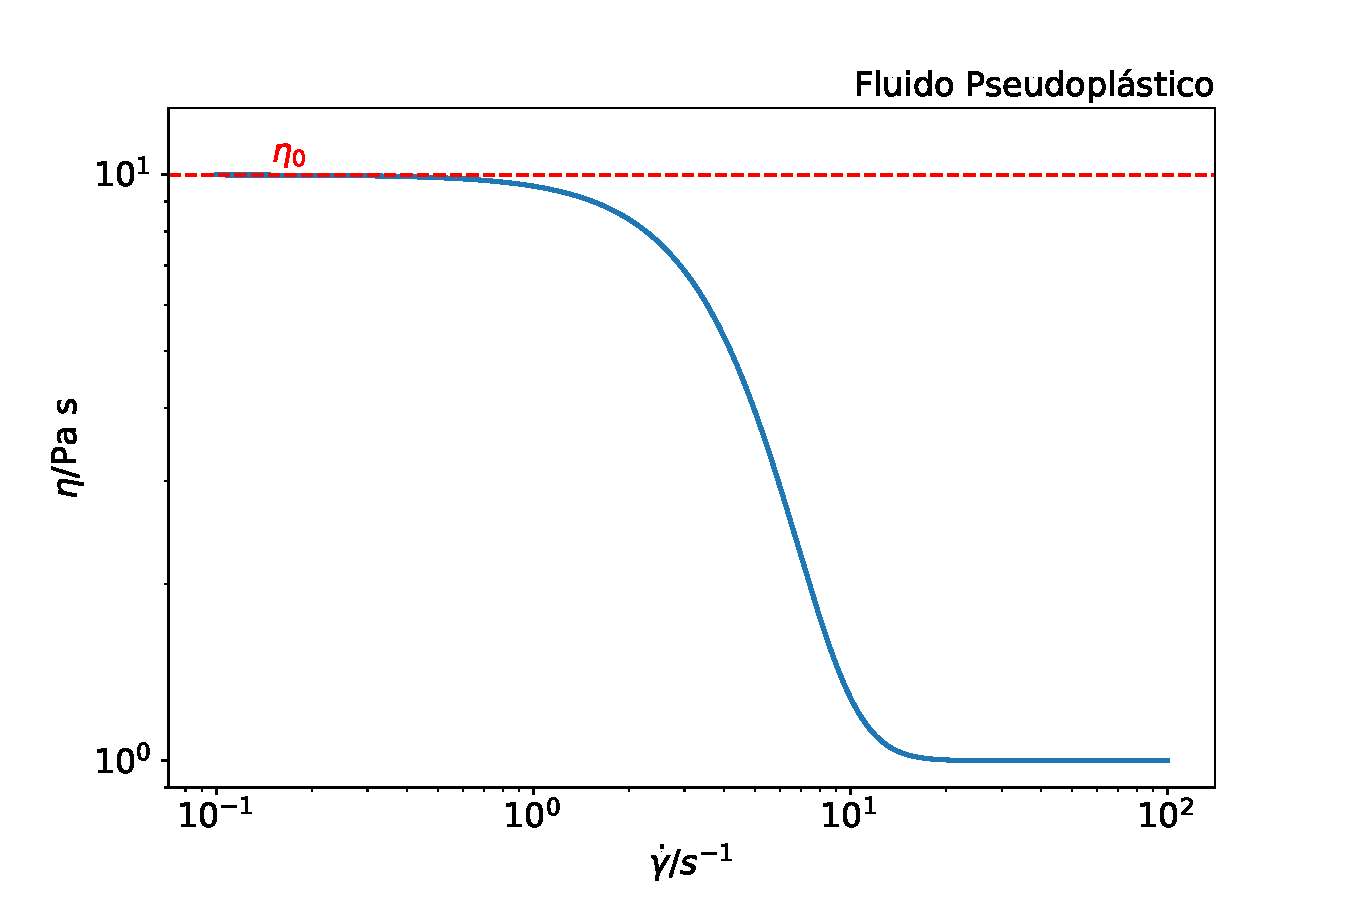
\includegraphics[width=0.7\textwidth]{./imagens/reologia/Pseudoplastico_loglog}
				\caption{Curva de fluxo de um fluído pseudoplástico na escala log-log, mostrando o valor da viscosidade no repouso, \(\eta_0\).}
				\label{fig:reol_pseudoplastico_loglog}
			\end{figure}
		
			Para obter o valor da viscosidade no repouso, é possível tanto realizar um ajuste linear da região inicial na escala log-log, ou ajustar um modelo à curva, como o modelo de Cross, Carreau e Carreau-Yasuda. Mais informações sobre a modelagem estão no apêndice \ref{sec:apn_tratamento_CF}.

		\section{Reologia oscilatória}
			\subsection{Princípios e aquisição de dados}
			
			As análises oscilatórias podem ser utilizadas para obter informações reológicas mais completas sobre um material. Variando-se a frequência de perturbação, é possível obter o espectro mecânico do material, onde se observa as contribuições elástica e viscosa em função da frequência de perturbação mecânica.
			
			Ao material, é aplicada uma deformação \(\gamma\) que varia com o tempo de acordo com a Eq. \ref{eqn:osc_gamma_t}.
			
			\begin{equation}
				\gamma(t)=\gamma_0\cos(\omega t)
				\label{eqn:osc_gamma_t}
			\end{equation}
			
			\noindent onde \(\gamma_0\) é a deformação máxima e \(\omega\) é a frequência de perturbação. As deformações aplicadas ao material devem ser tais que não ocorra desestruturação do mesmo. Por exemplo, uma deformação muito grande pode causar a quebra de ligações químicas de um polímero, o que altera irreversivelmente as suas características reológicas. Por esse motivo, é necessário modular também a tensão aplicada.
			
			Um material elástico responde à deformação imediatamente com uma força no sentido oposto ao sentido da deformação. Já materiais viscosos respondem à deformação quando há uma mudança na direção, ou seja, a resposta desses materiais é totalmente defasada em relação à aplicação da deformação. Já materiais viscoelásticos, por terem componentes de ambos os tipos, possuem uma defasagem intermediária. O grau dessa defasagem é proporcional ao grau de comportamento elástico e viscoso. Levando isso em consideração, a tensão \(\tau\)  é expressa de acordo com a Eq. \ref{eqn:osc_tau_t}.
			
			\begin{equation}
				\tau = \tau_0\cos(\omega t - \theta)
				\label{eqn:osc_tau_t}
			\end{equation}
			
			\noindent onde \(\tau_0\) é a tensão máxima (determinada no experimento oscilatório de amplitude) e \(\theta\) é o ângulo de defasagem.
			
			As expressões \ref{eqn:osc_gamma_t} e \ref{eqn:osc_tau_t} podem ser reescritas utilizando a relação de Euler, Eq. \ref{eqn:Euler}, resultando nas expressões \ref{eqn:osc_gamma_im} e \ref{eqn:osc_tau_im}, onde utilizou-se um acento circunflexo para diferenciar as expressões. Essa transformação facilita a manipulação matemática.
			
			\begin{equation}
				e^{ix} = \cos(x) + i\sin(x)
				\label{eqn:Euler}
			\end{equation}
			
			\begin{equation}
				\hat{\gamma} = \gamma_0 e^{i\omega t}
				\label{eqn:osc_gamma_im}
			\end{equation}
			
			\begin{equation}
				\hat{\tau} = \tau_0 e^{i(\omega t - \theta)}
				\label{eqn:osc_tau_im}
			\end{equation}
			
			A partir dessas relações, é possível utilizar a equação de Hooke (Eq. \ref{eqn:Hooke}) para encontrar o módulo elástico do material, na notação imaginária, \(\hat{G}\) (Eq. \ref{eqn:osc_transform_G}).
			
			\begin{equation}
				\hat{\tau} = \hat{G}\hat{\gamma} \to \hat{G} = \dfrac{\hat{\tau}}{\hat{\gamma}}    \to 
				\hat{G} = \dfrac{\tau_0}{\gamma_0} \dfrac{e^{i(\omega t - \theta)}}{e^{i\omega t}} \to
				\hat{G} = \dfrac{\tau_0}{\gamma_0} e^{-i\theta}
				\label{eqn:osc_transform_G}
			\end{equation}
			
			Utilizando-se a equação de Euler novamente, mas voltando para o domínio dos senos e cossenos, obtemos a Eq. \ref{eqn:osc_volta_senos_G}:
			
			\begin{equation}
				\hat{G} = \dfrac{\tau_0}{\gamma_0} \left( \cos(\theta) + i\sin(\theta) \right)
				\label{eqn:osc_volta_senos_G}
			\end{equation}
			
			Nessa equação, o módulo total \(\hat{G}\) foi dividido em dois termos, um em fase à deformação \(\cos(\theta)\) e outro 90° fora de fase, \(\sin(\theta)\). Esses dois termos são diretamente relacionáveis às componentes elástica e viscosa de um material. Dessa maneira, é possível separar o módulo total complexo \(\hat{G}\) em dois módulos (Eq. \ref{eqn:osc_G_complexo}), o módulo elástico, G' (Eq. \ref{eqn:osc_g1linha}), e o módulo viscoso, G'' (Eq. \ref{eqn:osc_g2linha}).
			
			\begin{equation}
				\hat{G} = G' + iG''
				\label{eqn:osc_G_complexo}
			\end{equation}
			
			\begin{equation}
				G' = \dfrac{\tau_0}{\gamma_0} \cos(\theta)
				\label{eqn:osc_g1linha}
			\end{equation}
			
			\begin{equation}
				G'' = \dfrac{\tau_0}{\gamma_0} \sin(\theta)
				\label{eqn:osc_g2linha}
			\end{equation}
			
			Portanto, para conseguir separar os valores dos módulos G' e G'', o reômetro necessita medir o módulo total e o ângulo de defasagem, sendo possível assim separar os componentes. Vale notar que a tangente do ângulo de defasagem é a relação \(G''/G'\) (Eq. \ref{eqn:osc_tan_teta})
			
			\begin{equation}
				\tan(\theta) = \dfrac{\sin(\theta)}{\cos(\theta)} = \dfrac{G''}{G'}
				\label{eqn:osc_tan_teta}
			\end{equation}
			
			A Figura \ref{fig:osc_simulacoes} mostra uma série de simulações do modelo apresentado aqui. A deformação em função do tempo foi calculada, e o ângulo de defasagem foi aumentado gradativamente de 0° para 90°. 
			% todo: descobrir e colocar os ângulos aqui
			
			\begin{figure}[H]
				\begin{subfigure}[t]{0.3\textwidth}
					\centering
					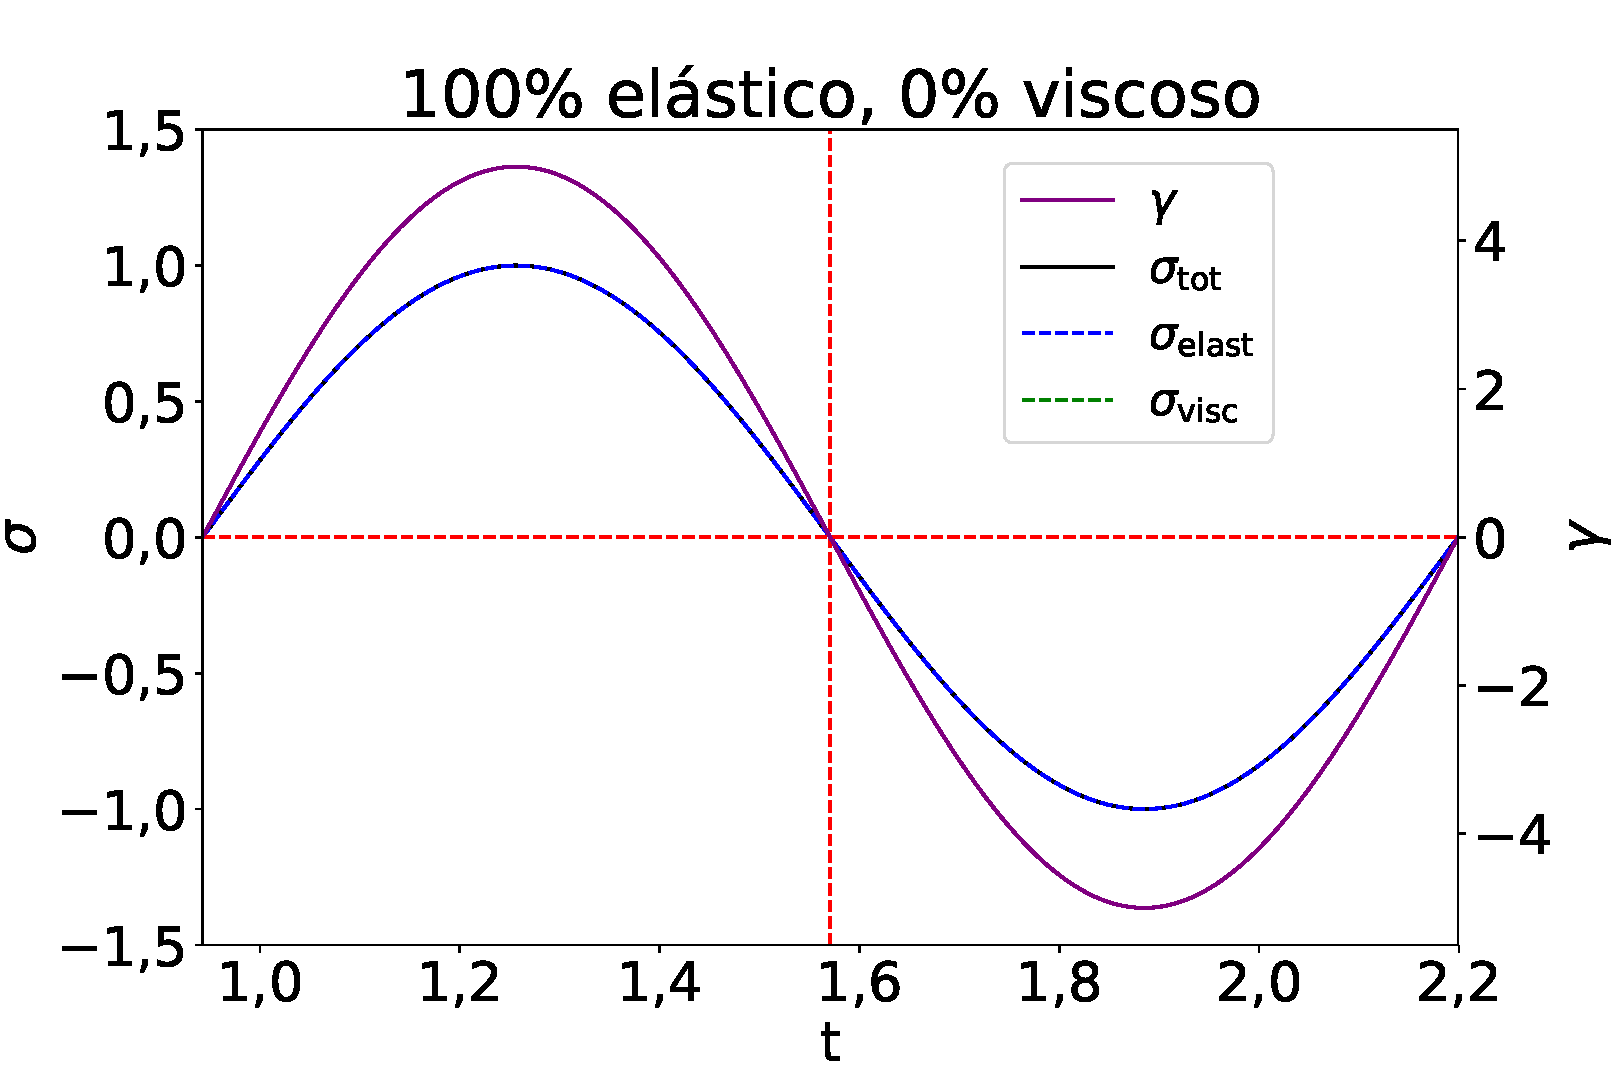
\includegraphics[width=\textwidth]{./imagens/reologia/Simulacao_visc_0}
					\caption{\(\theta=0°\)}
					\label{fig:osc_sim0}
				\end{subfigure}%
				\begin{subfigure}[t]{0.3\textwidth}
					\centering
					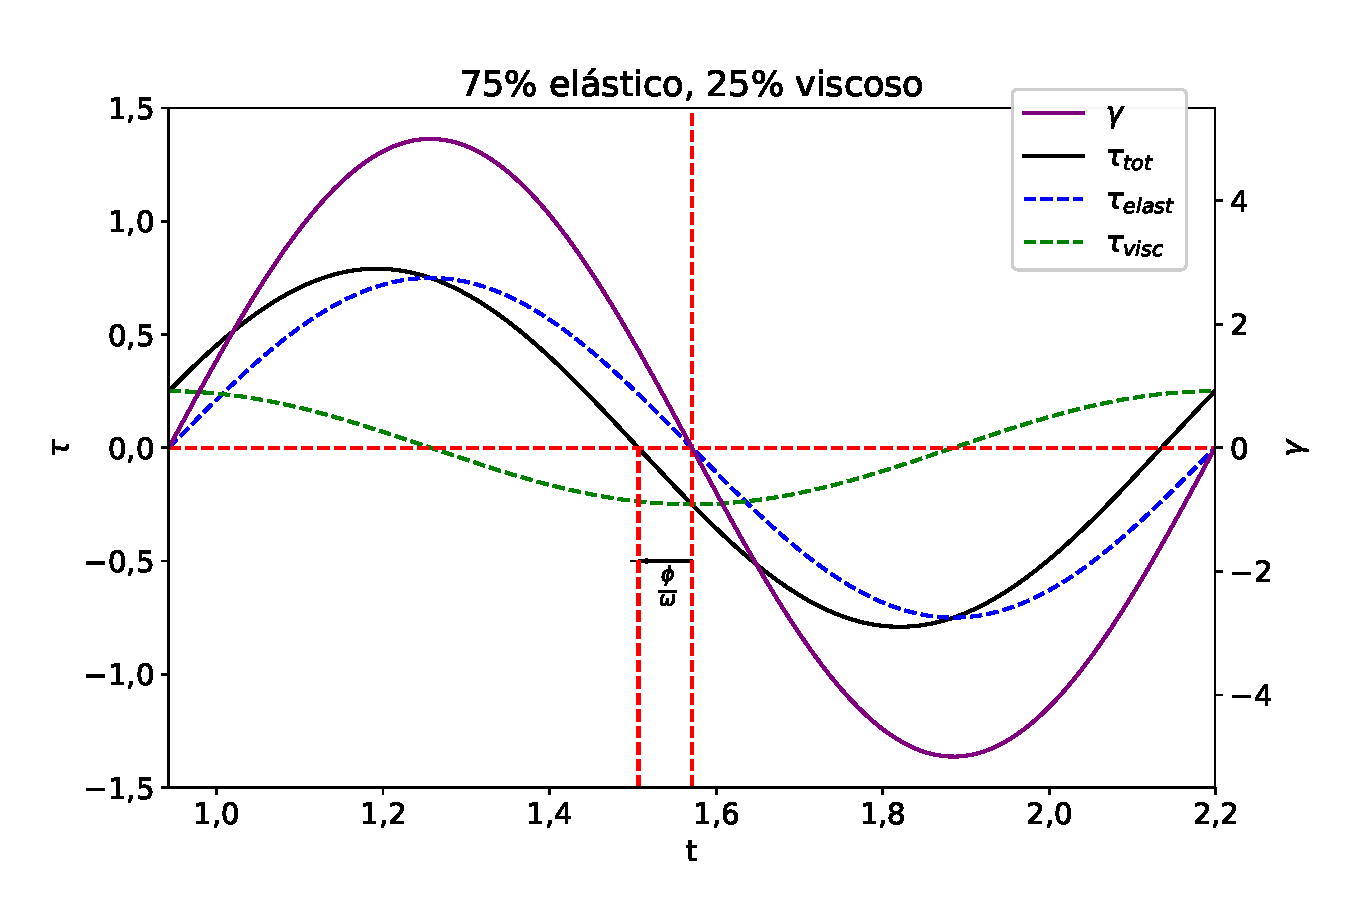
\includegraphics[width=\textwidth]{./imagens/reologia/Simulacao_visc_25}
					\caption{\(\theta=18°\)}
					\label{fig:osc_sim25}
				\end{subfigure}%
				\begin{subfigure}[t]{0.3\textwidth}
					\centering
					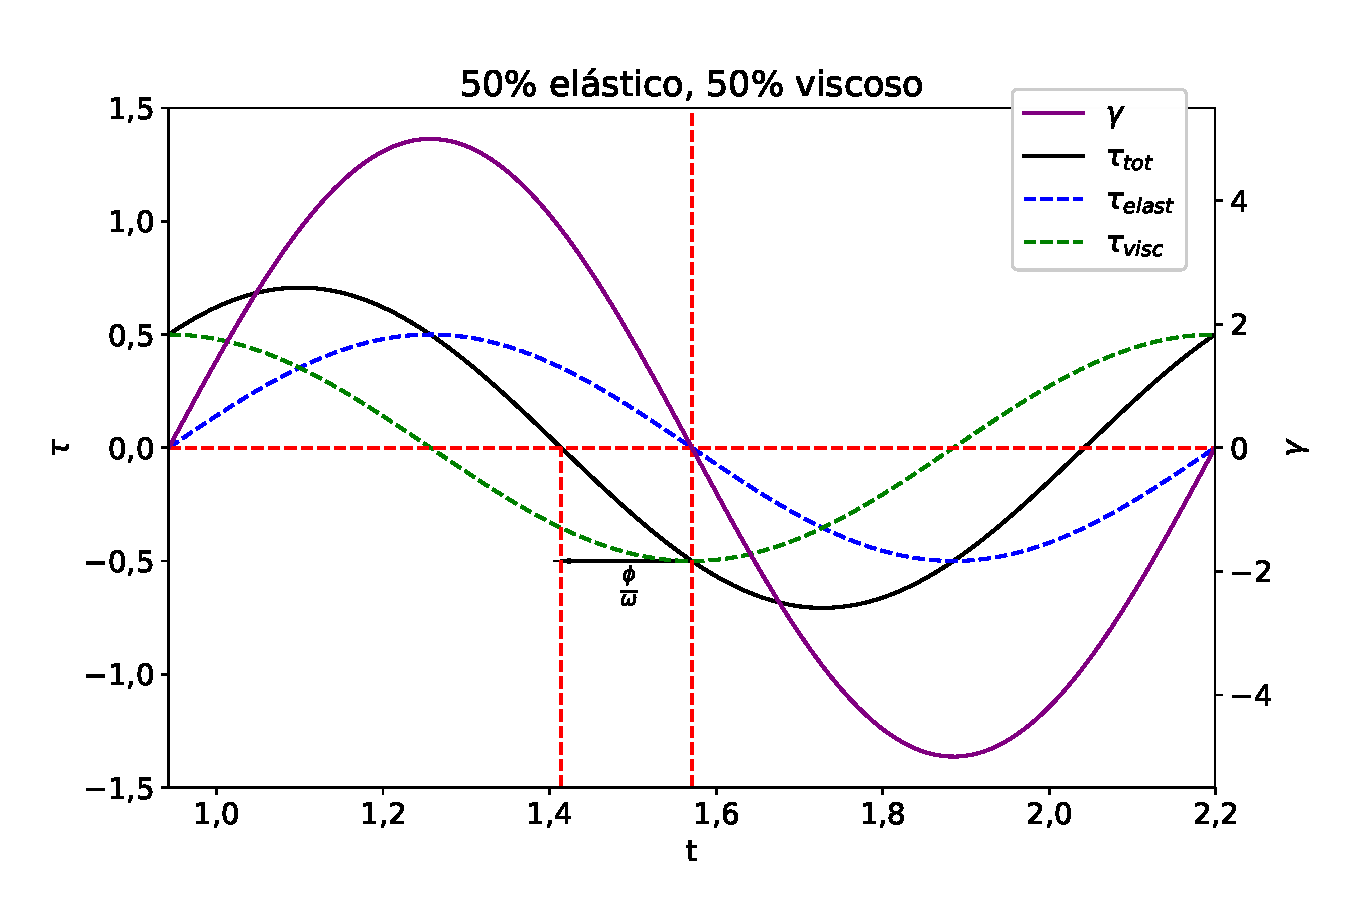
\includegraphics[width=\textwidth]{./imagens/reologia/Simulacao_visc_50}
					\caption{\(\theta=45°\)}
					\label{fig:osc_sim50}
				\end{subfigure}
			
				\begin{subfigure}[t]{0.3\textwidth}
					\centering
					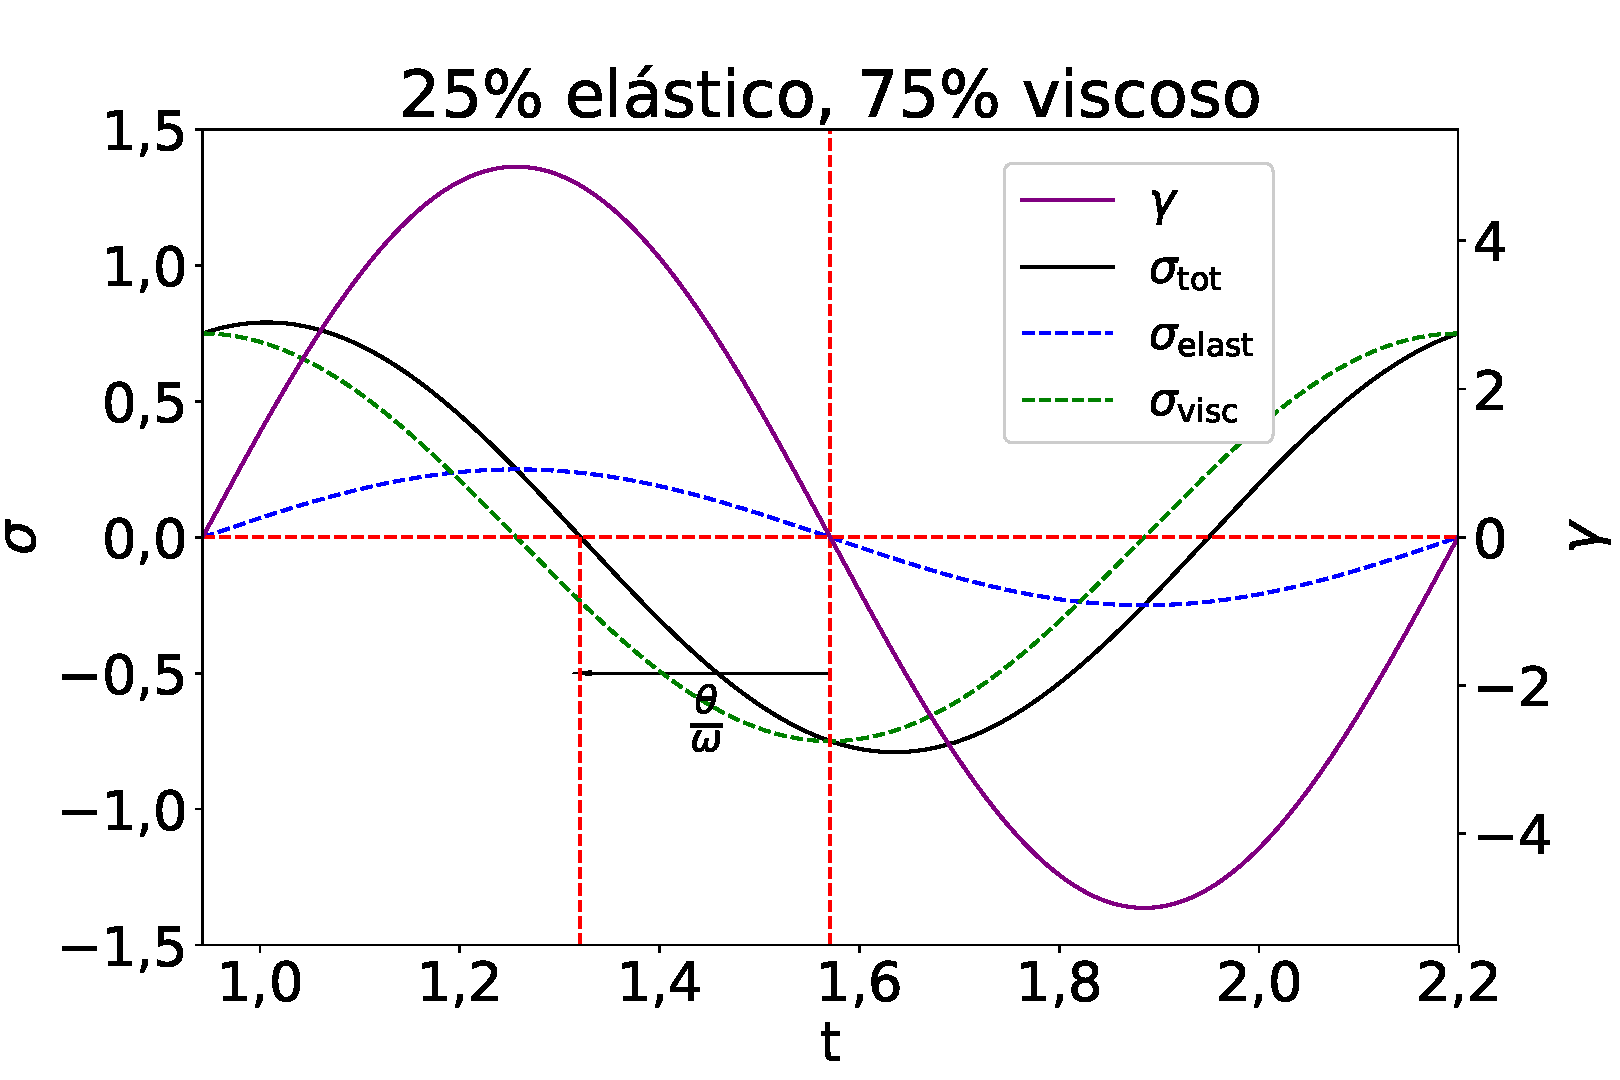
\includegraphics[width=\textwidth]{./imagens/reologia/Simulacao_visc_75}
					\caption{\(\theta=72°\)}
					\label{fig:osc_sim75}
				\end{subfigure}%
				\begin{subfigure}[t]{0.3\textwidth}
					\centering
					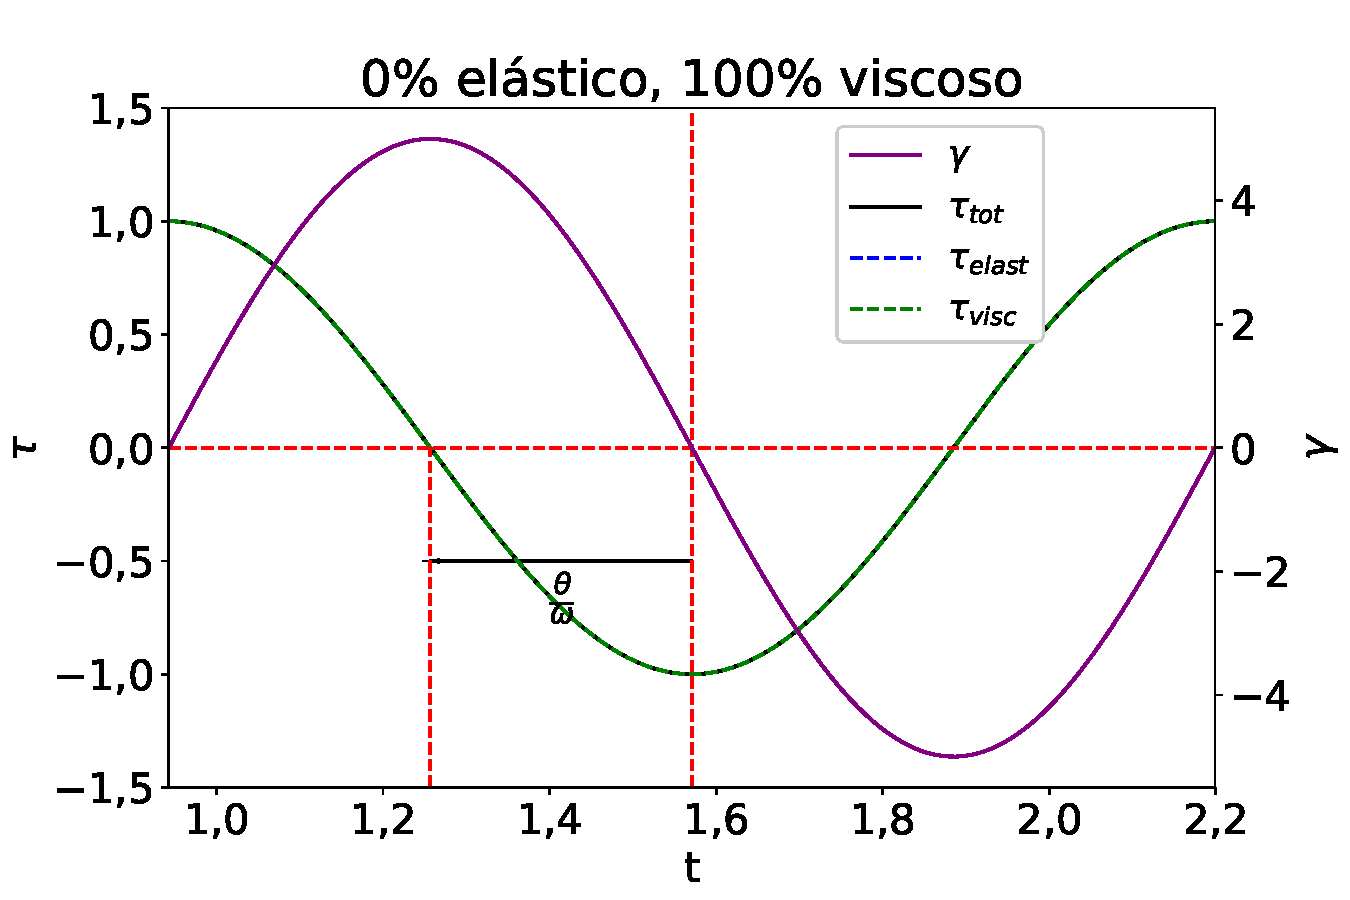
\includegraphics[width=\textwidth]{./imagens/reologia/Simulacao_visc_100}
					\caption{\(\theta=90°\)}
					\label{fig:osc_sim100}
				\end{subfigure}%
%				\begin{subfigure}[t]{0.3\textwidth}
%					\centering
%					\includegraphics[width=\textwidth]{}
%					\label{fig:}
%				\end{subfigure}
			\caption{Simulações do comportamento de um fluido sob cisalhamento cossenoidal. As imagens mostram a deformação \(\gamma\) em função do tempo, a tensão total \(\tau\) de resposta em função do tempo, decomposta em suas componentes elástica e viscosa. No título de cada gráfico está a contribuição, em porcentagem, de cada componente do material. O ângulo de defasagem está ilustrado na figura.}
			\label{fig:osc_simulacoes}
			\end{figure}  % todo: colocar o código para essa figura nos apêndices
			
			\subsection{Modelo de Maxwell}
			
			O modelo de Maxwell é construído juntando-se um elemento elástico (mola) e um elemento viscoso (dissipador), ideais, em série. A Figura \ref{fig:ilust_modelo_maxwell} ilustra essa construção.
			
			\begin{figure}[H]
				\centering
				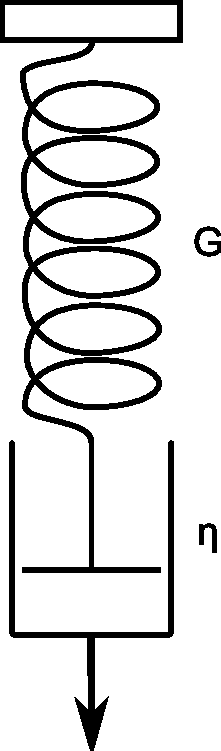
\includegraphics[width=1.5cm]{./imagens/reologia/maxwell_mola_dissipador}
				\caption{Modelo de Maxwell: Mola com constante elástica \(G\) e dissipador com constante viscosa \(\eta\) em série}
				\label{fig:ilust_modelo_maxwell}
			\end{figure}

			 É possível expressar a taxa de cisalhamento do modelo de Maxwell como a soma das taxas de cisalhamento dos elementos individuais (Eq. \ref{eqn:Maxwell_soma}). 
			 
			\begin{equation}
				\dot{\gamma}_{\textrm{total}} =  \dot{\gamma}_{\textrm{viscoso}} + \dot{\gamma}_{\textrm{elástico}} \to
				\dfrac{d\gamma}{dt} = \dfrac{1}{\eta}\tau + \dfrac{1}{G}\dfrac{d\tau}{dt}
				\label{eqn:Maxwell_soma}
			\end{equation}
			
			Para uma deformação constante, \(\frac{d\gamma}{dt}=0\), a Eq. \ref{eqn:Maxwell_soma} se torna uma equação diferencial (Eq. \ref{eqn:Maxwell_diferencial}).
			
			\begin{equation}
				\dfrac{1}{\eta}\tau + \dfrac{1}{G}\dfrac{d\tau}{dt} = 0
				\label{eqn:Maxwell_diferencial}
			\end{equation}
			
			Utilizando as condições de contorno necessárias, essa equação pode ser resolvida, resultando em (Eq. \ref{eqn:Maxwell_dif_resolvida}):
			
			\begin{equation}
				\tau(t) = \tau_0 e^{\left( -\frac{G}{\eta}t \right)}
				\label{eqn:Maxwell_dif_resolvida}
			\end{equation}
			
			O termo exponencial na Eq. \ref{eqn:Maxwell_dif_resolvida} possui unidade de tempo e é a relação entre as componentes elástica e viscosa do material. Essa relação recebe o nome de tempo de relaxação, \(\tau_{\textrm{rel}}\) (Eq. \ref{eqn:Maxwell_tempo_rel_def})
			
			\begin{equation}
				\tau(t) = \tau_0 e^{\sfrac{-t}{\tau_{\textrm{rel}}}}
				\label{eqn:Maxwell_tempo_rel_def}
			\end{equation}
		
			O tempo de relaxação é o tempo em que a tensão inicial demora para cair ao valor de \(\sfrac{1}{e}\) do valor inicial. É interessante notar que em tempos pequenos, relativos a \(\tau_{\textrm{rel}}\), o material responde com a tensão inicial total. Essa é a resposta imediata da mola. Porém, com o tempo, à medida que \(t\to\tau_{\textrm{rel}}\), a tensão começa a decair exponencialmente e depois, em \(t \gg \tau_{\textrm{rel}}\), tende a zero. Nessa situação, o dissipador difundiu toda a energia inicial aplicada.
			
			A expressão \ref{eqn:Maxwell_soma} pode ser rearranjada utilizando o tempo de relaxação (\ref{eqn:Maxwell_tempo_rel_def}).
			
			\begin{equation}
				\dfrac{d\gamma}{dt} = \dfrac{1}{\eta}\tau + \dfrac{1}{G}\dfrac{d\tau}{dt} \to 
				\tau = -\dfrac{\eta}{G} \dfrac{d\tau}{dt} + \eta\dfrac{d\gamma}{dt} =
				-\tau_{\textrm{rel}} \dfrac{d\tau}{dt} + \eta\dfrac{d\gamma}{dt}
				\label{eqn:Maxwell_inicio_g1g2}
			\end{equation}
			
			É possível substituir as expressões de tensão e \ref{eqn:osc_gamma_im} e \ref{eqn:osc_tau_im} na expressão \ref{eqn:Maxwell_inicio_g1g2} para obter uma expressão em função do tempo, da frequência e do ângulo de fase. Já realizando as derivações, obtemos:
			
			\begin{equation}
				\tau_0 e^{i \left( \omega t - \theta \right)} = - \tau_{\textrm{rel}} \tau_0 i\omega e^{i \left( \omega t - \theta \right)}     +       \eta i\omega\gamma_0e^{i\omega t}
				\label{eqn:Maxwell_substituicao}
			\end{equation}
			
			Em comum a todos os termos é a constante \(e^{i\omega t}\). Dividindo ambos os lados por essa constante, agrupando os termos com \(e^{-i\theta}\) e substituindo a viscosidade por \(G\tau_{\textrm{rel}}\), temos:
			
			\begin{equation}
				\tau_0e^{-i\theta} \left(   1 + i\omega\tau_{\textrm{rel}}  \right) = i\omega G\tau_{\textrm{rel}}\gamma_0 \to
				\tau_0e^{-i\theta} = \dfrac{i\omega G\tau_{\textrm{rel}}\gamma_0}{\left(   1 + i\omega\tau_{\textrm{rel}}  \right)}
				\label{eqn:Maxwell_intermediario}
			\end{equation}
			
			O termo à esquerda da Eq. \ref{eqn:Maxwell_intermediario} é similar à definição do módulo elástico complexo, Eq. \ref{eqn:osc_transform_G}, sendo necessário somente dividir ambos os lados por \(\gamma_0\). Realizando a substituição, temos:
			
			\begin{equation}
				\hat{G} = \dfrac{\tau_0e^{-i\theta}}{\gamma_0} = \dfrac{i\omega G\tau_{\textrm{rel}}}{\left(   1 + i\omega\tau_{\textrm{rel}}  \right)}
				\label{eqn:Maxwell_complexo_antes_sep}
			\end{equation}
			
			Seguindo o princípio de que o módulo complexo \(\hat{G}\) pode ser dividido em uma parte imaginária e uma parte real, podemos realizar o mesmo com a Eq. \ref{eqn:Maxwell_complexo_antes_sep} multiplicando-se a fração por \(\frac{\left(   1 - i\omega\tau_{\textrm{rel}}  \right)}{\left(   1 - i\omega\tau_{\textrm{rel}}  \right)}\).
			
			\begin{equation}
				\hat{G} = \dfrac{  i\omega G\tau_{\textrm{rel}} - i^2 \omega^2 G \tau_{\textrm{rel}}^2        }{  1 - i^2\omega^2 \tau_{\textrm{rel}}^2          }
				\label{eqn:Maxwell_complexo_antes_sep2}
			\end{equation}
			
			Separando as partes imaginárias das partes reais e substituindo \(i^2 = -1\):
			
			\begin{equation}
				\hat{G} = \dfrac{   \omega^2 G \tau_{\textrm{rel}}^2       }{  1 + \omega^2 \tau_{\textrm{rel}}^2      } + i \dfrac{   \omega G \tau_{\textrm{rel}}        }{ 1 + \omega^2 \tau_{\textrm{rel}}^2 }
				\label{eqn:Maxwell_substituido}
			\end{equation}
			
			Seguindo a expressão \ref{eqn:osc_G_complexo}, \(\hat{G} = G' + iG''\), podemos definir o módulo elástico de acordo com o modelo de Maxwell como:
			
			\begin{equation}
				G' = \dfrac{ G \omega^2 \tau_{\textrm{rel}}^2   }{  1 + \omega^2 \tau_{\textrm{rel}}^2      }
				\label{eqn:Maxwell_G1_def}
			\end{equation}
			
			E o módulo viscoso, G'', como:
			
			\begin{equation}
				G'' = \dfrac{  G \omega  \tau_{\textrm{rel}}        }{ 1 + \omega^2 \tau_{\textrm{rel}}^2 }
				\label{eqn:Maxwell_G2_def}
			\end{equation}
			
			É interessante notar que a relação \(\sfrac{G''}{G'}\), que equivale a \(\tan(\theta)\) (\ref{eqn:osc_tan_teta}), também se relaciona com o tempo de relaxação:
			
			\begin{equation}
				\tan(\theta) = \dfrac{G''}{G'} = \dfrac{1}{\omega\tau_{\textrm{rel}}}
				\label{eqn:Maxwell_cruzamento}
			\end{equation}
			
			Com isso, é possível determinar o tempo de relaxação de um fluido Maxwelliano através da frequência do ponto de cruzamento de G' e G''. Lembrando que \(\omega\) é a frequência de perturbação, e o inverso da frequência é o tempo de observação, podemos relacionar essa relação com o número de Deborah, Eq. \ref{eqn:Deborah}.
			
			\begin{equation}
				\dfrac{1}{\omega\tau_{\textrm{rel}}} = \dfrac{ t_{\textrm{observação}  }}{ \tau_{\textrm{rel}}  } = \dfrac{1}{D_e}
				\label{eqn:Maxwell_cruzamento_Deborah}
			\end{equation}

			A reologia oscilatória geralmente é expressa em termos de G' e G'' em função da frequência, na escala logarítmica. A Fig. \ref{fig:modelo_maxwell} mostra duas curvas simuladas para um material com tempo de relaxação de 10 s.$rad^{-1}$ e um módulo \(G\) de 10 Pa. Nessa figura estão mostrado como se obtêm visualmente os parâmetros \(G\) e \(\tau_{\textrm{rel}}\).
			
			\begin{figure}[H]
				\centering
				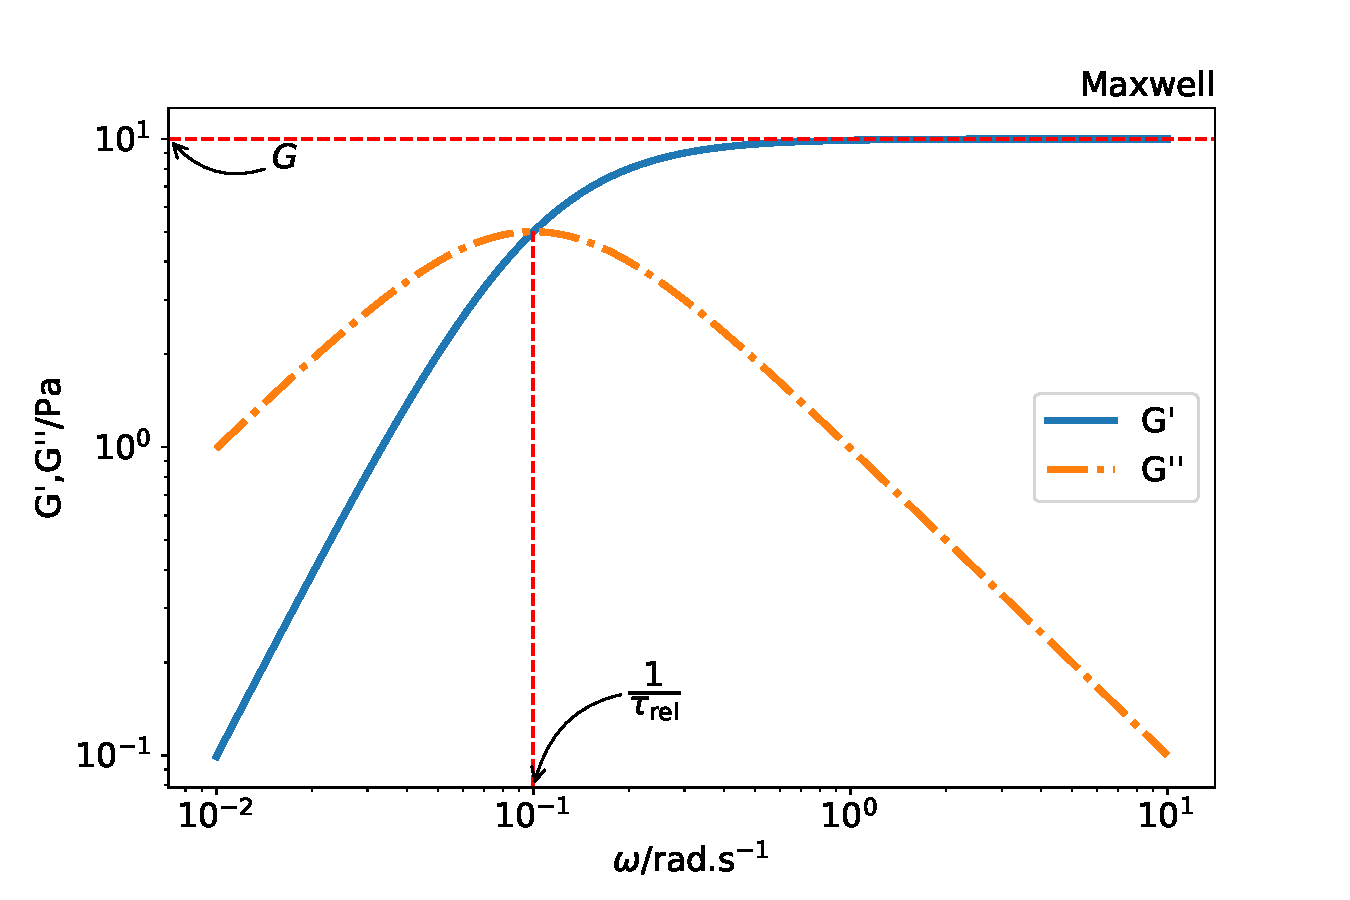
\includegraphics[width=0.7\textwidth]{./imagens/reologia/modelo_maxwell}
				\caption{Espectro mecânico de acordo com o modelo de Maxwell}
				\label{fig:modelo_maxwell}
			\end{figure}
						
			Micelas gigantes, em vários regimes, obedecem muito bem o modelo de Maxwell. É possível interpretar esse comportamento da seguinte maneira. Em baixas frequências de perturbação (longos tempos), as micelas possuem tempo suficiente para deslizar umas pelas outras, então a maior parte da energia fornecida é perdida, logo o módulo viscoso, ou de perda, possui valores altos. Em frequências altas, a rede micelar e os entrelaçamentos conseguem armazenar a energia, não possuindo tempo suficiente para deslizar, então o módulo elástico, ou de armazenamento, é alto. Na região intermediária, ambos os mecanismos estão presentes, parte da energia é perdida e parte é armazenada, sendo que no ponto de cruzamento, exatamente metade da energia é preservada e metade é perdida.
			
			Para a obtenção de valores mais confiáveis para os parâmetros, é necessário realizar um ajuste dessas curvas. Porém, existem duas curvas que são descritas pelos mesmos parâmetros. Ao invés de se fazer dois ajustes e encontrar quatro parâmetros, é ideal realizar um ajuste das duas curvas simultaneamente. Isso pode ser feito minimizando-se um vetor com os resíduos das duas curvas concatenados. Isso pode ser feito utilizando-se, por exemplo, o Excel, com a ferramenta \emph{Solver} para minimizar o resíduo.
			
			\subsection{Modelos mais complexos}
			
			Experimentalmente, existem divergências entre o modelo de Maxwell e os espectros mecânicos dos materiais. Geralmente, essas divergências aparecem devido ao aparecimento de outros  mecanismos de relaxação em frequências mais altas. Para isso, existem alguns modelos que visam corrigir o modelo de Maxwell, afetando principalmente essa região.
			
			Uma possível correção é utilizar dois elementos de Maxwell em série, produzindo um modelo que tem dois tempos de relaxação e dois módulos (Eqs. \ref{eqn:modelo_doismodos_g1}, \ref{eqn:modelo_doismodos_g2}).
			
			\begin{equation}
				G' = \dfrac{ G_1 \omega^2 \tau_{\textrm{rel,1}}^2   }{  1 + \omega^2 \tau_{\textrm{rel,1}}^2      } + \dfrac{ G_2 \omega^2 \tau_{\textrm{rel,2}}^2   }{  1 + \omega^2 \tau_{\textrm{rel,2}}^2      }
			\label{eqn:modelo_doismodos_g1}
			\end{equation}
		
			\begin{equation}
				G'' = \dfrac{  G_1 \omega  \tau_{\textrm{rel,1}}        }{ 1 + \omega^2 \tau_{\textrm{rel,1}}^2 } + \dfrac{  G_2 \omega  \tau_{\textrm{rel,2}}        }{ 1 + \omega^2 \tau_{\textrm{rel,2}}^2 }
			\label{eqn:modelo_doismodos_g2}
			\end{equation}
			
			% todo: a viscosidade do Oldroyd é para isso mesmo?
			
			O modelo de Oldroyd é praticamente idêntico ao modelo de Maxwell, e introduz somente um termo relativo à viscosidade do solvente para altas frequências de G'' (Eq. \ref{eqn:modelo_oldroyd_g2}). G' é inalterado.
			
			\begin{equation}
				G'' =\dfrac{  G \omega  \tau_{\textrm{rel}}        }{ 1 + \omega^2 \tau_{\textrm{rel}}^2 } + \eta_{\infty} * \omega
				\label{eqn:modelo_oldroyd_g2}
			\end{equation}
			
			O modelo mais diferente do modelo de Maxwell é o modelo de Jeffreys, que possui as seguintes formas:
			
			\begin{equation}
				G' = \dfrac{G \omega^{2} \tau_{\textrm{rel,1}} \left(\tau_{\textrm{rel,1}} - \tau_{\textrm{rel,2}}\right)}{1 + \omega^{2} \tau_{\textrm{rel,1}}^{2}}
				\label{eqn:modelo_jeffreys_g1}
			\end{equation}
			
			\begin{equation}
				G'' = \dfrac{G \omega \tau_{\textrm{rel,1}} \left(\omega^{2} \tau_{\textrm{rel,1}} \tau_{\textrm{rel,2}} + 1\right)}{1 + \omega^{2} \tau_{\textrm{rel,1}}^{2}}
				\label{eqn:modelo_jeffreys_g2}
			\end{equation}
			
			% todo: verificar na literatura essas equações.
			
			A Figura \ref{fig:comparativo_modelos} compara os três modelos mais complexos apresentados com o modelo de Maxwell. 
			
			\begin{figure}[H]
				\begin{subfigure}[t]{.5\textwidth}
					\centering
					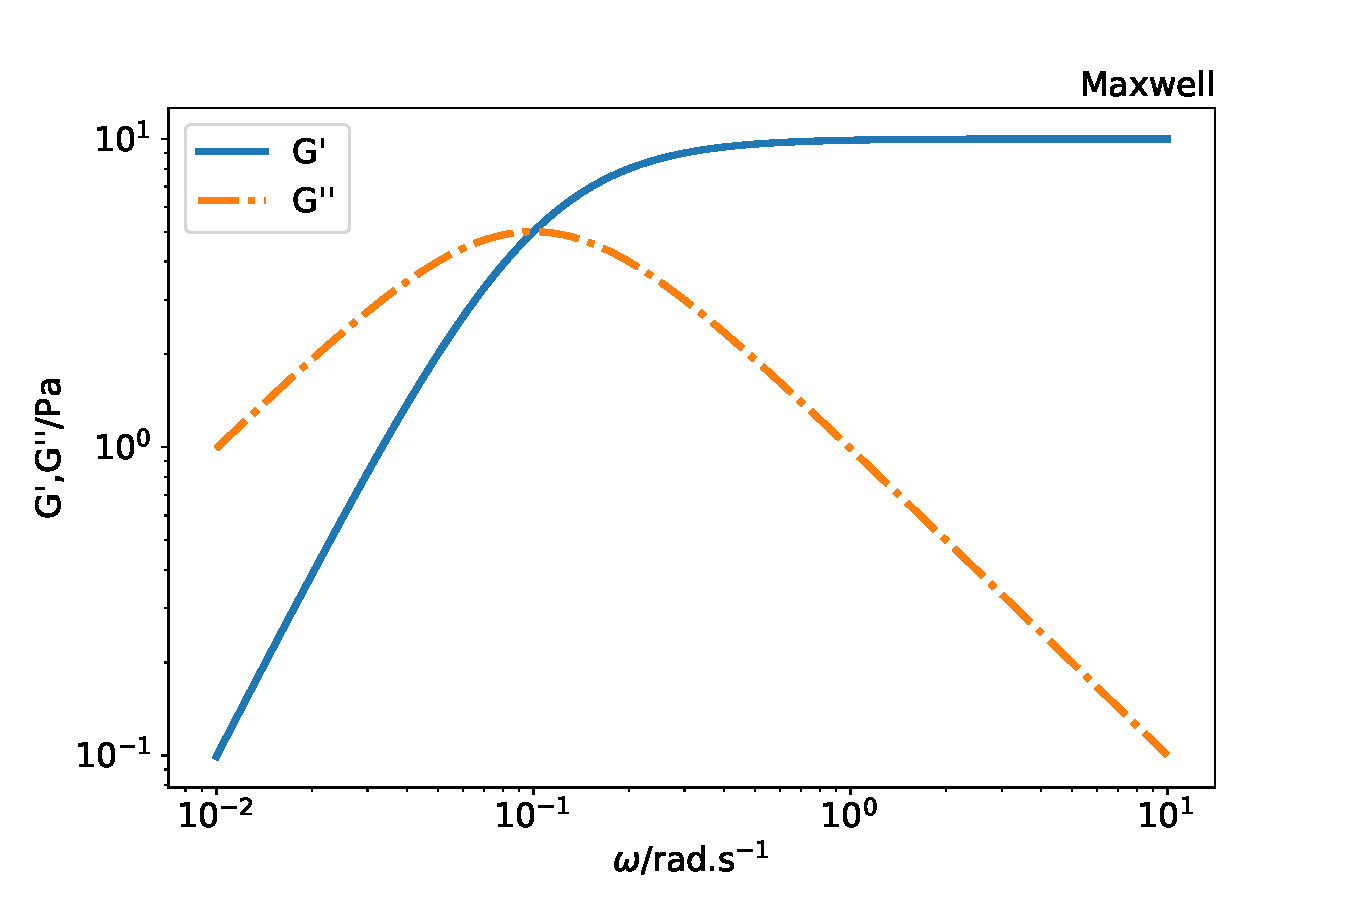
\includegraphics[width=\textwidth]{./imagens/reologia/modelos_comparativo_max}
					\caption{Maxwell. \(G=10, \tau_{\textrm{rel}}=10\)}
					\label{fig:comparativo_modelo_maxwell}
				\end{subfigure}%
				\begin{subfigure}[t]{.5\textwidth}
					\centering
					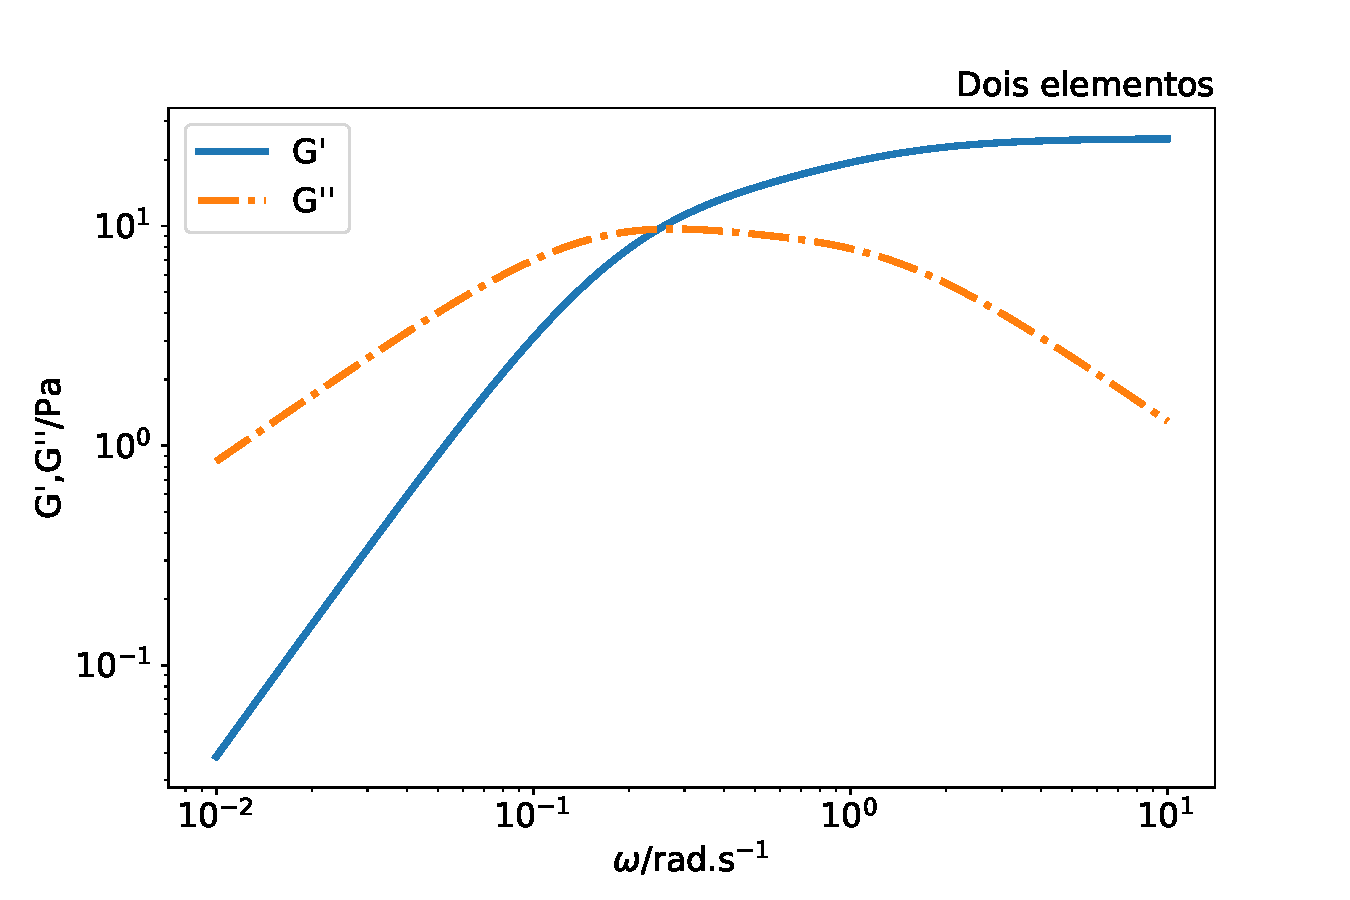
\includegraphics[width=\textwidth]{./imagens/reologia/modelos_comparativo_doismodos}
					\caption{Dois Módulos. \(G_1=10, G=15, \tau_{\textrm{rel,1}}=1,  \tau_{\textrm{rel,2}}=5\)}
					\label{fig:comparativo_modelo_doismodos}
				\end{subfigure}
			
				\begin{subfigure}[t]{.5\textwidth}
					\centering
					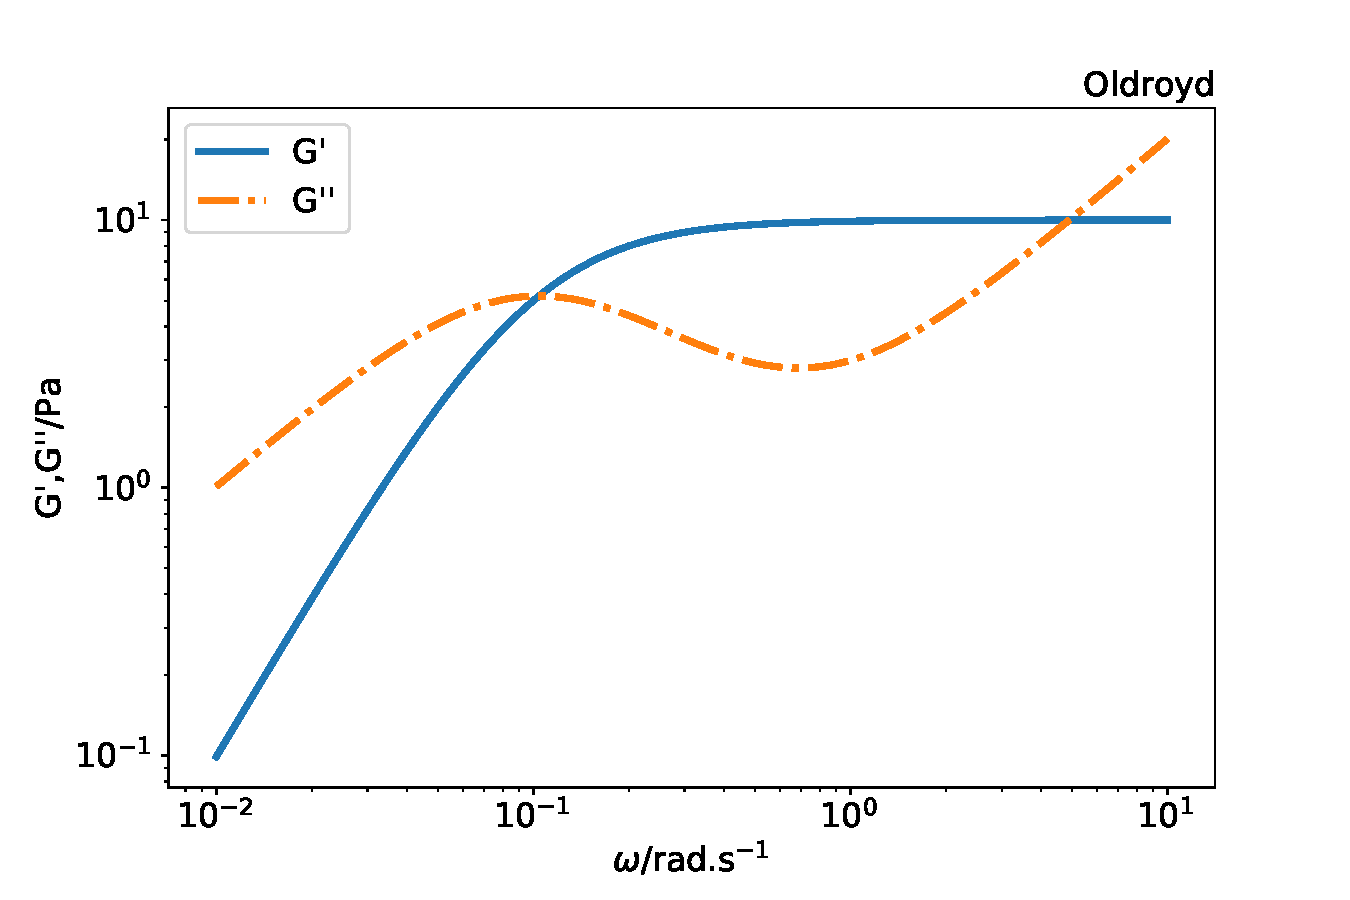
\includegraphics[width=\textwidth]{./imagens/reologia/modelos_comparativo_oldroyd}
					\caption{Oldroyd. \(G=10, \tau_{\textrm{rel}}=10, \eta_{\infty}=2\)}
					\label{fig:comparativo_modelo_oldroyd}
				\end{subfigure}%	
				\begin{subfigure}[t]{.5\textwidth}
					\centering
					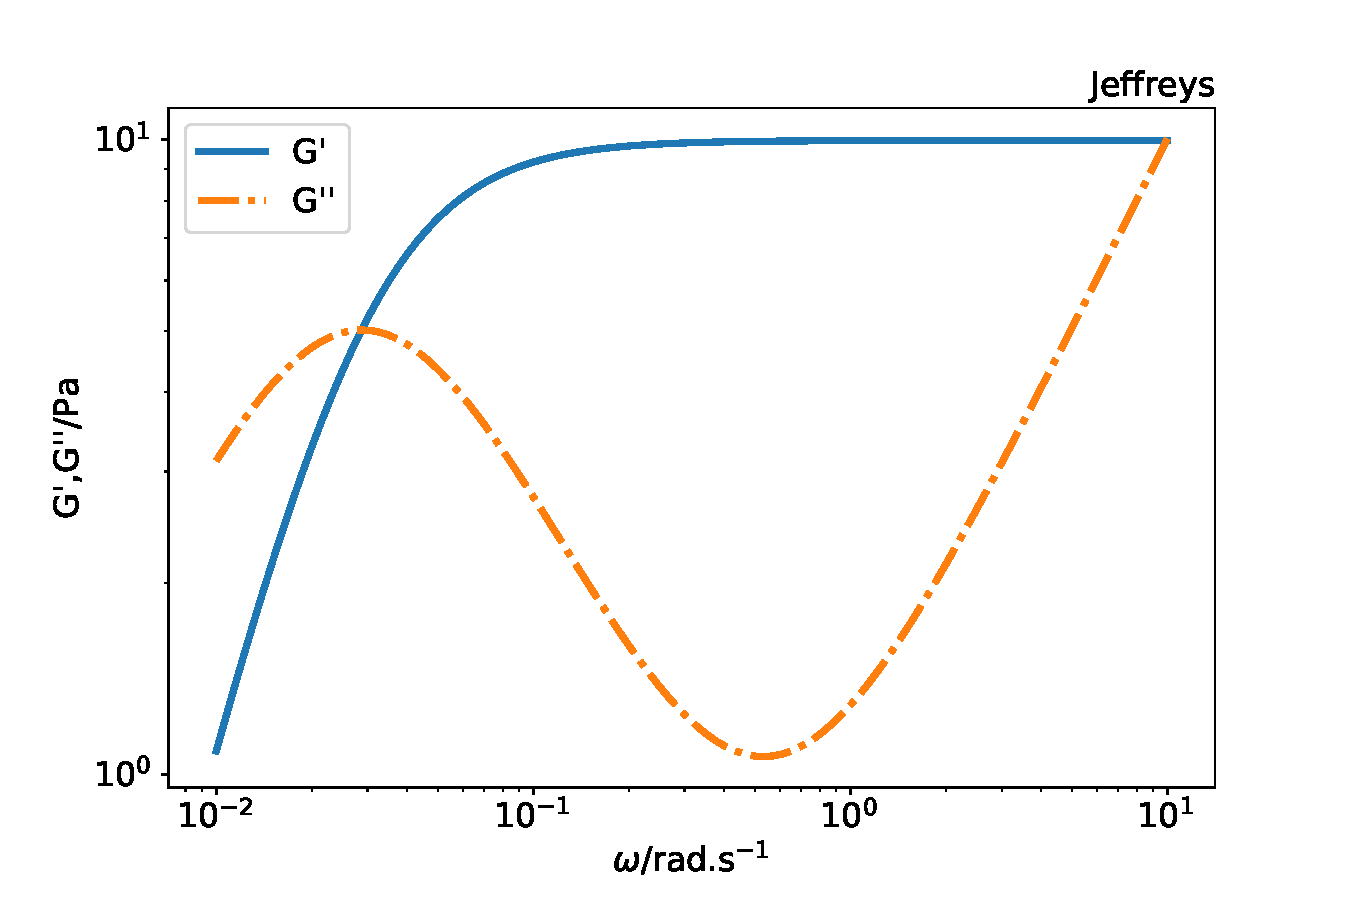
\includegraphics[width=\textwidth]{./imagens/reologia/modelos_comparativo_jeffreys}
					\caption{Jeffreys. \(G=10, \tau_{\textrm{rel,1}}=35, \tau_{\textrm{rel,2}}=0.1 \)}
					\label{fig:comparativo_modelo_jeffreys}
				\end{subfigure}
			
				\caption{Comparação dos modelos de Maxwell, Dois-Módulos, Oldroyd e Jeffreys. Nas legendas estão os parâmetros para a criação dos modelos. Os módulos estão na unidade de Pa, os tempos de relaxação, em \(s.rad^{-1}\) e \(\eta_{\infty}\) em Pa.s}
				\label{fig:comparativo_modelos}
			\end{figure}
			
			% todo: pensar se eu devo descrever os detalhes de micelas gigantes aqui, ou na seção de micelas mesmo.
			% todo: colocar o modelo de García-Saraji
	\chapter{Calorimetria de titulação isotérmica}
	
		\section{Fundamentos}
		
		% todo: encontrar um termo melhor para ``caixa adiabática''
		
		A calorimetria de titulação isotérmica (ITC) é uma técnica baseada num processo de titulação, onde cada injeção resulta em uma ou mais reações químicas ou físicas que podem liberar ou absorver calor. O calor total observado é a somatória de todos os processos que ocorreram durante a injeção. No calorímetro há duas celas dentro de uma caixa adiabática, uma de referência, que contém somente água, e outra de amostra, onde ocorre a titulação em si. A cela de referência recebe uma quantidade fixa de calor através de uma resistência, e a cela de amostra recebe uma quantidade variável de calor. Isso significa que a temperatura das celas, no decorrer de uma titulação, aumenta ligeiramente, mas menos que 0,1°C. A figura \ref{fig:ITC_esquema} ilustra a construção de um calorímetro.
		
		\begin{figure}[h]
			\centering
			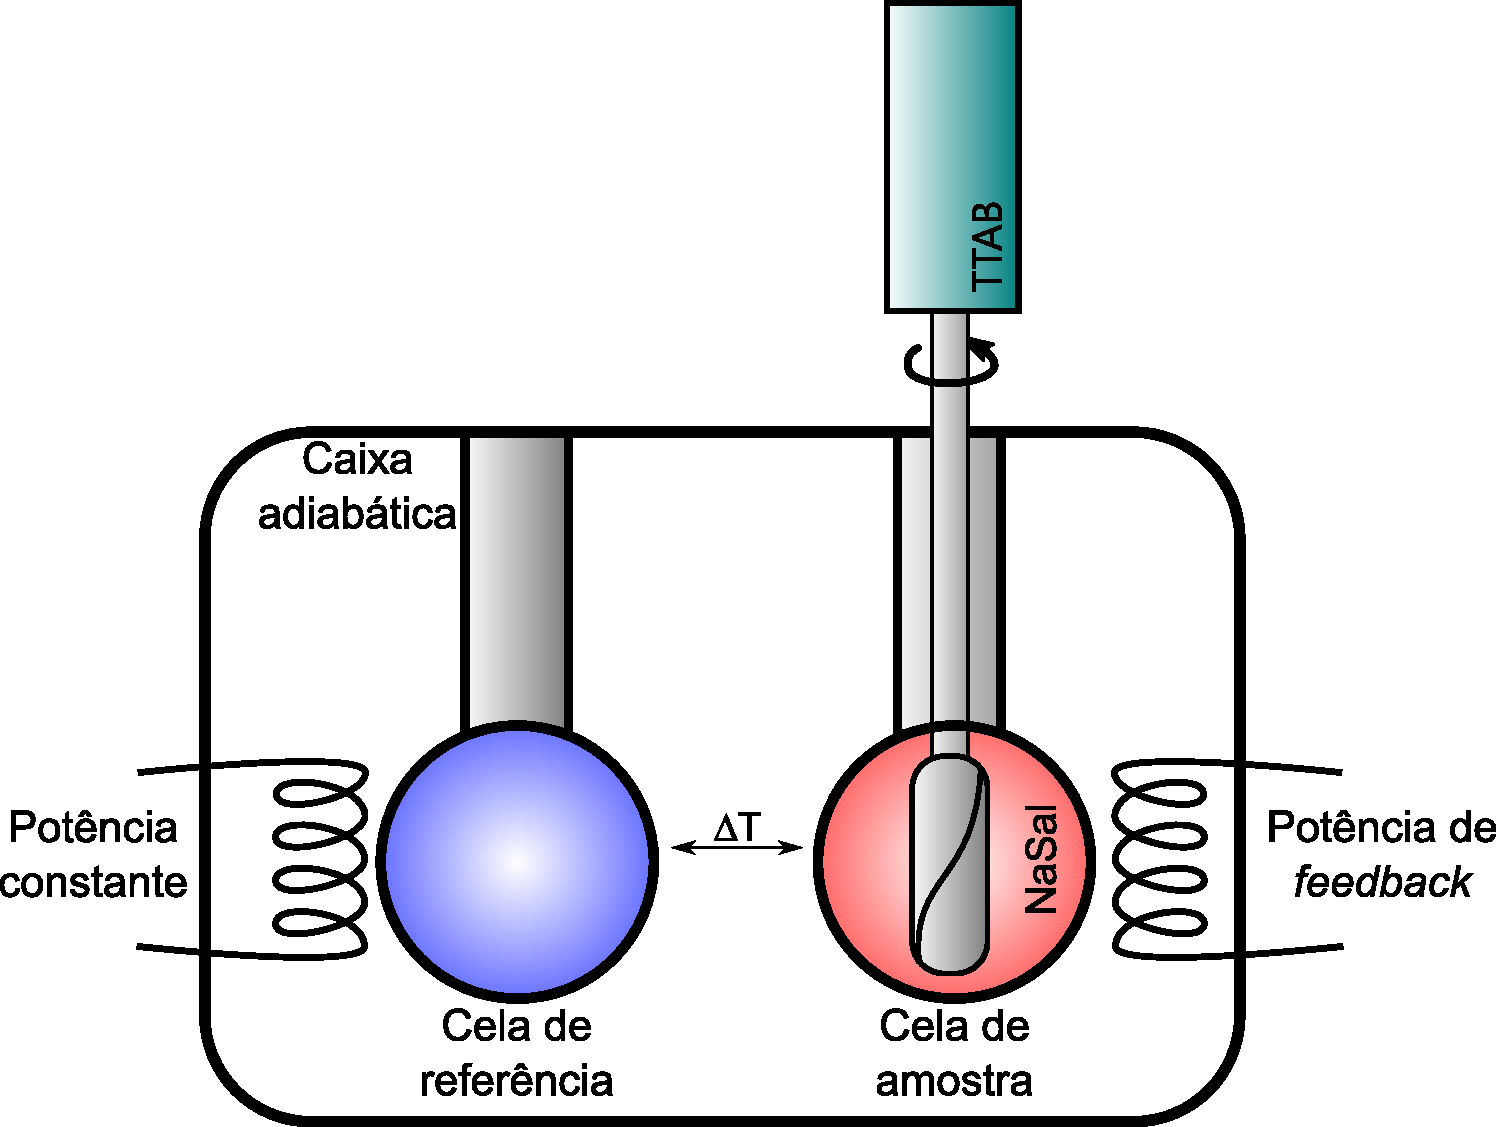
\includegraphics[width=0.5\textwidth]{./imagens/itc/esquema_itc_equipamento}
			\caption{Esquema da construção de um calorímetro de titulação isotérmica}
			\label{fig:ITC_esquema}
		\end{figure}
		
		Durante uma titulação, caso ocorra liberação de calor na cela de amostra, menos energia, em relação ao valor basal, precisa ser fornecida para manter a temperatura igual entre as celas. Caso o sistema absorva energia, mais potência precisa ser fornecida à cela. Esse comportamento se expressa em picos acima ou abaixo da linha de base. A integração de cada pico no tempo fornece valores de energia que, quando divididos pelo número de mols injetados, obtemos valores de $\Delta H^0/kJ.mol^{-1}$ [X, Y]. A figura \ref{fig:ITC_exemplo} mostra um exemplo de um experimento de titulação de \TTAB{} em água.
		
		\begin{figure}[h]
			\begin{subfigure}[t]{0.5\textwidth}
				\centering
				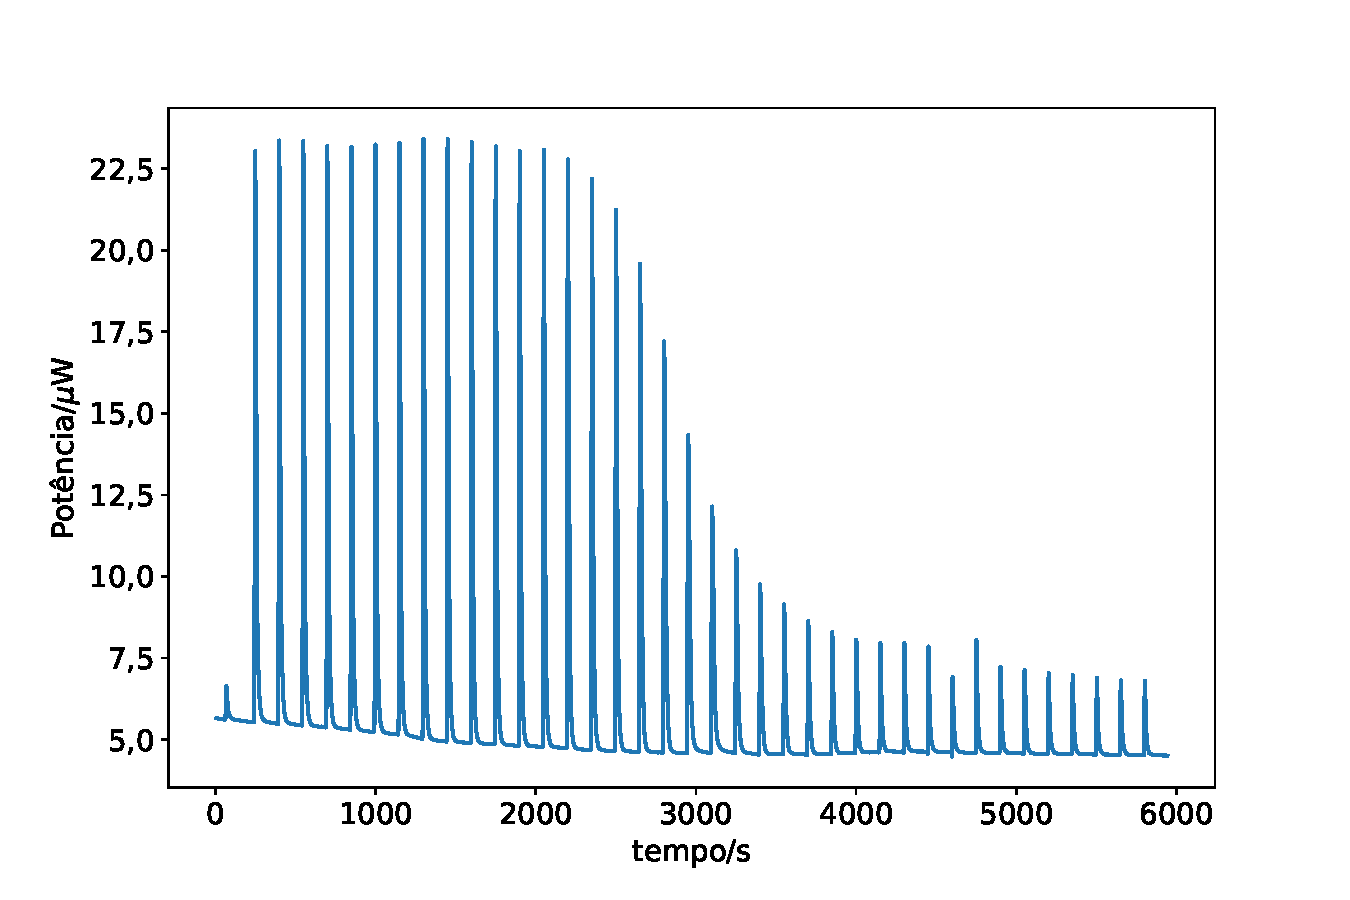
\includegraphics[width=\textwidth]{./imagens/itc/raw_itc_exemplo}
				\caption{Dado bruto}
				\label{fig:ITC_raw_exemplo}
			\end{subfigure}%
			\begin{subfigure}[t]{0.5\textwidth}
				\centering
				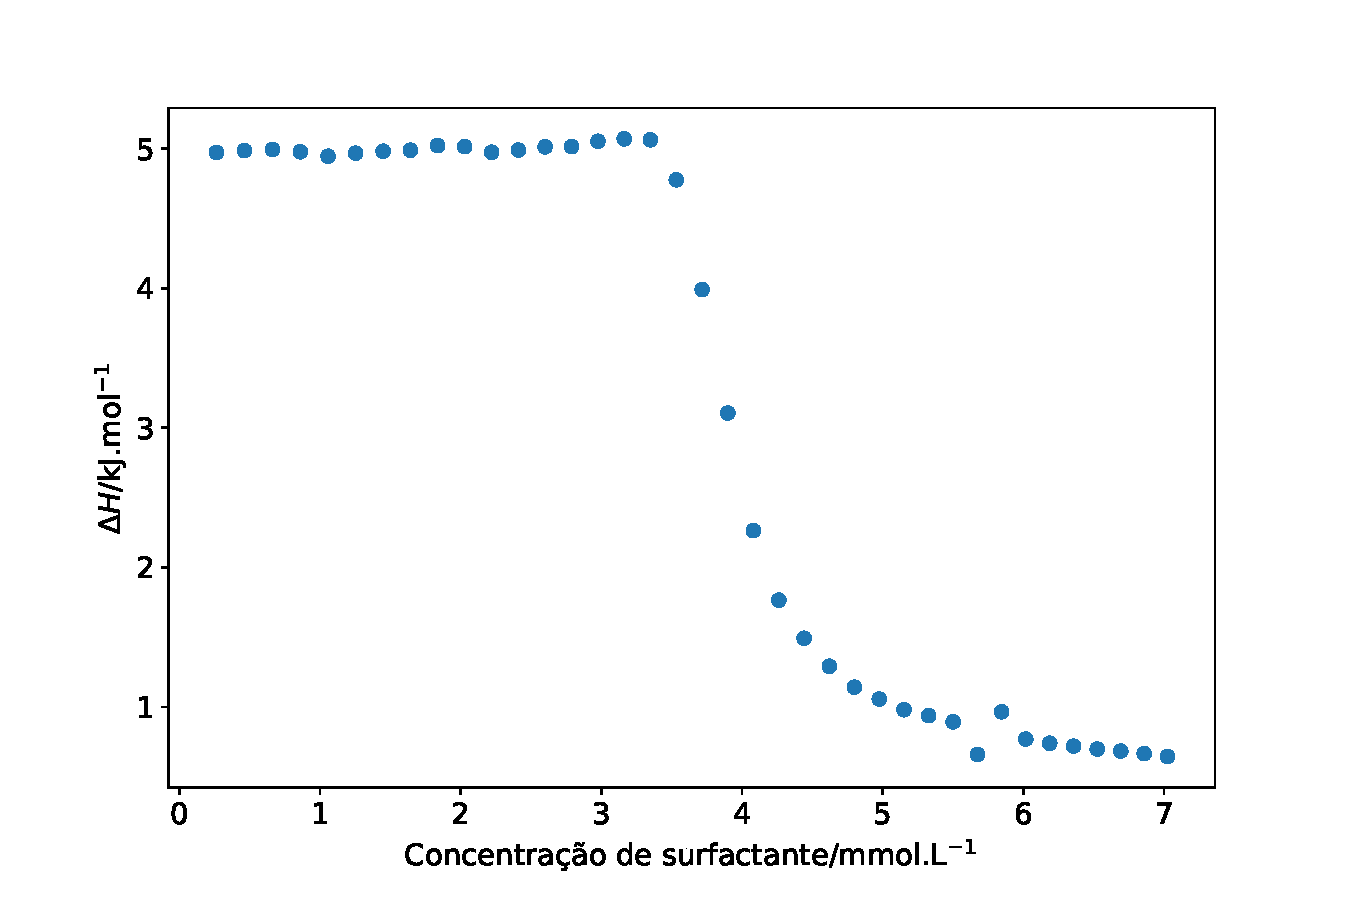
\includegraphics[width=\textwidth]{./imagens/itc/inj_itc_exemplo}
				\caption{Entalpograma}
				\label{fig:ITC_inj_exemplo}
			\end{subfigure}
		
			\caption{Titulação de \TTAB{} 42 \mM{} em água, mostrando o calor absorvido pela célula durante a titulação (\ref{fig:ITC_raw_exemplo}). A primeira injeção é descartada para garantir que as injeções subsequentes possuam um volume correto de injeção. A integração dos picos em relação à linha base, dividindo-se isso pela concentração de surfactante injetado, resulta no entalpograma (\ref{fig:ITC_inj_exemplo})}
			\label{fig:ITC_exemplo}
		\end{figure}
		
		\section{Calorimetria de micelização}
		
		A partir de um conjunto de dados como os da figura \ref{fig:ITC_exemplo}, é possível calcular a \cmc{} e a entalpia de micelização, \DHmic. A \cmc{} é determinada pelo ponto de inflexão, onde a primeira derivada do entalpograma é maior (ou menor). A \DHmic{} é determinada realizando-se dois ajustes lineares das regiões iniciais e finais do entalpograma. A diferença de entalpia dos pontos de intersecção desses ajustes com uma reta horizontal na \cmc{} fornece o \DHmic{} sem correção. Após isso, é necessário corrigir pela concentração de surfactante não micelizado na seringa, que é igual à \cmc{}. A figura \ref{fig:itc_extracao_cmc_dh} mostra esse método.
		
		\begin{figure}[h]
			\centering
			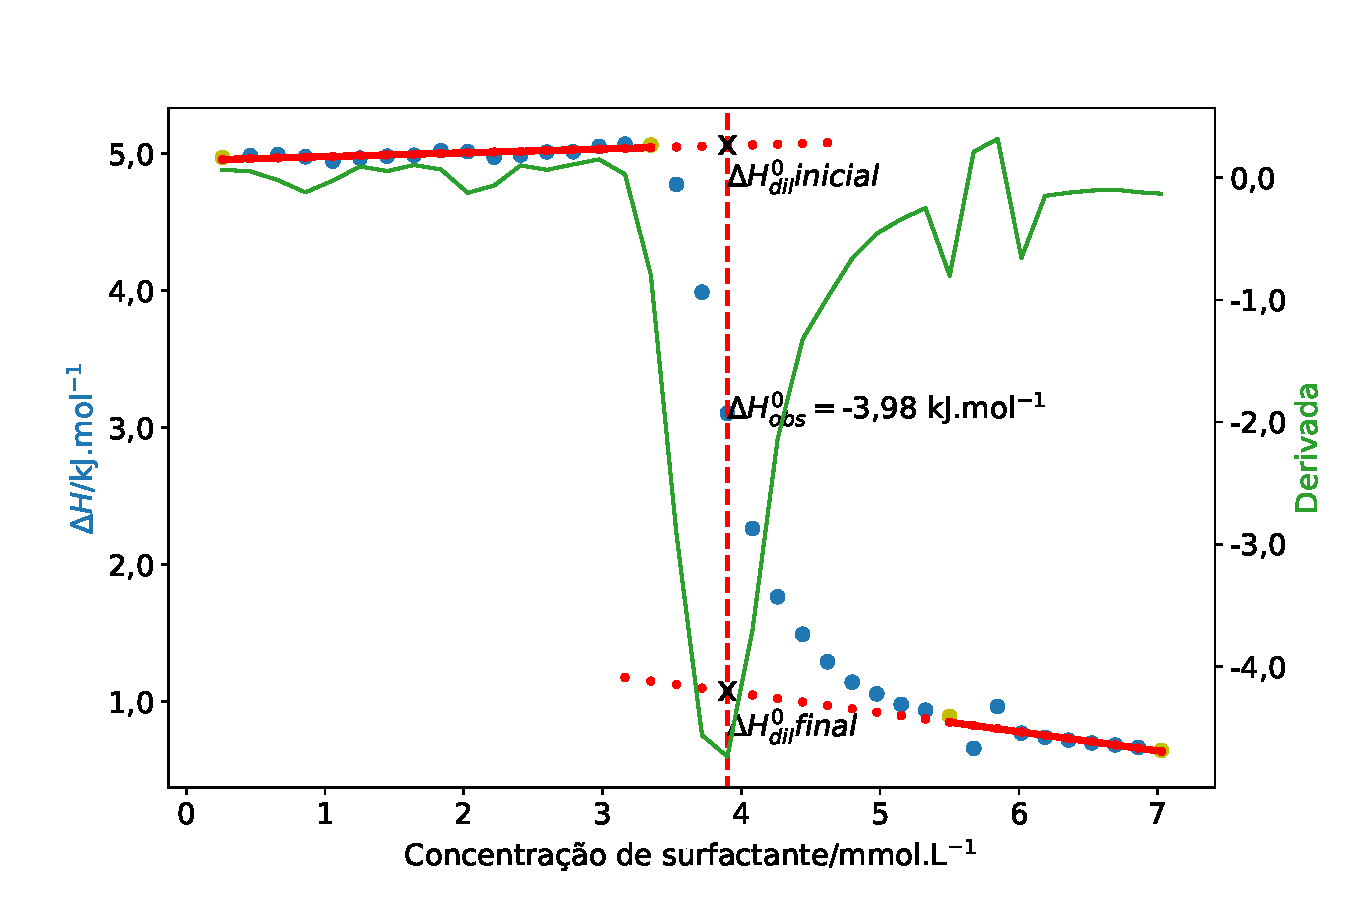
\includegraphics[width=0.7\textwidth]{imagens/itc/extracao_cmc_dh_exemplo}
			\caption{Método para extração da concentração micelar crítica (\cmc) e a entalpia de micelização \DHmic. A curva em verde é a derivada do entalpograma. Os pontos amarelos limitam as regiões onde são feitos ajustes lineares. A }
			\label{fig:itc_extracao_cmc_dh}
		\end{figure}  % todo: checar se as unidades estão corretas

		Para corrigir a entalpia de micelização observada para obter a entalpia de micelização correta, utiliza-se a equação \ref{eqn:itc_obtencao_dhmic}. 
		
		\begin{equation}
			\Delta H^0_{\textrm{mic}} = \Delta H^0_{\textrm{obs}} \times \dfrac{c_{\textrm{seringa}}}{c_{\textrm{seringa}-\textrm{cmc}}}
			\label{eqn:itc_obtencao_dhmic}
		\end{equation}  % todo: ficar de olho aqui porque tem termos que não estão em macros e precisam ser revistos quando algo mudar
		
		\noindent onde \(c_{\textrm{seringa}}\) é a concentração de surfactante na seringa.
		
		Pela \cmc{} é possível obter a energia livre de micelização a partir da equação \ref{eqn:itc_DeltaG_mic}, dependendo do tipo de surfactante e do meio.
		
		\begin{equation}
			\Delta G_{\textrm{mic}}^0
			\begin{cases}
			= RT\ln(\chi_{\textrm{cmc}})      & \textrm{Surfactante não iônico}      \\
			= (2-\alpha)RT\ln(\chi_{\textrm{cmc}}) & \textrm{Surfactante iônico}					\\
			\end{cases}
			\label{eqn:itc_DeltaG_mic}
		\end{equation}
		
		\noindent onde \(\alpha\) é o grau de ionização das micelas e \(\chi_{\textrm{cmc}}\) é a concentração micelar crítica em fração molar. O cálculo para surfactantes iônicos assume que o solvente é água e/ou a força iônica seja baixa.
		
		Com a entalpia e energia livre de micelização, é possível encontrar a entropia de micelização pela equação de Gibbs (Eq. \ref{eqn:itc_gibbs_para_entropia}).
		
		\begin{equation}
			T\Delta S^0_{\textrm{mic}} = \Delta H^0_{\textrm{mic}} - \Delta G^0_{\textrm{mic}}
			\label{eqn:itc_gibbs_para_entropia}
		\end{equation}

		% todo: olhar a dissertação do césar para ver algumas dicas e para colocar alguns termos. Tem bastante coisa boa lá.

	\chapter{SAXS}
		\section{Fundamentos}
				
		%O espalhamento de luz é um fenômeno que ocorre devido à interação da luz com os elétrons de um átomo ou grupo de átomos. O feixe incidente excita os elétrons de modo que eles comecem a oscilar na mesma frequência do feixe incidente. Quando o feixe incidente é removido, os elétrons excitados emitem fótons do mesmo comprimento de onda incidente (chamado de espalhamento elástico), em qualquer direção. As ondas emitidas interagem de maneira construtiva e destrutiva, dependendo de sua posição relativa. A somatória dessas ondas resulta num padrão de espalhamento específico para cada estrutura.
		
		A radiação eletromagnética, quando incide sobre uma amostra fina, o campo elétrico variante da radiação irá interagir com os elétrons dos átomos dentro da região iluminada. Dependendo da frequência (\(\omega\)), pode ocorrer o fenômeno da absorção perto do limite de Lorentz, \(\omega \approx \omega_0\), de interesse em experimentos espectroscópicos, ou pode ocorrer uma polarização dos átomos que varia com a frequência da radiação quando \(\omega \ll \omega_0\) ou \(\omega \gg \omega_0\). Os dipolos emitem radiação pois toda carga elétrica emite um campo elétrico em direções praticamente aleatórias, com amplitude proporcional à aceleração. Isso é chamado de espalhamento. Essas ondas espalhadas interagem construtiva- e destrutivamente, originando em padrões de espalhamento dependendo da localização dos centros espalhadores.
		
		Raios-X possuem comprimentos de onda tão pequenos que se encontram no limite de Thomson, onde \(\omega \gg \omega_0\). No campo da matéria mole, a energia dos fótons é tão alta que todos os elétrons dos átomos, até suas camadas mais internas, oscilam junto com a radiação. Isso não acontece com o espalhamento de luz, onde a oscilação ocorre somente com os elétrons das camadas mais externas, dependendo da polarizabilidade dos átomos, que é proporcional ao índice de refração do material. % todo: pensar se eu coloco aqui a fórmula
		
		As ondas emitidas, quando comparadas com o feixe incidente, são coerentes, isso é, possuem somente uma diferença de fase \(\varphi\) fixa entre a radiação incidente e espalhada, e possuem o mesmo comprimento de onda da radiação incidente, isso é, o espalhamento é completamente elástico. Dessa maneira, os vetores incidentes \(\mathbf{k_i}\) e espalhados \(\mathbf{k_s}\) possuem a mesma amplitude, igual ao número de onda \(k\) (Eq. \ref{eqn:numero_onda}), com o índice de refração próximo à unidade.
		
		\begin{equation}
			k = \dfrac{2 \pi}{\lambda}
			\label{eqn:numero_onda}
		\end{equation}
		
		\noindent onde \(\lambda\) é o comprimento de onda da radiação.
		
		A única diferença entre os feixes espalhados é a fase \(\varphi\) da radiação, devido ao caminho diferente que cada feixe precisa fazer. A diferença de fase de um comprimento de onda é \(2\pi\). Essa fase está relacionada com a interferência dos feixes e, para obtê-la, é necessário subtrair os vetores incidente e espalhado, que passam por um ponto \(P\), cuja posição é dada pelo vetor \(\mathbf{r}\), multiplicados pelo número de onda \(k\) (Eq. \ref{eqn:calculo_fase_saxs}):
		
		\begin{equation}
			\varphi = - \left( \dfrac{2\pi}{\lambda} \right) \mathbf{r} \cdot \left( \mathbf{k_s} - \mathbf{k_i} \right)
			\label{eqn:calculo_fase_saxs}
		\end{equation}
		
		O sinal negativo na equação \ref{eqn:calculo_fase_saxs} é devido à inversão da ordem de subtração dos vetores \(\mathbf{k_i}\) e \(\mathbf{k_s}\). Assim, podemos introduzir o vetor de espalhamento \(\mathbf{q}\), também conhecido como vetor de transferência de momento (Eq. \ref{eqn:vetor_espalhamento}).
		
		\begin{equation}
			\mathbf{q} = \left( \dfrac{2\pi}{\lambda} \right) \mathbf{r} \cdot \left( \mathbf{k_s} - \mathbf{k_i} \right)
			\label{eqn:vetor_espalhamento}
		\end{equation}
		
		Logo, a defasagem pode ser facilmente relacionada com a posição dos centros espalhadores e o vetor de espalhamento:
		
		\begin{equation}
			\varphi = - \mathbf{q} \cdot \mathbf{r}
			\label{eqn:defasagem_qr}
		\end{equation}
		
		Uma consequência do produto escalar da equação \ref{eqn:defasagem_qr} é que somente a componente de \(\mathbf{r}\) na direção de \(\mathbf{q}\) é relevante para a fase \(\varphi\). Isso implica que todos os pontos num plano perpendicular a \(\mathbf{q}\) possuirão a mesma fase. Isso dá origem à ideia de que o espalhamento ocorre como uma reflexão da radiação por um conjunto de planos, comumente utilizado em cristalografia.
		
		A amplitude do vetor de espalhamento é dado pela eq. \ref{eqn:amplitude_vetor_espalhamento}, onde \(\theta\) é o ângulo de espalhamento, entre os vetores \(\mathbf{k_i}\) e \(\mathbf{k_s}\).
		
		\begin{equation}
		q = \dfrac{4\pi}{\lambda} \sin\left(\dfrac{\theta}{2}\right)
		\label{eqn:amplitude_vetor_espalhamento}
		\end{equation}
		
		A figura \ref{fig:esquema_saxs} ilustra os vetores incidente e espalhado, assim como o cálculo do vetor.
		
		\begin{figure}[h]
			\centering
			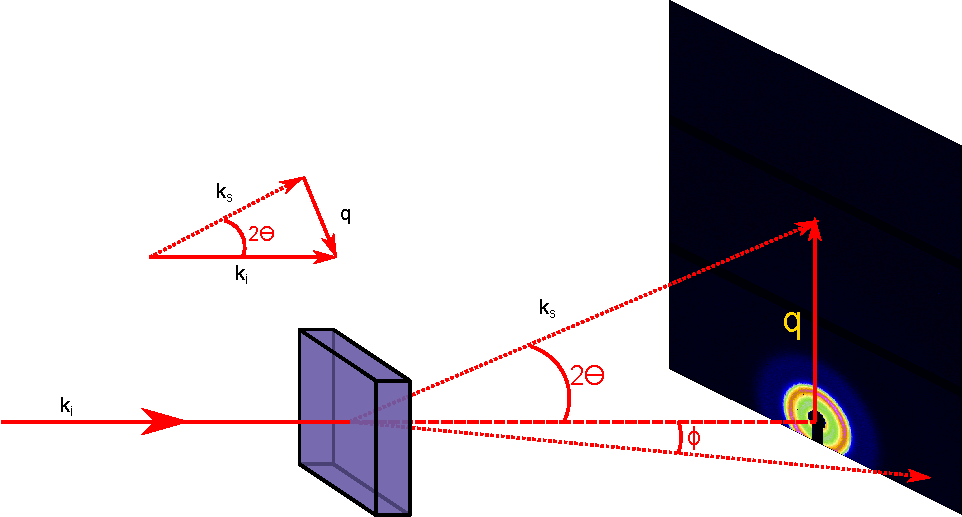
\includegraphics[width=0.7\textwidth]{imagens/saxs/Esquema_SAXS}
			\caption{Diagrama mostrando o feixe incidente de raios-X sendo espalhado por um material, resultando num vetor espalhado. O vetor de espalhamento, \(\mathbf{q}\) é paralelo à subtração vetorial dos vetores \( \mathbf{k_i} \) e \( \mathbf{k_s} \), paralelos à direção dos feixes incidente e espalhado. Os feixes, após interagirem, atingem o detector, e a imagem resultante é composta pela contagem de fótons em cada pixel. O ponto escuro é resultante do bloqueio da radiação não espalhada pelo \emph{beam-stop}.}
			\label{fig:esquema_saxs}
		\end{figure}
		
		Para pequenos valores de \(\sfrac{\theta}{2}\), \(\sin(\sfrac{\theta}{2}) \approx \sfrac{\theta}{2}\), então a magnitude do vetor de espalhamento \(\mathbf{q}\) (que será chamado de \q{} de agora em diante) é proporcional ao ângulo de espalhamento (em radianos). A unidade do vetor de espalhamento é tipicamente \(nm^{-1}\), dependendo claro do comprimento de onda utilizado. Uma grande utilidade de se utilizar o vetor de onda é que o espalhamento se torna independente da fonte de radiação, pois o comprimento de onda já é levado em consideração. Além disso, o inverso de \q{} informa o tamanho dos objetos que geralmente são observados em SAXS. Faixas comuns são de 0,006 a 6 \(nm^{-1}\), o que resulta em estruturas da faixa de 1\(\mu m\) a 1 \(nm\).

		Para se determinar o padrão obtido na figura \ref{fig:esquema_saxs}, é necessário somar todas as ondas espalhadas em cada uma das posições. A função de onda genérica para uma das ondas espalhadas é dada pela Eq. \ref{eqn:funcao_onda_espalhamento}.%, onde \(\mathbf{r}\) é o vetor de posição na partícula.
		
		\begin{equation}
			\psi(\mathbf{q}) = \exp(-i \mathbf{q} \cdot \mathbf{r})
			\label{eqn:funcao_onda_espalhamento}
		\end{equation}
		
		A somatória das funções de onda, Eq. \ref{eqn:SAXS_somatoria_contribs}, resulta na amplitude de espalhamento. O termo \(b_j\) é o comprimento de espalhamento de cada ponto. Para elétrons, seu comprimento de espalhamento é o raio do elétron, \(r_e = 0.2817 \times 10^{-12}\) cm.
		
		\begin{equation}
			A(\mathbf{q}) = \sum_j b_j \exp(-i \mathbf{q} \cdot \mathbf{r})
			\label{eqn:SAXS_somatoria_contribs}
		\end{equation}
		
		Porém, a resolução de raios-X geralmente não permite a observação dos elétrons individuais, então a somatória dos comprimentos de espalhamento de todos os elétrons no átomo, dividido pelo seu volume, resulta na densidade de comprimento de espalhamento \(\rho\) (Eq. \ref{eqn:SLD}). Esse termo também é conhecido como SLD, do inglês \emph{scattering length density}.
		
		\begin{equation}
			\rho(\mathbf{r}) = \sum_j \dfrac{b_j}{v}
			\label{eqn:SLD}
		\end{equation}
		
		Se a densidade for uniforme, podemos encontrar a densidade a partir da fórmula estrutural do material:
		
		\begin{equation}
			\rho = \dfrac{n_e d_M N_a}{M_w} r_e
			\label{eqn:rho_uniforme}
		\end{equation}
		
		\noindent onde \(n_e\) é o número de elétrons do material, \(d_M\) é sua densidade (água é 1000 kg/m\textsuperscript{3}), \(N_a\) é o número de Avogadro, \(M_w\) é a massa molar do material e \(r_e\) é o raio do elétron.
		
		Assim, a eq. \ref{eqn:SAXS_somatoria_contribs} passa de uma somatória para uma integral, eq. \ref{eqn:SAXS_integral_amplitude}.
		
		\begin{equation}
			A(\mathbf{q}) = \int_V \rho(\mathbf{r}) \exp(-i \mathbf{q} \cdot \mathbf{r}) d\mathbf{r}
			\label{eqn:SAXS_integral_amplitude}
		\end{equation}
		
		A intensidade de espalhamento, detectada pelo equipamento, é obtida pela média pelo tempo de todas as posições e conformações possíveis das partículas, ao quadrado (multiplicando-se pelo complexo conjugado). É necessário utilizar constantes para normalizar essa intensidade, como o número \(n\) de partículas espalhadoras e o volume \(V\) das partículas. Além disso, como as partículas estão num meio, como um solvente, é necessário considerar a densidade eletrônica do solvente, e por isso utiliza-se \(\Delta \rho^2\), a diferença entre a densidade do solvente e do meio, também conhecido como contraste. Tudas essas considerações resultam na equação \ref{eqn:SAXS_I_funcao_A}.
		
		\begin{equation}
		I(q) = n\Delta \rho^2 V^2 |A(q)|^2
		\label{eqn:SAXS_I_funcao_A}
		\end{equation}
		
		Sistemas com alto contraste, por exemplo, partículas de ouro em água, espalham bastante raios-X, resultando em sinais de boa qualidade. Porém sistemas de baixo contraste, como a maior parte de sistemas de materia mole, incluindo o sistema \CTAB{} + NaSal, utilizado neste trabalho, não resultam em uma boa resolução sinal/ruído. Tipicamente, o contraste das cabeças é positivo em relação à água, mas o contraste das cadeias é negativo, o que resulta num contraste total baixo. Logo, é interessante calcular o contraste, o que pode ser feito por programas como o SASfit.\footnote{\url{https://github.com/SASfit/SASfit}}. Algumas vezes é possível melhorar o contraste adicionando-se sacarose ou glicerina ao solvente ao meio, porém isso só é válido para experimentos de SAXS, não de espalhamento de luz.
		
		\section{Modelagem e o problema inverso do espalhamento}
		
		O objetivo de análises de SAXS é obter informações estruturais das partículas presentes no meio. Esse é chamado o problema inverso do espalhamento, em contraste com o problema direto, onde estruturas são propostas e o padrão de espalhamento das mesmas é calculado. Para resolver o problema inverso, é necessário primeiramente obter os modelos necessários, um processo matematicamente bastante complexo, e depois ajustá-los às curvas obtidas, variando-se os parâmetros de ajuste pelo método dos mínimos quadrados. A etapa de ajuste também possui seu grau de dificuldade, necessitando frequentemente de técnicas complementares para a escolha de um modelo e para fornecer chutes iniciais para os parâmetros.
		
		\subsection{Partículas esféricas homogêneas em solução}
		
		Quando se considera o espalhamento de um único objeto não centro-simétrico, é necessário considerar a orientação do vetor de espalhamento \q{} para obter o padrão de espalhamento. Além disso, em solução, esses objetos estão possivelmente orientados aleatoriamente, sendo necessário realizar uma integração sobre todas as orientações possíveis. Porém, objetos centro-simétricos, como esferas de raio \(R\), não necessitam disso, e a amplitude de espalhamento pode ser calculada pela eq. \ref{eqn:SAXS_amplitude_esfera}. % Note que foi utilizada a relação de Euler.
		
		\begin{equation}
			A(q) = \dfrac{4\pi\Delta\rho}{q} \int_0^R r\sin(qr) dr
			\label{eqn:SAXS_amplitude_esfera}
		\end{equation}
				
		Realizando uma integração parcial, obtemos:
		
		\begin{equation}
			A(q) = \Delta_\rho \dfrac{4\pi R^3}{3} \left[ \dfrac{3 \left( \sin qR - qR \cos qR \right)}{\left(qR\right)^3} \right]
			\label{eqn:SAXS_amplitude_esfera_integrado}
		\end{equation}
		
		Essa equação, normalizada, é utilizada na descrição do modelo de micelas gigantes (Eq. \ref{eqn:AP_Fsphere}) que está presente no apêndice \ref{sec:modelo_MG_matematica}.
		
		Como a intensidade de luz espalhada é o quadrado da amplitude:
		
		\begin{equation}
			I(q) = (\Delta \rho)^2 V^2 P_0=(\Delta \rho)^2 V^2 \left[ \dfrac{3 \left( \sin qR - qR \cos qR \right)}{\left( qR \right) ^3} \right]
			\label{eqn:SAXS_intensidade_esfera}
		\end{equation}
		
		O termo à direita da equação \ref{eqn:SAXS_intensidade_esfera} é chamado de fator forma normalizado, \(P_0\). Esse fator forma possui vários mínimos em valores de \(qR\) em 4,493, 7,725, etc (figura \ref{fig:espalhamento_esfera}). A partir desses mínimos é possível obter o raio da partícula, apesar de que isso só é válido para partículas monodispersas, totalmente esféricas, homogêneas e em uma solução diluída.
		
		\begin{figure}[h]
			\centering
			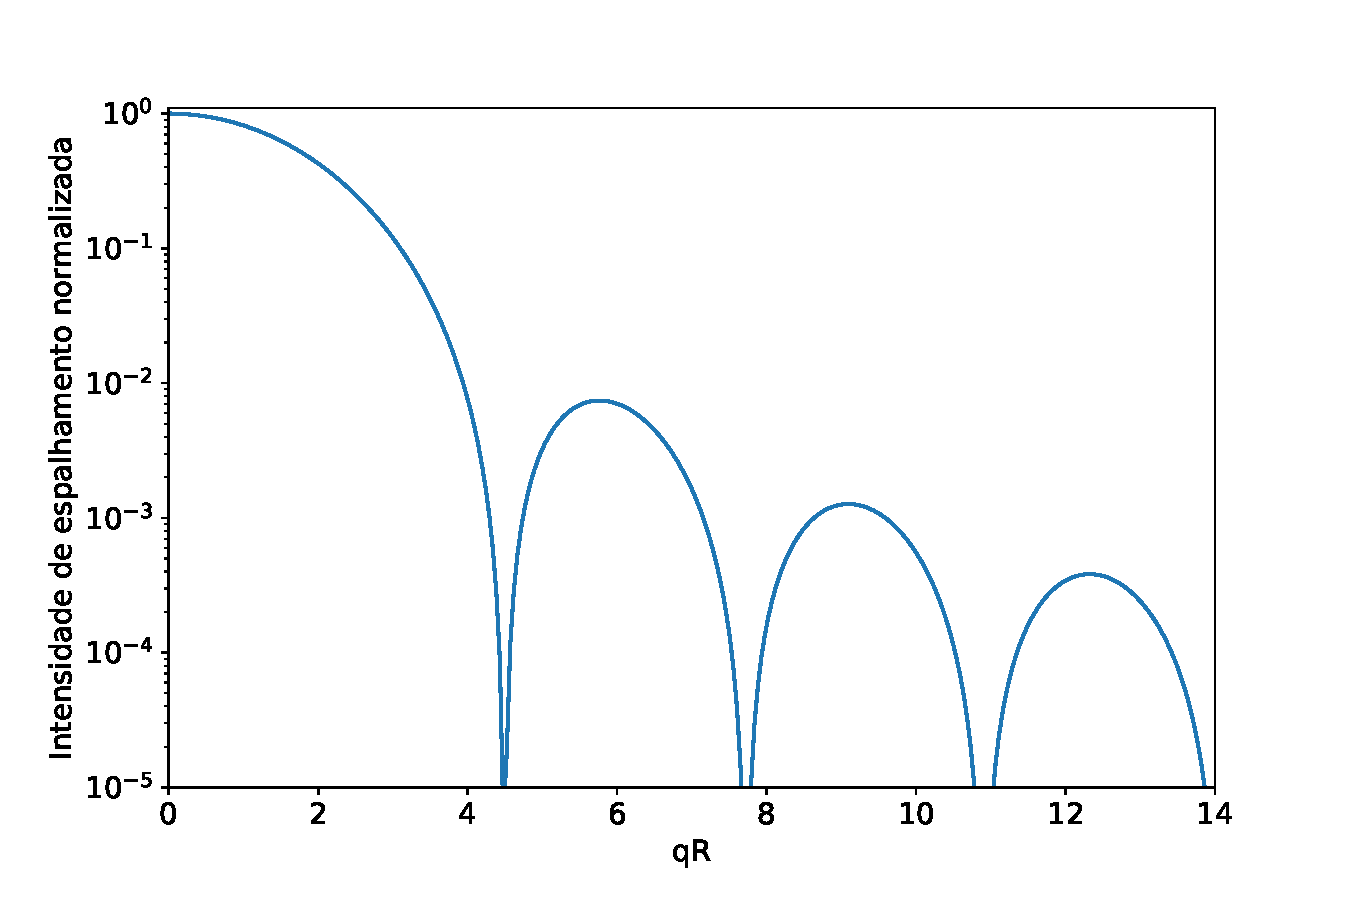
\includegraphics[width=0.7\textwidth]{imagens/saxs/espalhamento_esfera_monodispersa}
			\caption{Espalhamento de uma esfera monodispersa. Os mínimos estão relacionados com o raio da esfera. O código para fazer este gráfico se encontra na listagem \ref{lst:plot_micela_esferica}.}
			\label{fig:espalhamento_esfera}
		\end{figure}
		
		\begin{listing}[H]
			\inputminted{python}{./python/plot_saxs_esfera.py}
			\caption{Código utilizado para a criação da figura \ref{fig:espalhamento_esfera}}
			\label{lst:plot_micela_esferica}
		\end{listing}
		
		Esse é o exemplo mais simples para a derivação da amplitude de espalhamento de um objeto. Quanto maior for a complexidade dos objetos modelados, e mais concentrada for a solução, mais difícil fica a derivação dos modelos, exigindo considerável experiência e conhecimento matemático. O Prof. Jan Skov Pedersen, da Dinamarca, adaptou modelos descritos na literatura para descrever sistemas alongados em solução, como polímeros e micelas gigantes. Uma descrição matemática superficial do modelo desenvolvido se encontra na no apêndice, seção \ref{sec:modelo_MG_matematica}, e uma adaptação desse modelo na linguagem Python se encontra na seção \ref{sec:modelo_MG_python}.
		
		\subsection{Fator estrutura, concentrações altas}
		
		Quando a translação e orientação de uma partícula em solução começa a depender das outras, uma contribuição do espalhamento dessas correlações começa a se tornar visível. Esse fator adicional, chamado de fator estrutura, \(S(q)\), deve ser multiplicado ao \(P(q)\) para se obter o valor da intensidade correta (Eq. \ref{eqn:SAXS_I_P_S}). Em soluções diluídas, a contribuição do fator estrutura se cancela devido à posição e orientação arbitrárias das partículas, então \(S(q) \approx 1\).
		
		\begin{equation}
			I(q) = n\Delta \rho^2 V^2 P(q) S(q)
			\label{eqn:SAXS_I_P_S}
		\end{equation}
		
		% todo: pensar se eu devo colocar uma parte de mínimos quadrados, mostrando exemplo com código, ou Excel também.
		Como as distâncias entre partículas são tipicamente maiores do que as distâncias dentro das partículas, as contribuições do fator estrutura geralmente aparecem com maior intensidade em valores de \q{} baixos.
		
		Existem vários modelos possíveis para o fator \(S(q)\), que dependem de uma função que descreve a probabilidade de se encontrar uma partícula a uma distância \(r\) de outra. Dentro dessa função, existe um potencial que pode descrever, por exemplo, se há atração ou repulsão eletrostática entre as partículas. O modelo das esferas rígidas sem carga, o mais simples, que possui o seguinte potencial (Eq. \ref{eqn:potencial_esfera_rígida}):
		
		\begin{equation}
			u(r) = 
			\begin{cases}
				\infty  & r < (R_a + R_b) \\
				0		& r > (R_a + R_b)
			\end{cases}
			\label{eqn:potencial_esfera_rígida}
		\end{equation}

		\noindent onde \(R_a\) e \(R_b\) são os raios de duas partículas que estão interagindo.
		
		A presença de fatores estrutura adicionam alguns parâmetros fortemente não lineares ao ajuste e aumentam grandemente a complexidade dos mesmos, tornando a determinação do fator forma e estrutura simultaneamente uma tarefa bastante difícil. Além disso, quando há polidispersidade nos sistemas, não se torna possível a completa separação dos termos \(P(q)\) e \(S(q)\) (como é o caso das micelas gigantes do apêndice \ref{sec:modelo_MG_matematica}) e é necessário utilizar um fator estrutura efetivo, \(S_m(q)\).
		
		\subsection{Indexação de picos}
		\label{sec:teoria_SAXS}
		
		Outro exemplo de estruturação é o que ocorre quando existem fases lamelares em solução. Geralmente, os picos oriundos do fator estrutura se superpõem ao fator forma, tornando-se bastante evidentes. Esses picos são consequência da ordenação equidistante das bicamadas, e a posição dos picos está relacionada à distância média das lamelas. Outras mesofases também resultam em fatores estrutura, mas com a posição relativa dos picos em valores diferentes, o que permite a identificação da fase a partir de SAXS. A figura \ref{fig:exemplo_saxs} mostra o padrão de espalhamento de uma amostra lamelar real. Essa figura é resultado da integração azimutal da imagem da figura \ref{fig:esquema_saxs}.
		
		\begin{figure}[h]
			\centering
			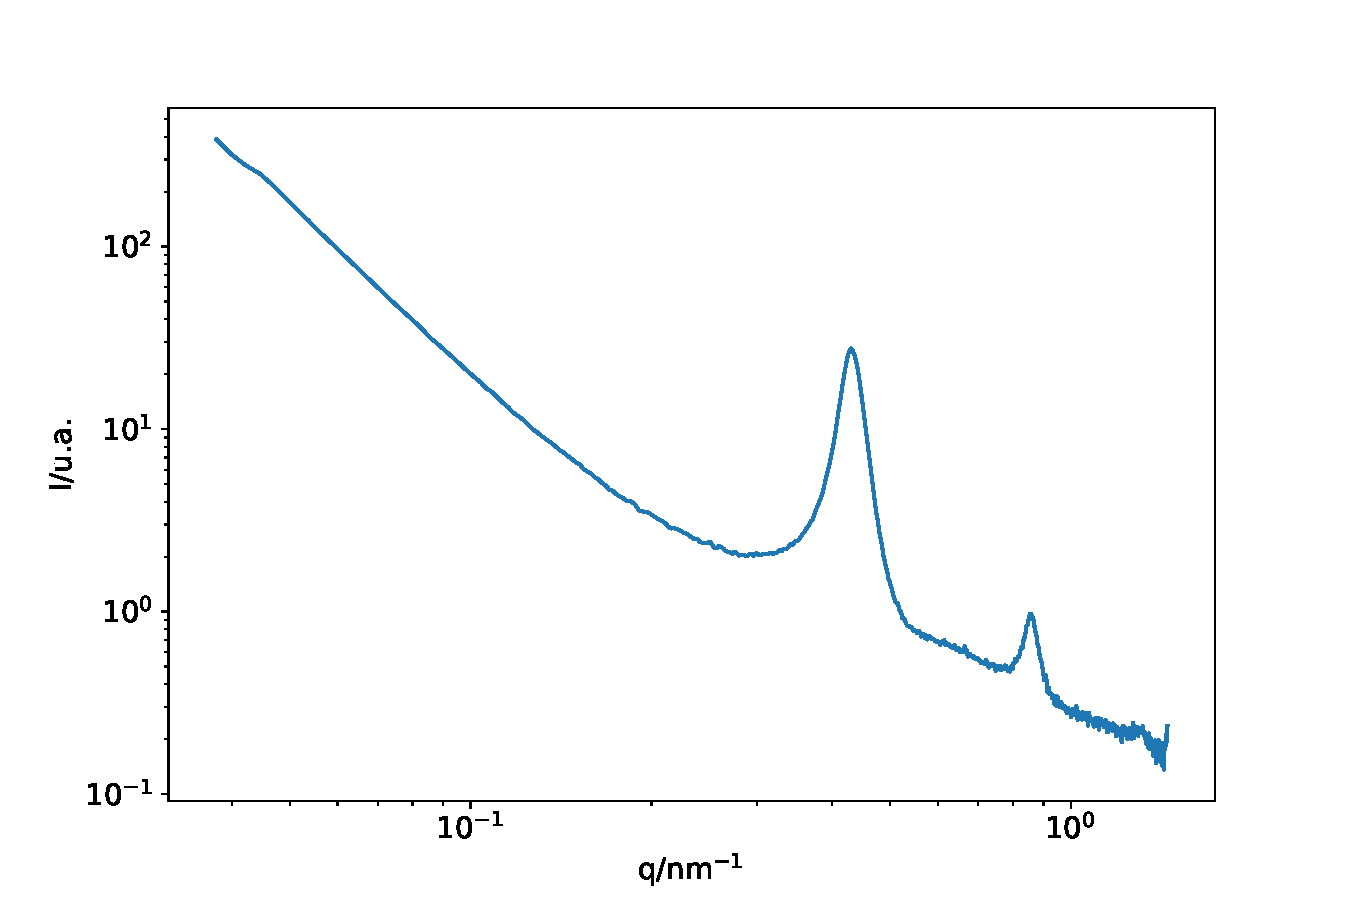
\includegraphics[width=0.7\textwidth]{imagens/saxs/exemplo_SAXS}
			\caption{Curva de espalhamento resultante da integração em \(\phi\) do padrão de espalhamento obtido na fig. \ref{fig:esquema_saxs}. Os picos obtidos nessa figura são resultado da difração de raios-X devido à presença de uma estrutura lamelar em solução.}
			\label{fig:exemplo_saxs}
		\end{figure}
		
		Com o valor de \q{} do primeiro pico, é possível determinar o parâmetro de rede (\emph{lattice parameter}) da mesofase. Para estruturas lamelares, que são de maior relevância para este trabalho, temos que o espaçamento dos picos é de \(1:2:3:4...\). O parâmetro de rede, \(d\), é dado pela Eq. \ref{eqn:SAXS_param_rede_lamela}, e seu significado está ilustrado na figura \ref{fig:saxs_distancia_interlamelar}. É interessante notar a semelhança desse método de identificação com a determinação do raio de esferas pelos mínimos da figura \ref{fig:espalhamento_esfera}. Os picos observados também são chamados de picos de Bragg, mostrando a íntima relação com a área de difração de raios-X, e a modelagem desse tipo de curva de espalhamento utiliza os índices de Miller dos objetos.
	
		\begin{equation}
			q = \dfrac{2\pi}{d}
			\label{eqn:SAXS_param_rede_lamela}
		\end{equation}
		
	
		\begin{figure}[h]
			\centering
			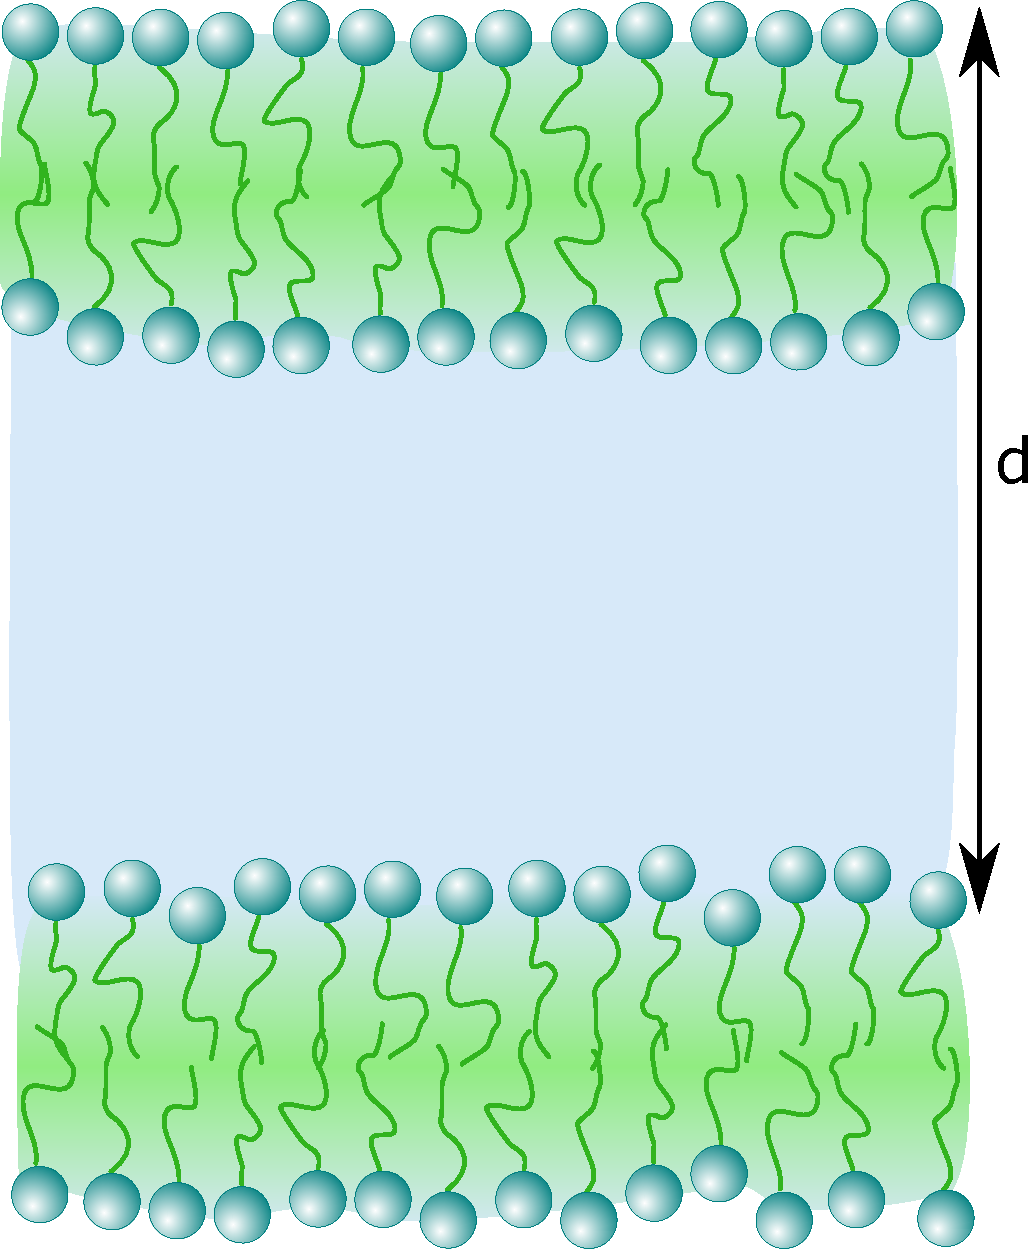
\includegraphics[width=0.35\textwidth]{imagens/saxs/distancia_interlamelar}
			\caption{Distância interlamelar}
			\label{fig:saxs_distancia_interlamelar}
		\end{figure}

		% todo: colocar a referência do artigo do guilherme
		A partir da distância interlamelar, é possível calcular a espessura lamelar (\(d_{\text{HC}}\)) caso a fração volumétrica de surfactante (\(\phi_s\)) e solvente (\(\phi_w\)) também sejam conhecidos. Nesse caso, seria necessário somente relacionar as proporções das regiões com o total, a distância interlamelar. Esse é o princípio do método descrito em X. A fração volumétrica de surfactante pode ser obtida pela Eq. \ref{eqn:SAXS_frac_volum}, cujos parâmetros estão explicados na tabela \ref{tab:ur_fracvol_descr}.
		
		\begin{equation}
			\phi_s = \dfrac{V_{\textit{HC}}\left( \dfrac{w_{s}}{M_{s}} \right)}{\left( V_{\textit{HC}} + V_{P} \right)\dfrac{w_{s}}{M_{s}} + V_{w}\dfrac{w_{w}}{M_{w}}}
			\label{eqn:SAXS_frac_volum}
		\end{equation}
		
	% + V_{\textit{ur}}\dfrac{w_{\textit{ur}}}{M_{\textit{ur}}
	
		\begin{table}[H]
			\IBGEtab{\caption{Descrições das variáveis da equação \ref{eqn:SAXS_frac_volum} \label{tab:ur_fracvol_descr}}}
			{\begin{tabular}{r l}
				\toprule
				           Variável & Descrição                                               \\ \midrule
				              \(s\) & Fração volumétrica de surfactante                       \\
				\(V_{\textit{HC}}\) & Volume molar parcial da cadeia alquílica do surfactante \\
				          \(V_{P}\) & Volume molar parcial da cabeça do surfactante           \\
				          \(w_{s}\) & Fração mássica de surfactante                           \\
				          \(M_{s}\) & Massa molar do surfactante                              \\ \midrule
				          \(V_{w}\) & Volume molar parcial de água                            \\
				          \(w_{w}\) & Fração mássica de água                                  \\
				          \(M_{w}\) & Massa molar da água                                     \\ \bottomrule
			\end{tabular}
			}%
			{}%
		\end{table}

		% todo: colocar como que esses valores podem ser estimados
		
		Sabendo então a fração volumétrica de surfactante, podemos obter a espessura da lamela a partir da distância total pela simples relação da equação \ref{eqn:SAXS_espessura_lamelar}.
		
		\begin{equation} \label{eqn:SAXS_espessura_lamelar}
			d_{\text{HC}} = \phi_s d
		\end{equation}
		
		Em suma, o espalhamento de raios-X em baixos ângulos é uma técnica que permite a obtenção de parâmetros estruturais microscópicos médios do sistema, desde que se conheça qual são as estrutura mais prováveis presentes na amostra. Isso é feito através do ajuste de modelos desenvolvidos pela descrição matemática das estruturas, pelo método dos mínimos quadrados, ou também pela indexação de picos.
		
	\chapter{Fluorescência}
		\section{Diagrama de Jablonski}
		
		O fenômeno de fluorescência é uma subdivisão do fenômeno luminescência, posição que compartilha com a fosforescência. A diferença entre os dois fenômenos está no mecanismo de transição eletrônica, que também altera os tempos de vida dos dois fenômenos. De forma geral, os tempos de vida de fluorescência são da ordem de \(10^{-8} s\), já a fosforescência os tempos de vida variam de milissegundos a segundos. Neste trabalho, somente o fenômeno da fluorescência é de importância.
		
		Uma maneira de se visualizar os fenômenos de luminescência é através do diagrama de Jablonski. Nesse tipo de diagrama, o eixo y representa energia, e as várias linhas representam níveis energéticos. A figura \ref{fig:diagrama_jablonski} mostra um diagrama de Jablonski onde os fenômenos de absorção, fluorescência e fosforescência estão ilustrados. Os níveis \(S\) representam os estados singleto, e seu subíndice representa o nível eletrônico, sendo 0 o fundamental, que é marcado como uma linha mais grossa. Os níveis vibracionais são marcados de 0 a 4 nesse diagrama, com uma linha mais fina. As linhas pontilhadas representam processos não-radiativos e as linhas cheias representam processos radiativos. As cores das linhas são proporcionais aos comprimentos de onda envolvidos, mas não descrevem as cores reais. O nível tripleto é representado como \(T_1\).  % todo: colocar o que é um singleto.
		
		\begin{figure}[h]
			\centering
			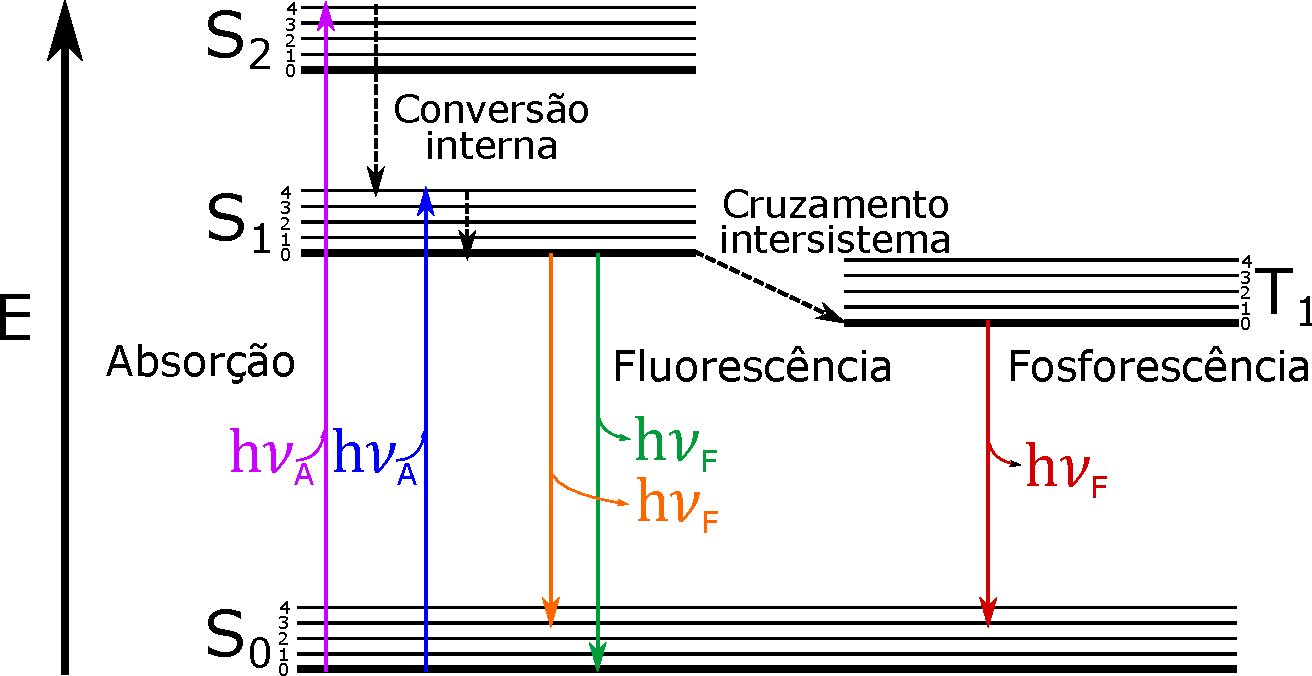
\includegraphics[width=0.7\textwidth]{imagens/fluor/diagrama_jablonski}
			\caption[Diagrama de Jablonski]{Diagrama de Jablonski. As linhas horizontais indicam níveis energéticos, com níveis mais altos para cima. As setas indicam transições radiativas e as setas tracejadas indicam transições não radiativas. As cores das setas são proporcionais à energia de cada transição. Por simplicidade, não estão representados os fenômenos de extinção, transferência de energia e interação com o solvente. Adaptado de X}
			\label{fig:diagrama_jablonski}  % todo: colocar a referência dessa adaptação
		\end{figure}  
		
		\section{Origem do fenômeno de fluorescência}
		
		Quando uma molécula absorve radiação no comprimento de onda adequado, um de seus elétrons passa para um nível eletrônico maior, e geralmente para um nível vibracional maior também. Porém, a temperatura ambiente geralmente não é suficiente para manter esses elétrons em níveis vibracionais altos, então eles relaxam rapidamente (\(10^{-12} s\) ou menos) para o nível vibracional fundamental do nível eletrônico excitado, um processo chamado de conversão interna. Essa conversão pode ocorrer de estados eletrônicos mais elevados também. Como essa escala de tempo é muito menor do que a de fluorescência (\(10^{-8} s\)), os elétrons excitados relaxam completamente sua energia vibracional, atingindo um estado excitado termicamente equilibrado.
		
		Após esse equilíbrio térmico, um elétron pode decair para o nível eletrônico fundamental, tanto para níveis vibracionais elevados ou fundamentais, emitindo um fóton de energia igual à transição. Há uma diferença das energias de absorção e de emissão devido à conversão interna e à tendência de ocorrer transições para níveis vibracionais elevados. Essa diferença de energia resulta num deslocamento no comprimento de onda dos espectros de absorção e emissão, chamado de deslocamento de Stokes.
		
		O fenômeno de conversão interna também implica que o espectro de emissão geralmente é independente do comprimento de onda do fóton incidido, pois o espectro de emissão ocorre sempre do estado vibracional fundamental do estado excitado. Essa regra é conhecida como lei de Kasha.
		
		As transições eletrônicas ocorrem numa faixa de tempo muito rápida, de cerca de \(10^{-15} s\). Esse tempo é muito rápido para que tenha ocorrido mudanças nas posições dos núcleos. Isso é conhecido como o princípio de Frank-Condon. Uma das consequências desse princípio é que a probabilidade de uma transição \(S_1 \to S_0\) é igual à probabilidade de uma transição \(S_0 \to S_1\), o que resulta em espectros de emissão e absorção espelhados. Quando o espelhamento não é observado, é possível que o espectro de absorção possua uma absorção para um segundo estado excitado \(S_2\), onde o elétron relaxa rapidamente. Logo, observa-se o somente as transições espelhadas entre os estados \(S_1\) e \(S_0\).
			
		As transições para os estados excitados ocorrem sem alteração do spin do elétron. Porém, caso o elétron troque de spin, no fenômeno chamado de cruzamento intersistema, o novo estado, um tripleto, não possui uma transição permitida para o estado singleto fundamental. Isso faz com que as escalas de tempo para a transição sejam muito maiores do que a fluorescência, onde a transição é permitida.
		
		\section{Rendimento quântico e tempo de vida}
				
		O rendimento quântico é a eficiência de emissão relativo ao número de fótons absorvidos. Quanto mais próximo de 1 for o rendimento quântico, mais intensa é a fluorescência. O tempo de vida é o tempo em que o fluoróforo permanece em seu estado excitado. Quanto maior for o tempo de vida, mais interações podem ocorrer com moléculas ao redor do fluoróforo, e mais informações podem ser obtidas.
		
		A fluorescência é dependente da polaridade do solvente. Isso ocorre porque, geralmente, o fluoróforo no estado excitado possui um dipolo maior do que no estado fundamental. Isso faz com que as moléculas do solvente ao redor do fluoróforo se rearranjem ao redor dele, diminuindo a energia do sistema, aumentando o deslocamento de Stokes. O rearranjo de uma molécula de solvente ocorre na ordem de 40 ps ou menos, e o rearranjo total ocorre em cerca de \(10^{-10} s\). Dependendo da polaridade do solvente, os efeitos do rearranjo podem ser maiores ou menores, resultando em deslocamentos de Stokes diferentes e espectros de emissão de fluorescência deslocados.
		
		Na área de fluorescência existem dois métodos experimentais, a fluorescência estacionária e a fluorescência resolvida no tempo. Na fluorescência estacionária, a amostra é iluminada e observada constantemente. Como os fenômenos de fluorescência são muito rápidos, efetivamente observa-se uma média dos fenômenos que ocorreram durante a observação. Utilizando equipamentos bastante sofisticados, é possível emitir pulsos de radiação curtos e observar o decaimento da fluorescência com o tempo, em escalas de ns. Isso é conhecido como fluorescência resolvida no tempo. Neste trabalho, foi utilizado somente fluorescência estacionária e, de certo modo, uma combinação das duas técnicas, onde observou-se a variação de fluorescência em escalas de ms a minutos.
		
		% todo: colocar as equações para rendimento quÂntico e tempo de vida?
		
		\section{Extinção}
		
		Há fenômenos que conseguem impedir uma molécula de fluorescer, diminuindo a intensidade de fluorescência medido. Esses fenômenos são chamados de extinção (\emph{quenching}). Há pelo menos três mecanismos possíveis para a extinção:
		
		\begin{enumerate}[noitemsep]
			\item Troca eletrônica
			\item Cruzamento intersistemas, ou o efeito do átomo pesado
			\item Transferência eletrônica fotoinduzida.
		\end{enumerate}
		
		Para a extinção ocorrer, é necessário que haja contato entre a molécula do fluoróforo e do \emph{quencher}. No caso de troca eletrônica, há uma molécula que é pobre eletronicamente, chamada de aceptor e o fluoróforo, o doador. Entrando em contato, o doador transfere seu elétron excitado para o aceptor e recebe de volta um elétron no estado fundamental, concertadamente ou não. Isso equilibra as cargas no sistema, e faz com que o aceptor esteja no estado excitado. O aceptor em seguida pode tanto perder a energia por processos radiativos quanto não-radiativos. % todo: pode mesmo por porcesso radiativo?
		% todo: colocar exemplos aqui
		
		O cruzamento intersistemas, mecanismo que também dá origem à fosforescência, pode ser induzido por átomos pesados, como halogênios, devido ao acoplamento spin-órbita. Em solução aquosa, um elétron no estado \(T_1\) relaxa por processos não radiativos pois o tempo de vida desse tipo de transição é muito alto. O oxigênio é um \emph{quencher} bastante comum e consegue extinguir a maior parte dos fluoróforos, sendo que em alguns casos é necessário removê-lo do meio para permitir a observação de fluorescência. O mecanismo de atuação do oxigênio ainda é debatido, porém o mais provável é que o oxigênio, paramagnético, causa um cruzamento intersistema, e o sistema depois perde energia não radiativamente. Outros estudos mostram que podem existir vários mecanismos em conjunto atuando, como, além do cruzamento, transferência de carga e troca eletrônica. % todo: colocar aqui um artigo que fala do brometo em micelas de CTAB
		
		A transferência eletrônica é resultante da formação de um completo entre um doador e um aceptor eletrônico (o fluoróforo pode ser ambos), formando um complexo do tipo \(D_p^+A_p^-\), que pode voltar ao estado fundamental sem emissão, porém em alguns casos é observada a emissão desse complexo. Após a relaxação, o elétron é retornado ao doador. 
		
		Outro parâmetro que pode influenciar a fluorescência é a viscosidade do meio onde o fluoróforo se encontra. Isso depende da estrutura e do mecanismo de emissão específico de cada fluoróforo. A molécula CCVJ possui um aumento de seu rendimento quântico com o aumento da viscosidade do solvente, em soluções de etileno glicol em glicol. Isso ocorre porque a maior viscosidade atrasa a rotação interna de certos grupos em sua estrutura e dificulta um mecanismo de transferência de carga que extingue a fluorescência, aumentando então o rendimento quântico.
		
		% 	Outra consequência do princípio de Frank-Condon é que o fenômeno de absorção, muito rápido, só fornece informações sobre o estado fundamental médio das moléculas e das moléculas de solvente nas imediações. Porém, como a fluorescência é mais demorada, é possível que ocorram interações com outras moléculas em solução, fornecendo informações sobre o ambiente químico do fluoróforo.
		
		% todo: colocar como se calcula singleto e tripleto.
		
	\chapter{Forças intermoleculares e interagregados}
	
	Na natureza existem quatro forças distintas, porém, para o campo dos coloides, a força eletromagnética é de maior importância. As forças comumente estudadas na química, como as interações dipolares, e dispersivas, possuem uma origem fundamentalmente eletrostática. De forma geral, potenciais de interação de pares \(w\) podem ser escritos de acordo com a equação \ref{eqn:energia_livre_generica}. A força \(F\) é obtida pela derivada dessa equação em função da posição (eqn. \ref{eqn:forca_generica}).
	
	\begin{equation}
		w(r) = -\dfrac{C}{r^n}
		\label{eqn:energia_livre_generica}
	\end{equation}
	
	\begin{equation}
		F(r) = -\dfrac{\mathrm{d}w(r)}{\mathrm{d}r} = -n \dfrac{C}{n+1}
		\label{eqn:forca_generica}
	\end{equation}
	
	\noindent onde \(C\) é uma constante de interação, \(r\) é a distância e \(n\) é um fator de distância.
	
	As interações intermoleculares possuem valores de \(n\) entre 4 e 5. Isso permite que não seja necessário considerar o sistema como um todo para calcular as interações intermoleculares, pois as energia de interação decaem rapidamente, sendo efetivas somente em curtas distâncias. Mie propôs uma forma para o potencial de interação adicionando um componente repulsivo, a equação \ref{eqn:forca_mie}.
	
	\begin{equation}
		w(r) = -\dfrac{A}{r^n} + \dfrac{B}{r^m}
		\label{eqn:forca_mie}
	\end{equation}
	
	\noindent onde \(A\) e \(B\) são as constantes de interação atrativa e repulsiva, respectivamente, e \(n\) e \(m\) são os fatores de distância. O potencial de Lennard Jones ocorre quando \(n = 6\), correspondente às atrações de van der Waals, \(m = 12\). Os valores comuns de \(A\) e \(B\) são \(10^{-77}\) J e \(10^{-134}\) J. % todo: isto é no vácuo?
	
	Quando as interações intermoleculares ocorrem através de um meio, como um solvente, é necessário incluir o efeito das moléculas do solvente nos potenciais de interação. Atrações que seriam previamente atrativas podem se tornar repulsivas num solvente, caso a energia necessária para remover as moléculas de solvente excede a energia de aproximação molecular. Além disso, a presença de moléculas de solvente podem alterar propriedades das moléculas de soluto, como seus momentos de dipolo.
	
	Os valores de energia somente serão úteis se comparados com outros fatores, por exemplo, a energia térmica, que age de modo a equilibrar o sistema e afastar as moléculas. A 1 atm, o valor da energia térmica do solvente é de \(\approx \sfrac{3}{2} kT\), onde \(k\) é a constante de Boltzmann e \(T\) é a temperatura, então interações com energias menores que \(\sfrac{3}{2}kT\) não conseguem so sobrepor ao movimento térmico das moléculas. % todo: ler essa parte e ver se é kT ou 3/2 kT.
	
	As interações intermoleculares possuem três origens distintas:
	
	\begin{enumerate}[noitemsep]
		\item Origem puramente eletrostáticas, como no caso de interações entre íons, dipolos (e quadropolos, etc) permanentes, e interações de polarização.
		\item Origem puramente entrópica, que surgem do comportamento coletivo das moléculas, como as forças osmóticas.
		\item Origem mecânico quântica, como as ligações covalentes, forças de dispersão de van der Waals, ácido-base, forças estérica repulsivas devido ao princípio de exclusão de Pauli.
	\end{enumerate}
	
	\section{Interações Coulombicas}
	
	As interação Coulombica depende do campo elétrico entre uma partícula carregada e a carga de outra partícula próxima. O campo elétrico é dado pela equação \ref{eqn:campo_eletrico}.
	
	\begin{equation}
		E = \dfrac{Q_1}{4\pi\varepsilon_0\varepsilon r^2}
		\label{eqn:campo_eletrico}
	\end{equation}

	\noindent onde \(Q_1\) é a carga da partícula, \(\varepsilon_0\) é a constante dielétrica do vácuo e \(\varepsilon\) é a constante dielétrica relativa do meio em questão. Como pode ser visto, a presença de um meio diminui a força da interação eletrostática por \(\varepsilon\), então em solventes com constantes dielétricas altas, a força eletrostática é bastante enfraquecida. É necessário enfatizar que os termos \(\varepsilon\) e \(\varepsilon_0\) são dependentes da frequência \(\nu\) do campo elétrico aplicado (por exemplo, o campo elétrico oscilatório da luz). Em frequência zero, em condições estáticas, esses termos recebem o nome de constante dielétrica, mas fora dessas condições recebem o nome de permissividade elétrica.
	
	O potencial de interação entre cargas é obtido pelo processo oposto da equação \ref{eqn:forca_generica}, ou seja, pela integração da força eletrostática, dada por \(F = Q_2 E\) (eqn. \ref{eqn:potencial_eletrostático}), utilizando o estado de referência das cargas como sendo no infinito.
	
	\begin{equation}
		w(r) = \int_\infty^r -F(r)dr = \dfrac{z_1z_2e^2}{4\pi\varepsilon_0\varepsilon r}
		\label{eqn:potencial_eletrostático}
	\end{equation}
	
	Interessantemente, a força gravitacional e a interação Coulombica são comparáveis pois possuem um potencial da forma \(1/r\), portanto são de longo alcance, e também são aditivas, isso é, a interação entre dois corpos não é dependente da presença de outras moléculas ao redor. Esse conceito é importante, pois as interações de van der Waals, de grande relevância para coloides, não são aditivas. % todo: ver se é v.d.W. ou se é dispersiva só.
	
	\section{Interações dipolares}
	
	A maioria das moléculas não possui uma carga, mas sim um momento de dipolo, resultante da posição de cargas totais ou parciais em diferentes pontos da molécula. O momento de dipolo é definido como:
	
	\begin{equation}
		u = ql
		\label{eqn:momento_dipolo}
	\end{equation}
	
	\noindent onde \(u\) é o momento de dipolo e \(l\) é a separação entre as cargas \(+q\) e \(-q\). Essas cargas não precisam estar alinhadas, sendo necessário então corrigir esse não alinhamento pela soma vetorial dos momentos de dipolo individuais.
	
	A energia de interação entre duas moléculas dipolares (sendo uma delas fixa) é dada pela equação \ref{eqn:energia_dipolo_dipolo}.
	
	\begin{equation}
		w \left( r , \theta _ { 1 } , \theta _ { 2 } , \phi \right) = - \frac { u _ { 1 } u _ { 2 } } { 4 \pi \varepsilon \varepsilon _ { 0 } r ^ { 3 } } \left[ 2 \cos \theta _ { 1 } \cos \theta _ { 2 } - \sin \theta _ { 1 } \sin \theta _ { 2 } \cos \phi \right]
		\label{eqn:energia_dipolo_dipolo}
	\end{equation}
	
	\noindent onde \(\theta_{ 1 }\) e \(\theta_{ 2 }\) são os ângulos das duas moléculas dipolares em relação à reta que as liga, \(\phi\) é o ângulo de rotação perpendicular a \(\theta_{ 2 }\) de uma das moléculas. É interessante ver que essa interação também é dependente da constante dielétrica, além de ser dependente de \(r^3\).  % todo: pensar se eu devo deixar essa equação ou só colocar a de Keesom
	
	Se os dois dipolos puderem rodar livremente, a energia média dessa interação, conhecida como energia de Keesom é dada por:
	
	\begin{equation}
		w(r) = - \dfrac{u _ { 1 } ^ { 2 } u _ { 2 } ^ { 2 } }{ 3 \left( 4 \pi \varepsilon \varepsilon _ { 0 } \right) ^ { 2 } k T r ^ { 6 } }
		\label{eqn:energia_Keesom}
	\end{equation}
	
	Note que aqui, a dependência com a distância é da ordem de \(r^{-6}\). Essa é uma das componentes das interações de van der Waals.
	
	\section{Interações de polarização}
	
	Átomos ou moléculas submetidos a um campo elétrico se alinham no sentido contrário ao campo. A magnitude desse alinhamento é dependente da polarizabilidade das moléculas, \(\alpha\), e da intensidade do campo, \(E\)  (eq. \ref{eqn:dipolo_induzido}).
	
	\begin{equation}
		u_{ind} = \alpha E
		\label{eqn:dipolo_induzido}
	\end{equation}
	
	A polarizabilidade do material é composta por uma componente devido ao dipolo inerente da molécula, se houver, e outra componente sempre presente, que aparece devido à distorção da nuvem eletrônica dos átomos ou moléculas, chamada de polarizabilidade eletrônica, \(\alpha_0\).
	
	A equação de Debye-Langevin relaciona a polarizabilidade total com a polarizabilidade eletrônica e o momento de dipolo (eq. \ref{eqn:debye_langevin}).
	
	\begin{equation}
		\alpha = \alpha _ { 0 } + \dfrac{u ^ { 2 }}{ 3 k T }
		\label{eqn:debye_langevin}
	\end{equation}
	
	Uma maneira de se visualizar essa polarização é considerando um átomo de hidrogênio de Bohr. Quando esse átomo é colocado em um campo elétrico, a posição relativa do elétron e do próton configura um dipolo, que irá interagir com o campo, apesar de que o átomo não possui um momento de dipolo permanente.
	
	Uma consequência da polarização das moléculas é justamente a constante dielétrica, que é medida colocando-se o material entre duas placas carregadas de um capacitor. Devido ao campo elétrico, as moléculas alinham seus dipolos, naturais e induzidos, contrariamente ao campo. A soma desses dipolos alinhados gera um campo contrário ao campo aplicado \(E_0\), diminuindo o campo efetivo \(E\). A razão \(\sfrac{E_0}{E}\) resulta na constante dielétrica do meio. Quanto maior for a polarização, maior é a queda do campo efetivo, e maior é a constante dielétrica. Há solventes que possuem mecanismos adicionais para gerar polarização, como o deslocamento de cargas por distâncias significativamente maiores que os tamanhos moleculares. Um exemplo disso é a água, onde elétrons ou prótons sendo transportados pelas ligações de hidrogênio, e amidas secundárias, cujos valores de constante dielétrica podem chegar até 180.

	Outra consequência da polarização de moléculas é o surgimento de uma força entre os dipolos permanentes e dipolos induzidos, chamada de interação de Debye, cujo potencial de energia é dado pela equação \ref{eqn:energia_Debye}.
	
	\begin{equation}
		w ( r ) = - \frac { \left[ u _ { 1 } ^ { 2 } \alpha _ { 02 } + u _ { 2 } ^ { 2 } \alpha _ { 01 } \right] } { \left( 4 \pi \varepsilon _ { 0 } \varepsilon \right) ^ { 2 } r ^ { 6 } }
		\label{eqn:energia_Debye}
	\end{equation}
	
	\noindent onde os subíndices \emph{1, 2} indicam as propriedades (momentos de dipolo \(u\) e polarizabilidades eletrônicas \(\alpha_0\)) de duas moléculas/átomos diferentes. Da mesma maneira que a energia de Keesom (eq. \ref{eqn:energia_Keesom}), a dependência da energia de Debye é proporcional a \(r^{-6}\).
	
	Quando moléculas estão em um meio composto por outras moléculas também com polarizabilidade eletrônica definida, as polarizabilidades de excesso se tornam relevantes, ou seja, é a diferença entre a polarizabilidade de uma molécula com a polarizabilidade natural do meio. Essa abordagem assume que as propriedades são contínuas, o que apresenta suas limitações quando as distâncias de interação são bastante curtas. A equação \ref{eqn:polarizabilidade_excesso} mostra como a polarizabilidade de uma molécula esférica \(i\), com constante dielétrica \(\varepsilon_i\) e volume \(v_i\), é afetada ao estar num meio de constante dielétrica \(\varepsilon\).
	
	\begin{equation}
		\alpha_i = 3 \varepsilon_{ 0 } \varepsilon \left( \dfrac{\varepsilon_i - \varepsilon}{\varepsilon_i + 2 \varepsilon}  \right) v_i
		\label{eqn:polarizabilidade_excesso}
	\end{equation}
	 
	 Essa equação pode ser utilizada para descobrir a polarizabilidade total de uma molécula no estado gasoso (onde \(\varepsilon = 1\)), relação conhecida como a equação de Clausius-Mossotti (eq. \ref{eqn:clausius_mossotti}).
	 
	 \begin{equation}
		\dfrac { \alpha } { \left( 4 \pi \varepsilon _ { 0 } \right) } = \left( \dfrac { \varepsilon - 1 } { \varepsilon + 2 } \right) \dfrac { 3 v } { 4 \pi }
		\label{eqn:clausius_mossotti}
	 \end{equation}
	
	A polarizabilidade eletrônica \(\alpha_0\) pode ser calculada por uma modificação da equação de Clausius-Mossotti. Ao invés de se utilizar as constantes dielétricas, onde a frequência de perturbação é zero, é necessário utilizar as permissividades na frequência do UV-visível. Na região do UV-visível, a equação \ref{eqn:permissividade_e_indice_refrac} relaciona o índice de refração, definido na equação \ref{eqn:def_n}, com a permissividade elétrica.
	
	\begin{equation}
		\varepsilon(\nu) = n(\nu)^2
		\label{eqn:permissividade_e_indice_refrac}
	\end{equation}
	
	\begin{equation}
		n = \dfrac{c_0}{c}
		\label{eqn:def_n}
	\end{equation}
	
	\noindent onde \(n\) é o índice de refração, \(c_0\) é a velocidade da luz no vácuo e \(c\) é a velocidade da luz no meio.
	
	Com isso, pode-se obter a equação de Lorenz-Lorentz, eq. \ref{eqn:lorenz_lorentz}, que relaciona a polarizabilidade eletrônica com o índice de refração. Em frequências altas, acima de \(10^{12}\) Hz, dipolos moleculares não possuem tempo suficiente para responder a um campo, então a polarização é devido somente à polarização eletrônica. Essa separação de comportamentos a frequência zero e frequência no UV-Vis, utilizando a constante dielétrica e o índice de refração ocorrerá em outras equações desta seção.
	
	\begin{equation}
		\dfrac { \alpha _ { 0 } } { \left( 4 \pi \varepsilon _ { 0 } \right) } = \left( \dfrac { n ^ { 2 } - 1 } { n ^ { 2 } + 2 } \right) \dfrac { 3 v } { 4 \pi }
		\label{eqn:lorenz_lorentz}
	\end{equation}
	% todo: falar sobre a interação dipolar por volume
	\section{Interações dispersivas}
	
	As forças de van der Waals são compostas pelas forças dispersivas, junto com as forças de Keesom e Debye. Esse nome vem da dispersão da luz na região do visível e ultravioleta. As forças dispersivas são as mais importantes das três forças, pois estão presentes em todas as moléculas e átomos, podem ser de longa distância, atrativas ou repulsivas, e não são aditivas.
	
	A origem das forças dispersivas está na eletrodinâmica quântica, porém sua natureza ainda é essencialmente eletrostática. Um átomo ou molécula não polar possui momento de dipolo temporal médio igual a zero, mas, como mencionado para o átomo de hidrogênio de Bohr, a cada momento existe um momento de dipolo devido à disposição da nuvem eletrônica ao redor do núcleo. Esse momento de dipolo instantâneo irá induzir um momento de dipolo num átomo vizinho, e estes irão interagir eletrostaticamente. A média temporal dessa atração é não nula, apesar da média temporal dos momentos de dipolo ser nula. O momento de dipolo instantâneo do átomo de hidrogênio de Bohr é de 2,5 Debye, o que não é pequeno.
	
	A energia de interação de van der Waals entre dois átomos, 1 e 2,  no vácuo pode ser descrita pela equação \ref{eqn:energia_dispersiva}, proposta por London em 1937.
	
	\begin{equation}
		w(r) = - \frac { 3 } { 2 } \frac { \alpha _ { 01 } \alpha _ { 02 } } { \left( 4 \pi \varepsilon _ { 0 } \right) ^ { 2 } r ^ { 6 } } \frac { h \nu _ { 1 } \nu _ { 2 } } { \left( \nu _ { 1 } + \nu _ { 2 } \right) }
		\label{eqn:energia_dispersiva}
	\end{equation}
	
	\noindent onde \(h\) é a constante de Planck e \(\nu\) é a frequência de absorção do átomo. O termo \(h\nu_i\) pode ser substituído por \(I_i\), a energia de ionização do átomo \(i\). É possível notar a dependência de \(r^{-6}\) que as outras energias também possuem.
	
	% todo: mencionar a energia dispersiva por volume, e como ela é constante
	
	Com a terceira equação, é possível obter o panorama completo da energia de interação de van der Waals obtido pela soma das três energias (equação \ref{eqn:vdw}.
	
	\begin{subequations}
	\begin{align}
		w_{\mathrm{VDW}}(r) &= -C_{\mathrm{VDW}}/r^{6} = -\left[C_{\mathrm{Debye}}+C_{\mathrm{Keesom}}+C_{\mathrm{London}}\right]/r^{6} \label{eqn:vdw_geral} \\
							&= - \left[ \left( u_{1}^{2}\alpha_{02} + u_{2}^{2}\alpha_{01} \right)   + \frac{u_{1}^{2}u_{2}^{2}}{3kT} + \frac{3\alpha_{01}\alpha_{02}h\nu_{1}\nu_{2}}{2\left(\nu_{1} + \nu_{2}\right)}\right]/\left(4\pi\varepsilon_{0}\right)^{2}r^{6} \label{eqn:vdw_completa}
	\end{align}
	\label{eqn:vdw}
	\end{subequations}
	
	Porém, essa equação possui algumas limitações. Não são consideradas absorções além da primeira, e não é possível levar em consideração o meio. MacLachlan utilizou uma somatória de todas as absorções para expandir a abrangência da equação, e utilizou propriedades de excesso para poder considerar a presença de um meio. Assumindo que todos os meios possuem a mesma energia de absorção, e que as partículas \emph{1} e \emph{2} sejam iguais e dispersas no meio \emph{3}, é possível obter a equação \ref{eqn:energia_maclachlan}, onde as contribuições estáticas, onde \(\nu = 0\) (Debye e Keesom) foram separadas das contribuições de frequências altas, onde predominam as interações dispersivas.
	
	\begin{equation}
		w ( r ) = w ( r ) _ { \nu = 0 } + w ( r ) _ { \nu > 0 } \approx - \left[ 3 k T \left( \frac { \varepsilon _ { 1 } ( 0 ) - \varepsilon _ { 3 } ( 0 ) } { \varepsilon _ { 1 } ( 0 ) + 2 \varepsilon _ { 3 } ( 0 ) } \right) ^ { 2 } + \frac { \sqrt { 3 } h \nu _ { e } } { 4 } \frac { \left( n _ { 1 } ^ { 2 } - n _ { 3 } ^ { 2 } \right) ^ { 2 } } { \left( n _ { 1 } ^ { 2 } + 2 n _ { 3 } ^ { 2 } \right) ^ { 3 / 2 } } \right] \frac { a _ { 1 } ^ { 6 } } { r ^ { 6 } }
		\label{eqn:energia_maclachlan}
	\end{equation}
	
	\noindent onde \(a_1\) é o raio da molécula 1.
	
	% Polarizabilidade de excesso
	% \alpha _ { 1 } ( \nu ) = 4 \pi \varepsilon _ { 0 } \varepsilon _ { 3 } ( \nu ) \left( \frac { \varepsilon _ { 1 } ( \nu ) - \varepsilon _ { 3 } ( \nu ) } { \varepsilon _ { 1 } ( \nu ) + 2 \varepsilon _ { 3 } ( \nu ) } \right) a _ { 1 } ^ { 3 }
	
	% todo: falar sobre a constante de Hamaker e outras coisas importantes para a discussão
		\section{Atração coloidal}
		% Falar sobre como as atrações de vdW em coloides são aditivas, e sobre o problema enfrentado.
		% Falar sobre os estudos do físico para tentar contornar esse problema.
		% Falar sobre DLVO
		\section{Constante de Hamaker}
		% Colocar a equação e falar como que se obtêm os valores
	\chapter{Micelas gigantes}
		\label{chap:micelas_gigantes}
		\section{Crescimento de micelas}
		% Falar sobre o diagrama de fases de micelas
		% Procurar um pouco, na tese da Danila e em teses anteriores do grupo, sobre o que falar a mais de micelas
		% todo: completar esta seção
		As micelas crescem.
		% Falar sobre os tempos de relaxação vistos por Hoffmann por birrefringência elétrica
		\section{Termodinâmica de micelas}
		% Falar sobre a energia das pontas. Pesquisar sobre o que falar.
		% Fazer uma breve introdução sobre ITC e o que se observa.
		% Falar sobre o ITC e como ele consegue enxergar os processos de micelização
		% todo: fazer esta parte
		As micelas tem pontas com energia superior.
		\section{Comportamento reológico}
		% Falar sobre como identificar visualmente micelas gigantes, como o recoil
		% Falar sobre as várias estruturas que elas possuem, e como a concentração de salicilato afeta as estruturas
		% Falar sobre as G', G'' e o modelo de Maxwell.
		% Falar sobre o tempo de relaxação micelar.
		% Falar sobre os sticky contacts que o Hoffmann tanto gosta.
		% Falar do diagrama de viscosidade no repouso (RH).
		\section{Comportamento calorimétrico}
		
		%		Para micelas gigantes, fixa-se uma concentração de aditivo e depois surfactante é titulado. O padrão da curva de $\Delta H \times C_{\textrm{surf}}$ é bastante característico. No início há muito NaSal e pouco TTAB, e ocorre a formação de micelas esféricas com NaSal. À medida que mais NaSal é incorporado, são formadas micelas mistas cilíndricas curtas . Numa determinada concentração, ocorre uma queda bastante brusca no valor de $\Delta H$, devido à fusão de várias micelas cilíndricas, formando micelas gigantes. A diferença de entalpia entre os estados final e inicial dessa queda brusca caracteriza $\Delta H_{\textrm{WLM}}$. A concentração no ponto mínimo caracteriza $c_{\textrm{WLM}}$%\cite{Ito2016}.
		%		
		%		Com a técnica de ITC, pode-se observar o quão favorável é a formação de micelas gigantes em determinadas condições. Quanto menor for $c_{\textrm{WLM}}$, mais favorável é a formação das micelas. A $c_{\textrm{WLM}}$ é referente ao grau de incorporação de aditivo na etapa de formação de micelas%\cite{Ito2016}
		\section{Espalhamento de luz}
		\section{Efeito do solvente}
		\label{sec:efeito_solvente}
		% Falar mais profundamente sobre os estudos do Hoffmann
		% Falar sobre a hidrofilicidade da superfície micelar, o t3 de relaxação e a relação com os perfis de viscosidade.
		
		
%	\chapter{Análise Multivariada}
%		\section{Técnicas de classificação}
%			\subsection{Normalização dos dados}
%			\subsection{PCA}
%			\subsection{HCA}
%		\section{Técnicas de regressão}
%			\subsection{Regressão Multivariada}
%			\subsection{PCR}
%			\subsection{PLS}
\part{Materiais e Métodos}
	\chapter{Reagentes}
	
	Os reagentes utilizados, suas respectivas purezas e os fabricantes se encontram na tabela \ref{tab:reagentes}.
	
	\begin{table}[h]
		\IBGEtab%
		{\caption{Reagentes, pureza e fabricantes}
		\label{tab:reagentes}}%
	    {
		\centering
		\begin{tabular}{c c p{3.2cm}}
			\toprule
			Reagente  & Pureza                                          & Fabricante                                                  \\ \midrule
			  CTAB    & \(\geqslant 98\%\)                              & Sigma Aldrich                                               \\
			  TTAB    & \(\geqslant 99\%\)                              & Sigma Aldrich                                               \\
			  DTAB    & \(\geqslant 98\%\)                              & Sigma Aldrich                                               \\
			  NaSal   & \(99{,}5\%\)                                    & Sigma Aldrich                                               \\
			Glicerina & \(85\%\) / \agua & Merck                                                       \\
			Sacarose  & \(\geqslant 99{,}5\%\)                          & Sigma Aldrich                                               \\
			  Ureia   & \(\geqslant 99{,}5\%\)                          & Sigma Aldrich                                               \\
			  DMSO    & \(\geqslant 99{,}5\%\)                          & Sigma Aldrich                                               \\
			  1,3BD   & \(99{,}5\%\)                                    & Sigma Aldrich                                               \\
			  Água    & \(\sigma = 18{,}2M\Omega\).cm                   & Millipore Direct-Q\textregistered{} \newline 3 UV com bomba \\ \bottomrule
		\end{tabular}}%
		{}
	\end{table}
	
	% Todo: colocar a estrutura das moléculas aqui
	
             %		Sucralose                       &                                                 &                                                             \\
	% todo: ver se coloco algo da sucralose aqui
	
	\chapter{Reologia}
		\section{Preparo das amostras}
		\label{sec:reologia_preparo_amostra}
		O preparo de amostras de reologia deve ser feita de modo a garantir a completa homogeneização, e perda de memória reológica da amostra. A densidade do solvente é utilizada para os cálculos de concentração, para se determinar as concentrações, em \mM, do surfactante e de NaSal. Não foi considerada a alteração de densidade pela adição de surfactante e NaSal, somente dos aditivos.
		
		Após a pesagem dos componentes em balanças de precisão, frequentemente partindo de soluções estoque altamente concentradas, as amostras são aquecidas até 50°C em banho maria e homogeneizadas por meio de agitação manual e com vórtex. Temperaturas elevadas auxiliam na dissolução dos componentes e diminuem a viscosidade do meio, por também desfavorecerem o crescimento das micelas. Após já homogeneizadas, as amostras são mantidas a 50°C, e depois são resfriadas lentamente até temperatura ambiente removendo-se o aquecimento do banho maria. Neste instante, as amostras estão prontas para análise reológica. As amostras eram preparadas no mínimo com 24h de antecedência.
		
		\section{Análises reológicas} \index{reologia!preparo de amostra}

		% todo: checar se só foi utilizado esse reômetro
		Todas as análises reológicas foram realizadas utilizando a geometria placa-placa de 35 mm de diâmetro (P35 Ti L) no reômetro Haake Mars III da Thermo Scientific. Antes de cada análise, a inércia do porta-rotor (\emph{spindle}) e do rotor eram determinadas de modo a controlar por erros relacionados ao encaixe manual do rotor. Também era determinado o ponto zero de altura, onde há o contato do rotor com a base, de modo a estabelecer um espaçamento de 1,000 mm durante as análises. A temperatura era controlada pela combinação de um banho termostatizado e de aquecimento na base, e monitorada por meio de sensores na base.
		
		As amostras são transferidas para a placa do reômetro simplesmente vertendo-se os tubos falcon até que a área de análise estivesse coberta. Caso as amostras fossem resistentes demais, uma espátula era utilizada para cortar e espalhar o gel sobre a base. Em seguida, o rotor era abaixado e observava-se se não havia falta de amostra em algum ponto. Caso houvesse falta, a amostra era recuperada e reaplicada na base. O cisalhamento causado pela transferência de amostra e pelo abaixamento do rotor não foram levados em consideração nas análises. A amostra era coberta por um protetor de teflon de modo a minimizar a perda de solvente durante a análise.
		
		Os métodos de análise são montados de acordo com as necessidades de cada amostra. Em comum, somente há a etapa de termostatização por 5 minutos na temperatura de análise. As etapas possíveis são:
		
		\begin{itemize} 
			\item Análise de varredura de tensão. A faixa de valores de tensão estudados foram geralmente de 0,01 Pa até 5 Pa, espaçados logaritmicamente, analisados a 1 Hz. Com essa análise é possível determinar a região linear, onde os valores de G' e G'' estão constantes, independente da tensão aplicada. Caso uma tensão alta demais seja aplicada, começa a ocorrer a desestruturação do material, e os valores de G' e G'' diminuem.
			
			\item Análise de varredura de frequência, numa tensão dentro da região linear, geralmente 1 Pa. A faixa de frequência estudada varia de acordo com as necessidades da amostra e com o tempo disponível, pois quanto menor a frequência estudada, maior é o tempo de análise. A faixa de frequência habitual é de 0,01 Hz a 10 Hz (ou 0,0628 rad.s\menosUm{} a 62,83 rad.s\menosUm), e 6 medidas por década, espaçadas logaritmicamente. Este tipo de experimento demora cerca de 20 minutos. O modo utilizado em todas as análises foi CS (Control Shear).
			
			\item Análise de curva de fluxo. As taxas de cisalhamento (\(\dot{\gamma}\)) utilizadas geralmente variavam de 0,001 s\menosUm{} a 10 s\menosUm. Caso o platô Newtoniano não fosse observado, diminuia-se a taxa aplicada. Obtinha-se entre 10 e 20 pontos espaçados logaritmicamente. As medidas eram obtidas no modo CR (Control Rate).
		\end{itemize} \index{reologia!sequência experimental}
		
		Ao montar-se um plano experimental, pode-se configurar o equipamento para exportar os dados obtidos de acordo com uma configuração tabular específica, para um arquivo de texto. Isso facilita posteriormente o tratamento de dados. Além disso, o nome do arquivo pode ser gerado automaticamente pela composição da amostra, a hora e a data de análise.
		
		\section{Tratamento de dados de reologia oscilatória}
		
		Para micelas gigantes, a obtenção de informações microscópicas da amostra geralmente é realizada através de um ajuste das curvas de G' e G'' ao modelo de Maxwell. Com esse ajuste, é possível obter informações como o tempo de relaxação estrutural das micelas e os módulos elásticos das soluções. Para realizar o tratamento, os dados foram importados ou para o software Origin\textcopyright{} 9 ou Python, e o modelo de Maxwell foi ajustado para G' e G'' utilizando-se um conjunto de parâmetros para ambas as curvas, obtidos pelo método dos mínimos quadrados.
		
		A região utilizada para os ajustes depende da qualidade subjetiva dos pontos. Por exemplo, em altas frequências de oscilação, a confiabilidade dos valores de G' e G'' é menor devido à inércia do rotor. Por essa razão, há muito ruído em altas frequências, e a região de ruído varia de amostra para amostra. Dessa maneira, cada dado é analisado separadamente, removendo-se os pontos ruidosos.
		% todo: colocar referência das seções relevantes.
		% todo: quando eu analisar novamente os dados de reologia oscilatória das amostras com aditivos, onde eu farei também análises de Cole Cole e descobrirei outros tempos de relaxação, colocar aqui como que esses métodos foram feitos
		
		\section{Tratamento de dados de curvas de fluxo} \index{reologia!curva de fluxo}
		
		Micelas gigantes são fluídos conhecidamente pseudoplásticos, ou seja, sua viscosidade aparente (\(\eta\)) diminui com o aumento da taxa de cisalhamento (\(\dot{\gamma}\)). Em baixos valores de \(\dot{\gamma}\), a viscosidade aparente é constante, e esse valor é chamado de viscosidade no repouso, \(\eta_0\). Esse valor é de maior interesse para este trabalho. Para obter esse valor, é possível realizar ajustes lineares da região onde a viscosidade é constante, forçando-se a inclinação da reta a zero. Em suma, isso obtém o valor médio da viscosidade no repouso. Há também modelos matemáticos que podem ser usados, como Carreau e Cross, e a viscosidade no repouso, dentre outros parâmetros, podem ser obtidos pelo método dos mínimos quadrados.
		
		Dados de curva de fluxo também são passíveis de desvios, que dificultam os ajustes. Nas amostras observadas aqui, geralmente há problemas em baixas taxas de cisalhamento. Para contornar esse problema, é necessário selecionar uma faixa de valores para o ajuste, o que pode ser feito manualmente e programaticamente. O apêndice \ref{sec:apn_tratamento_CF} mostra brevemente como o programa para tratamento de curva de fluxo funciona, os problemas frequentes encontrados com curvas de fluxo e como contorná-los.
		
	\chapter{Calorimetria de titulação isotérmica} 
		\section{Preparo de amostra e uso do equipamento} \index{ITC!experimental}
		\label{sec:preparo_amostra_itc}
		% todo: verificar qual é a variação de volume
		
		Na calorimetria de titulação isotérmica (ITC), titula-se uma solução contida numa seringa em outra solução contida numa cela. Esse processo pode liberar ou absorver calor, e a quantidade de calor absorvido ou liberado é dependente de todos os processos que ocorrem durante a injeção, por exemplo, diluição e micelização. Essa sensibilidade exige que muito cuidado seja tomado na preparação de amostra, de modo a obter soluções bastante limpas e homogêneas, sem interferentes, e com concentração bem conhecida. Além disso, o solvente de ambas as soluções (da seringa e cela) devem ser estritamente os mesmos, para impedir que exista um sinal de mistura do solvente.
		
		Quando o solvente das amostras é diferente de água, prepara-se inicialmente a quantidade necessária de solvente para todas as amostras, e esse solvente é utilizado tanto para as soluções da cela quanto da seringa. Após isso, os componentes sólidos são adicionados às soluções, que são homogeneizadas e depois ficam em repouso por no mínimo 24 horas. Variações de densidade são somente consideradas na formação do solvente binário, e não são consideradas nas outras etapas pois a concentração das espécies é menor. As soluções foram preparadas em tubos falcon previamente limpos com etanol, água de torneira e água deionizada três vezes.
		
		A escolha das concentrações das espécies na cela e na seringa dependem do sistema que será estudado, e da região do entalpograma que se deseja observar. Neste trabalho, o sistema de referência é uma solução 1,5 \mM{} de NaSal na cela e TTAB 14 \mM{} na seringa, com água deionizada como o solvente em comum. Esse sistema permite a observação do início dos entalpogramas, antes da micelização, a formação de micelas gigantes e o início da região de transformação para micelas esféricas. Caso se deseja observar o perfil completo, é necessário aumentar a concentração de TTAB, porém perde-se resolução e o início do entalpograma. Caso o solvente seja alterado, é necessário realizar medidas prévias para determinar a melhor concentração de surfactante para a região que se deseja observar.
		
		% todo: achar certinho os volumes e colocar aqui.
		Neste trabalho, utilizou-se tanto o VP-ITC da Microcal quanto o PEAQ-ITC da Malvern. A diferença entre esses sistemas é, essencialmente, o volume da seringa e da cela, que é menor no PEAQ-ITC. A limpeza deve ser feita antes de qualquer análise.
		
		Para a limpeza do VP-ITC, lava-se a seringa internamente com aproximadamente 15 mL de etanol, seguido de 25 mL de água deionizada. A cela é limpa preenchendo-se a cela 5 vezes com etanol, e em seguida 500 mL de água deionizada recém preparada é passada continuamente pela cela por meio de um sistema de vácuo. Após isso, remove-se o restante de água na cela, e coloca-se a solução na cela, tomando cuidado para remover bolhas e o excesso de solução. A seringa é seca, passando-se ar por seu interior, e depois é preenchida com sua solução e o conteúdo é purgado e repreenchido duas vezes. Caso seja necessário, é possível colocar Contrad 70 20\% na cela e aumentar a temperatura até 50°C por algumas horas para remover alguma sujeira resistente, como proteínas.
		
		% todo: checar se o Soak é a 50°C.
		A limpeza do PEAQ-ITC é feita automaticamente pelo equipamento, com três modos disponíveis. Para medidas de rotina, utiliza-se somente a função \emph{Rinse}. Nesse modo, passa-se somente água na cela e na seringa, água é inicialmente passada, seguido de metanol, para auxiliar na secagem. Caso o sistema precise de uma limpeza mais profunda, por exemplo, se polímero ou proteína foi utilizado num experimento anterior, utilizou-se o método \emph{Wash}, que usa Contrad 70 20\% para limpar a cela. Em casos extremos, utilizou-se a função \emph{Soak}, onde uma solução de Contrad 70 20\% é colocada na cela por 1h a 50°C. A cela e a seringa são preenchidas da mesma maneira que no VP-ITC.
		
		Os parâmetros de análise são: % todo: pensar melhor nessa frase
		% todo: pesquisar em trabalhos meus anteriores para ver o que eu coloco
		
		\begin{itemize}[noitemsep]
			
			\item Concentração: A concentração das espécies na seringa e na cela devem ser conhecidas com precisão, e podem ser alteradas após o experimento.
			
			\item Sensibilidade: Quanto maior a sensibilidade, menor é o valor absoluto que calor que é observado, porém mais detalhes conseguem ser observados. Neste trabalho, a sensibilidade escolhida variou bastante, de acordo com a amostra.
			
			\item \emph{Reference Power}: Esse valor indica a quantidade de calor que é fornecida continuamente para a cela de referência e de amostra. A faixa de valores disponíveis é dependente da sensibilidade escolhida. Cada sensibilidade possui um valor máximo e um valor mínimo de calor que pode ser fornecido à cela. Por esse motivo, a escolha do \emph{reference power} deve ser feita de modo a não passar desses valores de limite. Por exemplo, caso ocorram processos altamente endotérmicos, com picos altos para cima, o valor do \emph{reference power} deve ser baixo, de modo que não ``estoure'' o valor máximo. Geralmente, escolheu-se valores intermediários neste trabalho, porém algumas medidas exigiram valores bastante baixos. % todo; pensar num nome melhor para estoure.
			
			\item Temperatura: Neste trabalho, utilizou-se somente 25°C.
				
			\item Rotação: A homogeneização da cela é feita por meio da rotação da seringa, que possui uma pá em sua ponta. Neste trabalho, a rotação foi mantida em 307 rpm para o VP-ITC e 750 rpm para o PEAQ-ITC. Somente em casos onde as soluções eram muito viscosas que a rotação foi aumentada.
			
			\item Tempo de espera inicial: Este parâmetro não influencia muito nas análises. Foi mantido no valor recomendado da empresa, 60 segundos.
			
			\item Número de injeções: Quanto maior o número de injeções, mais demorado é o experimento, mas melhor é a resolução dos pontos. Em ambos os equipamentos, utilizou-se o máximo de injeções possível, 80 para o VP-ITC e 39 para o PEAQ-ITC. O volume de injeção é ajustado de modo a injetar todo o volume da seringa no final do experimento.
			
			\item Tempo de espera entre injeções: Este parâmetro é importante para garantir que o sistema volte ao equilíbrio após uma injeção. A volta ao equilíbrio é visualizada pelo sinal de calor atingir um valor constante, apesar de que nem sempre este valor é igual ao valor inicial. Para amostras pouco viscosas, utilizou-se tempos de mistura de 150 s, já para amostras muito viscosas, o tempo foi de 300 a 600 s.
		\end{itemize}
		
		% todo: pensar em mencionar o artigo de calibração de isopropanol aqui.
				
		\section{Tratamento de dados}
		
		O calorímetro regista o calor necessário para manter a temperatura entre a cela de amostra e a cela de referência iguais. Cada injeção forma um pico, que pode ser integrado, com referência a uma linha de base, de modo a obter o calor trocado entre a cela e o meio. A determinação da linha base e integração foram realizados pelo software fornecido pela Malvern, chamado XXXXXX. Algumas titulações exigem a subtração de um valor de ``branco'', o que pode ser realizado também pelo software. % todo: colocar o nome do equipamento aqui.
		
		Após a verificação das integrações e da linha de base, exporta-se a tabela de injeções, que contém os valores de concentração do titulante e titulado, corrigidos pela diluição, e os valores de entalpia de cada injeção. Essa tabela é posteriormente importada para um software adequado de tratamento, e as curvas comparativas são formadas. É importante notar que a tabela fornecida pelo equipamento possui n+1 injeções registradas, e alguns valores das colunas estão transladados de 1. Isso é alterado antes do tratamento comparativo.
		
	\chapter{SAXS} \index{SAXS!experimental}
		\section{Preparo de amostra}
		
		A metodologia de preparo de amostra para SAXS é igual à metodologia apresentada na seção \ref{sec:reologia_preparo_amostra}. Para as amostras de stopped-flow, é necessário preparar amostras com o dobro de concentração final desejada, devido à mistura 1:1 no aparato. Por esse motivo, utilizou-se TTAB, ao invés de CTAB, devido à sua maior solubilidade e menor temperatura Krafft.
		
		\section{Aquisição de dados}
			\subsection{LNLS} \index{SAXS!LNLS}
			
			As amostras foram analisadas na linha SAXS01 do Laboratório Nacional de Luz Síncrotron (LNLS). Em sua maioria, eram pastosas, pois eram compostas por surfactante, ureia e água. Para analisá-las, eram preparados porta-amostras da seguinte maneira: Um filme de Kapton era colocado de um dos lados do porta-amostra de acrílico, o gel era transferido com uma espátula para preencher por completo a região interna do porta-amostra, e outro filme de Kapton era colocado para selar a amostra dentro do porta-amostra. Tomou-se cuidado para impedir a formação de bolhas. Depois, os porta-amostras eram encaixadas em depressões num trilho. A cabana era aberta e o trilho era colocado no equipamento, e a cabana era fechada. % todo: achar um nome melhor para isso. Trilho?
					
			Remotamente, a posição do trilho pode ser alterada de modo a medir várias amostras sem necessitar abrir a cabana. O tempo de aquisição variou de acordo com a amostra, mas os tempos médios foram de 30 segundos. Como branco, considerou-se o espalhamento de um porta-amostra sem conteúdo, somente com os filmes de Kapton.
			
			% todo: recordado?
			% todo: checar na explicação de SAXS qual é o simbolo, teta ou phi?
			Cada análise resulta numa matriz onde o valor de cada posição \((i, j)\) é proporcional à intensidade do feixe recordado pelo sensor. Essa matriz é salva como um arquivo de imagem \emph{tiff}. Para transformar essa imagem em uma curva bidimensional, é necessário realizar uma integração radial, partindo do centro do \emph{beam-stop}. Um programa que pode realizar isso é o \href{http://www.esrf.eu/computing/scientific/FIT2D/windows.html}{FIT2D}, criado pelo ESRF. A integração é baseada numa transformação de coordenadas da imagem original, de cartesianas \((x, y)\) para polares \((r, \phi)\). As intensidades dos vários ângulos \(\phi\) são integrados em função da distância do detector, \(r\), proporcional a \(\theta\), e assim se obtém uma curva 2D de SAXS de \(I\) em função do vetor de espalhamento \(q\). 
			
			Os funcionários do LNLS desenvolveram um script em Python chamado \emph{cake\_plot} que age como intermediário entre o usuário e o Fit2D, e facilita no processo de integração, pois armazena valores de centro do feixe, resolução, dentre outros (dados presentes nos arquivos \texttt{geometry\_pars.py} e \texttt{cake\_pars.py}). O \emph{cake\_plot} tanto processa dados individuais quanto consegue subtrair os brancos de curvas.
			
			Os perfis de espalhamento obtidos no LNLS não foram ajustados por nenhum modelo, sendo necessário somente a indexação dos picos de espalhamento para a obtenção de informações sobre o sistema.		
			
			\subsection{ESRF}  \index{SAXS!ESRF}
			As medidas de SAXS resolvido no tempo foram realizadas na linha ID02 no \emph{European Scattering Radiation Facility} (ESRF) em Grenoble, França. Esses estudos contaram com a colaboração do Professor Jan Skov Pedersen da Universidade de \AA rhus, Dinamarca. Inicialmente, o contato local realizou as seguintes tarefas:
			
			\begin{itemize}[noitemsep]
				\item Alinhamento do feixe de raios-X
				\item Limpeza dos capilares utilizando-se \emph{Hellmanex 2\%} por 10 minutos
				\item Determinação do \emph{Dead-Time} do equipamento de \emph{stopped-flow} (SF) por meio da injeção de uma solução 400 mM de KBr. O aparato de \emph{stopped-flow} (SF) é da marca BioLogic SFM-400.
				\item Alinhamento do \emph{beamstop} e remoção dos pontos indesejáveis por meio de uma máscara, para as distâncias de detector de 3m e 1,5m.
				\item Testes iniciais variando-se o \emph{binning} do detector e os tempos mínimos de detecção. No final, utilizou-se binning de 8x8.
				\item Determinação dos diâmetros dos capilares dos sistemas de SF e \emph{Flow-Through} (FT).
			\end{itemize}
			
			Após isso, iniciou-se as medidas. A interface com a linha de SAXS era feita exclusivamente por meio de comandos de texto, já o sistema de \emph{stopped-flow} possuía uma interface gráfica.
			
			Antes do início das medidas de cinética, foram realizados testes com os estados iniciais e finais dos componentes. Para isso, utilizou-se o capilar de \emph{flow-through}, FT. As amostras eram injetadas por meio de uma seringa de 2 mL, acoplada a um tubo que levava a amostra até o capilar de medida. Após verificar visualmente que não havia nenhuma bolha no sistema, a sala era fechada e os comandos \texttt{ccdexpose} e \texttt{ccdframes} eram utilizados para se obter, respectivamente, uma curva e uma série de curvas da amostra. O porta-amostras de todos os sistemas foi mantido a uma temperatura constante de 25°C por meio de um conjunto de banhos térmicos.
			
			Vários sistemas diluídos foram testados, mas se mostraram incompatíveis com as exigências experimentais da técnica. O maior problema era a falta de contraste. Para aumentá-lo, utilizou-se o sistema com maior contraste (TTAB + NaSal), nas concentrações TTAB/NaSal: 55/55; 75/75; 100/100; 100:60. Essas alteração foi o suficiente para permitir que um sinal de qualidade relativamente boa fosse adquirido, mesmo com tempos de integração curtos.
			
			Após isso, trocou-se o capilar de FT para SF, e iniciaram-se as medidas de cinética. O equipamento possuía entradas para três seringas, sendo que duas possuíam os componentes que seriam misturados, e outra continha água. As seringas de amostra eram carregadas com as soluções de interesse e qualquer traço de bolhas era removido através de um esvaziamento e preenchimento completos da seringa. Quando a seringa estava preenchida pela metade, o equipamento não conseguia puxar mais o êmbolo e causava uma série de ``socos'', que convenientemente removiam várias bolhas grudadas no êmbolo e nas extremidades. Após exaustivamente checar pela ausência de bolhas, a sala era fechada e iniciavam-se as medidas de cinética. 
			
			Inicialmente, media-se o espalhamento do capilar para garantir que não havia resíduos de análises anteriores. Isso era feito com os comandos \texttt{ccdexpose} e \texttt{ccdframes}. Caso ainda houvesse um pouco de espalhamento, injetava-se água no sistema. Caso contrário, o equipamento estava pronto para as medidas de cinética.
			
			% todo: colocar no texto o seguinte:  Cada combinação de componentes foi analisada pelo menos 5 vezes, com tempos de integração de 5 ou 10 ms.
			
			Primeiramente, é necessário determinar os parâmetros de análise. Isso foi feito utilizando-se o comando \texttt{ccdmcal}, que simula os tempos de detecção e de espera para cada corrida, e retorna quanto tempo a rodada demorará e quais serão os tempos medidos. O comando \texttt{ccdmvdc}, que possui os mesmos parâmetros que \texttt{ccdmcal}, de fato inicia a coleta e aquisição de dados. \texttt{ccdmvdc} possui a seguinte sintaxe:
			
			\begin{center}
				\texttt{ccdmvdc <n\_frames> <dead1> <dead\_start> <dead\_factor> <live>\\ <live\_factor> 	<salvar(0/1)> <dark> <título>}
			\end{center}

			\begin{table}[h]
				\IBGEtab{%
					\caption{Parâmetros do comando \texttt{ccdmvdc}}
					\label{tab:ccdmvdc_par}}%
				{\begin{tabular}{c p{0.5\textwidth} c}
					\toprule
					 Parâmetro   & \centering Significado                                                     & valor de exemplo \\ \midrule
					 n\_frames   & \centering número de curvas que serão adquiridas                           & 30               \\
					   dead1     & \centering tempo inicial de espera, antes da primeira coleta (s)           & 0,025            \\
					dead\_start  & \centering primeiro tempo de espera, depois da primeira coleta (s)         & 0,045            \\
					dead\_factor & \centering fator de aumento geométrico de dead\_start                      & 1,2              \\
					    live     & \centering tempo de coleta (s)                                             & 0,01             \\
					live\_factor & \centering fator de aumento geométrico de live                             & 1                \\
					   salvar    & \centering escolher salvar (1) ou não (0)                                  & 1                \\
					    dark     & \centering número de frames extras adquiridos com o \emph{shutter} fechado & 3                \\
					   título    & \centering nome do experimento                                             & ---              \\ \bottomrule
				\end{tabular}}%
			{}
			\end{table}
			
			Porém, antes de iniciar a coleta, é necessário configurar o \emph{stopped-flow} para injetar as soluções. O comando \texttt{ccdtfg 1 0 0} inicia a mistura das amostras e \texttt{ccdtfg 0 0 0} para. Para sincronizar o início da aquisição com a mistura, é necessário concatenar vários comandos numa linha só, o que é feito separando-os por \texttt{;}. Por exemplo:
			
			\begin{center}
				\begin{footnotesize}
					\texttt{so; ccdtfg 1 0 0; ccdmvdv 30 0.025 0.045 1.2 0.01 1 1 3 nome; ccdtfg 0 0 0; sc}
				\end{footnotesize}
			\end{center}
	
			Os comandos \texttt{so} e \texttt{sc} abrem e fecham o obturador (abreviações de \emph{shutter open} e \emph{shutter close}). Cada comando desses gerava 30 arquivos de texto, no formato q | I | err, um para cada frame de aquisição. 


		\section{Tratamento de dados}  \index{SAXS!tratamento de dados}
			\subsection{Subtração do ``branco''}
			
			O branco utilizado para as medidas com o capilar de \emph{flow-through} foi obtido medindo-se o capilar com água. Para o \emph{stopped-flow}, mediu-se o capilar com água. O equipamento fornecia dados que não variavam em intensidade com o aumento do tempo de integração, portanto foi possível obter brancos de baixo ruído. Todas as curvas tiveram o branco subtraído utilizando o programa \href{http://www.sztucki.de/SAXSutilities/}{SAXSUtilities}, desenvolvido por Michael Sztucki, do ESRF. Esse programa é baseado em Matlab e, no momento de escrita desta tese, requer o \emph{Runtime environment} do Matlab R2016a 64 bits.
			
			\subsection{Média das curvas de cinética}
			
			Como os tempos de integração eram bastante pequenos, foram realizadas várias corridas de modo a melhorar a estatística das curvas. Para calcular a média de cada corrida, é necessário fazer a média de cada curva para cada frame. Isso foi feito utilizando-se um script escrito pelo aluno, em Python. Foi realizada a propagação de erro de todos os pontos. % todo: pensar se eu devo colocar esse script na tese.
			
			\subsection{Ajuste das curvas pelo software SUPERSAXS}
			
			Todos os frames de cada corrida média possuíam curvas com formatos similares. Para extrair informações quantitativas dessas curvas, é necessário ajustar um modelo às curvas. O modelo utilizado neste trabalho foi o de cadeias \emph{wormlike} \emph{core-shell} de Kratky-Porod, considerando volume excluído, com as interações intercadeia modeladas pelo modelo PRISM. 
			
			Esse modelo foi escolhido e implementado pelo Prof. Jan Skov Pedersen num programa chamado SUPERSAXS, que foi desenvolvido por ele e um aluno, o Cristiano Oliveira, em Fortran 77. Uma descrição do modelo matemático se encontra no apêndice \ref{sec:modelo_MG_matematica} e uma transcrição de Fortran 77 para Python se encontra no apêndice \ref{sec:modelo_MG_python}. O apêndice \ref{sec:manual_SUPERSAXS} possui um manual de uso do programa SUPERSAXS.
			
			Inicialmente, é necessário obter manualmente os parâmetros de ajuste para uma curva geral, como um ponto de partida. Após obter isso, é possível utilizar o método de batelada, onde as curvas que se deseja tratar são fornecidas sequencialmente num arquivo chamado \texttt{INPUT.LIS}. Foi escrito um script que gera esse arquivo (Apêndice \ref{sec:script_saxs_sequencia}). 
			
			Os resultados desses ajustes são gravados num arquivo \texttt{RESULT.DAT}. A maneira que esses dados estão dispostos não é muito conveniente para ser importado. Para transformá-los num formato melhor, foi escrito outro script (Apêndice \ref{sec:script_saxs_sequencia}).
			
			Com os parâmetros importados no software de escolha, seus valores foram comparados para obter a cinética de crescimento das micelas.
			
	\chapter{Fluorescência}  \index{Fluorescência!experimental}
		\section{Preparo de amostra}
		
		As amostras para fluorescência foram preparadas utilizando a mesma metodologia usada para calorimetria de titulação isotérmica (Sec. \ref{sec:preparo_amostra_itc}), devido aos paralelos que se deseja criar entre as duas técnicas. Para o uso de stopped-flow com fluorescência, as amostras foram preparadas com o dobro de concentração final desejada, para que com a mistura 1:1 resulte na diluição correta.
		
		\section{Aquisição de dados}
			\subsection{Determinação da absorção e emissão}
			
			Amostras de NaSal 1,5\mM{} com concentrações crescentes de TTAB foram preparadas de modo a medir o espectro de absorção e emissão do salicilato. As amostras foram preparadas a partir de um estoque e diluídas apropriadamente. As medidas foram realizadas no espectrômetro LS 55 da Perkin Elmer.
			
			\subsection{Fluorescência resolvida no tempo}
			\label{sec:experimental_fluor_resolvida}
			% todo: encontrar as características do laser
			Amostras de NaSal 3,0\mM{} em água e com TTAB X\mM{} foram preparadas. Um aparato foi montado juntando-se o \emph{stopped-flow}, um detector da OceanOptics 4000 e uma fonte da XYZ. Veja a Figura \ref{fig:diagrama_stoppedflow_rene} para um diagrama da montagem utilizado.
			
			\begin{figure}[h]
				\centering
				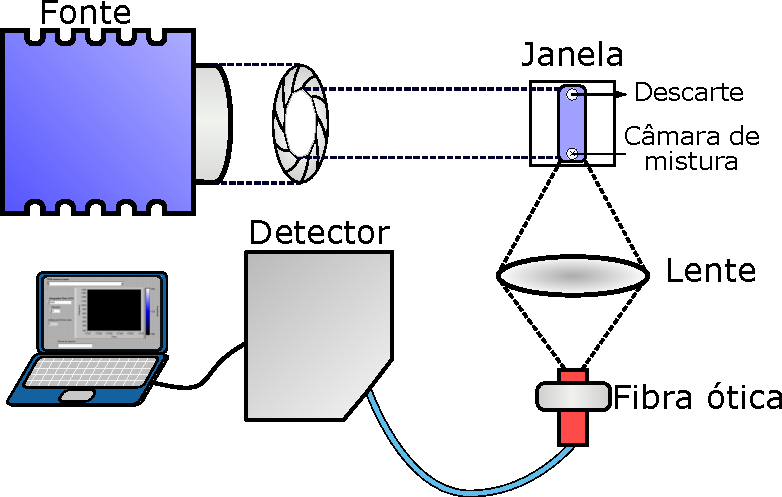
\includegraphics[width=0.7\textwidth]{imagens/fluor/diagrama_stopped_flow_rene}
				\caption{Diagrama mostrando a montagem experimental para os experimentos de fluorescência resolvida no tempo}
				\label{fig:diagrama_stoppedflow_rene}
			\end{figure}
			
			Para a aquisição de dados, utilizou-se um programa escrito em LabView 2013, da National Instruments. O código de aquisição foi escrito pelo Prof. Dr. René Nome e modificado pelo aluno. O painel frontal do programa se encontra na Fig. \ref{fig:fluor_painelfrontal} e o código fonte, na Fig. \ref{fig:fluor_gravacaodados}.
			
			\begin{figure}[h]
				\centering
				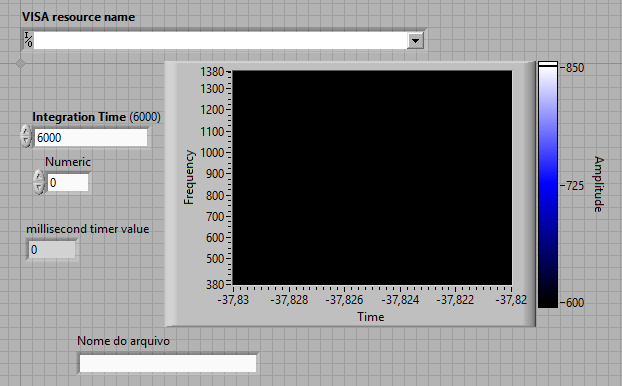
\includegraphics[width=0.7\textwidth]{imagens/fluor/painel_frontal}
				\caption{Painel frontal do programa de aquisição de dados}
				\label{fig:fluor_painelfrontal}
			\end{figure}
			
			\begin{figure}[h]
				\centering
				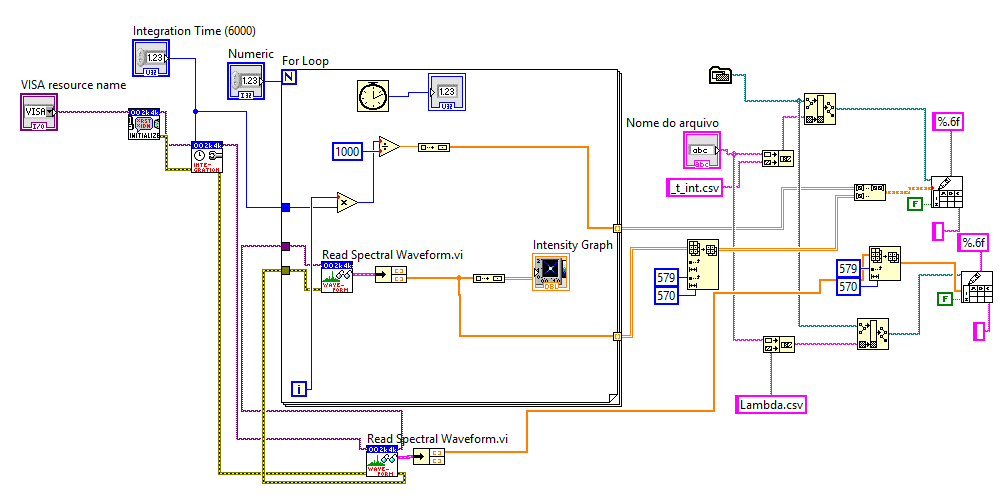
\includegraphics[width=0.7\textwidth]{imagens/fluor/gravacao_dados}
				\caption{Código fonte do programa de aquisição de dados}
				\label{fig:fluor_gravacaodados}
			\end{figure}

			% todo: colocar a pressão
			Após iniciar a aquisição de dados, acionava-se rapidamente o botão de injeção do \emph{stopped-flow}, que empurrava os êmbolos das duas seringas simultaneamente. A pressão utilizada para injeção era de XYZ Pa. Os tempos de integração e o número de pontos de aquisição variavam de acordo com o experimento. O programa gera dois arquivos, um contendo os \(n\) comprimentos de onda de cada ponto medido num vetor coluna (\emph{nome\_t\_int.csv}) e outro continha uma matriz com os \(m \times n\) pontos de aquisição, além dos \(m\) tempos de aquisição, em milissegundos, na primeira coluna (\emph{nome\_t\_int.csv}). A matriz resultante tem tamanho \(m\times n+1\).
			
			Foi criado um mapa de cor para cada matriz. Dessa matriz, extraiu-se a coluna que continha informações do comprimento de onda no máximo do espectro de emissão, em 411 nm, junto com a coluna de tempos. Esse dado, após ser normalizado pelo máximo de intensidade, foi utilizado para realizar as análises quantitativas de cinética. A listagem \ref{lst:extracao_fluor1} mostra o código utilizado para realizar essas tarefas. Esse código foi colocado em um \emph{Jupyter Notebook}, e a cada novo experimento, o nome do arquivo era alterado e todas as tarefas eram aplicadas automaticamente, facilitando muito a visualização ágil dos dados.
			
			\begin{listing}[h]
				\inputminted{python}{./python/fluor_plot_inicial.py}
				\caption{Código fonte para a criação de mapas de cor e extração de informações em 411 nm.}
				\label{lst:extracao_fluor1}
			\end{listing}
			
		\section{Tratamento de dados}  \index{Fluorescência!tratamento de dados}
		
			As informações de intensidade por tempo, em 411 nm, de cada amostra foram plotadas comparativamente. Notou-se que os dados eram bastante ruidosos, mas que havia uma tendência geral. Para facilitar as comparações, aplicou-se o filtro de Savitzky-Golay. Esse filtro ajusta um polinômio de grau \(n\) sobre um conjunto de dados de tamanho ímpar (janela), \(j\). O ponto médio experimental então é substituído pelo ponto médio do ajuste. Para os pontos nas extremidades, onde não há pontos suficientes para o tamanho da janela, utilizou-se o modo padrão do pacote \emph{scipy}, interpolação. Por exemplo, no início da aplicação do filtro, há \(\frac{j}{2}\) pontos à direita mas menos de \(\frac{j}{2}\) pontos à esquerda. Para completar essa falta, é feito um ajuste de grau \(n\) dos primeiros \(j\) pontos, e esse ajuste é estendido para antes do primeiro ponto, garantindo então que existam \(\frac{j}{2}\) à direita e à esquerda do ponto médio.
			
			Utilizou-se dois filtros de segundo grau, mas com tamanhos de janela diferente, para antes e depois da injeção. O ponto de injeção foi determinado manualmente. O tamanho da janela foi escolhido de acordo com o número total de pontos de cada parte. Antes da injeção, utilizou-se como janela o número de pontos, dividido por 2, arredondando para o número inteiro mais próximo, e caso seja ímpar, adicionou-se 1 ao número. Para o conjunto de dados depois da injeção, utilizou-se 201 pontos para conjuntos com 10000 pontos no total e 101 pontos para conjuntos com 5000 pontos. Esses valores foram determinados testando-se várias janelas e escolhendo aquelas com o melhor alisamento.
			
			Após o alisamento, estudou-se o tempo de injeção e a taxa de decaimento após a injeção. O tempo de injeção foi determinado contando-se o número de pontos alisados pertencentes à região de acréscimo de fluorescência. A taxa de decaimento foi determinada realizando-se ajustes monoexponenciais (Eq. \ref{eqn:decaimento_exponencial}) e comparando-se os valores de \(R^2\) (Eq. \ref{eqn:R2}). Outros modelos foram testados, mas o ajuste monoexponencial descrevia muito bem os dados, e era o mais simples.
			
			\begin{equation}
				y = y_0 + A_1 e^{\frac{-x}{t_1}}
				\label{eqn:decaimento_exponencial}
			\end{equation}
			
	\chapter{Técnicas adicionais}
		\section{Calorimetria diferencial de varredura}  \index{calorimetria diferencial de varredura DSC}
		
		Foram realizadas análises utilizando o equipamento institucional DSC Q100 da TA Instruments. O preparo de amostra seguiu as mesmas considerações descritas na seção \ref{sec:reologia_preparo_amostra}. Foram programadas rampas de 2°C/min de 1°C a 60°C, e de volta, com intervalos de 3 minutos na temperatura final.
		
%		\begin{enumerate}[noitemsep]
%			\item Equilíbrio a 1°C
%			\item Rampa até 60°C na taxa de 2°C/min
%			\item Isotérmica por 3 minutos
%			\item Rampa até 1°C na taxa de 2°C/min
%			\item Isotérmica por 3 minutos
%		\end{enumerate}
		
		A análise foi realizada sob fluxo de nitrogênio a 50 ml/min e as massas utilizadas estavam na faixa de 10 a 20 mg. As áreas de transição e temperaturas de transição foram determinadas pelo software do equipamento. As larguras a meia-altura foram determinadas de acordo com o script as listagens \ref{lst:meia_altura1} e \ref{lst:meia_altura2}.
		
		\begin{listing}[h]
			\inputminted{python}{./python/meia_altura1.py}
			\caption{Código fonte para o script de obtenção dos valores de largura a meia altura de curvas de DSC (1/2)} 
			\label{lst:meia_altura1}
		\end{listing}
		
		\begin{listing}[h]
			\inputminted{python}{./python/meia_altura2.py}
			\caption{Código fonte para o script de obtenção dos valores de largura a meia altura de curvas de DSC (2/2)} 
			\label{lst:meia_altura2}
		\end{listing}

		\section{Espalhamento dinâmico de luz} \index{espalhamento dinâmico de luz DLS}
		
		% todo: colocar mais detalhes experimentais aqui.
		Foram realizadas análises de espalhamento dinâmico de luz no Malvern ZetasizerNano Zs-Zen3600 com o objetivo de observar o tamanho dos objetos das amostras de surfactante e ureia acima da temperatura de transição. Desse modo, a temperatura de análise foi fixada em 50°C e as amostras foram termostatizadas nessa temperatura por 10 minutos antes das medidas. As medidas foram realizadas em triplicata.
		
		\section{Tensiometria} \index{tensiometria}
		
		% todo: checar o diâmetro da agulha.
		Para a determinação do parâmetro de Gordon das misturas aquosas binárias, mediu-se a tensão superficial no equipamento Attension Theta da Biolin Scientific pelo método da gota pendente. Preparou-se misturas com composições e densidades conhecidas, e certificou-se de que estavam homogêneas. Utilizou-se uma agulha com 0,7mm de diâmetro, previamente limpa. A câmera foi focada na agulha e foi calibrada utilizando-se o diâmetro conhecido da mesma. Os parâmetros da câmera foram ajustados pelo método automático. A temperatura da sala onde foram realizadas as medidas era de 18°C. Após confirmação de que os parâmetros de análise estão corretos, medindo-se a tensão superficial de água, iniciou-se as medidas das amostras. Gerava-se uma gota com o maior volume possível de líquido, de modo que a gota estivesse na iminência de cair. Em seguida, iniciou-se a captura de fotos pela câmera, a 12 fotos por segundo, por 10 segundos. Em seguida, cada frame individual foi ajustado pelo método de Young-Laplace de modo a obter um valor de tensão superficial, corrigido pela densidade do líquido. Os valores de tensão superficial foram somados, e considerou-se o desvio padrão dessas medidas como o erro experimental. Esse processo foi repetido cinco vezes por amostra.
\part{Efeito dos aditivos hidrofílicos}
	\label{sec:efeito_aditivos_hidrofilicos} 

	\chapter{Resultados reológicos e calorimétricos}
		
	Esta é a parte principal desta tese, na qual houve uma dedicação prolongada. Aqui, pesquisou-se sobre efeitos dos aditivos hidrofílicos no comportamento das micelas gigantes. Parte dos resultados foram publicados na revista \emph{Journal of Colloid and Interface Science}, sob o título ``\emph{Rheological and calorimetric study of alkyltrimethylammonium bromide-sodium salicylate wormlike micelles in aqueous binary systems}"\cite{Clinckspoor2018}.
	
	A inspiração para a glicerina e o DMSO vieram de estudos de outras áreas, onde se mostrou que ambos possuíam a capacidade de melhorar o armazenamento criogênico de células animais, como hemácias e esperma\cite{Butler1959, Polge1949}, sendo que essa propriedade do DMSO está relacionada à sua capacidade de permear membranas\cite{Notman2006}. Logo, se esses aditivos foram capazes de preservar células vivas após o congelamento, qual seria seu efeito em sistemas de autoassociação? Desse tipo de questionamento vieram os estudos de Hoffmann\cite{Grabner2014, Song2008a, Shinto2012}. Em seguida, \citeauthor{Abdel-Rahem2014} utilizou o 1,3-butanodiol, devido às suas aplicações como aditivo para fixar fragrâncias e agente antimicrobiano. A sacarose foi escolhida, devido à similaridade de suas interações com a água, e à similaridade da constante dielétrica, com a glicerina, e por já ter sido estudada anteriormente, com lamelas.\cite{Song2008a} Por último, a ureia é um aditivo frequentemente descrito como agente desestruturante da água, que leva à desnaturação de proteínas, aumenta a solubilidade de hidrocarbonetos e inibe a agregação micelar.\cite{Kuharski1984} Seguindo a hipótese de \citeauthor{Hoffmann2010}, esses aditivos, apesar de serem diferentes estruturalmente, deveriam resultar em efeitos nos perfis de viscosidade, e possivelmente nas outras técnicas, caso seus índices de refração sejam semelhantes. 
	
	Serão apresentados inicialmente os resultados de curva de fluxo (\autoref{sec:efeito_aditivos_viscosidade}). Em conjunto, serão apresentados os resultados calorimétricos, tanto de formação de micelas gigantes (\autoref{sec:efeito_aditivos_calorimetria_mg}) quanto de formação de micelas esféricas (\autoref{sec:efeito_aditivos_calorimetria_me}). Em seguida, serão levantados alguns parâmetros que podem ser utilizados para descrever o efeito dos aditivos (\autoref{sec:efeito_aditivos_viscosidade}). Os resultados calorimétricos serão correlacionados aos parâmetros (\autoref{sec:correlacao_params_cmc_dh}). Como complemento aos estudos com as curvas de fluxo, será avaliada a reologia oscilatória (\autoref{sec:reologia_oscilatoria}), e, como será mostrado, a ureia possui um efeito muito diferente, e será estudado mais a fundo no \autoref{sec:cap_efeito_ureia}.
	
	Como base para a discussão, utilizou-se a concentração dos aditivos em fração mássica (\% m/m). Isso se deve porque é a base de concentração utilizada na literatura da área, e os bancos de dados possuem as propriedades geralmente em função dessa grandeza. O \autoref{sec:tabelas_conversao} contém algumas tabelas convertendo a fração mássica para outras grandezas de concentração, como molaridade, molalidade, fração molar e proporções molares.

	
		\section{Efeitos dos aditivos na viscosidade do repouso} \index{resultados!efeito do solvente}
			\label{sec:efeito_aditivos_viscosidade} \index{resultados!índice de refração} \index{resultados!índice de refração}
			A reologia é uma técnica que pode fornecer informações sobre a dinâmica de relaxação de um material, através da viscosidade. Em especial, o perfil de viscosidade em repouso \(\eta_0\) (\autoref{fig:regioes_rh}) está relacionado com mudanças no processo de relaxação das micelas. Com o intuito de se estudar como a relaxação das micelas é afetada pelos aditivos, foram construídos vários diagramas de viscosidade, sempre com 100 \mM{} de \CTAB, para várias concentrações de aditivo.
			
			Neste momento, os resultados serão discutidos com base somente no índice de refração das soluções, partindo da primeira premissa apresentada na \autoref{sec:efeito_solvente}. Relembrando, essa premissa se baseia na diminuição no valor da constante de Hamaker (\autoref{eqn:constante_hamaker_lifshitz}), que diminui a atração entre as micelas, consequentemente acelerando o mecanismo de reptação, e não afetando o mecanismo de quebra e recombinação (\autoref{fig:regioes_rh}). A \autoref{fig:indice_refracao} mostra como o índice de refração das soluções com os aditivos variam em função da fração mássica de aditivo. A reta horizontal possui o mesmo índice de refração, então aditivos diferentes deveriam ter o mesmo efeito na reologia.
					
			\begin{figure}[h]
				\centering
				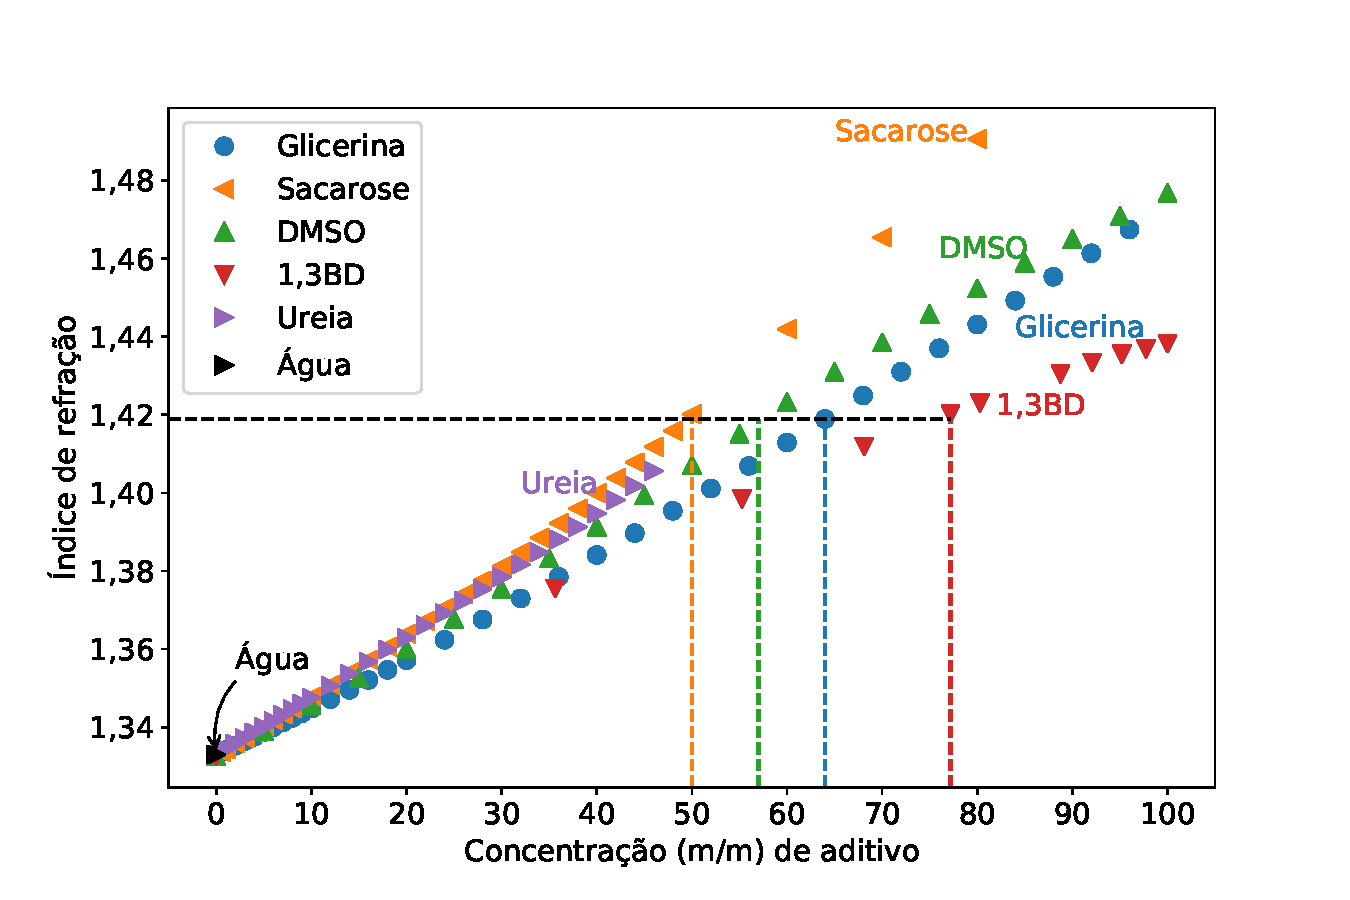
\includegraphics[width=0.7\textwidth]{imagens/propriedades/indice_refracao}
				\caption{Índice de refração  em função da concentração de glicerina, sacarose e ureia a 20°C\cite{Lide2003}, e de DMSO\cite{Lebel1962} e 1,3-butanodiol\cite{Piekarski1995} a 25°C. Na linha horizontal, as amostras dos aditivos teriam o mesmo índice de refração, e deveriam possuir o mesmo efeito na constante de Hamaker.}
				\label{fig:indice_refracao}
			\end{figure} \index{propriedades!índice de refração \(n\)}
	
			Inicialmente, comparou-se glicerina com sacarose, devido às suas semelhanças no índice. A \autoref{fig:rh_sacarose_glicerina} mostra os diagramas de viscosidade, em concentrações crescentes de glicerina, e no ponto de igualdade no índice de refração de sacarose, 50\%. Em seguida, notou-se que \BD{} e DMSO possuiam efeitos semelhantes, como mostra a \autoref{fig:rh_13bd_dmso}. Por último, a ureia mostrou um comportamento muito diferente dos outros aditivos (\autoref{fig:rh_ureia}).
			
			\begin{figure}[htb]
				\centering
				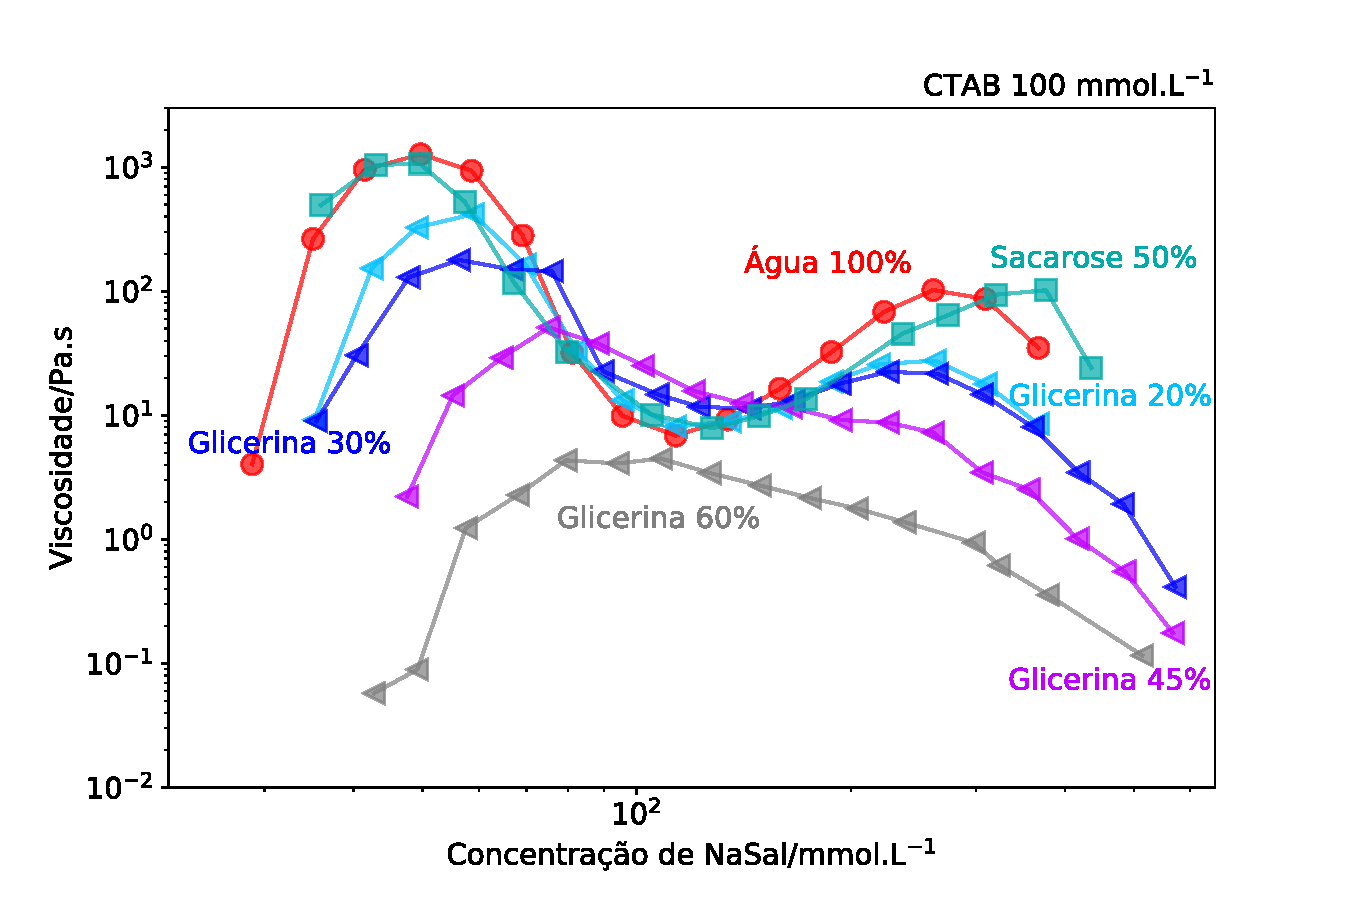
\includegraphics[width=0.7\textwidth]{imagens/reologia/RH_sacarose_glicerina}
				%\caption[Diagrama de viscosidade para glicerina e sacarose]{Viscosidade no repouso \(\eta_0\) em função da concentração de salicilato de sódio (NaSal) em várias concentrações dos aditivos glicerina e sacarose. 60\% de glicerina (V/V) e 50\% de sacarose (m/m) estão no ponto de equivalência do índice de refração. As curvas com 30, 45 e 60 \% de glicerina foram obtidas pela aluna de mestrado Laila Lorenzetti, coautora do trabalho.}
				\caption{Viscosidade no repouso \(\eta_0\) em função da concentração de salicilato de sódio (NaSal) em várias concentrações dos aditivos glicerina e sacarose.
				%	 A concentração de \CTAB{} é de 100 \mM{}.
					60\% de glicerina (V/V) e 50\% de sacarose (m/m) estão no ponto de equivalência do índice de refração. As curvas com 30, 45 e 60 \% de glicerina foram obtidas pela aluna de mestrado Laila Lorenzetti, coautora do trabalho.}
				\label{fig:rh_sacarose_glicerina}
			\end{figure} \index{resultados!sacarose} \index{resultados!glicerina} \index{resultados!\CTAB}
			
			\begin{figure}[htb]
				\centering
				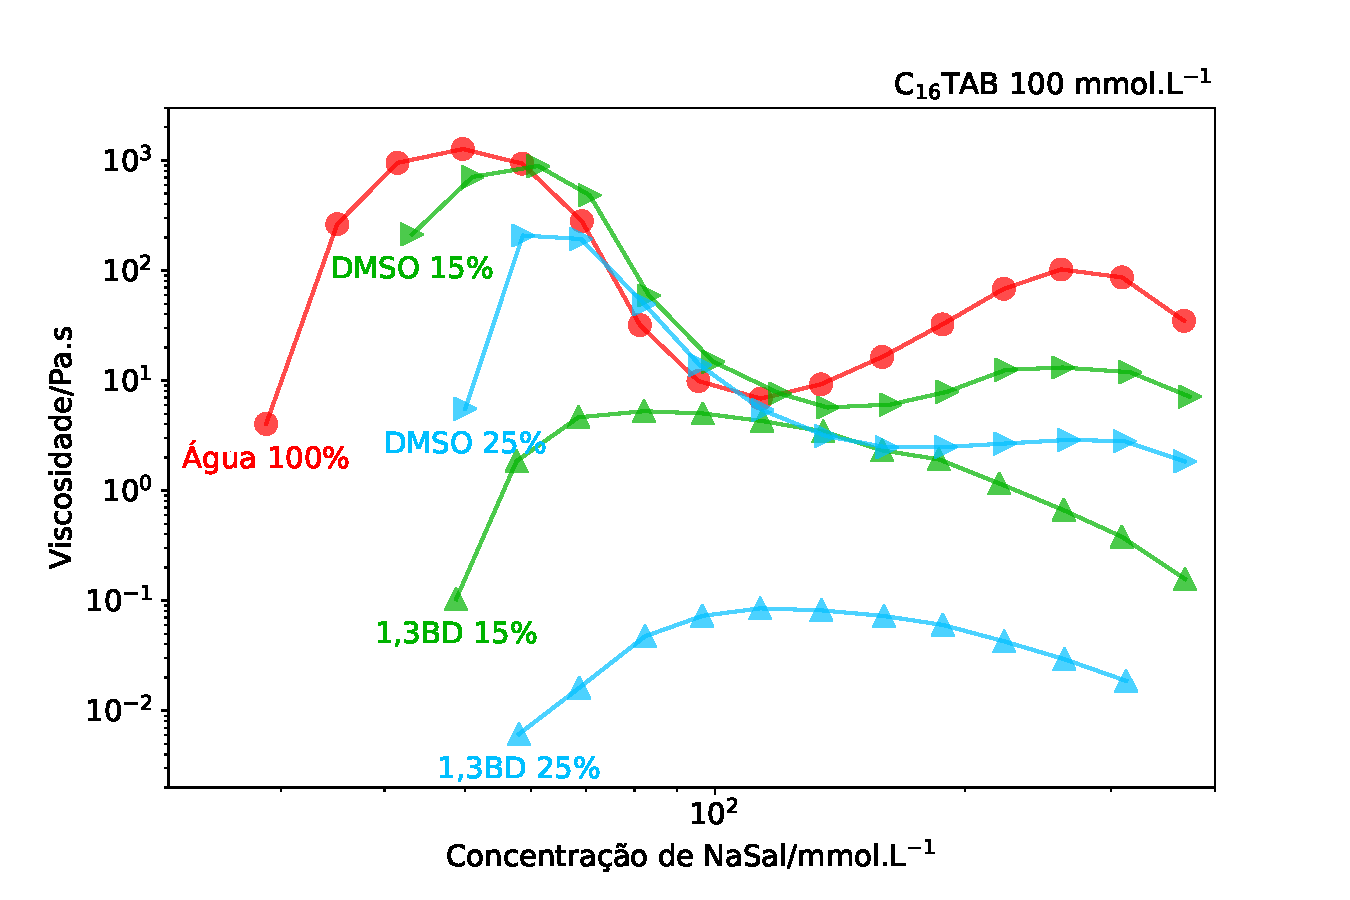
\includegraphics[width=0.7\textwidth]{imagens/reologia/RH_13BD_DMSO}
				%\caption[Diagrama de viscosidade para DMSO e 1,3BD]{Viscosidade no repouso \(\eta_0\) em função da concentração de salicilato de sódio (NaSal) em várias concentrações dos aditivos 1,3-butanodiol (\BD) e dimetilsulfóxido (DMSO). As concentrações de igualdade do índice de refração são 77\% (m/m) e 57\% (m/m), respectivamente}
				\caption{Viscosidade no repouso \(\eta_0\) em função da concentração de salicilato de sódio (NaSal) em várias concentrações dos aditivos 1,3-butanodiol (\BD) e dimetilsulfóxido (DMSO).
					%A concentração de \CTAB{} é de 100 \mM{}.
					As concentrações de igualdade do índice de refração são 77\% (m/m) e 57\% (m/m), respectivamente}
				\label{fig:rh_13bd_dmso}
			\end{figure} \index{resultados!dimetilsulfóxido} \index{resultados!1,3-butanodiol}
			
			\begin{figure}[htb]
				\centering
				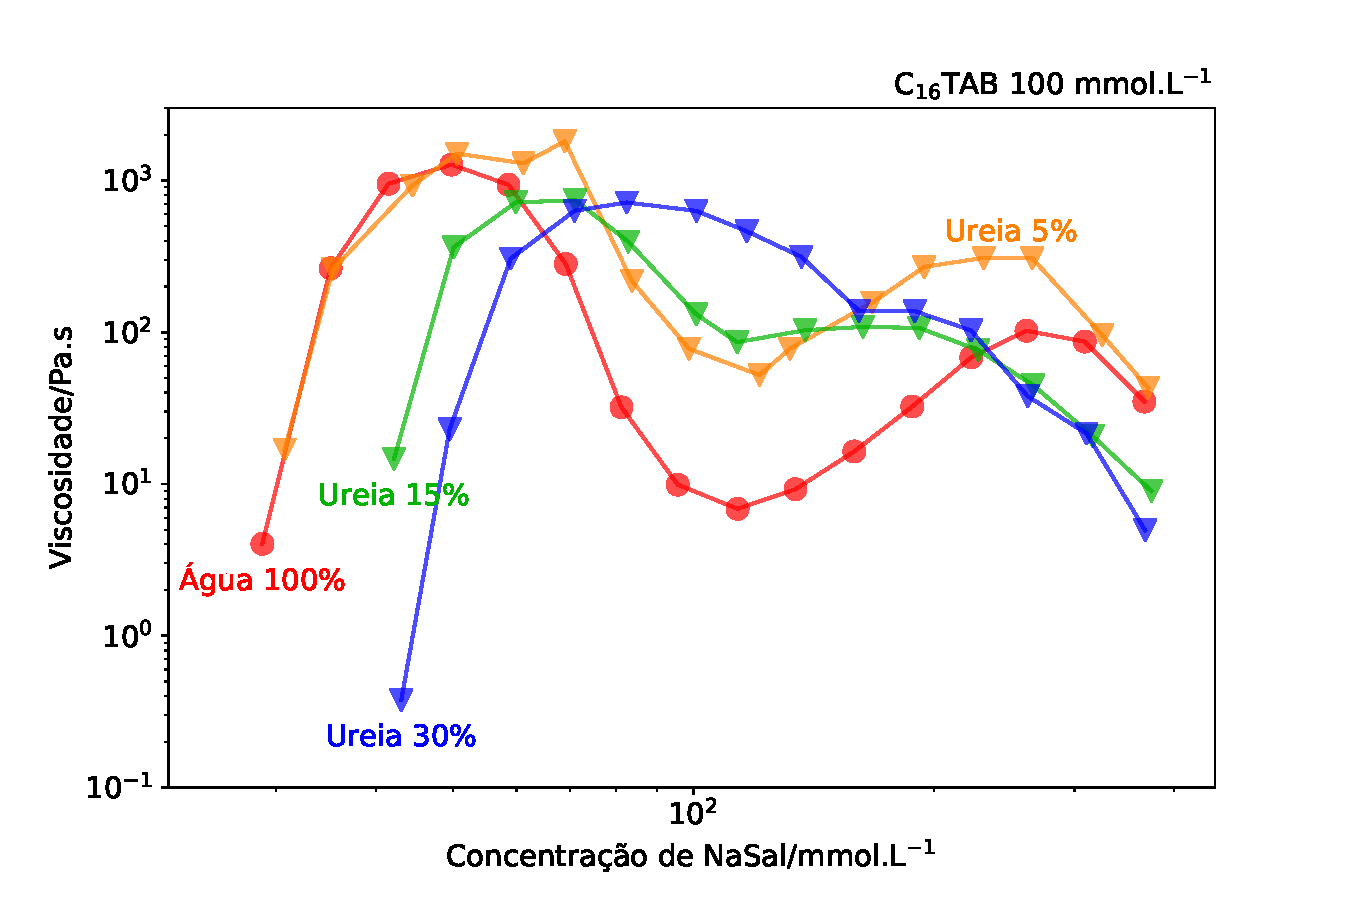
\includegraphics[width=0.7\textwidth]{imagens/reologia/RH_ureia}
				\caption{Viscosidade no repouso \(\eta_0\) em função da concentração de salicilato de sódio (NaSal) em várias concentrações de ureia.
				%	A concentração de \CTAB{} é de 100 \mM{}.
					 A concentração de igualdade de índice de refração é em torno de 55\%.}
				\label{fig:rh_ureia}
			\end{figure} \index{resultados!ureia}
			
			Os dois picos de viscosidade observados em pequenas concentrações de glicerina diminuem, e a região central permanece pouco afetada, como já havia sido observado.\cite{Hoffmann2010} Porém, vemos que a adição de 50\% de sacarose praticamente não afetou a viscosidade das soluções, apesar da igualdade no índice de refração dessas soluções. Isso mostra que considerar somente o índice de refração não permite a previsão do comportamento dessas soluções. O perfil de viscosidade de DMSO e \BD{} foi muito mais afetado pelos aditivos do que era esperado observando-se somente o índice de refração, em especial o 1,3-butanodiol, onde 15\% (m/m) possui o mesmo efeito na viscosidade que 60\% de glicerina. No caso da ureia, a viscosidade na região central aumentou, algo não observado nos outros aditivos, porém o perfil é semelhante a outro já observado em água, com orto-hidróxicinamato e \CTAB{} em pH 9. \cite{Clinckspoor2015}
			
		\FloatBarrier
		
		\section{Efeito dos aditivos na calorimetria de micelas gigantes} \index{resultados!ITC} \index{resultados!\TTAB}
		\label{sec:efeito_aditivos_calorimetria_mg}
			A calorimetria de titulação isotérmica fornece informações sobre o quão favorável é a formação das micelas, através da concentração de formação de micelas gigantes, \cwlm. As Figuras \ref{fig:itc_mg_glicerina}, \ref{fig:itc_mg_sacarose}, \ref{fig:itc_mg_13bd}, \ref{fig:itc_mg_dmso} e \ref{fig:itc_mg_ureia} mostram os perfis de formação de micelas gigantes para glicerina, sacarose, 1,3-butanodiol, dimetilsulfóxido e ureia, respectivamente. 
		
			\begin{figure}[h]
				\centering
				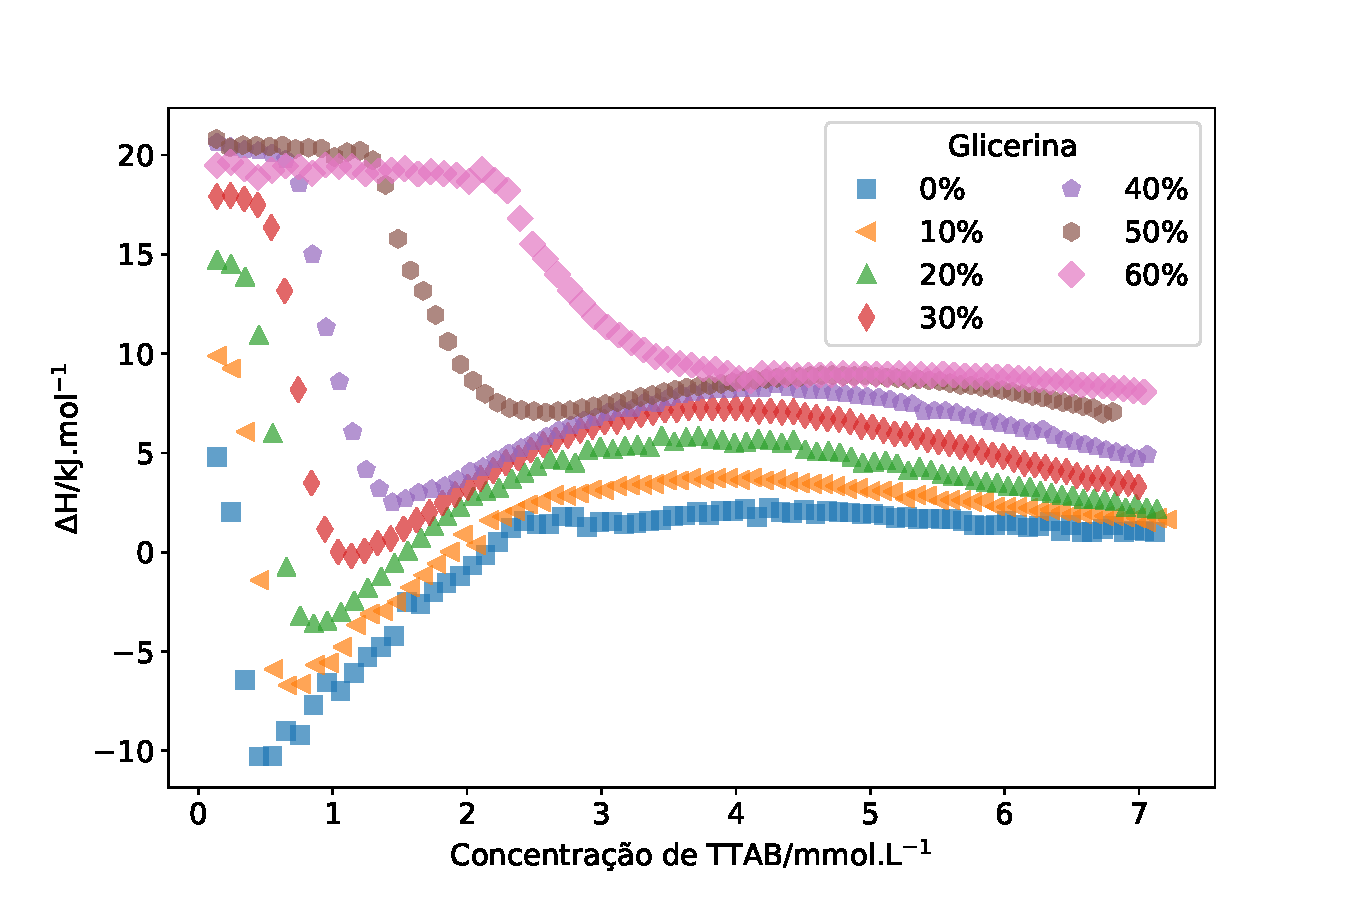
\includegraphics[width=0.7\textwidth]{imagens/itc/ITC_MG_glic}
				\caption{Efeito da concentração de glicerina nas curvas de titulação de formação de micelas gigantes. A concentração de salicilato de sódio na cela de amostra é de 1,5 \mM. A concentração do aditivo está em \% (V/V).}
				\label{fig:itc_mg_glicerina}
			\end{figure}  \index{resultados!glicerina}
			
			\begin{figure}[h]
				\centering
				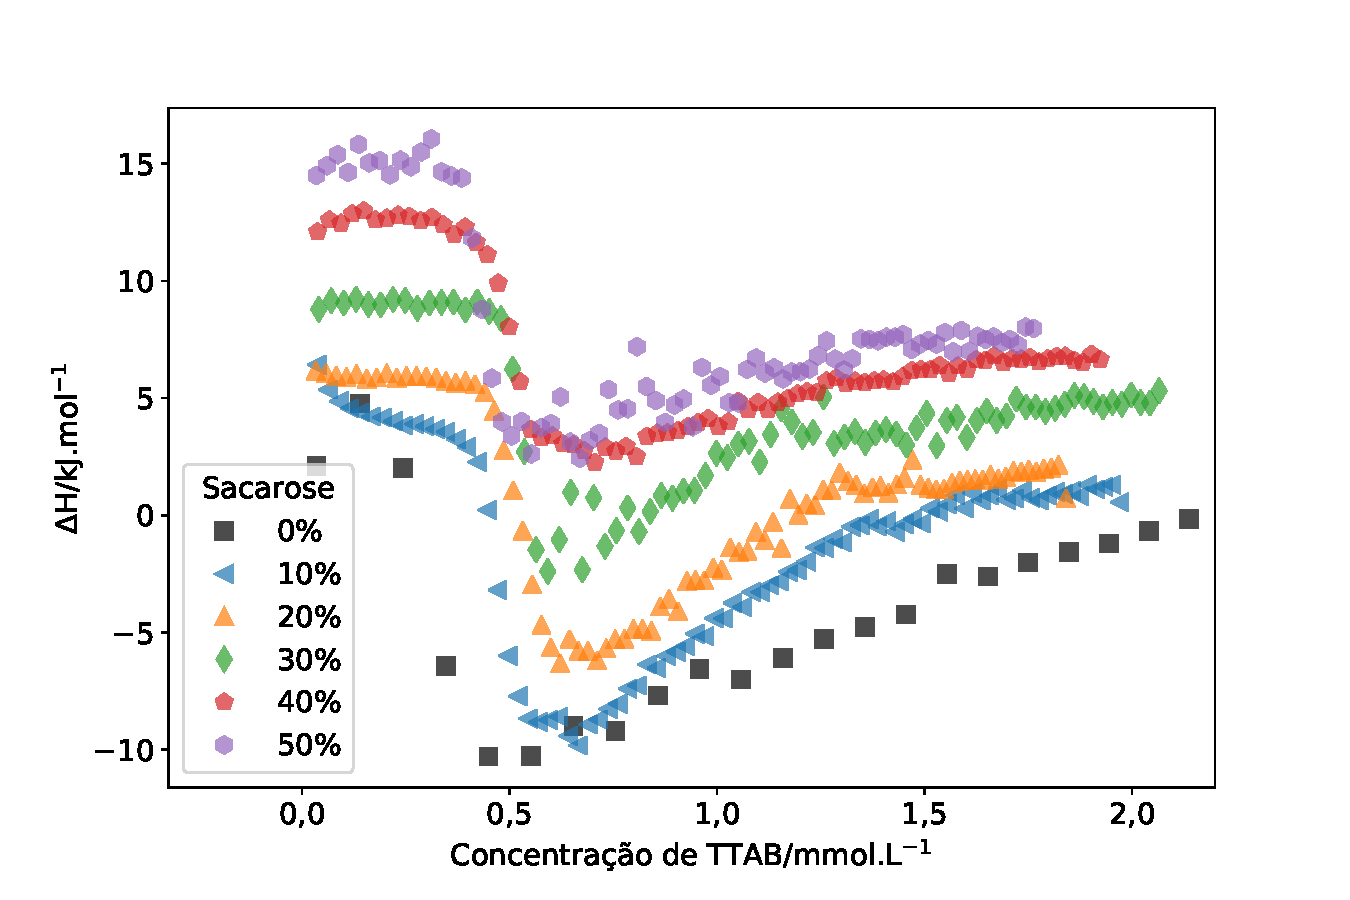
\includegraphics[width=0.7\textwidth]{imagens/itc/ITC_MG_sac}
				\caption{Efeito da concentração de sacarose nas curvas de titulação de formação de micelas gigantes. A concentração de salicilato de sódio na cela de amostra é de 1,5 \mM. A concentração do aditivo está em \% (m/m).}
				\label{fig:itc_mg_sacarose}
			\end{figure} \index{resultados!sacarose}
			
						
			\begin{figure}[h]
				\centering
				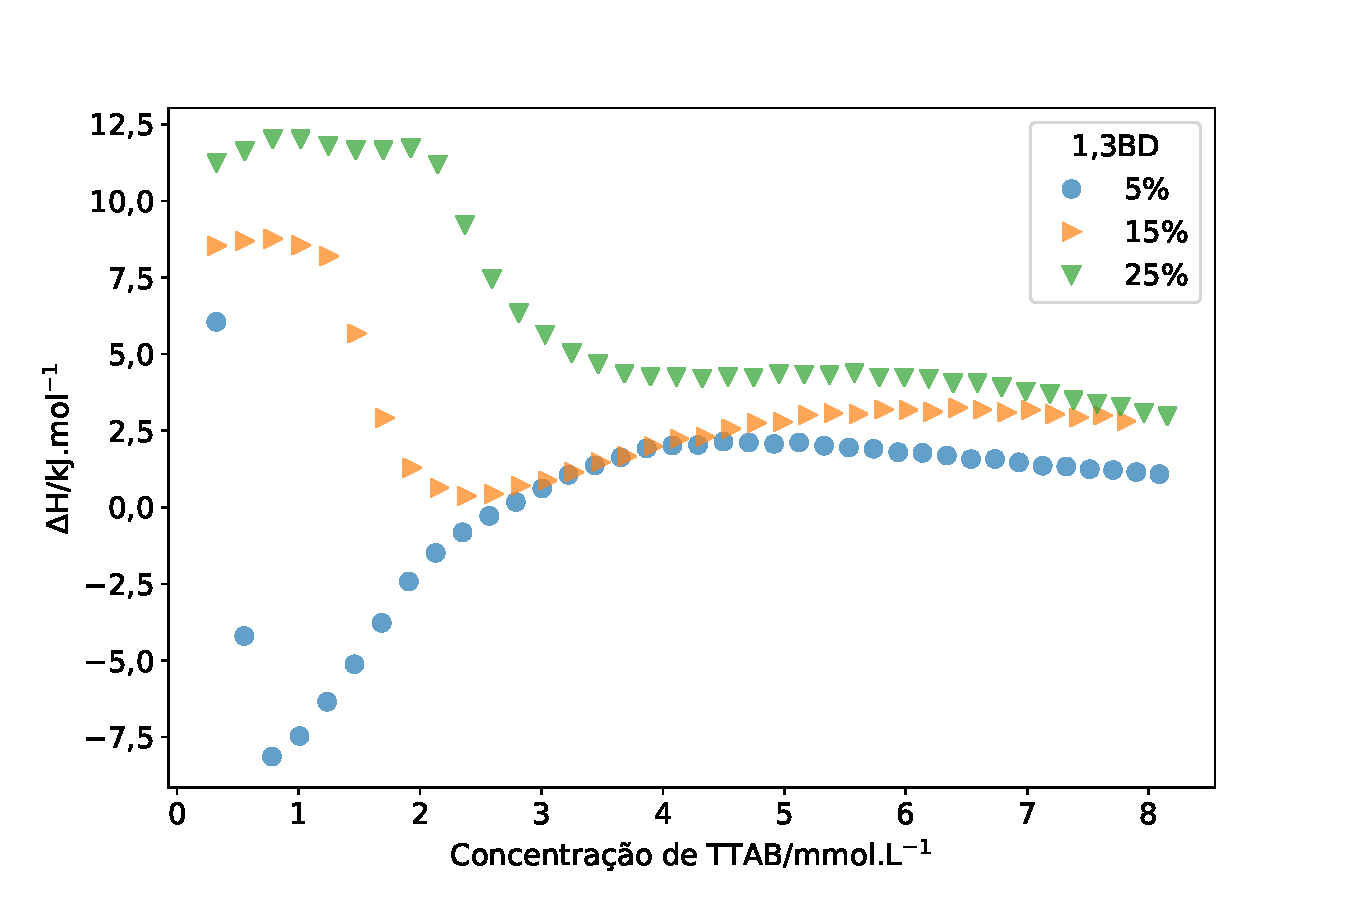
\includegraphics[width=0.7\textwidth]{imagens/itc/ITC_MG_13BD}
				\caption{Efeito da concentração de 1,3-butanodiol nas curvas de titulação de formação de micelas gigantes. A concentração de salicilato de sódio na cela de amostra é de 1,5 \mM. A concentração do aditivo está em \% (m/m).}
				\label{fig:itc_mg_13bd}
			\end{figure} \index{resultados!1,3-butanodiol}
			
			\begin{figure}[h]
				\centering
				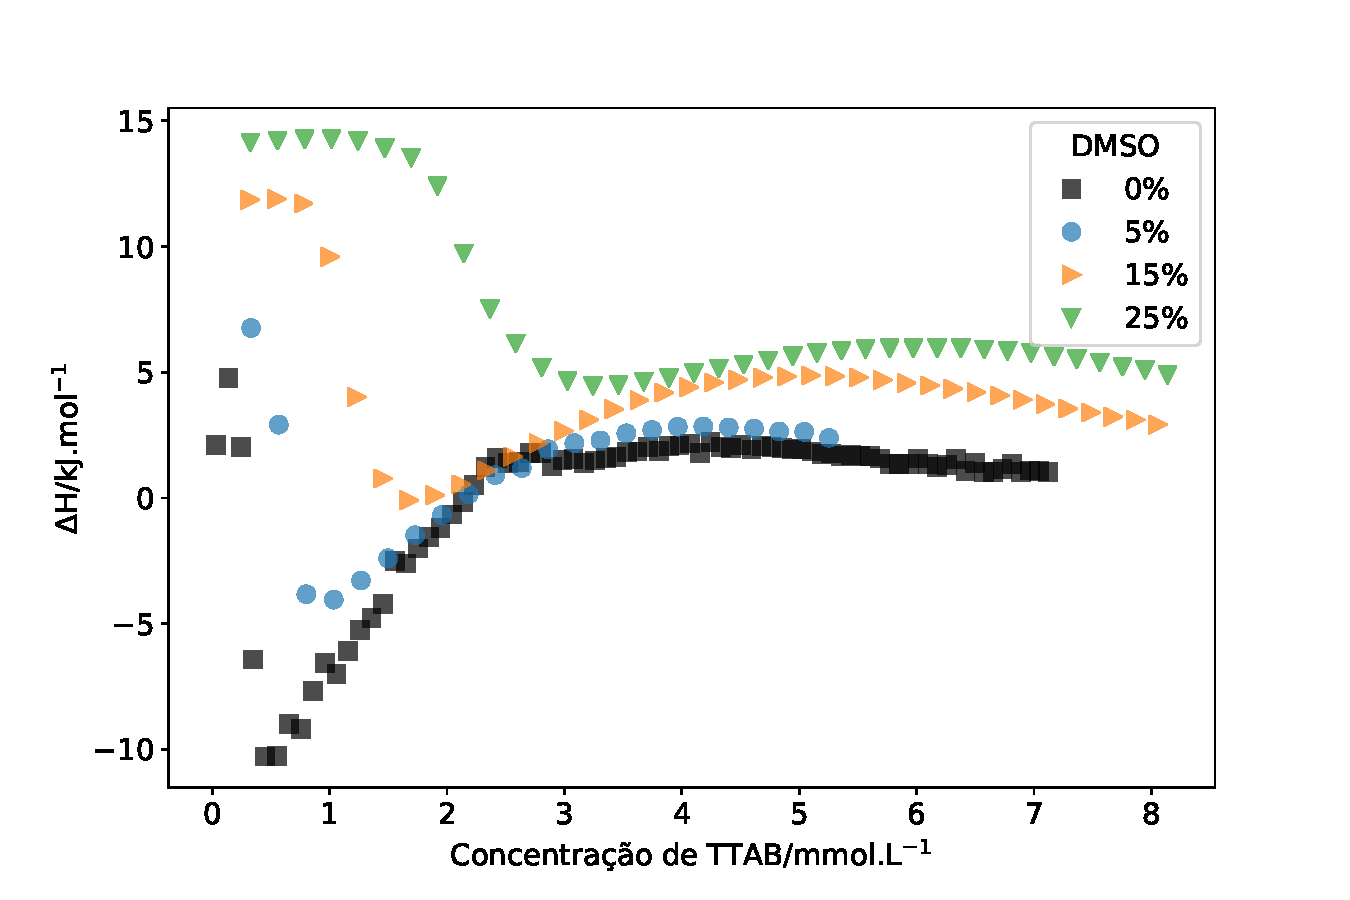
\includegraphics[width=0.7\textwidth]{imagens/itc/ITC_MG_dmso}
				\caption{Efeito da concentração de dimetilsulfóxido nas curvas de titulação de formação de micelas gigantes. A concentração de salicilato de sódio na cela de amostra é de 1,5 \mM. A concentração do aditivo está em \% (m/m).}
				\label{fig:itc_mg_dmso} \index{resultados!dimetilsulfóxido}
			\end{figure}

			\begin{figure}[h]
				\centering
				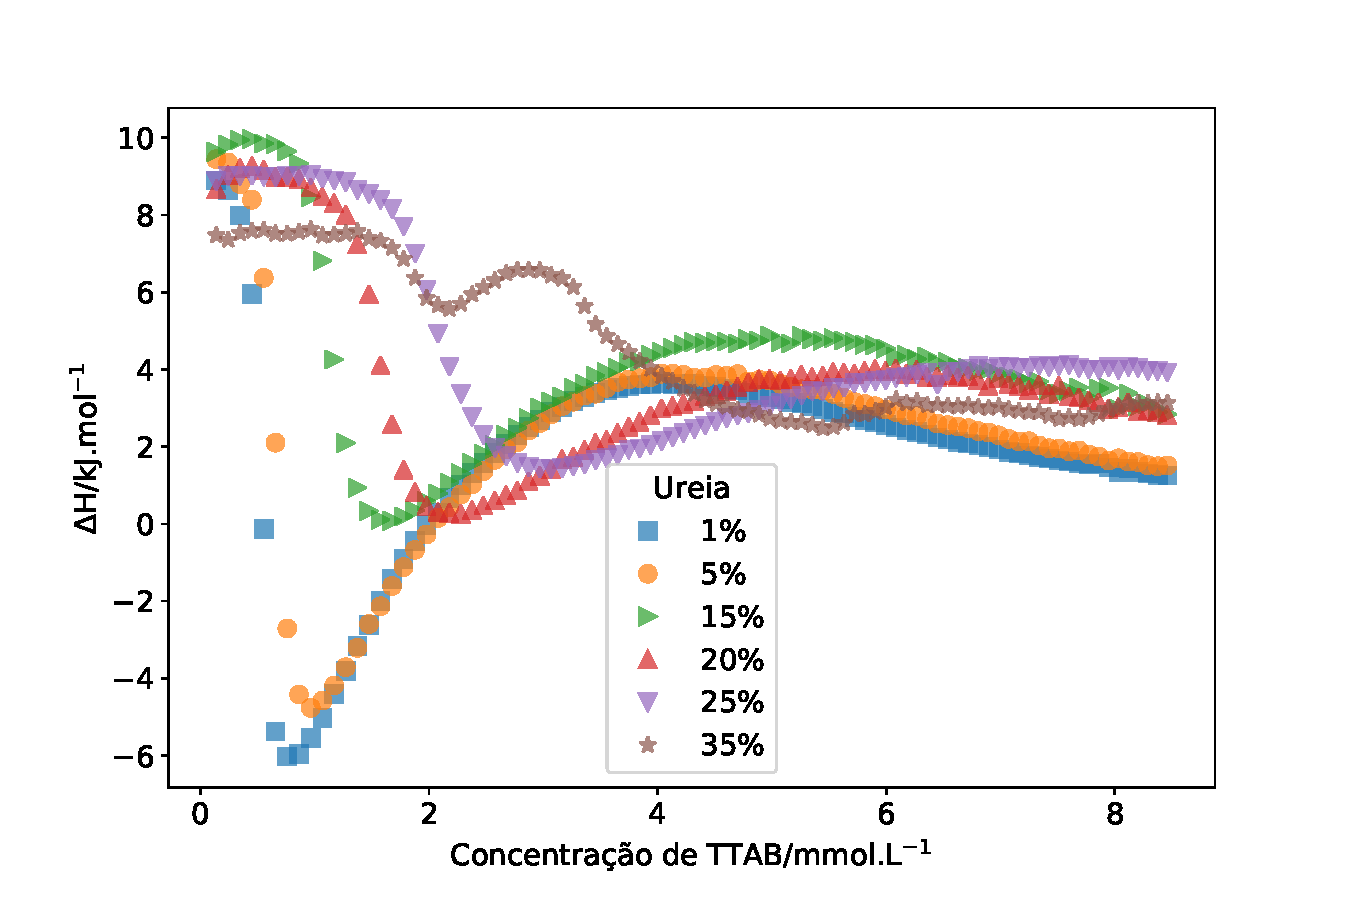
\includegraphics[width=0.7\textwidth]{imagens/itc/ITC_MG_ur}
				\caption{Efeito da concentração de ureia nas curvas de titulação de formação de micelas gigantes. A concentração de salicilato de sódio na cela de amostra é de 1,5 \mM. A concentração do aditivo está em \% (m/m).}
				\label{fig:itc_mg_ureia}
			\end{figure} \index{resultados!ureia}
			
			
			As diferenças entre glicerina e sacarose, novamente, se evidenciaram. Da mesma maneira que na reologia, a presença de sacarose não afetou a formação de micelas gigantes. Já a glicerina teve um efeito deletério na autoassociação, aumentando significativamente a concentração necessária para o crescimento. \BD{} e DMSO não se mostraram muito diferentes, apesar dos perfis reológicos serem bastante distintos, algo não totalmente inesperado, já que ambas as técnicas observam fenômenos diferentes. Isso indica que o \BD{} não leva à uma diminuição na estabilidade micelar, o que poderia levar à uma diminuição na quantidade de micelas, que poderia diminuir a viscosidade dos sistemas. Logo, o \BD{} possui outros mecanismos que afetam as micelas.

			O comportamento da ureia seguiu o esperado, de acordo com a literatura\cite{Souza2012, Bruning1961}, com um aumento de \cwlm{}. É interessante notar que o \DHwlm{} diminui com o aumento da concentração de ureia, o que sugere uma diminuição na adsorção de salicilato nas micelas. Em 35\% de ureia observa-se um perfil bastante diferente dos outros, porém nessa situação, ocorre a formação de um precipitado, cuja natureza será discutida na \autoref{sec:cap_efeito_ureia}.
			
			Uma maneira de se resumir as curvas calorimétricas é utilizando somente a concentração de formação de micelas gigantes (\cwlm) e a entalpia de micelização (\DHwlm). Dessa forma, podemos comparar o efeito da concentração dos aditivos nas curvas mais facilmente, como mostra a \autoref{fig:cwlm_dhwlm_por_conc}. Esse tipo de figura, utilizando outras propriedades na abcissa, será utilizado para realizar novas comparações futuramente.
			
%			\begin{figure}[h]
%				\begin{subfigure}[t]{0.5\textwidth}
%					\centering
%					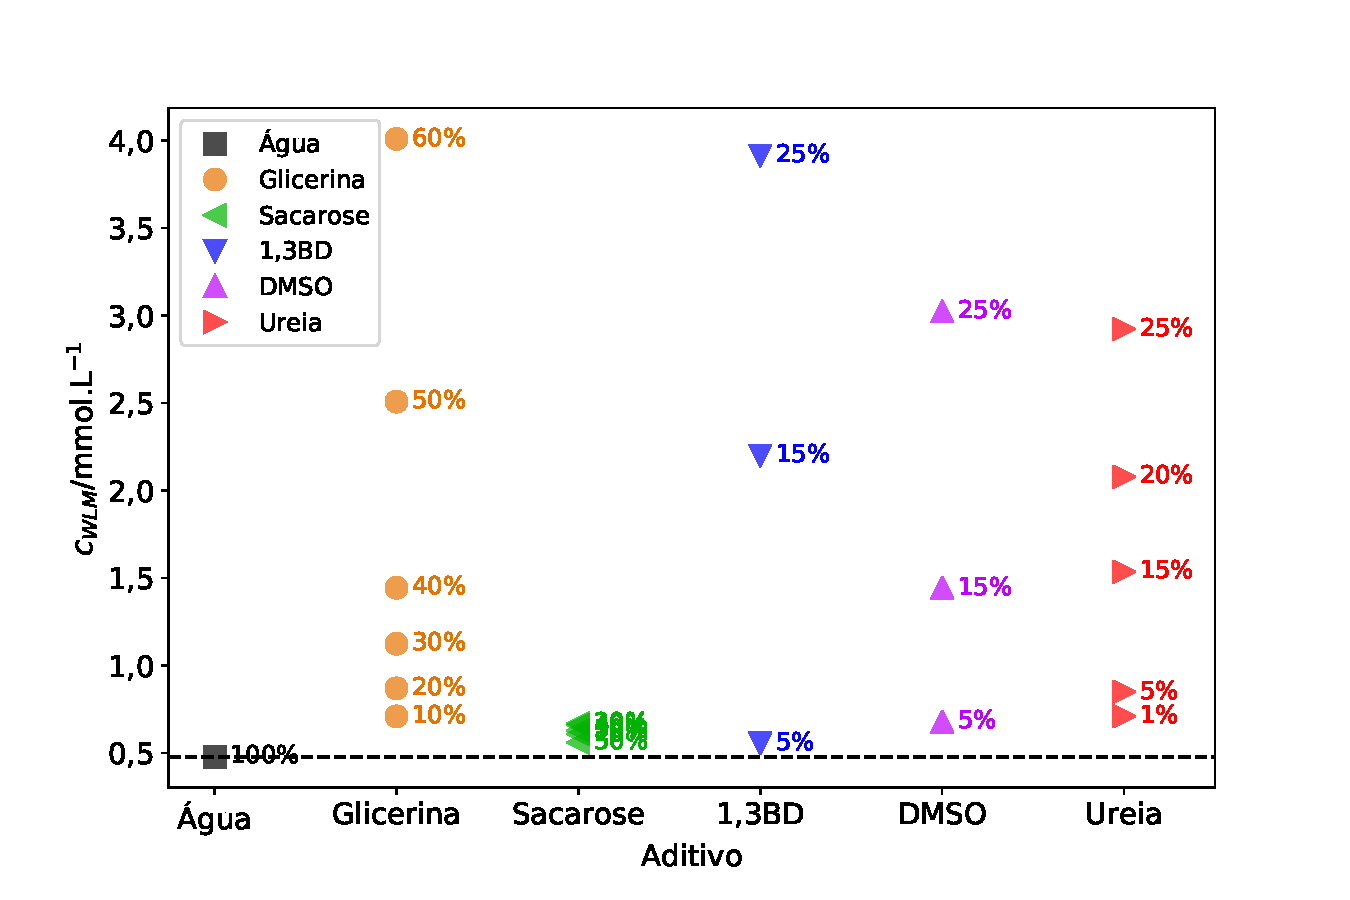
\includegraphics[width=\textwidth]{imagens/itc/Cwlm_por_Aditivo}
%					\caption{\cwlm{}}
%					\label{fig:cwlm_por_aditivo}
%				\end{subfigure}%
%				\begin{subfigure}[t]{0.5\textwidth}
%					\centering
%					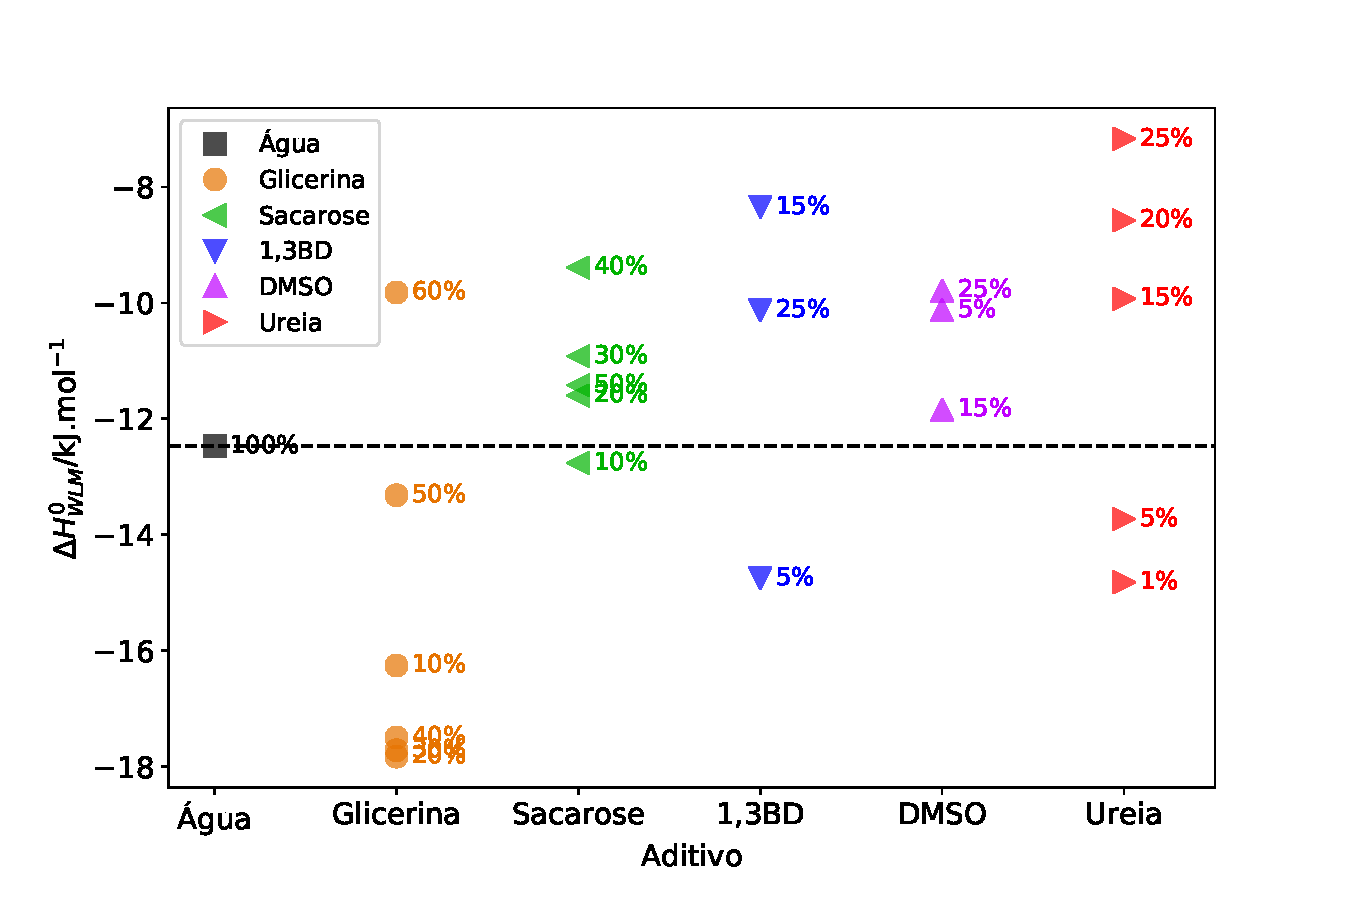
\includegraphics[width=\textwidth]{imagens/itc/DHwlm_por_Aditivo}
%					\caption{\DHwlm{}}
%					\label{fig:dhwlm_por_aditivo}
%				\end{subfigure}
%				\caption{\cwlm{} e \DHwlm{} em função dos aditivos e de sua concentração}
%				\label{fig:cwlm_dhwlm_por_aditivo} % todo: se tiver tempo, alterar o Delta H 0 para Delta H \circ
%			\end{figure} 
		
			\begin{figure}[h]
				\begin{subfigure}[t]{0.5\textwidth}
					\centering
					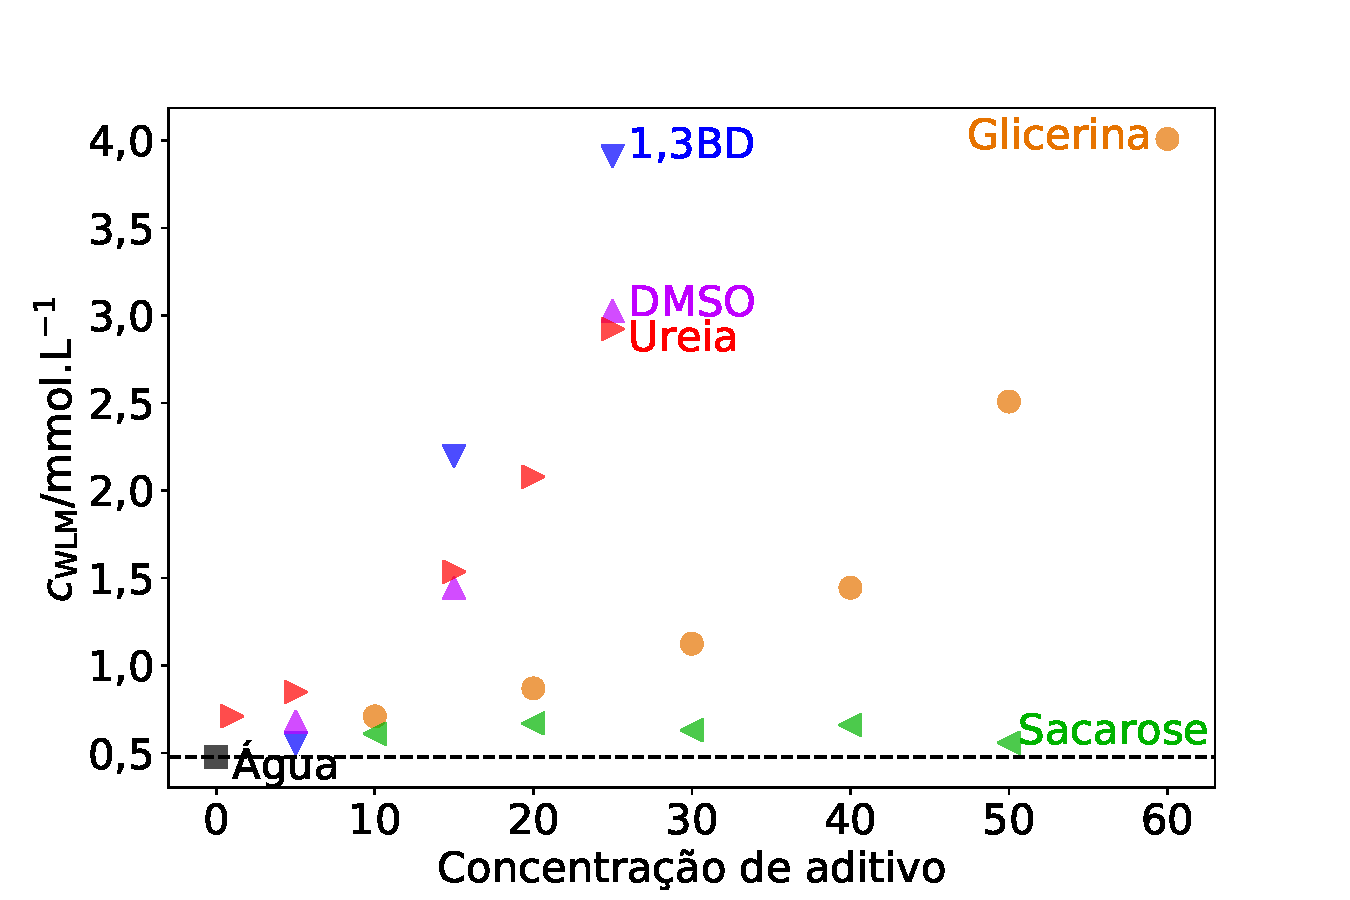
\includegraphics[width=\textwidth]{imagens/itc/Cwlm_por_conc}
					\caption{\cwlm}
					\label{fig:cwlm_por_conc}
				\end{subfigure} %
				\begin{subfigure}[t]{0.5\textwidth}
					\centering
					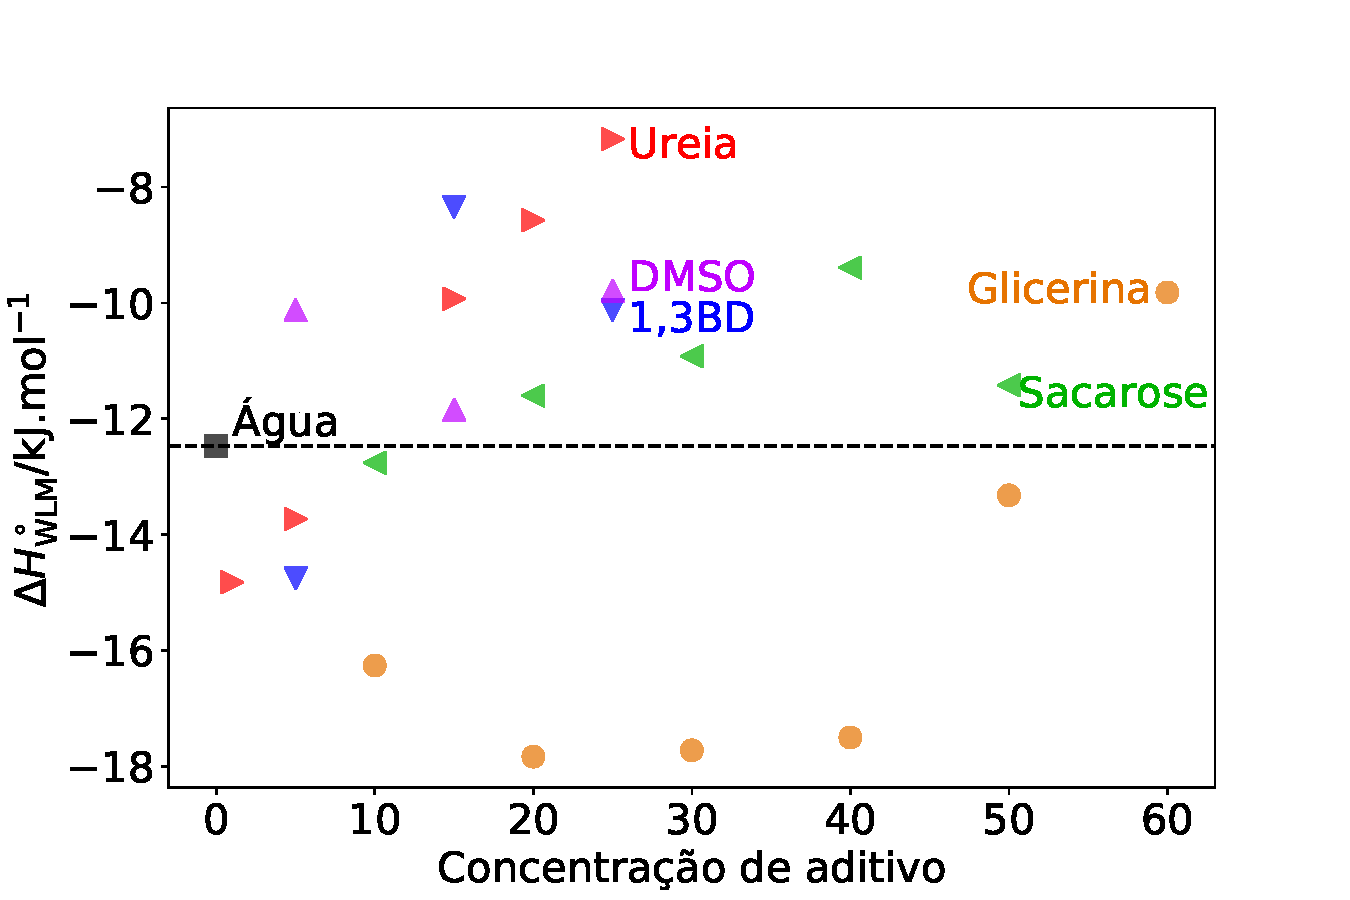
\includegraphics[width=\textwidth]{imagens/itc/DHwlm_por_conc}
					\caption{\DHwlm}
					\label{fig:dhwlm_por_conc}
				\end{subfigure}
				
				\caption{\cwlm{} e \DHwlm{}, obtidas das Figuras \ref{fig:itc_mg_glicerina}---\ref{fig:itc_mg_ureia} em função da concentração de aditivo para titulações de \TTAB{} em NaSal 1,5 \mM.}
				\label{fig:cwlm_dhwlm_por_conc}
			\end{figure}

		Vemos então claramente que os efeitos dos aditivos na \cwlm{} são relativamente bem comportados, com tendências claras para cada aditivo. Já para a \DHwlm, os tendência aparenta ser um pouco caótica, com valores que aumentam e diminuem, como no caso da glicerina.

		\FloatBarrier
		
		\section{Efeito dos aditivos na calorimetria de micelização} \index{resultados!ITC} \index{resultados!\TTAB}
		\label{sec:efeito_aditivos_calorimetria_me}
		A calorimetria de formação de micelas gigantes possui uma complexidade maior devido à presença do salicilato. Para facilitar a interpretação, foram obtidas informações da formação de micelas esféricas, titulando-se \TTAB{} em água. As Figuras \ref{fig:itc_glicerina}, \ref{fig:itc_sacarose}, \ref{fig:itc_13bd}, \ref{fig:itc_dmso} e \ref{fig:itc_ureia} mostram as curvas de titulação para glicerina, sacarose, 1,3-butanodiol, dimetilsulfóxido e ureia, respectivamente.
					
%			\begin{figure}[h]
%				\centering
%				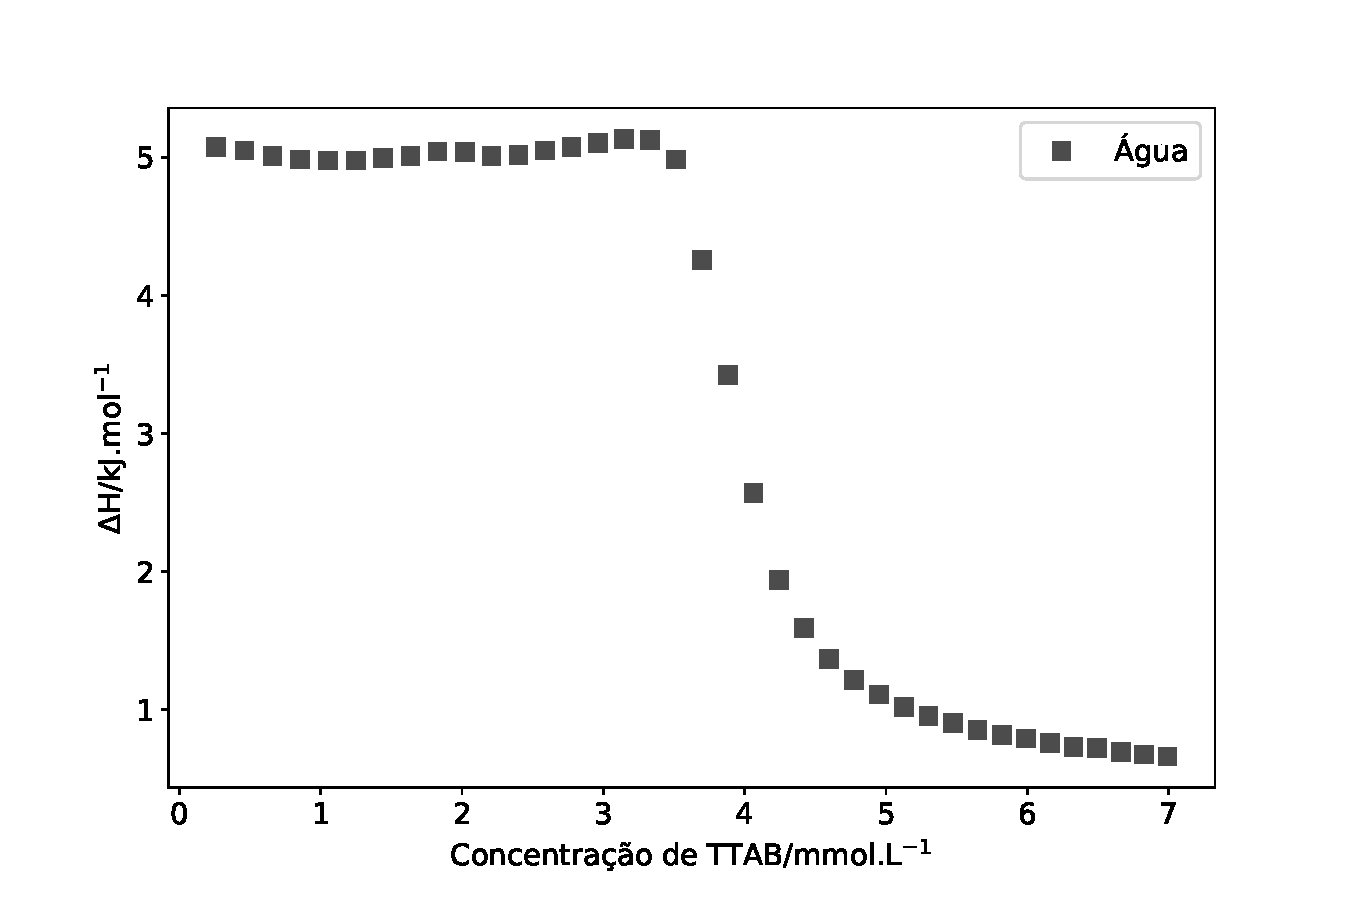
\includegraphics[width=0.7\textwidth]{imagens/itc/ITC_agua}
%				\caption{Titulação de \TTAB em água}
%				\label{fig:itc_agua}
%			\end{figure}
			
			\begin{figure}[h]
				\centering
				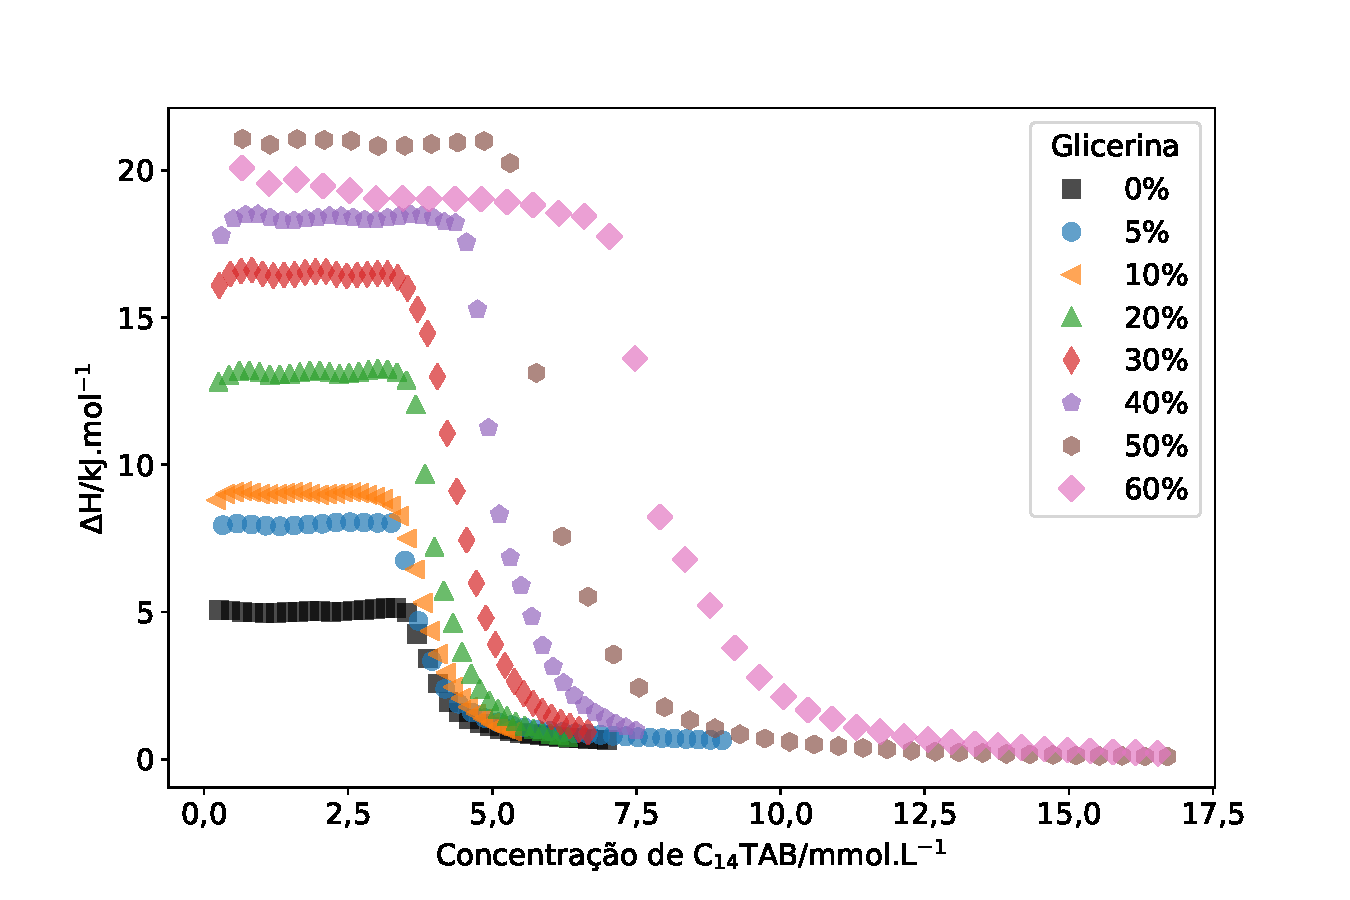
\includegraphics[width=0.7\textwidth]{imagens/itc/ITC_glic}
				\caption{Efeito da glicerina na titulação de \TTAB.}
				\label{fig:itc_glicerina}
			\end{figure} \index{resultados!glicerina}
		
			\begin{figure}[h]
				\centering
				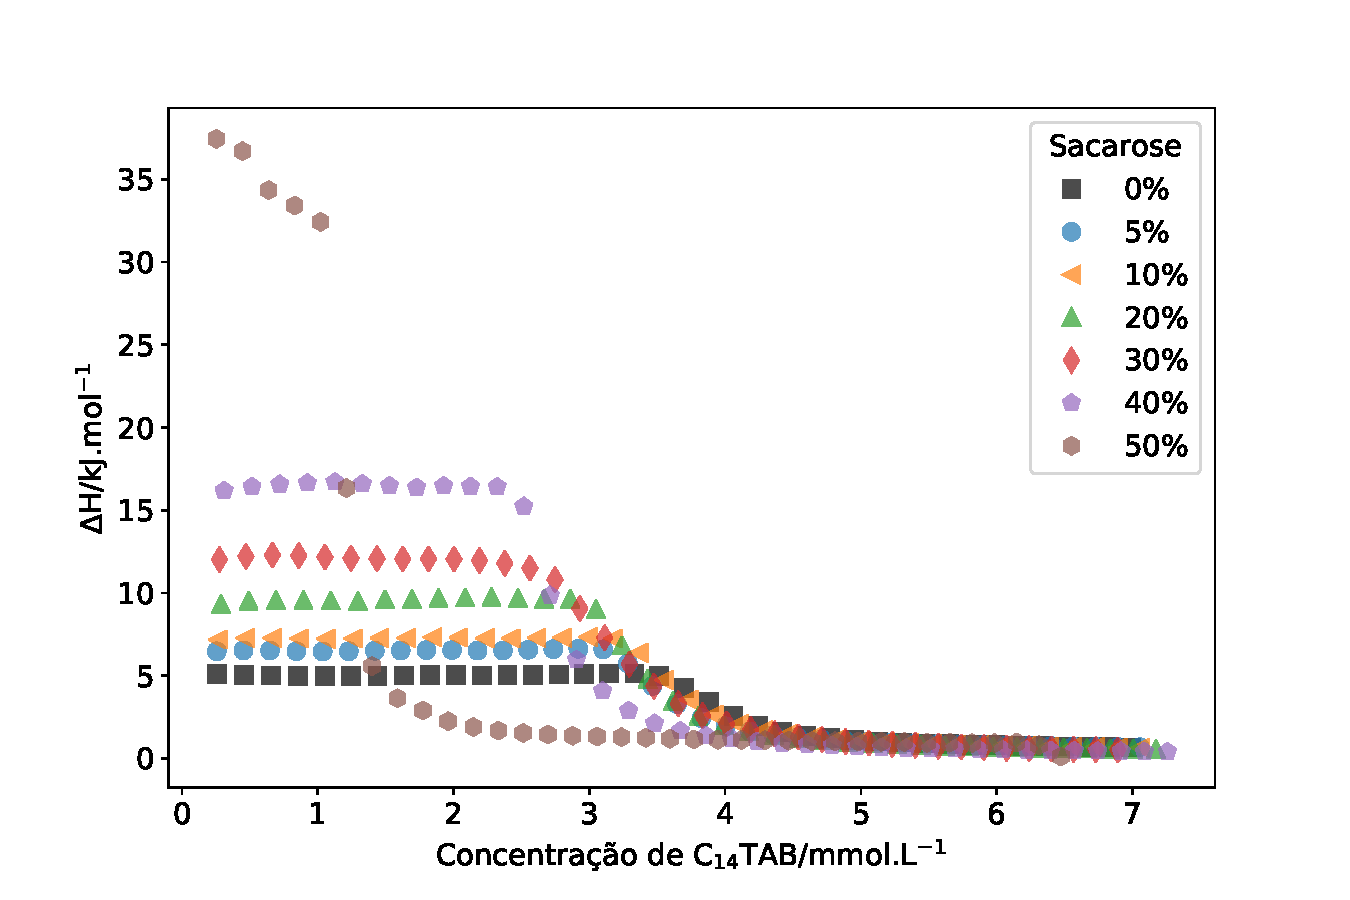
\includegraphics[width=0.7\textwidth]{imagens/itc/ITC_sac}
				\caption{Efeito de sacarose na titulação de \TTAB}
				\label{fig:itc_sacarose}
			\end{figure} \index{resultados!sacarose}
			
			O efeito da glicerina na formação de micelas é semelhante ao efeito em micelas gigantes, exceto pelo aumento do \DHmic{}, na questão da tendência de aumento das concentrações críticas.\cite{Moya2007a} Mais interessante, porém, é que sacarose levou à uma diminuição da \cmc{}. Isso já foi observado para SDS\cite{Bakshi1993a, Chauhan2014}, \CTAB\cite{Banipal2016a} e Brij 35\cite{Sharma1989}. A literatura sugere que a sacarose pode estruturar a água, portanto aumentando a penalidade entrópica e diminuindo a \cmc,\cite{Chauhan2014, Banipal2016a, Sharma1989}, assim como pode interagir com a superfície micelar, diminuindo a repulsão entre as cabeças, estabilizando as micelas.\cite{Bakshi1993a, Chauhan2014, Banipal2016a}. Porém, nas micelas gigantes, o grupo carboxilato do salicilato se encontra nessa mesma região, então há uma competição entre hidroxilas e carboxilatos. Como o carboxilato é carregado, interage mais fortemente com as micelas e impede que a sacarose exerça sua influência estabilizadora, logo não afeta as micelas. O efeito do aumento do índice de refração pode ter sido contrabalanceado pela estruturação do solvente, neste caso.
			
			\begin{figure}[h]
				\centering
				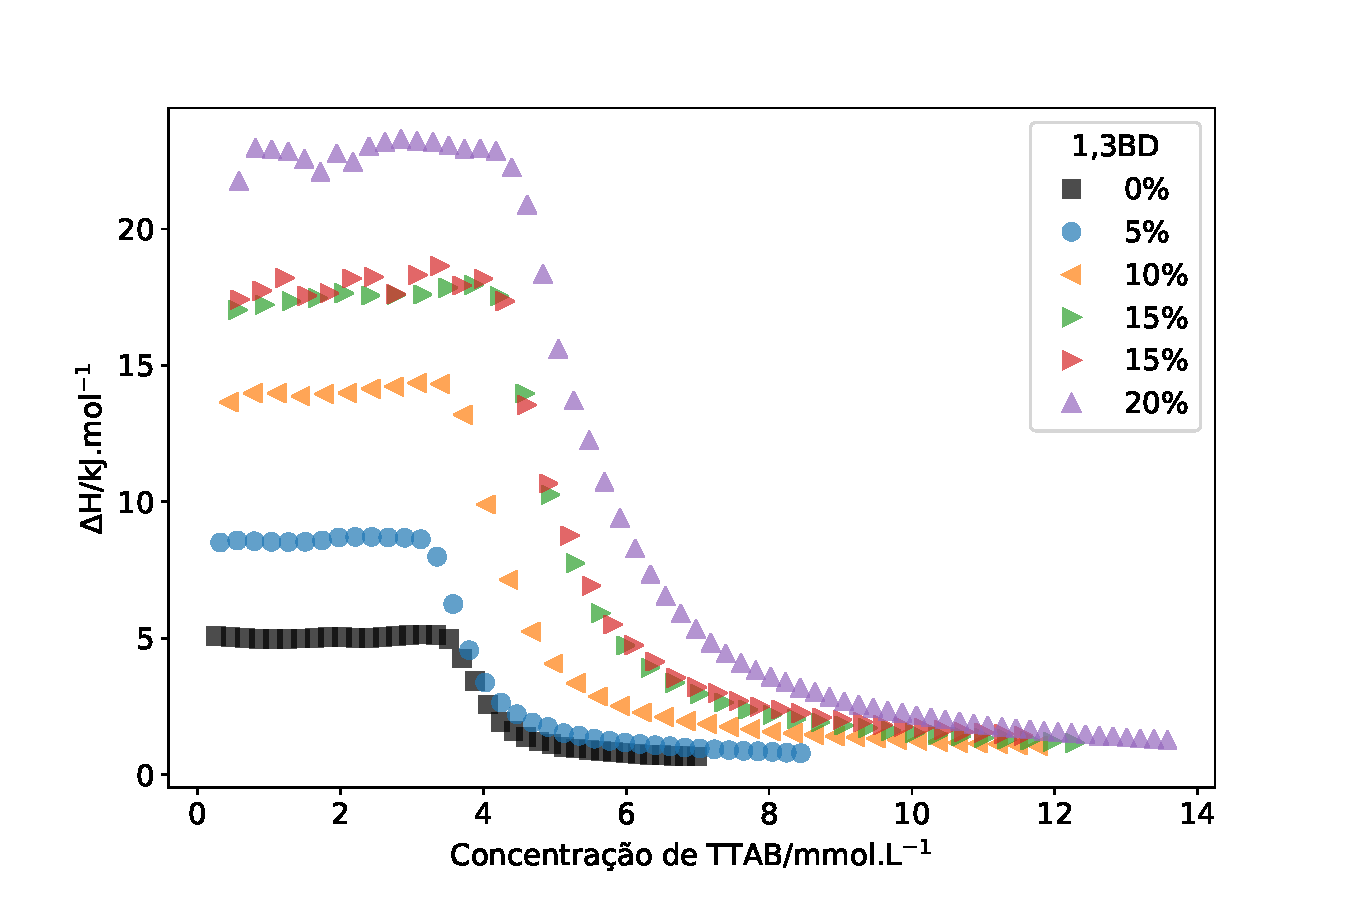
\includegraphics[width=0.7\textwidth]{imagens/itc/ITC_13BD}
				\caption{Efeito de 1,3-butanodiol na titulação de \TTAB}
				\label{fig:itc_13bd}
			\end{figure}  \index{resultados!1,3-butanodiol}
		
			\begin{figure}[h]
				\centering
				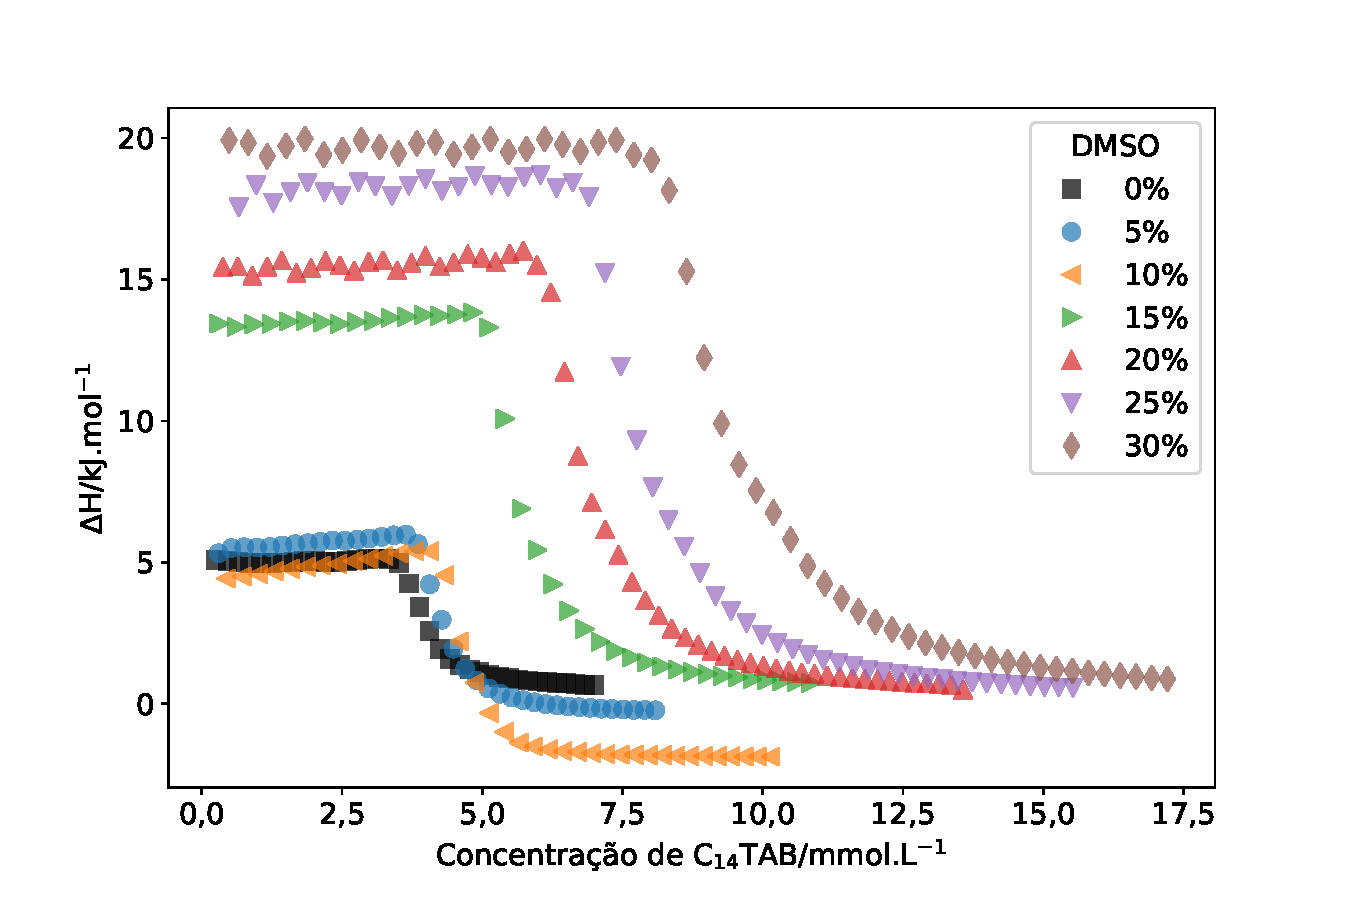
\includegraphics[width=0.7\textwidth]{imagens/itc/ITC_dmso}
				\caption{Efeito de dimetilsulfóxido na titulação de \TTAB.}
				\label{fig:itc_dmso}
			\end{figure} \index{resultados!dimetilsulfóxido}
			
			\begin{figure}[h]
				\centering
				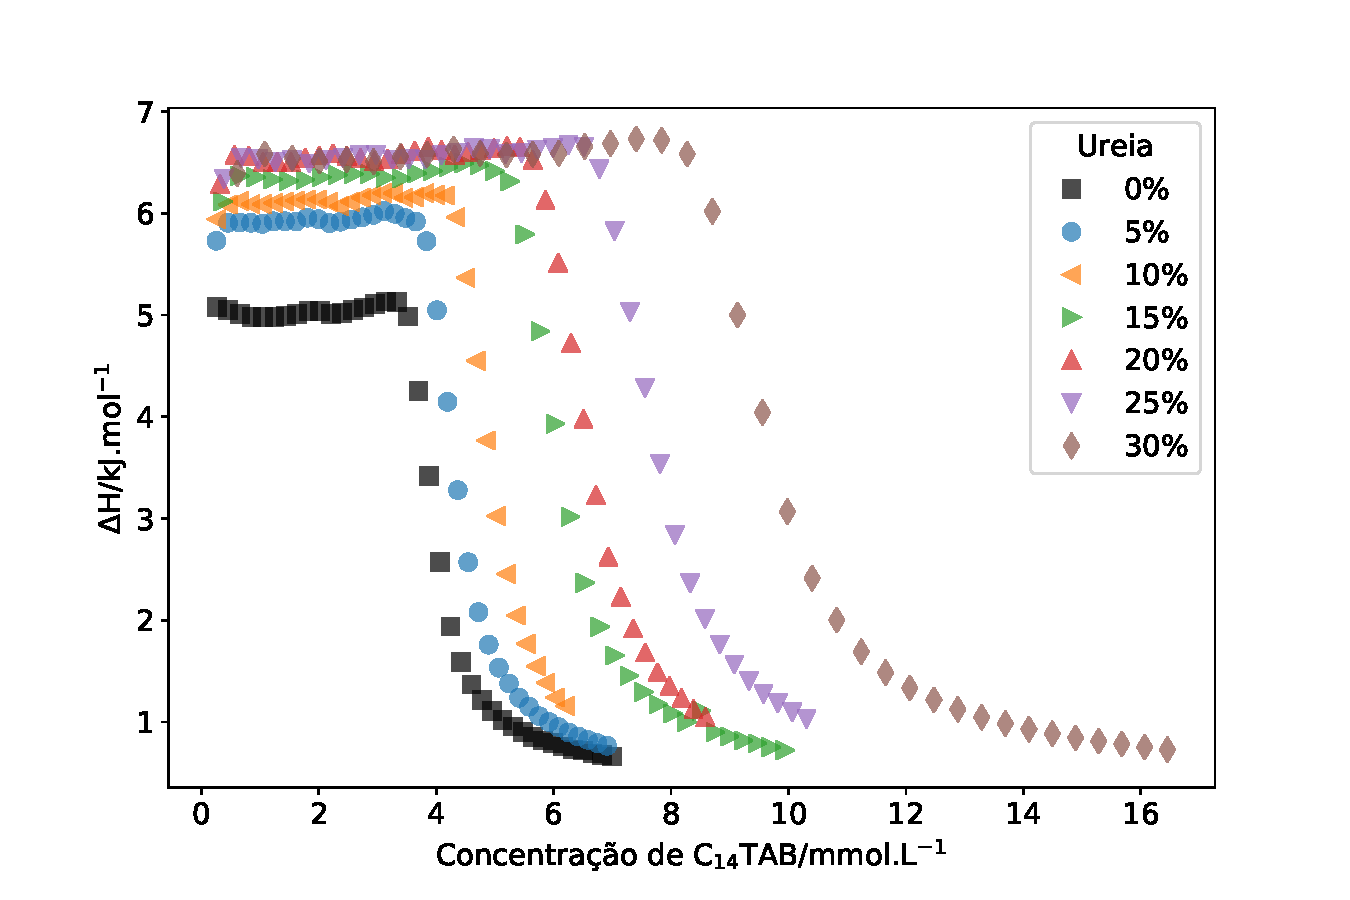
\includegraphics[width=0.7\textwidth]{imagens/itc/ITC_ur}
				\caption{Efeito de ureia na titulação de \TTAB.}
				\label{fig:itc_ureia}
			\end{figure} \index{resultados!ureia}
		
		Novamente, o \BD{} e DMSO mostraram possuir comportamentos semelhantes entre si, portanto o mecanismo que influencia ambas as micelas gigantes quanto esféricas deve ser semelhante. O aumento na \cmc{} já foi observado anteriormente, tanto para o DMSO\cite{Bakshi1993a} quando para \BD.\cite{Abdel-Rahem2012}. A ureia influencia aumentando a \cmc{}, como esperado,\cite{Dias2002} porém não afeta muito o \DHmic{}. Logo, como não há \Sal{} para ser dessorvido das micelas, não ocorrem grandes variações de \DHmic.
		
		\FloatBarrier
		
		Da mesma maneira que anteriormente, essas informações foram resumidas na \autoref{fig:cmc_dh_por_conc}, onde a \cmc{} e o \DHmic{} foram colocados em função da concentração de aditivo.
		
%		\begin{figure}[h]
%			\begin{subfigure}[t]{0.5\textwidth}
%				\centering
%				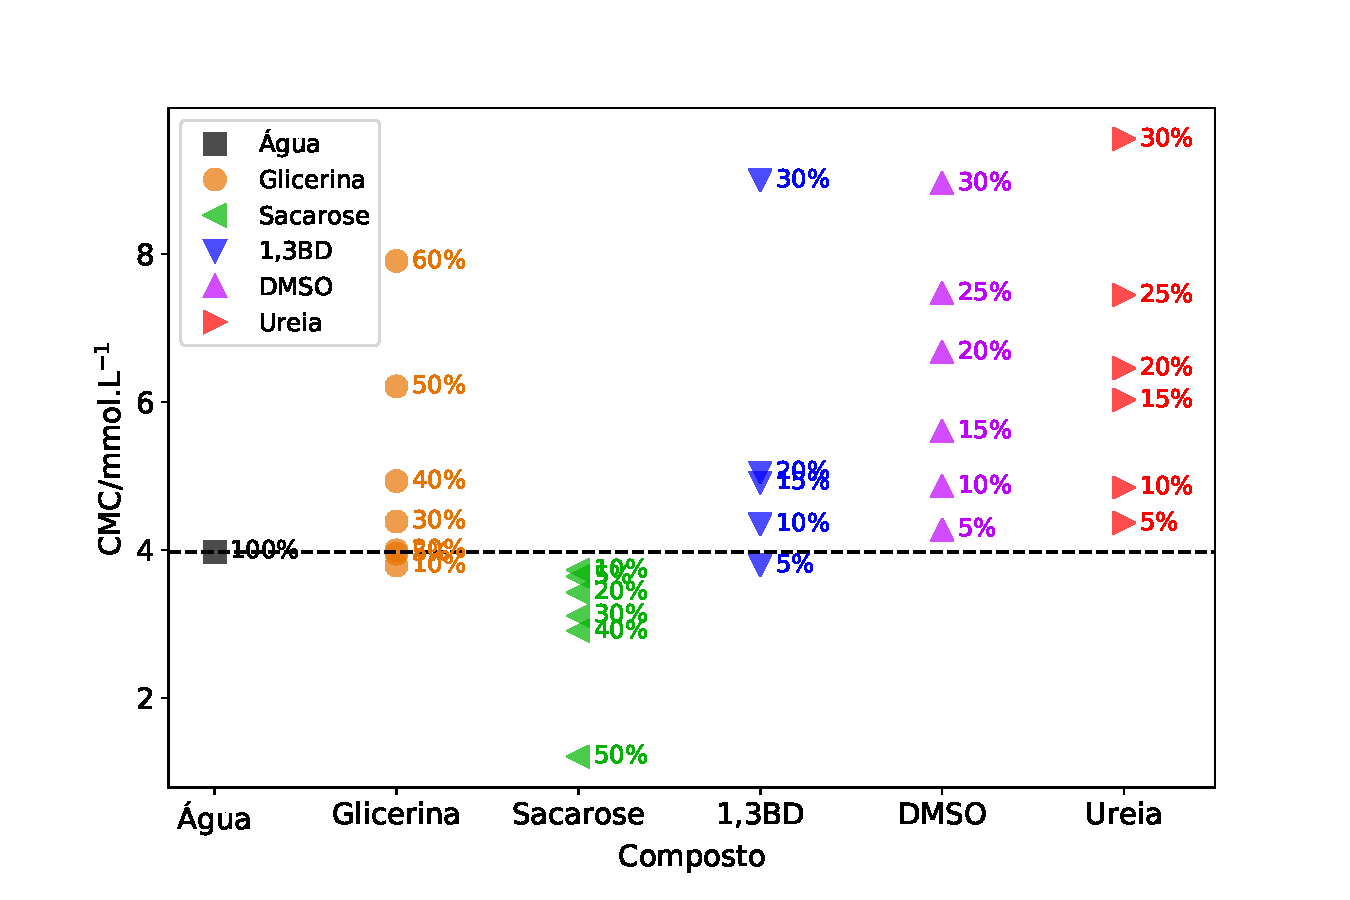
\includegraphics[width=\textwidth]{imagens/itc/CMC_por_composto}
%				\caption{\cmc}
%				\label{fig:cmc_por_composto}
%			\end{subfigure} %
%			\begin{subfigure}[t]{0.5\textwidth}
%				\centering
%				\includegraphics[width=\textwidth]{imagens/itc/DH_por_composto}
%				\caption{\DHmic}
%				\label{fig:dh_por_composto}
%			\end{subfigure}
%		
%			\caption{\cmc{} e \DHmic{} para os vários aditivos}
%			\label{fig:cmc_dh_por_composto}
%		\end{figure}

		\begin{figure}[h]
		%	\centering
			\begin{subfigure}[t]{0.5\textwidth}
				\centering
				\includegraphics[width=\textwidth]{imagens/itc/ITC_cmc_adit}
				\caption{\cmc}
				\label{fig:cmc_por_conc}
			\end{subfigure} %
			\begin{subfigure}[t]{0.5\textwidth}
				\centering
				\includegraphics[width=\textwidth]{imagens/itc/ITC_DH_adit}
				\caption{\DHmic}
				\label{fig:dh_por_conc}
			\end{subfigure}
			
			\caption{\cmc{} e \DHmic{} em função da concentração de aditivo.}
			\label{fig:cmc_dh_por_conc}
		\end{figure}
	
		Vemos que a tendência da \autoref{fig:cmc_por_conc} é bastante similar à \autoref{fig:cwlm_por_conc}, com os aditivos seguindo trajetórias bem comportadas. A tendência relativa dos aditivos também é similar, com a sacarose se mantendo mais próxima à linha basal (neste caso, diminuindo a \cmc), seguido da glicerina e os outros três aditivos se agruparam, mostrando que seus efeitos são similares. Já a \autoref{fig:dh_por_conc} é bastante diferente da \autoref{fig:dhwlm_por_conc}, pois aquele demonstra uma clara tendência, praticamente linear para cada aditivo, exceto em altas concentrações, já este, como visto, não possui tendência clara. Isso mostra que a adição de NaSal aumentou a complexidade do sistema. Correlações mais complexas das propriedades com \cwlm, \cmc, \DHwlm{} e \DHmic{} serão apresentadas na página \pageref{sec:PLS_micelizacao}.
	
%				\begin{figure}[h]
%		\begin{subfigure}[t]{0.5\textwidth}
%			\centering
%			\includegraphics[width=\textwidth]{imagens/itc/Cwlm_por_conc}
%			\caption{\cwlm}
%			\label{fig:cwlm_por_conc}
%		\end{subfigure} %
%		\begin{subfigure}[t]{0.5\textwidth}
%			\centering
%			\includegraphics[width=\textwidth]{imagens/itc/DHwlm_por_conc}
%			\caption{\DHwlm}
%			\label{fig:dhwlm_por_conc}
%		\end{subfigure}
%		
%		\caption{\cwlm{} e \DHwlm{} em função da concentração de aditivo para titulações de \TTAB{} em NaSal 1,5 \mM.}
%		\label{fig:cwlm_dhwlm_por_conc}
%	\end{figure}
	
		\FloatBarrier
		
	\chapter{Parâmetros estudados}
	\label{sec:parametros_estudados}
		
		Existem vários parâmetros físico-químicos que descrevem solventes. Inicialmente, o índice de refração foi escolhido com base nos estudos anteriores de Hoffmann, devido à conexão com a constante de Hamaker (\autoref{eqn:constante_hamaker_lifshitz}), que modula a atração/repulsão coloidal (para duas esferas, vide \autoref{eqn:interacao_duas_esferas}). Quanto mais próximos forem os índices de refração entre o solvente e as micelas gigantes, menor será a atração intermicelar. \index{micelas gigantes!constante de Hamaker} \index{resultados!constante de Hamaker}
		
		A constante dielétrica \(\varepsilon\) é um parâmetro relacionado à polaridade do solvente. Quanto maior for a constante dielétrica, mais fracas são as interações eletrostáticas e dipolares (Equações \ref{eqn:potencial_eletrostático}, \ref{eqn:energia_Keesom}, \ref{eqn:energia_Debye}) pois o campo elétrico oposto gerado pelas moléculas do solvente age no sentido contrário do campo elétrico criado por íons e dipolos. Logo, dois íons de cargas opostas não se atraem com tanta facilidade, já que o campo elétrico de um íon decai muito rapidamente, e as forças entrópicas os afastam. Na constante de Hamaker, a contribuição dipolar, que depende da constante dielétrica, é geralmente pequena, e nunca maior que \(\sfrac{3}{4}kT\), porém pode ser relevante na interação de hidrocarbonetos (núcleo micelar) e água.  \index{micelas gigantes!constante dielétrica} \index{resultados!constante dielétrica}
		
		A permissividade dielétrica e o índice de refração estão ambos relacionados pois dependem da polarizabilidade molecular, e de seu momento de dipolo, \(u\). Efeitos adicionais de separação de carga, que podem ocorrer pela estruturação do solvente em ligações de hidrogênio, não são considerados por essa relação. Logo, é interessante utilizar a constante dielétrica, que considera esses efeitos adicionais do solvente, e o índice de refração, que é proporcional somente à polarizabilidade molecular. É possível combinar a constante dielétrica e o momento de dipolo em um fator, chamado de fator eletrostático, \emph{IT}, mas esses parâmetros não foram considerados neste trabalho devido à presença de misturas de solventes, e pela facilidade de se utilizar propriedades do contínuo na interpretação.\cite{ReichardtSolvents}
		
		Dois parâmetros podem ser utilizados para descrever a estruturação de um solvente, a densidade de energia coesiva \(c\) (\autoref{eqn:densidade_energia_coesiva}), e a pressão interna \(\pi\) (\autoref{eqn:pressao_interna}). \cite{ReichardtSolvents}
		% refs [98-100, 175] do cap 3 do livro de propriedades de solvente
		
		\begin{equation}
			c = \dfrac{\Delta U_V}{V_m} = \dfrac{\Delta H_V - R\cdot T}{V_m}
			\label{eqn:densidade_energia_coesiva}
		\end{equation}
		
		\begin{equation}
			\pi = \left( \dfrac{\partial U}{\partial V_m} \right)_T
			\label{eqn:pressao_interna}
		\end{equation}
		
		\noindent onde \(\Delta U_V\) e \(\Delta H_V\) são a energia interna e entalpia de vaporização e \(V_m\) é o volume molar do líquido. A razão de se utilizar a entalpia/energia interna de vaporização é a seguinte. Ao levar um líquido de seu estado condensado para o estado gasoso, todas as ligações líquido-líquido tiveram que ser rompidas. Logo, dividindo-se essa energia pelo volume molar obtemos uma densidade de energia coesiva.\cite{ReichardtSolvents} 
		
		
		A pressão interna, por sua vez, é a energia necessária para abrir uma cavidade no solvente, pois a variação de volume é necessariamente pequena, de modo a acomodar o soluto. Esse parâmetro é resultado das forças atrativas serem mais fortes que as repulsivas, e portanto está mais relacionado às interações dispersivas e dipolo-dipolo. Já \(c\) está relacionado à interações solvente-solvente específicas, como a ligação de hidrogênio.\cite{ReichardtSolvents}
		
		A diferença entre esses dois parâmetros (\(c - \pi\)) fornece uma medida da força das ligações de hidrogênio, e a razão \(n = \sfrac{\pi}{c}\) fornece uma medida da relação entre a força das ligações de hidrogênio e outras atrações. Essa razão se aproxima de 1 para hidrocarbonetos e é próxima de zero para solventes com fortes ligações de hidrogênio. O quadrado de \(c\) é conhecido também como o parâmetro de solubilidade de Hildebrand, \(\delta\). Esse parâmetro foi estendido para sistemas polares, por Hansen.\cite{ReichardtSolvents}
		
		Porém, os solventes utilizados neste trabalho são todos compostos principalmente por água, e em alguns casos os aditivos são sólidos (ureia, sacarose). Além disso, obter esses parâmetros para as misturas não é uma tarefa para qual o laboratório está equipado. Portanto, é necessário utilizar outro parâmetro que esteja relacionado à estruturação do solvente. Um parâmetro relacionado aos parâmetros de Hildebrand e de Hansen, e que já foi previamente utilizado para discutir sistemas micelares,\cite{Moya2007a, Abdel-Rahem2012} é o parâmetro de Gordon\footnote{Não confundir com o módulo no platô \(G\)} \(G\), definido na \autoref{eqn:Gordon}, que é baseado na tensão superficial, \autoref{eqn:tens_superficial}.\cite{ReichardtSolvents}

		\begin{equation}
			G = \dfrac{\gamma}{\overline{V}_m^{\frac{1}{3}}}
			\label{eqn:Gordon}
		\end{equation}
		
		\begin{equation}
			\overline{V}_m = \overline{V}_{m_{1}}x_1 + \overline{V}_{m_{2}}x_2
			\label{eqn:volume_molar_médio}
		\end{equation}
		
		\noindent onde \(\gamma\) é a tensão superficial do líquido e \(\overline{V}_m\) é o volume molar do líquido que, quando houver mais de um, pode-se utilizar a \autoref{eqn:volume_molar_médio} para calculá-lo. \index{resultados!parâmetro de Gordon}
		
		A razão de se utilizar o parâmetro de Gordon vem de um argumento semelhante ao parâmetro de densidade de energia coesiva. Nesse caso, o aumento da área superficial de um líquido necessita da quebra de interações líquido-líquido das moléculas que vão para a superfície. Um líquido com interações intermoleculares fracas possui uma tensão superficial baixa, pois é fácil quebrar essas ligações. Por outro lado, um líquido com interações intermoleculares fortes, como a água, possui uma tensão superficial bastante alta. Uma grande vantagem de se utilizar o parâmetro de Gordon é que as medidas de tensão superficial de misturas são facilmente realizadas, necessitando então somente a conversão de \(\gamma\) para \(G\). Porém, \citeauthor{ReichardtSolvents} nota que \(c\) é um parâmetro melhor para descrever a energia coesiva.

		\section{Índice de refração} \index{resultados!índice de refração \(n\)}
		
		A \autoref{fig:indice_refracao} mostrou como o índice de refração varia com a concentração de aditivo. Como os resultados reológicos evidenciaram, considerar somente o índice de refração não é uma maneira muito boa para explicar o comportamento reológico. Caso contrário, haveria um padrão notável num gráfico comparativo das concentrações e entalpias. Isso está evidenciado nas Figuras \ref{fig:cwlm_dhwlm_por_n} e \ref{fig:cmc_dh_por_n}, onde não há um padrão geral observado para todos os aditivos.
		
		\begin{figure}[h]
			\begin{subfigure}[t]{0.5\textwidth}
				\centering
				\includegraphics[width=\textwidth]{imagens/itc/Cwlm_por_n}
				\caption{\cwlm}
				\label{fig:cwlm_por_n}
			\end{subfigure} %
			\begin{subfigure}[t]{0.5\textwidth}
				\centering
				\includegraphics[width=\textwidth]{imagens/itc/DHwlm_por_n}
				\caption{\DHwlm}
				\label{fig:dhwlm_por_n}
			\end{subfigure}
			
			\caption{\cwlm{} e \DHwlm{} em função do índice de refração. A reta tracejada indica os resultados para a água pura.}
			\label{fig:cwlm_dhwlm_por_n}
		\end{figure}
		
		\begin{figure}[h]
			\begin{subfigure}[t]{0.5\textwidth}
				\centering
				\includegraphics[width=\textwidth]{imagens/itc/CMC_por_n}
				\caption{\cmc}
				\label{fig:cmc_por_n}
			\end{subfigure} %
			\begin{subfigure}[t]{0.5\textwidth}
				\centering
				\includegraphics[width=\textwidth]{imagens/itc/DH_por_n}
				\caption{\DHmic}
				\label{fig:dh_por_n}
			\end{subfigure}
			
			\caption{\cmc{} e \DHmic{} em função do índice de refração.  A reta tracejada indica os resultados para a água pura.}
			\label{fig:cmc_dh_por_n}
		\end{figure}

		Comparando-se as Figuras \ref{fig:cwlm_dhwlm_por_n} e \ref{fig:cmc_dh_por_n}, pode-se observar que há uma correlação entre as \cmc{} e \cwlm. Aparentemente há um grupo composto de \BD, DMSO e ureia. Glicerina e sacarose desviam-se significativamente, sendo que sacarose possui o comportamento mais diferenciado, não havendo mudança na \cwlm{} e uma diminuição da \cmc{}.
		
		Agrupamentos desse tipo não podem ser feitos com as entalpias, que parecem ter valores bastante variáveis. Porém, é necessário enfatizar que os valores de entalpia obtidos para a formação de micelas gigantes não são tão confiáveis quanto os de formação de micelas esféricas. Para obter os perfis completos de formação de micelas gigantes, foi necessário aumentar a concentração de surfactante na seringa. Isso reduz a precisão na região inicial do perfil, onde é calculado o \DHwlm. Além disso, a resolução dos entalpogramas obtidos pelo calorímetro PEAQ é menor (39 pontos) do que no VP-ITC (90 pontos). Esse problema possui menor relevância para \cwlm{}, que foi definida como sendo o ponto mínimo da curva, não uma subtração de duas regiões pré e pós-micelar.  Apesar disso, o padrão observado para as mudanças de entalpia na presença de ureia podem ser explicadas pelo aumento da constante dielétrica do meio, como previamente mencionado.
	
		É interessante notar que as figuras que comparam as concentrações de formação e entalpias com o índice de refração (Figuras \ref{fig:cwlm_dhwlm_por_conc} e \ref{fig:cwlm_dhwlm_por_n}, \ref{fig:cmc_dh_por_conc} e \ref{fig:cmc_dh_por_n}) e a concentração de aditivo são bastante semelhantes. Isso se deve à dependência praticamente linear em baixas concentrações do índice de refração com a concentração de aditivo na escala mássica, um dos motivos para essa escala ser escolhida.
		
		\FloatBarrier
		
		\section{Constante dielétrica} \index{resultados!constante dielétrica \(\varepsilon\)}
		
		A constante dielétrica está relacionada ao grau de dissociação de espécies iônicas em solução. Quanto maior a constante, maior o grau de dissociação. Isso resulta, por exemplo, no aumento da \cmc{} pois há menos contraíons para reduzir a carga superficial micelar. A contribuição desse parâmetro já havia sido levantada em um estudo anterior.\cite{Abdel-Rahem2012}
		A \autoref{fig:cte_dieletrica} mostra como a constante dielétrica varia em função da concentração de aditivo.
		
		\begin{figure}[h]
			\centering
			\includegraphics[width=0.7\textwidth]{imagens/propriedades/cte_dieletrica}
			\caption{Constante dielétrica em função da concentração de, a 25°C, de sacarose,\cite{Malmberg1950a} DMSO,\cite{Kaatze1989a} \BD,\cite{Piekarski1995} ureia\cite{Wyman1933}, e a 20°C, glicerina.\cite{Akerlof1932}}  % ureia: 25°C. DMSO: 25°C, sacarose: 25°C, Glicerina:20°C, 1,3BD:25°C
			\label{fig:cte_dieletrica}
		\end{figure}
	
		Não há variação entre o comportamento da sacarose e glicerina, e o DMSO praticamente não afeta a constante dielétrica na faixa de concentração estudada. O \BD{} possui sempre os menores valores de \(\varepsilon\), o que indica que nessas soluções há a menor dessorção de contraíons da superfície micelar. O aditivo que afeta a constante dielétrica mais diferentemente dos outros é a ureia, que aumenta \(\varepsilon\). Isso se mostrará crucial para explicar seu comportamento diferenciado.
	
		É possível que, com a dessorção de \Sal{} das micelas, as amostras com maior concentração de ureia se tornem mais carregadas positivamente. Logo, a formação de uma rede ramificada de micelas é menos favorável, pela carga superficial. Por essa razão, não se observa a região intermediária de viscosidade menor, e a viscosidade observada é próxima àquela do sistema altamente carregado.
		
		Os outros aditivos agem de maneira contrária, porém, a quantidade de \Sal{} incorporado já é bastante alta, então a ação de incorporar mais salicilato não tem um efeito tão forte. % todo: achar ref que fala do grau de incorporação de nasal.
		Todavia, ainda é necessário considerar se o aumento da hidrofobicidade do solvente acarretaria numa dessorção de salicilato, apesar de que, devido à sua carga, sua interação com a superfície micelar deve ser mais forte em solventes mais apolares.
	
		Da mesma maneira que o índice de refração, os parâmetros dos ITCs serão comparados com a constante dielétrica do meio para tentar observar algum padrão. Essas comparações estão na \autoref{fig:cwlm_dhwlm_por_eps} e \autoref{fig:cmc_dh_por_eps}.

		
		Algumas observações podem ser feitas quanto aos resultados observados. Aparentemente todos os aditivos possuem uma divergência única do ponto inicial, água, não havendo muita correlação entre eles, com exceção da \DHmic{}, onde a glicerina, sacarose e \BD{} aparentam seguir uma tendência semelhante. A ureia, em todos os casos, diverge pois seu valor de constante dielétrica aumenta. O DMSO não afeta grandemente \(\varepsilon\), mas tanto as concentrações quanto entalpias são fortemente afetadas pelo aumento de sua concentração. Isso indica que a constante dielétrica, por si só, também não consegue explicar os fenômenos observados. Porém, ela é necessária para capturar a divergência observada com a ureia.
		
		\begin{figure}[h]
			\begin{subfigure}[t]{0.5\textwidth}
				\centering
				\includegraphics[width=\textwidth]{imagens/itc/Cwlm_por_eps}
				\caption{\cwlm}
				\label{fig:cwlm_por_eps}
			\end{subfigure} %
			\begin{subfigure}[t]{0.5\textwidth}
				\centering
				\includegraphics[width=\textwidth]{imagens/itc/DHwlm_por_eps}
				\caption{\DHwlm}
				\label{fig:dhwlm_por_eps}
			\end{subfigure}
			
			\caption{\cwlm{} e \DHwlm{} em função da constante dielétrica \(\varepsilon\).}
			\label{fig:cwlm_dhwlm_por_eps}
		\end{figure}
		
		\begin{figure}[h]
			\begin{subfigure}[t]{0.5\textwidth}
				\centering
				\includegraphics[width=\textwidth]{imagens/itc/CMC_por_eps}
				\caption{\cmc}
				\label{fig:cmc_por_eps}
			\end{subfigure} %
			\begin{subfigure}[t]{0.5\textwidth}
				\centering
				\includegraphics[width=\textwidth]{imagens/itc/DH_por_eps}
				\caption{\DHmic}
				\label{fig:dh_por_eps}
			\end{subfigure}
			\caption{\cmc{} e \DHmic{} em função da constante dielétrica \(\varepsilon\) do meio.}
			\label{fig:cmc_dh_por_eps}
		\end{figure}
		
		\FloatBarrier
		
		\section{Coesão do solvente e Parâmetro de Gordon} \index{resultados!coesão do solvente} \index{resultados!parâmetro de Gordon}
		
		Devido à incapacidade dos outros parâmetros explicarem o comportamento reológico e calorimétrico, procuramos por outras propriedades que possam estar relacionadas. Consultando trabalhos anteriores, pensamos na coesão do solvente para explicar o comportamento reológico e calorimétrico. Solventes bastante estruturados, como a água, diminuem a \cmc{} devido ao aumento da penalidade entrópica. Além disso, estipulamos que solventes mais bem estruturados devem dificultar a locomoção das micelas gigantes durante os processos de reptação, aumentando a viscosidade aparente. A partir disso, foram coletadas informações sobre a coesão dos solventes utilizados.
		
		Glicerina na concentração de 43\% (m/m) possui uma probabilidade reduzida de ligações de hidrogênio, portanto a percolação da rede de ligações de hidrogênio é reduzida.\cite{Parsons2001a, Dashnau2006}. Já açúcares são desestruturadores em baixas concentrações e estruturadores em altas. Para a glicose, a estruturação acontece em torno de 25-30\% m/m,\cite{Giangiacomo2006} já outros estudos mencionam 37\% (m/m).\cite{Ueberreiter1982} Sacarose foi descrita em trabalhos anteriores \cite{Song2008a} como aditivo para aumento da separação interlamelar, semelhante à glicerina. É possível que a sacarose afete as micelas e não as bicamadas devido à maior área de contato das micelas com o solvente. Além disso, a reologia observa a dinâmica das micelas ao fluir pelo solvente, já a distância interlamelar é uma propriedade estática, e seria melhor comparada com uma distância intermicelar média.
		
		DMSO foi demonstrado como um agente desestruturador em altas concentrações e estruturador em baixas, e essas propriedades foram descritas como fracas frente à capacidade do DMSO em solubilizar moléculas de surfactante.\cite{Bertoluzza1979b}
		Já o papel da ureia é inconclusivo de acordo com a literatura, com três mecanismos propostos em estudos.\cite{Dias2002}, a saber, um mecanismo direto, um mecanismo indireto, e simplesmente um solvente mais polar. O mecanismo direto estabelece que ligações de hidrogênio favoráveis entre água e ureia contribuem para a troca de moléculas de solvente ao redor de regiões hidrofóbicas, aumentando sua solubilidade. O mecanismo indireto se baseia na desestruturação da água, diminuindo o custo energético/penalidade entrópica para solubilizar grupos apolares. O terceiro mecanismo propõe que a ureia aumenta a estabilidade de íons livres e grupos polares em solução devido ao aumento da constante dielétrica do meio.\cite{Dias2002}
		
		Para seguir a lógica das discussões na outra seção, é necessário levantar uma propriedade que traduza o conceito de coesão do solvente para um número mensurável. O parâmetro de Gordon já foi utilizado na literatura com esse propósito, então ele será utilizado neste trabalho.\cite{Moya2007a, Abdel-Rahem2012} Não foi utilizado o parâmetro de densidade de energia coesiva \(c\) devido à dificuldade de medir esse parâmetro. Porém, é necessário reforçar que \(G\) não traduz perfeitamente o conceito de estruturação, e será utilizado mais como uma maneira para facilitar a discussão. O parâmetro de Gordon já foi definido na \autoref{eqn:Gordon}.
		
		As tensões obtidas estão na \autoref{fig:tensao_superficial_por_conc} e os valores do parâmetro de Gordon obtidos estão na \autoref{fig:param_gordon_por_conc}. \index{resultados!tensão superficial}
		
		\begin{figure}[h]
			\centering
			\includegraphics[width=0.7\textwidth]{imagens/propriedades/tensao_superficial}
			\caption{Tensão superficial de misturas binárias dos aditivos em água}
			\label{fig:tensao_superficial_por_conc}
		\end{figure}
		
		\begin{figure}[h]
			\centering
			\includegraphics[width=0.7\textwidth]{imagens/propriedades/param_gordon}
			\caption{Parâmetro de Gordon das misturas binárias dos aditivos em água}
			\label{fig:param_gordon_por_conc}
		\end{figure}
		
		Podemos observar que os dois gráficos possuem basicamente o mesmo formato. A maior alteração ocorre devido à divisão pelo volume molar, onde a alta massa da sacarose mascara o aumento de sua tensão superficial, tornando os valores de \(G\) constantes. Essa divisão também diferencia as curvas de ureia e sacarose. \label{sec:correlacao_G_reologia}
		
		Pelo posição relativa das retas observadas para cada aditivo, podemos construir a seguinte correlação de estruturação do solvente:
		
		\begin{equation*}
			\textrm{1,3-BD} < \textrm{DMSO} < \textrm{Glicerina} < \textrm{Ureia} < \textrm{Sacarose}
		\end{equation*}
		
		Essa sequência possui grande correlação com o comportamento reológico (com exceção da ureia). \BD, que possui a menor estruturação, reduz mais fortemente a viscosidade das micelas. Já a sacarose praticamente não afetou a estruturação do solvente, e também não afetou muito a viscosidade. Como mencionado, a ureia é uma exceção devido à grande alteração na constante dielétrica, que deve dessorver moléculas de salicilato das micelas e aumentar sua carga. Isso faz com que o mecanismo principal de relaxação seja a reptação na faixa de concentração estudada, então a viscosidade é sempre alta.
		
		Um mecanismo possível para esse acontecimento é o seguinte. A rede criada pelo solvente é enfraquecida quando a estruturação do solvente (parâmetro de Gordon) está baixa, como está esboçado na \autoref{fig:estrutura_agua_G}. Logo, a movimentação das cadeias das micelas é favorecida, o mecanismo de reptação é acelerado, e então a viscosidade é mais baixa.
		
		\begin{figure}[h]
			\centering
			\includegraphics[width=0.5\textwidth]{imagens/Estrutura_agua_G}
			\caption{Ilustração do efeito do parâmetro de Gordon na estruturação do solvente}
			\label{fig:estrutura_agua_G}
		\end{figure}
		
		\FloatBarrier
		
		Para compreender o efeito do parâmetro de Gordon nas titulações, foram criadas figuras comparativas, da mesma maneira que nas seções anteriores. Os comparativos para a formação de micelas gigantes e micelas esféricas estão nas Figuras \ref{fig:cwlm_dhwlm_por_g} e \ref{fig:cmc_dh_por_g}, respectivamente.
		
		\begin{figure}[h]
			\begin{subfigure}[t]{0.5\textwidth}
				\centering
				\includegraphics[width=\linewidth]{imagens/itc/Cwlm_por_G}
				\caption{\cwlm}
				\label{fig:cwlm_por_g}
			\end{subfigure} %
			\begin{subfigure}[t]{0.5\textwidth}
				\centering
				\includegraphics[width=\textwidth]{imagens/itc/DHwlm_por_G}
				\caption{\DHwlm}
				\label{fig:dhwlm_por_g}
			\end{subfigure}
			\caption{\cwlm{} e \DHwlm{} em função do parâmetro de Gordon}
			\label{fig:cwlm_dhwlm_por_g}
		\end{figure}
		
		\begin{figure}[h]
			\begin{subfigure}[t]{0.5\textwidth}
				\centering
				\includegraphics[width=\textwidth]{imagens/itc/CMC_por_G}
				\caption{\cmc}
				\label{fig:cmc_por_g}
			\end{subfigure} %
			\begin{subfigure}[t]{0.5\textwidth}
				\centering
				\includegraphics[width=\linewidth]{imagens/itc/DH_por_G}
				\caption{\DHmic}
				\label{fig:dh_por_g}
			\end{subfigure}
			\caption{\cmc{} e \DHmic{} em função do parâmetro de Gordon}
			\label{fig:cmc_dh_por_g}
		\end{figure}
		
		Pela inclinação das retas observadas nas Figuras \ref{fig:cwlm_por_g} e \ref{fig:cmc_por_g}, podemos observar o quão forte é o efeito de uma mudança no parâmetro de Gordon do aditivo específico na concentração de micelização. A ureia possui o efeito mais forte, onde uma pequena variação de \(G\) aumentou muito a \cmc e \cwlm, porém isso se deve principalmente ao aumento de \(\varepsilon\). Sacarose não afetou a \cwlm{} e diminuiu a \cmc, pelas razões já discutidas. Os outros três aditivos seguem uma tendência semelhante, onde uma diminuição de \(G\) resulta no aumento gradativo de \cwlm{} e \cmc. Pela inclinação, \BD{} possui o efeito mais brando na \cwlm, mas se a concentração de aditivo for levada em consideração também, vemos que seu efeito é bastante significativo, atingindo a \cwlm{} de 4 \mM{} com 25\% de aditivo, comparado com glicerina, que atingiu essa concentração com 60\%. Interessantemente, até 20\%, o efeito do \BD{} na \cmc{} é bastante pequeno, menor que o DMSO, e há um salto em 30\%, equiparando-se ao DMSO.
				
		As \DHwlm{} não possuem uma ordenação clara. Ureia aparenta ter comportamentos divergentes entre soluções de concentrações baixas (\(<\) 15\%) e altas (\(\ge\) 15\%). Já a \DHmic{} possui padrões, como os valores de ureia agrupados, pois não há salicilato para ser dessorvido. Glicerina e DMSO novamente possuem um comportamento relativamente próximo, e \BD{} tem o menor efeito na entalpia por variação de \(G\). A sacarose diminui a \DHmic{} e a \cmc{}, apesar de não afetar \(G\), indicando que seu papel está relacionado com a interação com as micelas, não somente seu efeito no solvente.
		
		A correlação do parâmetro de Gordon é especialmente forte com o comportamento reológico (página \pageref{sec:correlacao_G_reologia}), e, como será visto há algumas correlações que podem ser feitas com a calorimetria. Deve ser enfatizado que esse parâmetro, por si só, também não explica o comportamento completo. É necessário combinar todas essas considerações para entender o sistema. Por exemplo, se um aditivo for ativo na superfície, os valores de tensão superficial irão decair muito fortemente, mas não necessariamente haverá uma alteração forte na estruturação do solvente. Logo, é necessário utilizar aditivos pouco ativos em superfície, e hidrofílicos, caso seja necessário estender este estudo.
		\FloatBarrier
		
		\section{Interação dos aditivos com a superfície micelar}
		
		Uma propriedade importante que deve receber enfoque é a interação dos aditivos com a superfície micelar. Aditivos que interagem fortemente afetam muito os processos de autoassociação, como demonstra o salicilato de sódio. Efeitos semelhantes, mas menos intensos, podem complementar os parâmetros levantados até o momento.
		
		Estudos da influência de álcoois lineares na viscosidade de micelas gigantes de C\textsubscript{16}TASal e CPySal\cite{Bayer1986} mostraram que quando álcoois de cadeia curta interagiam com a superfície micelar, agem como um cossolvente e diminuem o comprimento das micelas, logo diminuindo sua viscosidade. Caso \BD{} se comporte de maneira similar, esse é mais um efeito que pode resultar nas quedas fortes da viscosidade. Um estudo mostra que o \BD{} interage como cosurfactante em cristais líquidos, o que reforça a teoria de seu efeito em micelas gigantes.\cite{Iwanaga1998a} A reologia oscilatória (\autoref{sec:reologia_oscilatoria}) mostra que o módulo no platô \(G\) para as soluções com \BD{} é menor que nos outros aditivos, reforçando a ideia de que houve uma alteração na estrutura das micelas. DMSO aparentemente se localiza na superfície micelar, logo abaixo da cabeça dos surfactantes, e altera a flexibilidade de lamelas,\cite{Notman2006} portanto é possível que o mesmo ocorra com as micelas gigantes, o DMSO iria aumentar a flexibilidade. A interação entre \Sal{} e DMSO na superfície merece mais estudos.
		
		A presença desses aditivos na superfície das micelas durante a relaxação também pode afetar a hidrofilicidade das mesmas, afetando o mecanismo de ``sticky contacts''. Isso levaria a uma diminuição na viscosidade das micelas. O \BD{} poderia se localizar na superfície micelar, aumentando sua hidrofilicidade, em comparação com as metilas do grupo trimetilamônio, levando à uma diminuição na viscosidade. A glicerina, por ser mais polar, possivelmente não se concentraria tanto na mesma região que \BD, logo seria menos eficaz em diminuir a viscosidade ou aumentar a \cmc. A posição das hidroxilas do \BD{} permite que seus grupos polares sejam expostos para uma mesma direção, já a glicerina, devido à repulsão entre as três hidroxilas próximas, não permite que todas se alinhem no mesmo plano, dificultando sua inclusão na superfície micelar.0  O DMSO pode se solubilizar na superfície micelar e interagir com os grupos metila, pois é menos polar que os outros aditivos, e isso pode resultar em uma diminuição maior na viscosidade que a glicerina, mas não tanto quanto o \BD{}. 
		
		A sacarose diminui a \cmc{} de outros surfactantes, como SDS, \CTAB{} e Brij 35, pela interação de suas hidroxilas com a superfície micelar reduzindo a repulsão, e pela estruturação do solvente. Logo, a diminuição de \(n\) e \(\varepsilon\), que deveriam aumentar a \cwlm{}, são compensadas e a \cwlm{} é mantida. Não há uma diminuição de \cwlm, como houve de \cmc, pois o salicilato interage mais fortemente com a superfície micelar, deslocando as hidroxilas da sacarose, logo seu efeito é principalmente na estruturação do solvente.
		
		\section{Correlações simultâneas dos parâmetros com \cmc{} e \DHmic}
		\label{sec:correlacao_params_cmc_dh}
		
		Até este momento, foram feitas correlações dos parâmetros do solvente com as propriedades calorimétricas mensuradas somente um a um, com raros casos explicados considerando-se outros parâmetros simultaneamente. Seria interessante tentar correlacionar todas essas propriedades simultaneamente, ou seja, realizar uma análise multivariada. Na literatura, existem estudos que tentam utilizar análise de fatores e regressões para classificar e estudar as propriedades de solventes na química orgânica\cite{Bohle1977,Chastrette1982, ReichardtSolvents} e também na área coloidal \cite{Moya2007a}. Esses tipos de análise, chamados de regressão linear múltipla, ou ordinária (\emph{OLS}), regressão de componentes principais \emph{PLS} e regressão dos mínimos quadrados parciais \emph{PLS} são principalmente utilizados na área da química analítica, chamada de Quimiometria.\cite{MarciaQuimiometria}
		
		Uma das necessidades para esse tipo de análise é que as variáveis sejam verdadeiramente independentes umas das outras, aditivas e relevantes ao problema em questão. Como pode ser visto pela \autoref{eqn:permissividade_e_indice_refrac}, há certa colinearidade entre o índice de refração e a constante dielétrica. O que as diferencia é fundamentalmente o efeito do solvente e suas interações.
		
		Estudos de classificação dos solventes utilizam os parâmetros já mencionados, e vários outros, como pontos de ebulição, coeficientes de partição, volume molar, constante dielétrica, índice de refração, energia de HOMO e LUMO, parâmetro \(E_T(30)\) obtidos a partir de uma sonda solvatocrômica, parâmetro de Hildebrand e momento de dipolo. Não necessariamente esses parâmetros são independentes, o que resultaria numa redução da dimensão dos dados.\cite{ReichardtSolvents}
		
		O objetivo desta seção é facilitar a interpretação dos resultados calorimétricos através dos parâmetros da solução escolhidos (\(n\), \(\varepsilon\), \(G\)), e não realizar uma descrição quimiométrica completa, nem atribuir muitos significados físicos aos coeficientes encontrados. Não serão mostrados os resultados desses ajustes para reologia (utilizando a viscosidade como variável dependente, os parâmetros e concentração de NaSal como variável dependente) e calorimetria de micelas gigantes (utilizando \cwlm{} e \DHwlm{} como variáveis dependentes e os parâmetros como variáveis dependentes) pois não foram observadas boas correlações.
		
		Inicialmente, será utilizado um método quimiométrico bastante empregado, o PLS (\emph{Partial Least Squares}), depois será utilizado um método de regressão linear múltipla, mais simples, e por último as misturas binárias serão organizadas em grupos de acordo com suas similaridades, através de um dendrograma.
		
		\subsection{PLS} \index{partial least squares@\textsl{partial least squares}}
		
		Aqui será dada uma breve descrição do método de PLS (\emph{Partial Least Squares}). Mais informações podem ser encontradas no excelente livro de \citeauthor{MarciaQuimiometria}. O PLS é baseado no método de PCR (\emph{Principal Component Regression}). No PCR, uma matriz com as informações da amostra, \textbf{X}, é decomposta em duas matrizes, uma denominada escores, \textbf{T}\textsubscript{A}, e outra matriz de pesos, \textbf{L}\textsubscript{A}, e uma matriz de resíduos \textbf{E},
		
		\begin{equation}
			\mathbf{X} = \mathbf{T}_A \mathbf{L}_A^T + \mathbf{E}
			\label{eqn:decomp_PCR}
		\end{equation}
		
		A partir da matriz de pesos, que contém a informação dos componentes principais, realiza-se um ajuste de \cite{MarciaQuimiometria}
		
		\begin{equation}
			\mathbf{y} = \mathbf{T}_A\mathbf{q} + \mathbf{e}
			\label{eqn:modelo_PCR}
		\end{equation}
		
		\noindent onde \textbf{y} é a matriz com as variáveis dependentes que se pretende ajustar, \textbf{q} é o vetor de regressão, que contém os pesos de cada componente principal para realizar o ajuste, e \textbf{e} é uma matriz de resíduos. Outra maneira de se representar essa equação é por uma maneira estendida
		
		\begin{equation}
			\mathbf{y} = q_1\mathbf{t}_1 + \cdots + q_A\mathbf{t}_A + \mathbf{e}_y
			\label{eqn:modelo_PCR_estendido}
		\end{equation}
		
		O vetor de regressão \textbf{q} pode ser estimado pelo método dos mínimos quadrados, o que resulta em
		
		\begin{equation}
			\hat{\textbf{q}} = \left(  \mathbf{T}_A^T \mathbf{T}_A  \right)^{-1}\mathbf{y}
			\label{eqn:estimativa_regress_q}
		\end{equation}

		A matriz de dados nesse caso sofre uma decomposição de valores singulares (\emph{singular value decomposition}, SVD). Porém, para a análise de PLS, uma restrição é imposta durante a decomposição da matriz de dados. Ocorre um compromisso entre a explicação da variância em \textbf{X} e a previsão da variável independente \textbf{y}, então um pouco da propriedade de interesse é colocada no cálculo das variáveis latentes. O algoritmo utilizado para isso neste trabalho foi o algoritmo de NIPALS, proposto por Wold.
		
		% todo: pensar se eu ponho as eqs 74, 80 do livro da Márcia aqui.
		Foram feitas análises de PLS  com o índice de refração, constante dielétrica e parâmetro de Gordon para tentar prever a \cmc{} e a \DHmic. Utilizou-se dois componentes (de 3) em ambos os casos, os dados foram autoescalados de modo a garantir que todas as parâmetros tenham o mesmo peso no modelo final. Logo, os valores de constante dielétrica, na faixa de 50-80, não teriam um peso 50 vezes maior do que os valores de índice de refração, que estão entre 1 e 1,5. 
		
		Utilizou-se validação cruzada com 1 elemento, e sem validação cruzada, e o vetor de previsão permaneceu igual. Essas análises foram realizadas com o software Pirouette 3.11, e comparadas com uma análise que foi feita utilizando pacote \emph{sklearn}, em Python. Esse pacote é livre, ao contrário do Pirouette, então qualquer um pode reproduzir essas análises. Os resultados foram absolutamente iguais, então não serão mostradas as figuras resultantes de ambos os métodos, somente daqueles obtidos no Pirouette. As retas de \cmc{} e \DHmic{} medidos por \cmc{} e \DHmic{} observados estão presentes nas Figuras \ref{fig:pls_cmc_pirouette} e \ref{fig:pls_dh_pirouette}, respectivamente.
		
		\begin{figure}[h]
			\centering
			\includegraphics[width=0.7\textwidth]{imagens/itc/PLS_cmc_pirouette}
			\caption{Comportamento do modelo de \cmc{} criado por PLS, mostrando a correlação entre os valores observados e previstos. A reta preta tracejada mostra o modelo perfeito, onde há uma relação 1:1 entre o observado e o previsto. A reta vermelha mostra o modelo criado, junto com a qualidade do ajuste.}
			\label{fig:pls_cmc_pirouette}
		\end{figure}
	
		\begin{figure}[h]
			\centering
			\includegraphics[width=0.7\textwidth]{imagens/itc/PLS_dh_pirouette}
			\caption{Comportamento do modelo de \DHmic{} criado por PLS, mostrando a correlação entre os valores observados e previstos. A reta preta tracejada mostra o modelo perfeito, onde há uma relação 1:1 entre o observado e o previsto. A reta vermelha mostra o modelo criado, junto com a qualidade do ajuste.}
			\label{fig:pls_dh_pirouette}
		\end{figure} 
		
		Pelas curvas de ajuste e do modelo ideal de \cmc, podemos observar que as amostras que mais divergem da região central são aquelas com alta concentração de aditivo, provavelmente porque a divergência entre suas propriedades e de água pura são muito grandes, e o processo de autoassociação é muito alterado. Além disso, observamos que todas as medidas com \BD{} estão distantes da reta 1:1, e as concentrações de 5 a 20 \% m/m estão paralelas. Isso indica que esse aditivo possui um efeito adicional, aparentemente constante nessa faixa de concentração, que resulta em valores de \cmc{} menores do que o esperado, observando somente os parâmetros escolhidos. Possivelmente, isso é consequência da tendência do \BD{} de interagir na superfície micelar, diminuir a repulsão e facilitar a autoassociação. Seria interessante realizar ajustes de \(\Delta G^\circ_\mathrm{mic}\), ao invés de \cmc, como realizaram outros estudos\cite{Abdel-Rahem2012, Moya2007a}, mas seria necessário estimar o grau de ionização das micelas (\autoref{eqn:itc_DeltaG_mic}), o que exigiria mais estudos utilizando condutividade elétrica.
		
		A previsão de \DHmic{} é melhor que de \cmc, e os compostos que mais fogem do modelo são, novamente, as soluções com maior concentração de aditivo. Em especial, temos 50\% de sacarose, 60\% de glicerina e 30\% de \BD{}.
		
		O código para fazer análise de PLS em Python, e uma figura semelhante à \autoref{fig:pls_cmc_pirouette} está na listagem \ref{lst:pls_cmc_python}.
		
		\begin{listing}[h]
			\inputminted{python}{./python/pls_cmc_sklearn.py}
			\caption{Código utilizado para gerar a dependência de \cmc{} com os parâmetros estudados, resultando na \autoref{fig:pls_cmc_pirouette}. A tabela de dados utilizada possui em cada linha as misturas utilizadas, suas concentrações em \% m/m, as variáveis dependentes (\cmc{} e \DHmic) e as variáveis independentes (\(n\), \(\varepsilon\), \(G\))}
			\label{lst:pls_cmc_python}
		\end{listing}
		
		O resultado desse modelo é um conjunto de coeficientes que, quando multiplicados pelos parâmetros escolhidos (\(n\), \(\varepsilon\), \(G\)), resultam nas propriedades (\cmc, \DHmic). Os membros do vetor não possuem unidades pois os dados foram autoescalados, então é necessário desfazer o autoescalamento para obter uma equação que utiliza coeficientes com as unidades utilizadas neste trabalho. As equações \ref{eqn:PLS_cmcs} e \ref{eqn:PLS_dhs} possuem tanto as relações em unidades usuais (a) quanto autoescaladas (b) para a \cmc{} e \DHmic, respectivamente. % (\mM, \(kJ.mol^{-1}\), \(J.mol^{-1/3}.m^{-3}\))
		
		\label{sec:PLS_micelizacao}
		
		\begin{subequations}
			\begin{align}
				\textrm{CMC}               & = -7,206G              + 0,225\varepsilon             + 27,955n            - 31,871  \label{eqn:PLS_cmc}     \\
				\textrm{CMC}_{\textrm{AS}} & = -0,941G_\textrm{AS}  + 0,864\varepsilon_\textrm{AS} + 0,319n_\textrm{AS}           \label{eqn:PLS_cmc_AS}
			\end{align}
			\label{eqn:PLS_cmcs}
		\end{subequations}
		
		\begin{subequations}
			\begin{align}
				\Delta H_\textrm{mic}^0     &= 7,64G              + 0,395\varepsilon             - 119n                + 101  \label{eqn:PLS_dh} \\
				\Delta H_\textrm{mic, AS}^0 &= 0,300G_\textrm{AS} + 0,458\varepsilon_\textrm{AS} - 0,414n_\textrm{AS}         \label{eqn:PLS_dh_AS}
			\end{align}
			\label{eqn:PLS_dhs}
		\end{subequations}
		
		Os coeficientes das equações autoescaladas estão relacionados com o quanto cada parâmetro afeta a propriedade. Em especial, os sinais mostram se um coeficiente aumenta ou diminui a propriedade modelada. Por exemplo, na \autoref{eqn:PLS_cmc_AS}, o parâmetro de Gordon possui um sinal negativo. Isso significa que um aumento de \(G\) resulta numa diminuição de \cmc, o que está de acordo com a interpretação fornecida para \(G\), que é a coesividade do solvente. Solventes mais coesos resultam em penalidades entrópicas maiores, favorecendo a micelização. A constante dielétrica, por outro lado, promove a dissociação de íons da superfície micelar, logo um aumento de \(\varepsilon\) resulta num aumento de \cmc, pois a repulsão entre os surfactantes é maior. O índice de refração, ou melhor, a diferença entre o índice de refração do meio e do surfactante, está relacionado com a atração entre as moléculas de surfactante. Quanto maior for \(n\), mais próximos são os índices de refração, menor é a atração e maior é a \cmc.
		
		A visualização do efeito desses parâmetros na \DHmic{} é menos trivial. Para interpretar esse fenômeno, é necessário entender a origem da entalpia de micelização. % todo: pesquisar e colocar aqui.
		Observamos que somente o índice de refração possui um sinal negativo, logo um aumento de \(n\) resulta numa diminuição de \DHmic{} (tornando-se mais negativo). Por outro lado, \(G\) e \(\varepsilon\) mostram que aumentos em seus valores resultam em uma diminuição na amplitude de \DHmic. 
		
		\vfill
		
		\FloatBarrier
		\subsection{OLS} \index{ordinary least squares@\textsl{ordinary least squares}}
		
		Outra metodologia que pode ser utilizada para realizar essas correlações é a dos mínimos quadrados ordinários (\emph{ordinary least squares}, OLS). Esse método é mais simples do que o PLS, pois não ocorre uma decomposição em componentes principais. Neste caso, o ajuste é feito reduzindo-se os mínimos quadrados de \cite{MarciaQuimiometria}
	
		\begin{equation}
			\mathbf{A} = \mathbf{CB} + \mathbf{E}
			\label{eqn:ols_modelo_matricial}
		\end{equation}
		
		\noindent onde \textbf{A} é a matriz de resposta \(I \times J\), neste caso, ou \cmc{} ou \DHmic, \textbf{B} é uma matriz \(L \times J\) com os coeficientes que fornecem os pesos para as variáveis, \textbf{C} é uma matriz \(I \times L\) com as variáveis independentes e \textbf{E} é uma matriz \(I \times J\) com os erros de cada ponto. \(I\) é o número de amostras estudado, \(L\) é o número de coeficientes esperado e \(J\) é o número de variáveis independentes utilizado. A nomenclatura pode ser comparada à lei de Beer, \(A = (\varepsilon b)c + \mathrm{erro}\).
		
		Para o estudo da \cmc, a \autoref{eqn:ols_modelo_cmc} pode ser reduzida para
		
		\begin{equation}
		\textrm{CMC} = a_G \cdot G + a_\varepsilon \cdot \varepsilon + a_n \cdot n + e
		\label{eqn:ols_modelo_cmc}
		\end{equation}
		
		Esse tipo de ajuste é igual ao ajuste de uma equação linear, porém com mais de uma variável independente, e é mais recomendado quando o número de variáveis independentes é pequeno.\cite{MarciaQuimiometria}
		
		Foram feitos ajustes por mínimos quadrados ordinários tanto para a previsão da \cmc{} quanto a \DHmic. Os resultados dos ajustes estão nas Figuras \ref{fig:ols_cmc_python} e \ref{fig:ols_dh_python}.
		
		\begin{figure}[h]
			\centering
			\includegraphics[width=0.7\textwidth]{imagens/itc/ols_cmc_python}
			\caption{Comportamento do modelo de \cmc{} criado por OLS, mostrando a correlação entre os valores observados e previstos. A reta preta tracejada mostra o modelo perfeito, onde há uma relação 1:1 entre o observado e o previsto. A reta vermelha mostra o modelo criado, junto com a qualidade do ajuste.}
			\label{fig:ols_cmc_python}
		\end{figure}
		
		\begin{figure}[h]
			\centering
			\includegraphics[width=0.7\textwidth]{imagens/itc/ols_dh_python}
			\caption{Comportamento do modelo de \DHmic{} criado por OLS, mostrando a correlação entre os valores observados e previstos. A reta preta tracejada mostra o modelo perfeito, onde há uma relação 1:1 entre o observado e o previsto. A reta vermelha mostra o modelo criado, junto com a qualidade do ajuste.}
			\label{fig:ols_dh_python}
		\end{figure}

		Para realizar as análises e criar a \autoref{fig:ols_cmc_python}, utilizou-se o código na listagem \ref{lst:ols_cmc_python}.
		
		\begin{listing}[h]
			\inputminted{python}{./python/ols_cmc_statsmodels.py}
			\caption{Código utilizado para gerar a dependência de \cmc{} com os parâmetros estudados, resultando na \autoref{fig:ols_cmc_python}. A tabela de dados utilizada possui em cada linha as misturas utilizadas, suas concentrações em \% (m/m), as variáveis dependentes (\cmc{} e \DHmic) e as variáveis independentes (\(n\), \(\varepsilon\), \(G\)).}
			\label{lst:ols_cmc_python}
		\end{listing}
		
		Os modelos obtidos estão nas Equações \ref{eqn:ols_cmcs} e \ref{eqn:ols_dhs}. O pacote fornece os parâmetros autoescalados, e para convertê-los em parâmetros nas unidades tradicionais, é necessário desescalá-los, o que pode ser feito com o código da listagem \ref{lst:ols_cmc_conversao}.
		
		\begin{subequations}
			\begin{align}
			\textrm{CMC}               & = -7{,}073G              + 0{,}239\varepsilon             + 43{,}5n              -54{,}67  \label{eqn:ols_cmc}     \\
			\textrm{CMC}_{\textrm{AS}} & = -0{,}917G_\textrm{AS}  + 0{,}919\varepsilon_\textrm{AS} +0{,}497n_\textrm{AS}          \label{eqn:ols_cmc_AS}
			\end{align}
			\label{eqn:ols_cmcs}
		\end{subequations}
		
		\begin{subequations}
			\begin{align}
			\Delta H_\textrm{mic}^0     & = 6{,}29G              + 0{,}372\varepsilon             - 138n               + 132  \label{eqn:ols_dh} \\
			\Delta H_\textrm{mic, AS}^0 & = 0{,}258G_\textrm{AS} + 0{,}432\varepsilon_\textrm{AS} - 0{,}480n_\textrm{AS}        \label{eqn:ols_dh_AS}
			\end{align}
			\label{eqn:ols_dhs}
		\end{subequations}
		
		\begin{listing}[h]
			\inputminted{python}{./python/ols_cmc_conversão.py}
			\caption{Código utilizado para transformar os parâmetros dos ajustes de autoescalados para valores habituais.}
			\label{lst:ols_cmc_conversao}
		\end{listing}
		
		Ambos os conjuntos de equações são bastante semelhantes, o que mostra que é possível realizar essas correlações tanto com o método mais complexo (PLS) quanto o método mais simples (OLS). Como o número de parâmetros utilizado é pequeno, é recomendado utilizar o método mais simples. % todo: ref livro Márcia
		
		Assim como nas Equações \ref{eqn:PLS_cmcs} e \ref{eqn:PLS_dhs}, os coeficientes dos parâmetros estão relacionados com o quanto cada parâmetro afeta os processos. Os sinais são iguais, logo as interpretações são as mesmas.
		
		Ambos os modelos apresentados possuem validade somente para os mesmos aditivos, nas faixas empregadas. Não há garantia de que esses modelos consigam prever outros aditivos, a não ser que parâmetros adicionais, mais gerais, sejam propostos.
		
		Além disso, os parâmetros escolhidos não são necessariamente independentes, ou seja, não são ortogonais. Isso diminui a qualidade dos modelos criados. Porém, o motivo principal para a criação desses modelos foi tentar interpretar o conjunto de informações simultaneamente, o que é difícil pois o conjunto de dados possui 5 dimensões. Logo, o objetivo desse estudo foi atingido.
		
		Foram feitas correlações dos parâmetros com as propriedades das micelas gigantes, porém os ajustes foram muito ruins. Isso se deve provavelmente à maior complexidade do sistema, devido à presença de NaSal, e não é possível explicar as variações considerando-se somente três parâmetros.
		
		
		\FloatBarrier
		
		\section{Visualização das semelhanças dos solventes} \index{dendrograma}
		
		Uma maneira de visualizar a similaridade das misturas binárias é utilizando um dendrograma. Esse tipo de gráfico é produzido calculando-se a distância entre pontos. Neste caso, cada ponto, representando cada mistura, está em um espaço tridimensional, de coordenadas \(n\), \(\varepsilon\) e \(G\). Inicialmente, calcula-se a distância entre os pontos, e agrupa-se os pontos que forem mais próximos, e repete-se o cálculo de distância, agora entre os grupos. O método de cálculo para a distância entre grupos varia, podendo ser feito, por exemplo, pelo vizinho mais próximo, pelo vizinho mais distante, ou pela média. \cite{MarciaQuimiometria}
		
		Dito isso, foi montado um dendrograma das misturas binárias, que está presente na \autoref{fig:dendrograma}. Do lado esquerdo do gráfico, os solventes estão sendo vistos com grande ``criteriosidade'', onde pequenas diferenças conseguem separá-los. À medida que se anda para a direita, a ``lupa'' se afasta e os solventes começam a se agrupar, até que todos os solventes são vistos como um só. A reta vertical simboliza o ponto onde a semelhança entre as misturas é de 50\%. Nessa região, os solventes podem ser separados em 6 grupos distintos, que foram coloridos.\cite{MarciaQuimiometria}
		
		\begin{figure}[h]
			\centering
			\includegraphics[width=0.7\textwidth]{imagens/propriedades/dendrograma}
			\caption{Dendrograma das propriedades das misturas binárias. A tabela de propriedades utilizada para esse gráfico é a mesma utilizada para os ajustes}
			\label{fig:dendrograma}
		\end{figure}
		
		Podemos observar a clara divisão entre dois grupos maiores. Um deles, acima, contém todas as misturas com alta concentração de aditivo, e todas as misturas de \BD{}. Abaixo, temos todas as misturas de baixa concentração de aditivo, e todas as de ureia. Dentro do grupo da alta concentração, podemos observar que a sacarose se agrupa, assim como a glicerina. Além disso, concentrações altas de glicerina se assemelham à concentrações um pouco menores de DMSO. \BD{} em baixas concentrações é parecido com DMSO em concentrações moderadas, e \BD{} em altas concentrações se isola.
		
		No grupo de baixa concentração, temos que as misturas de 5-10\% dos aditivos estão próximos, e que sacarose e glicerina 5\% são as mais próximas da água. Ureia em baixas concentrações afetou pouco as propriedades da solução, e se assemelha também à esses compostos, mais do que DMSO 5-10\%. As demais concentrações de ureia se assemelham a esse grupo, provavelmente se separando pela constante dielétrica, e se mantendo próximos pelo índice de refração e parâmetro de Gordon.
		
		Para criar esse dendrograma, utilizou-se o código da listagem \ref{lst:dendrograma}.
		
		\begin{listing}[h]
			\inputminted{python}{./python/dendrograma.py}
			\caption{Código utilizado para criar o dendrograma da \autoref{fig:dendrograma}}
			\label{lst:dendrograma}
		\end{listing}
		\FloatBarrier
		
		\section{Estimativas de \(\Delta G^\circ_{\textrm{mic}}\) e \(\Delta S^\circ_{\textrm{mic}}\)} 
		
		Através da \autoref{eqn:itc_DeltaG_mic} e \autoref{eqn:itc_gibbs_para_entropia} é possível calcular a variação energia livre de Gibbs de micelização, e a variação da entropia de micelização. Para esses cálculos, é necessário ter o grau de ionização \(\alpha\) das micelas , que deve variar muito com a composição da solução. A primeira aproximação desta seção será assumir que as micelas estão totalmente ionizadas, mas idealmente o grau de ionização deveria ser calculado através de medidas de condutividade. Além disso, as equações irão assumir que não há interação dos aditivos com as micelas, e essa será a segunda aproximação. Não existe na literatura um formalismo para a formação de micelas gigantes, então não serão calculados \(\Delta G^\circ\) e \(\Delta S^\circ\) para a formação de micelas gigantes. Os cálculos levaram em conta a concentração de aditivo para calcular a fração molar de surfactante na \cmc.
		
		Para comparações, foi criada a \autoref{fig:dg_tds_por_composto} que contém essas grandezas em função da composição dos aditivos. Ao invés de se utilizar \(\Delta S^\circ_{\textrm{mic}}\) nessa comparação, a contribuição entrópica total, \(-T\Delta S^\circ_{\textrm{mic}}\), foi utilizada. Isso permite avaliar melhor as contribuições relativas de cada grandeza, porque a faixa dos valores de \(\Delta S^\circ_{\textrm{mic}}\) é entre +60 J.mol\menosUm{} a -20 J.mol\menosUm, já os valores de \(\Delta H^\circ_{\textrm{mic}}\) estão na faixa de kJ.mol\menosUm. Essa figura também serve como uma tabela visual.
		
		\begin{figure}[h]
			\begin{subfigure}{0.5\textwidth}
				\centering
				\includegraphics[width=\textwidth]{imagens/itc/DG_por_composto}
				\caption{\(\Delta G^\circ_{\textrm{mic}}\)}
				\label{fig:dg_por_composto}
			\end{subfigure}%
			\begin{subfigure}{0.5\textwidth}
				\centering
				\includegraphics[width=\textwidth]{imagens/itc/TDS_por_composto}
				\caption{\(-T\Delta S^\circ_{\textrm{mic}}\)}
				\label{fig:tds_por_composto}
			\end{subfigure}
			\caption{(\ref{fig:dg_por_composto}) Energia livre de Gibbs de micelização e (\ref{fig:tds_por_composto}) contribuição entrópica para a micelização (\(-T\Delta S^\circ_{\textrm{mic}}\)) para os processos de formação de micelas de \TTAB{} em soluções dos diversos solventes binários utilizados. Essas grandezas foram calculadas a partir da \cmc{} e \DHmic. A reta horizontal é utilizada como comparação com a água.}
			\label{fig:dg_tds_por_composto}
		\end{figure}
		
		Como \(\Delta G^\circ_{\textrm{mic}}\) é obtido a partir da \cmc, é esperado que a tendência de comportamento das duas grandezas seja a mesma. De forma geral, quanto maior é a concentração de aditivo, maior é a \cmc{} e menor é a \(\Delta G^\circ_{\textrm{mic}}\). Há deslocamentos das posições de cada ponto devido à contribuição da alta concentração de aditivo no cálculo da fração molar de surfactante, como fica evidente ao se observar o comportamento da sacarose onde, apesar da \cmc{} gradualmente diminuir, os valores de \(\Delta G^\circ_{\textrm{mic}}\) oscilam ao redor do valor em água, para depois cair bruscamente em 50\%.
		
		Para todos os compostos estudados, a contribuição entrópica para a micelização se torna cada vez menor, indicando que o termo entálpico se torna mais relevante para o processo. Enquanto que, em água, o termo entrópico corresponde a aproximadamente \(\frac{4}{5}\) da contribuição total para \(\Delta G^\circ_{\textrm{mic}}\), em sacarose 50\% o termo entrópico age contra a micelização. De fato, esse é o único aditivo que levou a uma inversão no valor de \(-T\Delta S^\circ_{\textrm{mic}}\). Como esse é também o único aditivo que levou à uma diminuição de \(\Delta G^\circ_{\textrm{mic}}\), isso pode significar que a sacarose levou à micelização por sua interação com a superfície micelar, como já foi mencionado.
		
		Já os outros aditivos tiveram aumentos de \(-T\Delta S^\circ_{\textrm{mic}}\) possivelmente porque a penalidade entrópica diminui com a desestruturação do solvente. Outra observação interessante ocorre nas variações de de 50-- 60\% de glicerina e 20--30\% de \BD. Provavelmente, isso se deve à alteração significativa do solvente nessas condições, que tornou a medida em si pouco confiável, como também foi observado nas figuras anteriores. Se a tendência se mantivesse, possivelmente as concentrações mais altas de glicerina e \BD{} teriam valores de \(-T\Delta S^\circ_{\textrm{mic}}\) positivos ou próximos de zero, indicando o ponto onde a contribuição entrópica se tornou irrelevante, e a entalpia domina. Vemos também que a ureia pouco afeta o termo entálpico, mas afeta a \cmc. Porém, esse deve ser o aditivo que mais afeta a carga superficial micelar, então é difícil criar especulações confiáveis.
		
		\section{Conclusão Parcial} \index{conclusões!aditivos}
		
		Nesta parte do trabalho, mostrou-se o efeito de diversos aditivos na reologia e na calorimetria de micelas gigantes. Os experimentos reológicos mostraram como os processos de relaxação de tensão foram afetados pela adição dos aditivos, e por calorimetria observou-se a espontaneidade de formação de micelas gigantes.
		
		Todos os aditivos estudados tiveram efeitos diferentes nas micelas gigantes. Por um lado, sacarose praticamente não afetou tanto a reologia quanto a formação das micelas gigantes, apesar de promover a formação de micelas esféricas. Por outro lado, 1,3-butanodiol diminuiu fortemente a viscosidade das micelas, porém afetou a formação tanto quanto os outros aditivos. Ureia se mostrou o aditivo mais diferente de todos, aumentando a viscosidade da região de equimolaridade e diminuindo nas outras. Glicerina e DMSO tiveram efeitos semelhantes, tanto diminuindo a viscosidade das micelas quanto sua espontaneidade de formação, com DMSO tendo um efeito um pouco mais forte que glicerina.
		
		% todo: por ref
		Para explicar esses fenômenos, considerou-se alguns parâmetros. Primeiramente, o índice de refração, levantado por Hoffmann e Abdel-Rahem, constante dielétrica, levantado por Abdel-Rahem, e parâmetro de Gordon, também considerado por Abdel-Rahem, mas aplicado somente para micelas esféricas. Combinando-se esses parâmetros com efeitos mais qualitativos, como a posição dos aditivos nas micelas, foi possível explicar os fenômenos observados. O parâmetro com maior correspondência com o comportamento reológico foi o parâmetro de Gordon, relacionado à estruturação do solvente. Quanto mais próximo era o parâmetro de Gordon do solvente ao parâmetro da água pura, menos afetado era o diagrama de viscosidade. Isso pode ser consequência da diminuição da energia coesiva imposta pelo meio e, portanto, mais fácil se torna a dissipação da tensão pelas micelas gigantes. A exceção é ureia, pois é o único aditivo que aumenta a constante dielétrica do meio, e então remove espécies carregadas, como \Sal, da superfície micelar, aumentando a quantidade de \Sal{} necessária para atingir a neutralidade de carga. A interação dos aditivos com a superfície micelar deve ser considerada também, pois 1,3-butanodiol pode agir como um cosurfactante de cadeia curta, diminuindo o tempo de relaxação das micelas, diminuindo sua viscosidade.
		
		As calorimetrias de formação de micelas gigantes foram afetadas pelo solvente. Todos os solventes, com exceção de sacarose, aumentaram a concentração de formação de micelas gigantes, \cwlm, por uma combinação dos efeitos levantados. O parâmetro de Gordon diminui a penalidade entrópica do solvente, desfavorecendo agregação. O aumento da constante dielétrica aumenta a dissociação de espécies, aumentando a repulsão, também levando ao desfavorecimento da agregação. O índice de refração está relacionado à atração das moléculas de surfactante, e quanto maior for o índice, menor é a atração e menor é a tendência de formação micelar.
		
		De modo a observar o efeito de todos os parâmetros simultaneamente, foram realizados ajustes para se obter equações empíricas relacionando os parâmetros às propriedades. Foi possível correlacionar somente as concentrações micelares críticas (\cmc) e entalpias de micelização (\DHmic) aos parâmetros escolhidos. Isso ocorreu possivelmente pela maior simplicidade do sistema sem NaSal.
		
		As grandezas \(\Delta G^\circ_{\textrm{mic}}\) e \(\Delta S^\circ_{\textrm{mic}}\) foram estimadas a partir dos dados calorimétricos. Observou-se que as tendências de \(\Delta G^\circ_{\textrm{mic}}\) eram similares às de \cmc, o que é esperado. Já a \(\Delta S^\circ_{\textrm{mic}}\), ajustada para \(-T\Delta S^\circ_{\textrm{mic}}\) mostrou que quanto maior é a concentração de aditivo, menor é a contribuição entrópica para a micelização, e que em altas concentrações de sacarose, a entropia de micelização contribuía na direção oposta à micelização, apesar da \cmc{} diminuir. Isso mostra que a sacarose interage com a superfície micelar, levando à micelização, e também que os outros aditivos devem desestruturar o solvente de modo a diminuir a penalidade entrópica.
		
		Como perspectivas futuras, pode-se estudar outros aditivos para verificar o quanto os parâmetros levantados conseguem explicar outros comportamentos. Além disso, quantificar a concentração de aditivo na superfície micelar, mostrar como esses aditivos interagem com as moléculas de surfactante, com as moléculas de salicilato, e seus efeitos na cinética de quebra e recombinação micelar aprofundariam o entendimento sobre micelas gigantes. Utilizando-se condutivímetros de boa qualidade, seria possível aprofundar os estudos de calorimetria, e obter valores mais confiáveis para \(\Delta G^\circ_{\textrm{mic}}\) e \(\Delta S^\circ_{\textrm{mic}}\), o que ajudaria na discussão sobre a estruturação do solvente, penalidade entrópica e interação dos aditivos com as micelas.
		
		% todo: criar correlações agora utilizando outros parâmetros para índice de refração e cte dielétrica. Utilizar, por exemplo, (\varepsilon_r - 1 )/(2 \varepsilon_r + 1) e refração molar (V_m (n^2 - 1)/(n^2 - 2)) e cte dielétrica x dipolo, energia coesiva (raiz quadrada do param de hildebrand)
		% todo: tentar correlacionar viscosidades utilizando os parâmetros, mais a conc de salicilato como variáveis independentes
		
	\chapter{Reologia oscilatória} \index{resultados!reologia oscilatória}
	\label{sec:reologia_oscilatoria}

		Os aditivos afetam a viscosidade das soluções, como visto na \autoref{sec:efeito_aditivos_hidrofilicos}. Neste capítulo, será estudado o efeito dos aditivos na reologia oscilatória das micelas gigantes, que está relacionada aos processos de relaxação das micelas. Para realizar isso, foram escolhidas algumas concentrações de base, localizadas nos picos de viscosidade e no vale. Essas concentrações são 60, 100 e 260 \mM{} de NaSal. Na ausência de aditivo, também foram analisadas as concentrações de 35, 72, 189 e 365 \mM.
		
		As curvas foram ajustadas pelos modelos de Maxwell (Equações \ref{eqn:Maxwell_G1_def}, \ref{eqn:Maxwell_G2_def}), Oldroyd (Equações \ref{eqn:Maxwell_G1_def}, \ref{eqn:modelo_oldroyd_g2}), Jeffreys (Equações \ref{eqn:modelo_jeffreys_g1}, \ref{eqn:modelo_jeffreys_g2}), um modelo com dois elementos Maxwellianos, que será chamado de Dois-Modos (Equações \ref{eqn:modelo_doismodos_g1}, \ref{eqn:modelo_doismodos_g2}) e pelo recém proposto modelo de García-Saraji (Equações \ref{eqn:garcia_saraji_g1}, \ref{eqn:garcia_saraji_g2}). Dos ajustes, foram obtidos os módulos no platô, \(G\), e os tempos de relaxação \(\tau_\mathrm{rel}\), para cada dupla G' e G''. Além disso, foram calculados os coeficientes de determinação \(R^2\) (\autoref{eqn:R2}), e os coeficientes de determinação ajustado \(R\mathrm{'}^{2}\) (\autoref{eqn:R2lin}).\cite{MarciaQuimiometria} Esse tipo de estudo é utilizado na literatura para se avaliar a qualidade de um modelo.\cite{Garcia2018} Com essas informações, foram criados gráficos de Cole-Cole, onde se analisa G'' em função de G', normalizados por \(G\).
		
		\begin{equation}
			R^2 = 1 - \dfrac{SQ_\mathrm{res}}{SQ_\mathrm{Tcor}}
			\label{eqn:R2}
		\end{equation} \index{coeficiente de determinação \(R^2\)}
		
		\begin{equation}
			R\mathrm{'}^{2} = 1 - \dfrac{MQ_\mathrm{res}}{MQ_\mathrm{Tcor}}
			\label{eqn:R2lin}
		\end{equation} \index{coeficiente de determinação ajustado \(R'^2\)}
		
		\noindent onde \(SQ_\mathrm{res}\) é a soma quadrática dos resíduos, \(SQ_\mathrm{Tcor}\) é a soma quadrática total corrigida, \(MQ_\mathrm{res}\) é a média quadrática dos resíduos e \(MQ_\mathrm{Tcor}\) é a média quadrática total corrigida. Esses termos estão definidos nas Equações \ref{eqn:SQres} --- \ref{eqn:MQTcor}.\cite{MarciaQuimiometria}
		
		\begin{equation}
			SQ_\mathrm{res} = \sum_{i=1}^{I} \left( y_i - \hat{y}_i \right) ^ 2
			\label{eqn:SQres}
		\end{equation}
		
		\begin{equation}
			SQ_\mathrm{Tcor} = \sum_{i=1}^{I} \left(y_i - \overline{y} \right)^2
			\label{eqn:SQTcor}
		\end{equation}
		
		\begin{equation}
			MQ_\mathrm{res} = \dfrac{SQ_\mathrm{res}}{I-p}
			\label{eqn:MQres}
		\end{equation}
		
		\begin{equation}
			MQ_\mathrm{Tcor} = \dfrac{SQ_\mathrm{Tcor}}{I - 1}
			\label{eqn:MQTcor}
		\end{equation}
		
		\noindent onde \(y_i\) é o i-ésimo ponto da curva, \(I\) é o número total de pontos, \(\hat{y}\) é a média dos valores de \(y\) (G' ou G''), \(\hat{y}_i\) é o i-ésimo valor previsto pelo modelo e \(p\) é o número de parâmetros do modelo (p.e. modelo de Maxwell possui \(G\), \(\tau_\mathrm{rel}\), \(p=2\)).
		
		O objetivo desta seção é relacionar os reogramas ao perfil de viscosidade no repouso, e determinar qual é a fonte das variações de viscosidade, e se a estrutura micelar foi afetada. Além disso, serão comparados os modelos de ajuste, e se o melhor modelo varia dependendo da região do diagrama. O coeficiente de determinação será utilizado para determinar a qualidade do ajuste, e será estudado se esse parâmetro é confiável.
		
		\section{Água}
		\label{sec:reologia_oscilatoria_experimental_agua}
		\index{resultados!reologia oscilatória!água}
		Primeiramente, será analisado a reologia oscilatória de amostras com 100 \mM{} de \CTAB{} e concentrações crescentes de NaSal. As concentrações foram escolhidas de forma a amostrar todas as regiões do diagrama de viscosidade no repouso, vide \autoref{fig:rh_agua_oscilatorio}, e mesmo assim realizar medidas com todos os aditivos. Por essa razão, as concentrações dos máximos e mínimos estão um pouco deslocadas. As concentrações utilizadas foram 35, 60, 72, 100, 189, 260 e 360 \mM{} de NaSal. Os resultados da reologia oscilatória desses pontos estão na \autoref{fig:oscilatorio_agua}.

		\begin{figure}[h]
			\centering
			\includegraphics[width=0.7\textwidth]{imagens/reologia/RH_agua_oscilatorio}
			\caption{Perfil de viscosidade para amostras com \CTAB{} 100 \mM{} em concentrações crescentes de NaSal. As retas verdes indicam as concentrações utilizadas em todas as análises. As retas azuis tracejadas indicam as concentrações extras utilizadas na análise da água. As bandas cinzas indicam as cinco regiões desse tipo de diagrama.}
			\label{fig:rh_agua_oscilatorio}
		\end{figure}
		
		\begin{figure}[h]
			\centering
			\includegraphics[width=0.7\textwidth]{imagens/reologia/oscilatorio_agua}
			%\caption[Reogramas para água]{G' (símbolos cheios) e G''(símbolos vazados) em função da frequência de perturbação \(\omega\), em rad.s\menosUm, para amostras com \CTAB{} 100\mM{} e NaSal em concentrações crescentes. Para facilitar a visualização, o ponto de cruzamento para cada curva está indicado por uma reta horizontal. As curvas de 189 e 365\mM{} de NaSal se sobrepuseram.}
			\caption{G' (símbolos cheios) e G''(símbolos vazados) em função da frequência de perturbação \(\omega\), em rad.s\menosUm, para amostras com \CTAB{} 100 \mM{} e NaSal em concentrações crescentes, em água. Para facilitar a visualização, o ponto de cruzamento para cada curva está indicado por uma reta horizontal. As curvas de 189 e 365 \mM{} de NaSal se sobrepuseram.}
			\label{fig:oscilatorio_agua}
		\end{figure}
		
		É possível ver que todas as curvas de G' atingem aproximadamente o mesmo valor em frequências altas, onde se encontra o módulo no platô, \(G\). Além disso, pode-se observar que o ponto de cruzamento, indicativo do inverso tempo de relaxação, também oscila, sendo mínimo em 60 \mM, o máximo de viscosidade, e máximo em 100 \mM, o mínimo de viscosidade. 
		
		Além disso, é possível observar que em frequências altas, os valores de G' e G'', principalmente, começam a oscilar. Essa oscilação não é real, e é devido a limitações de medida do equipamento. Para fazer os ajustes, todos os pontos a partir do momento em que começam a oscilar foram descartados. Os pontos que aparentam não seguir os modelos, mas que não mostram oscilação, foram mantidos. Os ajustes de Maxwell realizados para essas curvas estão nas Figuras \ref{fig:oscilatorio_agua_maxwell1} e \ref{fig:oscilatorio_agua_maxwell2}. O código para esse ajuste se encontra na listagem \ref{lst:ajuste_maxwell}, no fim desta seção. Os outros modelos seguiram o mesmo modelo, variando-se as equações de acordo com o modelo.
				
		\begin{figure}[h]
			\begin{subfigure}[t]{0.5\textwidth}
				\includegraphics[width=\textwidth]{imagens/reologia/oscilatorio_agua_35}
				\caption{[NaSal] = 35 \mM}
				\label{fig:oscilatorio_agua_35}
			\end{subfigure} %
			\begin{subfigure}[t]{0.5\textwidth}
				\centering
				\includegraphics[width=\textwidth]{imagens/reologia/oscilatorio_agua_60}
				\caption{[NaSal] = 60 \mM}
				\label{fig:oscilatorio_agua_60}
			\end{subfigure}
			
			\begin{subfigure}[t]{0.5\textwidth}
				\includegraphics[width=\textwidth]{imagens/reologia/oscilatorio_agua_72}
				\caption{[NaSal] = 72 \mM}
				\label{fig:oscilatorio_agua_72}
			\end{subfigure} %
			\begin{subfigure}[t]{0.5\textwidth}
				\includegraphics[width=\textwidth]{imagens/reologia/oscilatorio_agua_100}
				\caption{[NaSal] = 100 \mM}
				\label{fig:oscilatorio_agua_100}
			\end{subfigure}
		
		\caption{Ajustes de Maxwell para as curvas da \autoref{fig:oscilatorio_agua} de menor concentração de NaSal}
		\label{fig:oscilatorio_agua_maxwell1}
		\end{figure}
	
		\begin{figure}[h]
			\begin{subfigure}[t]{0.5\textwidth}
				\centering
				\includegraphics[width=\textwidth]{imagens/reologia/oscilatorio_agua_189}
				\caption{[NaSal] = 189 \mM}
				\label{fig:oscilatorio_agua_189}
			\end{subfigure} %
			\begin{subfigure}[t]{0.5\textwidth}
				\includegraphics[width=\textwidth]{imagens/reologia/oscilatorio_agua_260}
				\caption{[NaSal] = 260 \mM}
				\label{fig:oscilatorio_agua_260}
			\end{subfigure}
	
		\centering	\begin{subfigure}[t]{0.5\textwidth}
				\includegraphics[width=\textwidth]{imagens/reologia/oscilatorio_agua_365}
				\caption{[NaSal] = 365 \mM}
				\label{fig:oscilatorio_agua_365}
			\end{subfigure} 
		
			\caption{Ajustes de Maxwell para as curvas da \autoref{fig:oscilatorio_agua} de maior concentração de NaSal}
			\label{fig:oscilatorio_agua_maxwell2}
		\end{figure}
	
		Na \autoref{fig:oscilatorio_agua_35}, o ponto de cruzamento visual e o calculado divergem significantemente. Além disso, é observado um aumento de G'' em altas frequências não previsto pelo modelo, e G' também possui uma divergência da planaridade. Isso indica que não há somente um tempo de relaxação nesse sistema, e que outros modos de relaxação se tornam mais evidentes à medida que a frequência aumenta. O mesmo pode ser observado, mas em menor escala, para a \autoref{fig:oscilatorio_agua_60}.
		
		As outras amostras seguiram consideravelmente bem o modelo de Maxwell, com valores de \(R^2\) próximos à unidade, como mostram as caixas de informação. Além disso, observa-se que não há uma diferença significativa entre \(R^2\) e \(R\mathrm{'}^2\). O mesmo ocorreu para os outros modelos, então esse parâmetro não será utilizado.
		
		O mesmo procedimento foi seguido para os outros modelos. Os ajustes não serão mostrados por brevidade. Os resultados dos ajustes se encontram nas Tabelas \ref{tab:g0_agua} --- \ref{tab:R2_agua}.
		
%		\begin{table}[h]
%        \IBGEtab{%
%			\caption{Módulos no platô, \(G_0\) em Pa, em função da concentração de NaSal em \mM, de todos os ajustes}
%			\label{tab:g0_agua}
%		}%
%		{%
%			\begin{tabular}{c | c c c c c}
%				\toprule
%				NaSal & Maxwell             & OldroydB             & Jeffreys             & Dois-Modos 1            & Dois-Modos 2            \\ \midrule
%				 35   & 30,8    \(\pm\) 0,5 & 30,8     \(\pm\) 0,4 & 30,8     \(\pm\) 0,4 & 26,8        \(\pm\) 0,3 & 7,3         \(\pm\) 0,4 \\
%				 60   & 51,5    \(\pm\) 0,3 & 51,5     \(\pm\) 0,3 & 51,5     \(\pm\) 0,3 & 32          \(\pm\) 2   & 21          \(\pm\) 2   \\
%				 72   & 40,0    \(\pm\) 0,1 & 39,9     \(\pm\) 0,1 & 39,9     \(\pm\) 0,1 & 35,9        \(\pm\) 0,9 & 4,6         \(\pm\) 0,9 \\
%				 100  & 52,3    \(\pm\) 0,1 & 52,1     \(\pm\) 0,1 & 52,2     \(\pm\) 0,1 & 3,6         \(\pm\) 0,5 & 49,7        \(\pm\) 0,5 \\
%				 189  & 49,7    \(\pm\) 0,3 & 49,6     \(\pm\) 0,3 & 49,7     \(\pm\) 0,3 & 48,3        \(\pm\) 0,3 & 3,7         \(\pm\) 0,4 \\
%				 260  & 51,6    \(\pm\) 0,3 & 51,5     \(\pm\) 0,3 & 51,5     \(\pm\) 0,3 & 50          \(\pm\) 1   & 3           \(\pm\) 1   \\
%				 365  & 49,8    \(\pm\) 0,2 & 49,6     \(\pm\) 0,2 & 49,7     \(\pm\) 0,2 & 47,0        \(\pm\) 0,3 & 4,2         \(\pm\) 0,3 \\ \bottomrule
%			\end{tabular}
%		}{}
%		\end{table}  


		\begin{table}[h]
	\IBGEtab{%
		\caption{Módulos no platô \(G\), em Pa, em função da concentração de NaSal em \mM, de todos os ajustes}
		\label{tab:g0_agua}
	}%
	{%
		\begin{tabular}{c | c c c c c c}
			\toprule
			NaSal & Maxwell             & OldroydB             & Jeffreys             & Dois-Modos 1            & Dois-Modos 2            & García-Saraji      \\ \midrule
			 35   & 30,8    \(\pm\) 0,5 & 30,8     \(\pm\) 0,4 & 30,8     \(\pm\) 0,4 & 26,8        \(\pm\) 0,3 & 7,3         \(\pm\) 0,4 & 30,9  \(\pm\) 0,4  \\
			 60   & 51,5    \(\pm\) 0,3 & 51,5     \(\pm\) 0,3 & 51,5     \(\pm\) 0,3 & 32          \(\pm\) 2   & 21          \(\pm\) 2   & 51,5  \(\pm\) 0,3  \\
			 72   & 40,0    \(\pm\) 0,1 & 39,9     \(\pm\) 0,1 & 39,9     \(\pm\) 0,1 & 35,9        \(\pm\) 0,9 & 4,6         \(\pm\) 0,9 & 39,9  \(\pm\) 0,1  \\
			 100  & 52,3    \(\pm\) 0,1 & 52,1     \(\pm\) 0,1 & 52,2     \(\pm\) 0,1 & 3,6         \(\pm\) 0,5 & 49,7        \(\pm\) 0,5 & 52,31 \(\pm\) 0,09 \\
			 189  & 49,7    \(\pm\) 0,3 & 49,6     \(\pm\) 0,3 & 49,7     \(\pm\) 0,3 & 48,3        \(\pm\) 0,3 & 3,7         \(\pm\) 0,4 & 49,7  \(\pm\) 0,2  \\
			 260  & 51,6    \(\pm\) 0,3 & 51,5     \(\pm\) 0,3 & 51,5     \(\pm\) 0,3 & 50          \(\pm\) 1   & 3           \(\pm\) 1   & 51,6  \(\pm\) 0,3  \\
			 365  & 49,8    \(\pm\) 0,2 & 49,6     \(\pm\) 0,2 & 49,7     \(\pm\) 0,2 & 47,0        \(\pm\) 0,3 & 4,2         \(\pm\) 0,3 & 49,8  \(\pm\) 0,1  \\ \bottomrule
		\end{tabular}
	}{}
\end{table}   \index{resultados!reologia oscilatória!ajustes}
	
%		\begin{table}[h]
%		\IBGEtab{%
%			\caption{Tempos de relaxação, \(\tau_\mathrm{rel}\) em s, de todos os ajustes, em função da concentração de NaSal em \mM. O segundo tempo de relaxação do modelo de Jeffreys não foi incluído nesta tabela pois todos os valores eram da ordem de 1ms, e possuíam um desvio alto. Esses valores se encontram na tabela \ref{tab:outros_params_agua}.}
%			\label{tab:tr_agua}
%		}%
%		{%
%			\begin{tabular}{c | c c c c c c}
%				\toprule
%				NaSal & Maxwell               & OldroydB               & Jeffreys 1               & Dois Modos 1               & Dois Modos 2               &  \\ \midrule
%				 35   & 24      \(\pm\) 1     & 24       \(\pm\) 1     & 24        \(\pm\) 1     & 29,3        \(\pm\) 0,8   & 0,76        \(\pm\) 0,08  &  \\
%				 60   & 79      \(\pm\) 2     & 79       \(\pm\) 2     & 79        \(\pm\) 2     & 128         \(\pm\) 5     & 38          \(\pm\) 2     &  \\
%				 72   & 4,47    \(\pm\) 0,05  & 4,49     \(\pm\) 0,05  & 4,49      \(\pm\) 0,05  & 4,99        \(\pm\) 0,09  & 1,4         \(\pm\) 0,2   &  \\
%				 100  & 0,209   \(\pm\) 0,001 & 0,212    \(\pm\) 0,001 & 0,212     \(\pm\) 0,001 & 0,055       \(\pm\) 0,008 & 0,221       \(\pm\) 0,002 &  \\
%				 189  & 1,01    \(\pm\) 0,01  & 1,02     \(\pm\) 0,01  & 1,02      \(\pm\) 0,01  & 1,06        \(\pm\) 0,01  & 0,06        \(\pm\) 0,01  &  \\
%				 260  & 2,71    \(\pm\) 0,05  & 2,72     \(\pm\) 0,05  & 2,72      \(\pm\) 0,05  & 2,84        \(\pm\) 0,08  & 0,4         \(\pm\) 0,2   &  \\
%				 365  & 0,90    \(\pm\) 0,01  & 0,911    \(\pm\) 0,008 & 0,911     \(\pm\) 0,008 & 0,971       \(\pm\) 0,007 & 0,15        \(\pm\) 0,02  &  \\ \bottomrule
%			\end{tabular}
%		}{}
%	\end{table}  

		\begin{table}[h]
			\IBGEtab{%
				\caption{Tempos de relaxação, \(\tau_\mathrm{rel}\) em s, de todos os ajustes, em função da concentração de NaSal em \mM. O segundo tempo de relaxação do modelo de Jeffreys não foi incluído nesta tabela pois todos os valores eram da ordem de 1ms, e possuíam um desvio alto. Esses valores se encontram na \autoref{tab:outros_params_agua}.}
				\label{tab:tr_agua}
			}%
			{%
				\begin{tabular}{c | c c c c c c}
					\toprule
					NaSal & Maxwell               & OldroydB               & Jeffreys 1              & Dois Modos 1              & Dois Modos 2              & García-Saraji       \\ \midrule
					 35   & 24      \(\pm\) 1     & 24       \(\pm\) 1     & 24        \(\pm\) 1     & 29,3        \(\pm\) 0,8   & 0,76        \(\pm\) 0,08  & 40    \(\pm\) 8     \\
					 60   & 79      \(\pm\) 2     & 79       \(\pm\) 2     & 79        \(\pm\) 2     & 128         \(\pm\) 5     & 38          \(\pm\) 2     & 110   \(\pm\) 67    \\
					 72   & 4,47    \(\pm\) 0,05  & 4,49     \(\pm\) 0,05  & 4,49      \(\pm\) 0,05  & 4,99        \(\pm\) 0,09  & 1,4         \(\pm\) 0,2   & 4,7   \(\pm\) 0,2   \\
					 100  & 0,209   \(\pm\) 0,001 & 0,212    \(\pm\) 0,001 & 0,212     \(\pm\) 0,001 & 0,055       \(\pm\) 0,008 & 0,221       \(\pm\) 0,002 & 0,219 \(\pm\) 0,004 \\
					 189  & 1,01    \(\pm\) 0,01  & 1,02     \(\pm\) 0,01  & 1,02      \(\pm\) 0,01  & 1,06        \(\pm\) 0,01  & 0,06        \(\pm\) 0,01  & 1,04  \(\pm\) 0,03  \\
					 260  & 2,71    \(\pm\) 0,05  & 2,72     \(\pm\) 0,05  & 2,72      \(\pm\) 0,05  & 2,84        \(\pm\) 0,08  & 0,4         \(\pm\) 0,2   & 2,78  \(\pm\) 0,08  \\
					 365  & 0,90    \(\pm\) 0,01  & 0,911    \(\pm\) 0,008 & 0,911     \(\pm\) 0,008 & 0,971       \(\pm\) 0,007 & 0,15        \(\pm\) 0,02  & 0,95  \(\pm\) 0,02  \\ \bottomrule
				\end{tabular}
			}{}
		\end{table}  

%	\begin{table}[h]
%		\IBGEtab{%
%			\caption{Valores da viscosidade em altas frequências \(\eta_{\infty}\), do modelo de Oldroyd, e do segundo tempo de relaxação do modelo de Jeffreys, em ms.}
%			\label{tab:outros_params_agua}
%		}%
%		{%
%			\begin{tabular}{c | p{3cm} | p{3cm}}
%				\toprule
%				NaSal  &  \(\eta_\infty\)/Pa.s          &  \(\tau_{rel,2}\)/ms            \\ \midrule
%				35    &  0,14            \(\pm\) 0,05  &  5                \(\pm\) 1     \\
%				60    &  0,5             \(\pm\) 0,4   &  10               \(\pm\) 8     \\
%				72    &  0,07            \(\pm\) 0,02  &  1,8              \(\pm\) 0,6   \\
%				100   &  0,023           \(\pm\) 0,004 &  0,45             \(\pm\) 0,08  \\
%				189   &  0,04            \(\pm\) 0,02  &  0,7              \(\pm\) 0,3   \\
%				260   &  0,10            \(\pm\) 0,04  &  2,0              \(\pm\) 0,8   \\
%				365   &  0,07            \(\pm\) 0,01  &  1,4              \(\pm\) 0,3   \\ \bottomrule
%			\end{tabular}
%		}{} 
%	\end{table}  

	\begin{table}[h]
		\IBGEtab{%
			\caption{Valores da viscosidade em altas frequências \(\eta_{\infty}\), do modelo de Oldroyd, do segundo tempo de relaxação do modelo de Jeffreys, em ms, e dos parâmetros \(a\), em s, e b, do modelo de García-Saraji. Esses valores estão próximos aos apresentados pelos autores. \cite{Garcia2018}}
			\label{tab:outros_params_agua}
		}%
		{%
			%\begin{tabular}{c | p{3cm} | p{3cm}}
			\begin{tabular}{c | c c c c}
				\toprule
                NaSal  &  \(\eta_\infty\)/Pa.s          &  \(\tau_{rel,2}\)/ms         & \(a\)/s      &  \(b\) \\ \midrule
				35    &  0,14            \(\pm\) 0,05  &  5                \(\pm\) 1   & 2,8     0,6  &  0,3 0,1 \\
				60    &  0,5             \(\pm\) 0,4   &  10               \(\pm\) 8   & 1,6     0,8  &  0,2 0,4 \\
				72    &  0,07            \(\pm\) 0,02  &  1,8              \(\pm\) 0,6 & 0,2     0,1  &  0,6 0,2 \\
				100   &  0,023           \(\pm\) 0,004 &  0,45             \(\pm\) 0,08& 0,03    0,02 &  0,6 0,2 \\
				189   &  0,04            \(\pm\) 0,02  &  0,7              \(\pm\) 0,3 & 0,05    0,06 &  0,9 0,4 \\
				260   &  0,10            \(\pm\) 0,04  &  2,0              \(\pm\) 0,8 & 0,10    0,09 &  1,0 0,4 \\
				365   &  0,07            \(\pm\) 0,01  &  1,4              \(\pm\) 0,3 & 0,09    0,04 &  0,8 0,2 \\ \bottomrule
			\end{tabular}
		}{} 
	\end{table}  

%	\begin{table}[h]
%		\IBGEtab{%
%			\caption{Valores do coeficiente de determinação \(R^2\) de todos os ajustes. O valor de coeficiente ajustado não será incluso pois não diverge significantemente.}
%			\label{tab:R2_agua}
%		}%
%		{%
%			\begin{tabular}{c |c c c c}
%				\toprule
%				 NaSal  & Maxwell & OldroydB & Jeffreys & Dois-Modos \\ \midrule
%				35  & 0,914   & 0,925    & 0,925    & 0,988      \\
%				60  & 0,976   & 0,977    & 0,977    & 0,998      \\
%				72  & 0,997   & 0,997    & 0,997    & 0,999      \\
%				100 & 0,999   & 1,000    & 1,000    & 1,000      \\
%				189 & 0,996   & 0,997    & 0,997    & 0,999      \\
%				260 & 0,993   & 0,994    & 0,994    & 0,994      \\
%				365 & 0,998   & 0,999    & 0,999    & 1,000      \\ \bottomrule
%			\end{tabular}
%			}{}
%	\end{table}  

	\begin{table}[h]
		\IBGEtab{%
			\caption{Valores do coeficiente de determinação \(R^2\) de todos os ajustes. O valor de coeficiente ajustado não será incluso pois não diverge significantemente.}
			\label{tab:R2_agua}
		}%
		{%
			\begin{tabular}{c |c c c c c}
				\toprule
                 NaSal  & Maxwell & OldroydB & Jeffreys & Dois-Modos & García-Saraji \\ \midrule
				35  & 0,914   & 0,925    & 0,925    & 0,988  & 0.941    \\
				60  & 0,976   & 0,977    & 0,977    & 0,998  & 0.979    \\
				72  & 0,997   & 0,997    & 0,997    & 0,999  & 0.998    \\
				100 & 0,999   & 1,000    & 1,000    & 1,000  & 1.000    \\
				189 & 0,996   & 0,997    & 0,997    & 0,999  & 0.997    \\
				260 & 0,993   & 0,994    & 0,994    & 0,994  & 0.994    \\
				365 & 0,998   & 0,999    & 0,999    & 1,000  & 0.999    \\ \bottomrule
			\end{tabular}
		}{}
	\end{table}  

	Os valores de módulo no platô foram todos próximos em todos os modelos, exceto pelas primeiras concentrações, quando a rede micelar ainda está sendo formada. Isso já foi observado anteriormente\cite{Rehage1991}, e que \(G\) essencialmente não varia entre os dois picos, indicando que a estrutura lamelar se mantém constante.
	
	% todo: Rehage e Hoffmann em 1991 mostraram que não muda muito entre os picos. Transição sol-gel. O módulo é dependente da concentração de partículas ou o número de pontos de crosslinking por unidade de volume. Valor constante de G0 indica que a estrutura micelar não muda em função da força iônica. No mesmo artigo, ele fala que no segundo máximo as micelas ficaram negativas.
	No modelo de Dois-Modos, não há uma restrição para os valores de \(G_{0,1}\) e \(G_{0,2}\), e observa-se que os dois módulos variam entre um valor perto de 50 Pa e outro entre 3-5 Pa, praticamente insignificante. Esse segundo módulo, provavelmente, está auxiliando no ajuste da região final de G'', onde há uma divergência para cima de G' e G''. A amostra com 60 \mM{} de NaSal, porém, mostrou dois valores bastante diferentes de \(G\) quando comparados aos outros mas, se somados, resultam no módulo dos outros modelos, mostrando que os dois elementos do modelo são, de fato, aditivos. Isso ocorreu provavelmente porque há uma região pequena antes do cruzamento, então não foi possível ajustar muito bem a curva por completo. Adquirir pontos antes do cruzamento nesse caso é, experimentalmente, muito difícil, pois exigiria muitas horas para completar uma análise, e a secagem da amostra seria difícil de ser adequadamente prevenida. Os desvios de todos os parâmetros estão semelhantes, e são maiores para as amostras longe da concentração de 100 \mM. Uma exceção é, novamente, o modelo de Dois-Modos, que possui incertezas maiores, possivelmente porque variações nesses parâmetros não resultam em mudanças significativas na qualidade do ajuste, já que utilizar um único parâmetro foi adequado.
	
	Os valores de tempo de relaxação seguem o mesmo perfil de viscosidade, como pode ser visto na \autoref{fig:oscilatorio_agua_tr}. Seus valores também estão todos com valores próximos entre os modelos, com exceção do modelo de Dois Modos e de García-Saraji. No modelo Dois Modos, um dos tempos se aproxima dos tempos dos outros modelos, e o outro tempo é diferente. Com 60 \mM, o mesmo fenômeno ocorreu com os tempos de relaxação, mas neste caso a média dos dois tempos (128 e 38), 83, é parecido com os outros tempos de relaxação. Os tempos de relaxação para as amostras com 35 e 60 \mM{} do modelo de García-Saraji demonstraram grande variabilidade em comparação com os outros modelos, em especial a amostra com 60 \mM. Isso pode se dever à falta de pontos antes do cruzamento, sendo que o modelo necessita do perfil completo de viscosidade para estimar como o tempo de relaxação varia com a frequência. O segundo tempo de relaxação do modelo de Jeffreys, presente na \autoref{tab:outros_params_agua}, possui valores muito baixos e com incerteza alta, mostrando que esse parâmetro não é relevante ao ajuste, e também é diferente do segundo tempo de relaxação do modelo Dois-Modos. A viscosidade em frequências altas, do modelo de Oldroyd, que visa ajustar a região de alta frequência de G'', também não teve um ajuste muito bom, com altas incertezas.
	
	\begin{figure}[h]
		\centering
		\includegraphics[width=0.9\textwidth]{imagens/reologia/oscilatório_agua_tr}
		\caption{Tempos de relaxação, em segundos, calculados pelo ajuste dos quatro modelos estudados. As linhas são guias para os olhos, para mostrar a similaridade com o perfil de viscosidade (\autoref{fig:rh_agua_oscilatorio}).}
		\label{fig:oscilatorio_agua_tr}  
	\end{figure}

	
	O coeficiente de determinação possuiu valores muito altos para as amostras com concentração de NaSal maior que 100 \mM, sendo máximo nesse caso. Para as amostras com 35 e 60, o ajuste foi pior. Além disso, pode-se observar que os modelos mais complexos possuem um ajuste melhor. Isso é esperado, pois com mais parâmetros é possível aproximar mais o modelo ao dado experimental. Porém, essa melhoria pode não possuir significado físico, sendo completamente um resultado matemático. Isso ocorreu mais evidentemente nos modelos de Dois Modos e de García-Saraji, onde os parâmetros, em geral, possuíam incertezas maiores pois acabavam descrevendo as mesmas regiões dos espectros mecânicos. A \autoref{fig:ajuste_gs_tm_35} mostra os ajustes do modelo de Dois-Modos e García-Saraji para a amostra com 35 \mM{} de NaSal, evidenciando que o coeficiente de ajuste melhorado não implicou numa descrição melhor do sistema.
	
%	\begin{figure}[h]
%		\centering
%		\includegraphics[width=0.7\textwidth]{imagens/reologia/ajuste_TM_35}
%		\caption{Ajuste com o modelo de Dois-Modos do reograma completo para a amostra com 100 \mM{} de CTAB e 35 \mM{} de NaSal}
%		\label{fig:ajuste_tm_35}
%	\end{figure}

	\begin{figure}[h]
		\begin{subfigure}{0.5\textwidth}
			\centering
			\includegraphics[width=\textwidth]{imagens/reologia/ajuste_TM_35}
			\caption{Dois-Modos}
			\label{fig:ajuste_tm_35}
		\end{subfigure} %
		\begin{subfigure}{0.5\textwidth}
			\centering
			\includegraphics[width=\textwidth]{imagens/reologia/ajuste_GS_35}
			\caption{García-Saraji}
			\label{fig:ajuste_gs_35}
		\end{subfigure}
		\caption{Ajuste do reograma completo para a amostra com 100 \mM{} de \CTAB{} e 35 \mM{} de NaSal com os modelos de Dois Modos e de García-Saraji}
		\label{fig:ajuste_gs_tm_35}
	\end{figure}
	

	Utilizando os valores de \(G\) calculados pelos modelos, foi construído um diagrama de Cole-Cole, presente na \autoref{fig:colecole_agua}. Utilizou-se o \(G\) do modelo de Maxwell, já que os valores entre modelos não variaram muito. Esse tipo de diagrama possui um formato semicircular caso o conjunto de dados seguir bem o modelo de Maxwell. Essa é uma maneira alternativa de se visualizar o quão bons são os ajustes. É possível criar um diagrama sem normalizar G' e G'' por \(G\), mas isso torna a comparação entre sistemas diferentes mais difícil.

		\begin{figure}[b]
			\centering
			\includegraphics[width=0.7\textwidth]{imagens/reologia/colecole_agua}
			\caption{Diagrama de Cole-Cole com G' e G'' normalizado, para amostras com 100 \mM{} de \CTAB{} e concentrações crescentes de NaSal. A linha tracejada mostra como seria o comportamento ideal, 100\% Maxwelliano. As marcas \texttt{x} indicam o último ponto considerado nos ajustes.}
			\label{fig:colecole_agua}
		\end{figure} \index{resultados!reologia oscilatória!Cole-Cole}

	Com o diagrama de Cole-Cole, é possível observar, graficamente, que as amostras com 35 e 60 \mM{} de NaSal são as que menos se ajustam ao modelo, já as outras são melhores. É possível, a partir de diagramas como esses, estimar outras propriedades das micelas (\autoref{eqn:mesh_contorno_por_reologia}) mas isso necessita de valores confiáveis para altas frequências (à direita no diagrama), o que não ocorreu.
	
	\begin{listing}[h]
		\inputminted{python}{./python/ajuste_maxwell.py}
		\caption{Código utilizado para realizar o ajuste de Maxwell de ambos os conjuntos de dados (G' e G'') simultaneamente.}
		\label{lst:ajuste_maxwell}
	\end{listing}
	
	\FloatBarrier
	
	\section{Aditivos} \index{resultados!reologia oscilatória!aditivos}

	O mesmo processo de análise foi feito com os aditivos. Os reogramas foram divididos em várias imagens para facilitar as comparações. As misturas analisadas e as imagens são: 30 e 60\% (m/m) de Glicerina (\autoref{fig:oscilatorio_glicerina}), 50\% (m/m) de Sacarose (\autoref{fig:oscilatorio_ur_sacarose}), e 5 ( \autoref{fig:oscilatorio_ur_sacarose}), 15 e 30\% (m/m) de Ureia (\autoref{fig:oscilatorio_ur}) 15 e 25\% (m/m) de DMSO (\autoref{fig:oscilatorio_dmso}), 15 e 25\% (m/m) de \BD{} (\autoref{fig:oscilatorio_13bd}). As linhas verticais são ajudas para diferenciar as curvas, e apontam para o ponto de cruzamento.
	
	\begin{figure}[h]
		\begin{subfigure}[t]{0.5\textwidth}
			\centering
			\includegraphics[width=\textwidth]{imagens/reologia/oscilatorio_glic30p}
			\caption{Glicerina 30\%}
			\label{fig:oscilatorio_glic_30p}
		\end{subfigure} %
		\begin{subfigure}[t]{0.5\textwidth}
			\centering
			\includegraphics[width=\textwidth]{imagens/reologia/oscilatorio_glic60p}
			\caption{Glicerina 60\%}
			\label{fig:oscilatorio_glic_60p}
		\end{subfigure} %
	\caption{G' (símbolos cheios) e G'' (símbolos vazados) em função da frequência de perturbação \(\omega\), para amostras de \CTAB{} 100 \mM{}, NaSal 60, 100 e 260 \mM{} e glicerina 30 e 60\% (m/m).}
	\label{fig:oscilatorio_glicerina}
	\end{figure} 	\index{resultados!glicerina}

	\begin{figure}[h]
		\begin{subfigure}[t]{0.5\textwidth}
			\centering
			\includegraphics[width=\textwidth]{imagens/reologia/oscilatorio_sac50p}
			\caption{Sacarose 50\%}
			\label{fig:oscilatorio_sac_50p}
		\end{subfigure} %
		\begin{subfigure}[t]{0.5\textwidth}
			\centering
			\includegraphics[width=\textwidth]{imagens/reologia/oscilatorio_ur5p}
			\caption{Ureia 5\%}
			\label{fig:oscilatorio_ur_5p}
		\end{subfigure} 
	\caption{G' (símbolos cheios) e G'' (símbolos vazados) em função da frequência de perturbação \(\omega\), para amostras de \CTAB{} 100 \mM{}, NaSal 60, 100 e 260 \mM{} e sacarose 50 \% (\ref{fig:oscilatorio_sac_50p}) e ureia 5\% (m/m) (\ref{fig:oscilatorio_ur_5p})}
	\label{fig:oscilatorio_ur_sacarose}
	\end{figure} 	\index{resultados!ureia} 	\index{resultados!sacarose}

	\begin{figure}[h]
	\begin{subfigure}[t]{0.5\textwidth}
		\centering
		\includegraphics[width=\textwidth]{imagens/reologia/oscilatorio_ur15p}
		\caption{Ureia 15\%}
		\label{fig:oscilatorio_ur_15p}
	\end{subfigure} %
	\begin{subfigure}[t]{0.5\textwidth}
		\centering
		\includegraphics[width=\textwidth]{imagens/reologia/oscilatorio_ur30p}
		\caption{Ureia 30\%}
		\label{fig:oscilatorio_ur_30p}
	\end{subfigure} %
	\caption{G' (símbolos cheios) e G'' (símbolos vazados) em função da frequência de perturbação \(\omega\), para amostras de \CTAB{} 100 \mM{}, NaSal 60, 100 e 260 \mM{} e ureia 15\% e 30\% m/m}
	\label{fig:oscilatorio_ur}
	\end{figure} 	\index{resultados!ureia}

	\begin{figure}[h]
		\begin{subfigure}[t]{0.5\textwidth}
			\centering
			\includegraphics[width=\textwidth]{imagens/reologia/oscilatorio_dmso15p}
			\caption{DMSO 15\%}
			\label{fig:oscilatorio_dmso_15p}
		\end{subfigure} %
		\begin{subfigure}[t]{0.5\textwidth}
			\centering
			\includegraphics[width=\textwidth]{imagens/reologia/oscilatorio_dmso25p}
			\caption{DMSO 25\%}
			\label{fig:oscilatorio_dmso_25p}
		\end{subfigure} %
		\caption{G' (símbolos cheios) e G'' (símbolos vazados) em função da frequência de perturbação \(\omega\), para amostras de \CTAB{} 100 \mM{}, NaSal 60, 100 e 260 \mM{} e DMSO 15\% e 25\% m/m}
		\label{fig:oscilatorio_dmso}
	\end{figure} 	\index{resultados!dimetilsulfóxido}
	
	\begin{figure}[h]
		\begin{subfigure}[t]{0.5\textwidth}
			\centering
			\includegraphics[width=\textwidth]{imagens/reologia/oscilatorio_13bd15p}
			\caption{\BD{} 15\%}
			\label{fig:oscilatorio_13bd_15p}
		\end{subfigure} %
		\begin{subfigure}[t]{0.5\textwidth}
			\centering
			\includegraphics[width=\textwidth]{imagens/reologia/oscilatorio_13bd25p}
			\caption{\BD{} 15\%}
			\label{fig:oscilatorio_13bd_25p}
		\end{subfigure} %
		\caption{G' (símbolos cheios) e G'' (símbolos vazados) em função da frequência de perturbação \(\omega\), para amostras de \CTAB{} 100 \mM{}, NaSal e 1,3-butanodiol 15\% e 25\% m/m. Nem todas as amostras possuíam consistência suficiente para serem medidas no reômetro, então foram descartadas da análise.}
		\label{fig:oscilatorio_13bd}
	\end{figure} 	\index{resultados!1,3-butanodiol}

	De início, é possível observar que várias das amostras não possuem um comportamento próximo ao Maxwelliano, em especial as amostras com \BD{}, 60\% de glicerina e 30\% de ureia com 60 \mM{} de NaSal. Em comum, essas amostras possuem baixa viscosidade. Interessantemente, todas as amostras, com exceção de  \BD{} 25\%, aparentam possuir valores de \(G\) próximos, da ordem de 10-50 Pa, independente da viscosidade total da solução, o que mostra que a estrutura micelar nesses sistemas foi mantido, e a viscosidade foi afetada por mudanças no tempo de relaxação, primariamente. Além disso, as amostras com 50\% de sacarose foram as únicas analisadas que possuem a região de alta frequência de G'' bem definida, possivelmente devido à alta viscosidade do solvente.
	
	Com esses dados, foram realizados ajustes com os quatro modelos. Os coeficientes de determinação \(R^2\) se encontram na \autoref{tab:R2_aditivos}, os módulos no platô se encontram na \autoref{tab:g0_aditivos} e os tempos de relaxação se encontram na \autoref{tab:tr_aditivos}. 


%	\begin{table}[h]
%		\IBGEtab{%
%			\caption{Valores do coeficiente de determinação \(R^2\) para os ajustes das amostras com CTAB 100 \mM{}, concentrações crescentes de NaSal, também em \mM, e seletas concentrações de aditivo, em \% m/m. O valor de coeficiente ajustado não será incluso pois não diverge significativamente.}
%			\label{tab:R2_aditivos}
%		}%
%		{%
%			\begin{tabular}{c c c | c c c c}
%				\toprule
%				 Aditivo  & \% Adit & [NaSal] & Maxwell & OldroydB & Jeffreys & Dois Modos \\ \midrule
%				Glicerina & 30        & 60         & 0,981   & 0,988    & 0,988    & 0,997      \\
%				Glicerina & 30        & 100        & 0,998   & 0,999    & 0,999    & 1,000      \\
%				Glicerina & 30        & 260        & 0,998   & 0,999    & 0,999    & 1,000      \\
%				Glicerina & 60        & 60         & 0,901   & 0,941    & 0,901    & 0,912      \\
%				Glicerina & 60        & 100        & 0,991   & 0,999    & 0,999    & 1,000      \\
%				Glicerina & 60        & 260        & 0,998   & 0,999    & 0,999    & 0,999      \\
%				Sacarose  & 50        & 60         & 0,916   & 0,954    & 0,954    & 0,953      \\
%				Sacarose  & 50        & 100        & 0,992   & 0,999    & 0,999    & 1,000      \\
%				Sacarose  & 50        & 260        & 0,951   & 0,989    & 0,989    & 0,998      \\ \midrule
%				  Ureia   & 5         & 60         & 0,989   & 0,990    & 0,990    & 0,999      \\
%				  Ureia   & 5         & 100        & 0,999   & 0,999    & 0,999    & 1,000      \\
%				  Ureia   & 5         & 260        & 0,998   & 0,999    & 0,999    & 0,999      \\
%				  Ureia   & 15        & 60         & 0,913   & 0,928    & 0,928    & 0,969      \\
%				  Ureia   & 15        & 100        & 0,998   & 0,999    & 0,999    & 1,000      \\
%				  Ureia   & 15        & 260        & 0,997   & 0,998    & 0,998    & 0,999      \\
%				  Ureia   & 30        & 60         & 0,765   & 0,786    & 0,786    & 0,938      \\
%				  Ureia   & 30        & 100        & 0,996   & 0,997    & 0,997    & 0,999      \\
%				  Ureia   & 30        & 260        & 0,997   & 0,998    & 0,998    & 1,000      \\ \midrule
%				  DMSO    & 15        & 60         & 0,960   & 0,971    & 0,971    & 0,994      \\
%				  DMSO    & 15        & 100        & 0,998   & 0,998    & 0,998    & 0,999      \\
%				  DMSO    & 15        & 260        & 0,998   & 0,999    & 0,999    & 1,000      \\
%				  DMSO    & 25        & 60         & 0,938   & 0,966    & 0,966    & 0,996      \\
%				  DMSO    & 25        & 100        & 0,998   & 0,999    & 0,999    & 1,000      \\
%				  DMSO    & 25        & 260        & 0,975   & 0,982    & 0,975    & 0,977      \\
%				  1,3BD   & 15        & 100        & 0,999   & 0,999    & 0,999    & 0,999      \\
%				  1,3BD   & 15        & 260        & 0,955   & 0,975    & 0,975    & 0,975      \\
%				  1,3BD   & 25        & 100        & 0,571   & 0,602    & 0,602    & 0,571		\\ \bottomrule
%			\end{tabular}
%		}{}
%	\end{table}  
\index{resultados!reologia oscilatória!ajustes}
	\begin{table}[h]
	\IBGEtab{%
		\caption{Valores do coeficiente de determinação \(R^2\) para os ajustes das amostras com \CTAB{} 100 \mM{}, concentrações crescentes de NaSal, também em \mM, e seletas concentrações de aditivo, em \% m/m. O valor de coeficiente ajustado não será incluso pois não diverge significativamente.}
		\label{tab:R2_aditivos}
	}%
	{%
		\begin{tabular}{c c c | c c c c c}
			\toprule
            Aditivo  & \% Adit & [NaSal] & Maxwell & OldroydB & Jeffreys & Dois Modos  & Garcia-Saraji  \\ \midrule
			Glicerina & 30        & 60         & 0,981   & 0,988    & 0,988    & 0,997 & 0,978    \\
			Glicerina & 30        & 100        & 0,998   & 0,999    & 0,999    & 1,000 & 0,998    \\
			Glicerina & 30        & 260        & 0,998   & 0,999    & 0,999    & 1,000 & 0,999    \\
			Glicerina & 60        & 60         & 0,901   & 0,941    & 0,901    & 0,912 & 0,972    \\
			Glicerina & 60        & 100        & 0,991   & 0,999    & 0,999    & 1,000 & 0,999    \\
			Glicerina & 60        & 260        & 0,998   & 0,999    & 0,999    & 0,999 & 0,975    \\
			Sacarose  & 50        & 60         & 0,916   & 0,954    & 0,954    & 0,953 & 0,999    \\
			Sacarose  & 50        & 100        & 0,992   & 0,999    & 0,999    & 1,000 & 0,972    \\
			Sacarose  & 50        & 260        & 0,951   & 0,989    & 0,989    & 0,998 & 0,758    \\ \midrule
			Ureia   & 5         & 60         & 0,989   & 0,990    & 0,990    & 0,999   & 0,991  \\
			Ureia   & 5         & 100        & 0,999   & 0,999    & 0,999    & 1,000   & 0,999  \\
			Ureia   & 5         & 260        & 0,998   & 0,999    & 0,999    & 0,999   & 0,999  \\
			Ureia   & 15        & 60         & 0,913   & 0,928    & 0,928    & 0,969   & 0,900  \\
			Ureia   & 15        & 100        & 0,998   & 0,999    & 0,999    & 1,000   & 0,998  \\
			Ureia   & 15        & 260        & 0,997   & 0,998    & 0,998    & 0,999   & 0,999  \\
			Ureia   & 30        & 60         & 0,765   & 0,786    & 0,786    & 0,938   & 0,959  \\
			Ureia   & 30        & 100        & 0,996   & 0,997    & 0,997    & 0,999   & 0,999  \\
			Ureia   & 30        & 260        & 0,997   & 0,998    & 0,998    & 1,000   & 0,984  \\ \midrule
			DMSO    & 15        & 60         & 0,960   & 0,971    & 0,971    & 0,994   & 0,989  \\
			DMSO    & 15        & 100        & 0,998   & 0,998    & 0,998    & 0,999   & 0,999  \\
			DMSO    & 15        & 260        & 0,998   & 0,999    & 0,999    & 1,000   & 0,999  \\
			DMSO    & 25        & 60         & 0,938   & 0,966    & 0,966    & 0,996   & 0,940  \\
			DMSO    & 25        & 100        & 0,998   & 0,999    & 0,999    & 1,000   & 0,999  \\
			DMSO    & 25        & 260        & 0,975   & 0,982    & 0,975    & 0,977   & 0,999  \\
			\BD{}   & 15        & 100        & 0,999   & 0,999    & 0,999    & 0,999   & 0,807  \\
			\BD{}   & 15        & 260        & 0,955   & 0,975    & 0,975    & 0,975   & 0,998  \\
			\BD{}   & 25        & 100        & 0,571   & 0,602    & 0,602    & 0,571   & 0,999    \\ \bottomrule
		\end{tabular}
	}{}
\end{table} 

	\begin{table}[h]
		\begin{adjustbox}{angle=90}
	\IBGEtab{%
		\caption{Módulos no platô \(G\), em Pa, para amostras com \CTAB{} 100 \mM{}, concentrações crescentes de NaSal, também em \mM, e seletas concentrações de aditivo, em \% m/m. Erros de 0 significam que o algoritmo não conseguiu estimar um erro.}
		\label{tab:g0_aditivos}
	}%
	{%
		\begin{tabular}{c c c | c c c c c c}
			\toprule
         Aditivo  & \% Adit & [NaSal] & Maxwell             & OldroydB             & Jeffreys             & Dois Modos 1            & Dois Modos 2                      & García-Saraji    \\ \midrule
		Glicerina & 30         & 60         & 35,5    \(\pm\) 0,3 & 35,4     \(\pm\) 0,2 & 35,5     \(\pm\) 0,2 & 33,3        \(\pm\) 0,3 & 3,8         \(\pm\) 0,3 & 34,5  \(\pm\)  0,2 \\
		Glicerina & 30         & 100        & 53,8    \(\pm\) 0,2 & 53,4     \(\pm\) 0,2 & 53,6     \(\pm\) 0,1 & 5,3         \(\pm\) 0,2 & 52,3        \(\pm\) 0,1 & 51,1  \(\pm\)  0,2 \\
		Glicerina & 30         & 260        & 52      \(\pm\) 0,2 & 51,7     \(\pm\) 0,1 & 51,8     \(\pm\) 0,1 & 50,3        \(\pm\) 0,2 & 4,5         \(\pm\) 0,2 & 50,1  \(\pm\)  0,2 \\ 
		Glicerina & 60         & 60         & 26      \(\pm\) 2   & 65       \(\pm\) 14  & 26,27    \(\pm\) 0   & 2           \(\pm\) 2   & 26          \(\pm\) 2   & 25,6  \(\pm\)  0,3 \\
		Glicerina & 60         & 100        & 43,4    \(\pm\) 0,5 & 41,9     \(\pm\) 0,2 & 42,6     \(\pm\) 0,2 & 39,7        \(\pm\) 0,1 & 12,5        \(\pm\) 0,3 & 44,1  \(\pm\)  0,2 \\
		Glicerina & 60         & 260        & 45      \(\pm\) 0,3 & 43,3     \(\pm\) 0,5 & 44,1     \(\pm\) 0,3 & 31          \(\pm\) 15  & 16          \(\pm\) 16  & 57    \(\pm\)  1 \\ 
		Sacarose  & 50         & 60         & 56,3    \(\pm\) 0,8 & 56,3     \(\pm\) 0,6 & 56,3     \(\pm\) 0,6 & 46          \(\pm\) 2   & 13          \(\pm\) 2   & 47,5  \(\pm\)  0,3 \\
		Sacarose  & 50         & 100        & 59,9    \(\pm\) 0,6 & 58,5     \(\pm\) 0,2 & 59,2     \(\pm\) 0,2 & 57,05       \(\pm\) 0,1 & 18,8        \(\pm\) 0,7 & 54    \(\pm\)   3 \\
		Sacarose  & 50         & 260        & 55,7    \(\pm\) 0,8 & 55,5     \(\pm\) 0,4 & 55,6     \(\pm\) 0,4 & 54          \(\pm\) 0,2 & 22          \(\pm\) 1   & 1,4   \(\pm\)   0,4 \\  \midrule
		Ureia   & 5          & 60         & 42,8    \(\pm\) 0,3 & 42,7     \(\pm\) 0,3 & 42,7     \(\pm\) 0,3 & 14          \(\pm\) 1   & 30          \(\pm\) 1   & 35,5  \(\pm\)  0,2 \\
		Ureia   & 5          & 100        & 63      \(\pm\) 0,2 & 62,9     \(\pm\) 0,2 & 62,9     \(\pm\) 0,2 & 61,5        \(\pm\) 0,2 & 3,7         \(\pm\) 0,3 & 53,8  \(\pm\)  0,1 \\
		Ureia   & 5          & 260        & 51      \(\pm\) 0,2 & 50,9     \(\pm\) 0,1 & 50,9     \(\pm\) 0,1 & 49,3        \(\pm\) 0,3 & 2,5         \(\pm\) 0,3 & 52,0  \(\pm\)  0,1 \\ 
		Ureia   & 15         & 60         & 35,3    \(\pm\) 0,3 & 35,3     \(\pm\) 0,3 & 35,3     \(\pm\) 0,3 & 33          \(\pm\) 0,4 & 3,6         \(\pm\) 0,4 & 26  3\(\pm\) \\
		Ureia   & 15         & 100        & 54,3    \(\pm\) 0,1 & 54,3     \(\pm\) 0,1 & 54,3     \(\pm\) 0,1 & 53,5        \(\pm\) 0,1 & 1,9         \(\pm\) 0,2 & 43,6  \(\pm\)  0,2 \\
		Ureia   & 15         & 260        & 53,6    \(\pm\) 0,2 & 53,4     \(\pm\) 0,2 & 53,5     \(\pm\) 0,2 & 51,4        \(\pm\) 0,3 & 3,6         \(\pm\) 0,3 & 45,0  \(\pm\)  0,2 \\ 
		Ureia   & 30         & 60         & 23      \(\pm\) 1   & 20       \(\pm\) 1   & 21       \(\pm\) 1   & 9,8         \(\pm\) 0,9 & 20          \(\pm\) 1   & 56,6  \(\pm\)  0,5 \\
		Ureia   & 30         & 100        & 50      \(\pm\) 0,2 & 49,9     \(\pm\) 0,2 & 49,9     \(\pm\) 0,2 & 47,1        \(\pm\) 0,7 & 3,5         \(\pm\) 0,7 & 60,1  \(\pm\)  0,2 \\
		Ureia   & 30         & 260        & 50,2    \(\pm\) 0,2 & 50       \(\pm\) 0,2 & 50,1     \(\pm\) 0,2 & 47,1        \(\pm\) 0,3 & 4,9         \(\pm\) 0,3 & 56,0  \(\pm\)  0,4 \\  \midrule
		DMSO    & 15         & 60         & 34,4    \(\pm\) 0,3 & 34,4     \(\pm\) 0,2 & 34,4     \(\pm\) 0,2 & 32,8        \(\pm\) 0,2 & 3,4         \(\pm\) 0,2 & 43    \(\pm\)  0,00 \\
		DMSO    & 15         & 100        & 51,1    \(\pm\) 0,2 & 51,1     \(\pm\) 0,3 & 51,1     \(\pm\) 0,2 & 48          \(\pm\) 1   & 5           \(\pm\) 1   & 63,0  \(\pm\)  0,2 \\
		DMSO    & 15         & 260        & 50      \(\pm\) 0,3 & 49,3     \(\pm\) 0,2 & 49,7     \(\pm\) 0,2 & 47,3        \(\pm\) 0,5 & 6,5         \(\pm\) 0,5 & 51,0  \(\pm\)  0,1 \\ 
		DMSO    & 25         & 60         & 25,4    \(\pm\) 0,5 & 25,2     \(\pm\) 0,4 & 25,3     \(\pm\) 0,4 & 22,2        \(\pm\) 0,2 & 8           \(\pm\) 0,3 & 35,3  \(\pm\)  0,2 \\
		DMSO    & 25         & 100        & 44,1    \(\pm\) 0,2 & 43,8     \(\pm\) 0,2 & 43,9     \(\pm\) 0,2 & 41,7        \(\pm\) 0,4 & 4,2         \(\pm\) 0,3 & 54,33 \(\pm\)  0,09 \\
		DMSO    & 25         & 260        & 57      \(\pm\) 1   & 61       \(\pm\) 2   & 56,52    \(\pm\) 0   & 8           \(\pm\) 13  & 50          \(\pm\) 12  & 53,6  \(\pm\)  0,1 \\ 
		\BD{}    & 15         & 100        & 47,6    \(\pm\) 0,3 & 47,6     \(\pm\) 0,4 & 47,55    \(\pm\) 0   & 6           \(\pm\) 5   & 43          \(\pm\) 4   & 22  1\(\pm\) \\
		\BD{}    & 15         & 260        & 55      \(\pm\) 4   & 13       \(\pm\) 2   & 23       \(\pm\) 3   & 13          \(\pm\) 5   & 2E6       \(\pm\) 3E9   & 50,0  \(\pm\)  0,2 \\
		\BD{}    & 25         & 100        & 0,8     \(\pm\) 0,1 & 0,4      \(\pm\) 0,2 & 0,5      \(\pm\) 0,2 & 0           \(\pm\) 0   & 0,76        \(\pm\) 0   & 50,2  \(\pm\)  0,2 \\ \bottomrule
		\end{tabular}
	}{} \end{adjustbox}
\end{table} 

%	\begin{table}[h]
%		\begin{adjustbox}{angle=90}
%	\IBGEtab{%
%		\caption{Tempos de relaxação \(\tau_\mathrm{rel}\), em s, dos ajustes realizados. O segundo tempo de relaxação do modelo de Jeffreys está em ms.}
%		\label{tab:tr_aditivos}
%	}%
%	{%
%		\begin{tabular}{c c c | c c c c c c}
%			\toprule
%			 Aditivo  &\% Adit & [NaSal]      & Maxwell                & OldroydB                & Jeffreys 1                & Jeffreys 2    & Dois Modos 1               & Dois Modos 2               \\ \midrule
%			Glicerina & 30         & 60       & 6,4     \(\pm\) 0,2    & 6,5      \(\pm\) 0,1    & 6,5       \(\pm\) 0,1     & 8\(\pm\)2     & 7           \(\pm\) 0,1    & 0,61        \(\pm\) 0,09   \\
%			Glicerina & 30         & 100      & 0,428   \(\pm\) 0,005  & 0,436    \(\pm\) 0,003  & 0,436     \(\pm\) 0,003   & 1,4\(\pm\)0,2 & 0,029       \(\pm\) 0,002  & 0,448       \(\pm\) 0,002  \\
%			Glicerina & 30         & 260      & 0,631   \(\pm\) 0,007  & 0,642    \(\pm\) 0,004  & 0,642     \(\pm\) 0,004   & 1,8\(\pm\)0,2 & 0,662       \(\pm\) 0,003  & 0,05        \(\pm\) 0,005  \\
%			Glicerina & 60         & 60       & 0,027   \(\pm\) 0,002  & 0,013    \(\pm\) 0,002  & 0,03      \(\pm\) 0       & 0\(\pm\)0     & 0,2         \(\pm\) 0,2    & 0,023       \(\pm\) 0,004  \\
%			Glicerina & 60         & 100      & 0,196   \(\pm\) 0,004  & 0,213    \(\pm\) 0,002  & 0,213     \(\pm\) 0,002   & 3,4\(\pm\)0,2 & 0,2248      \(\pm\) 0,0009 & 0,0196      \(\pm\) 0,0009 \\
%			Glicerina & 60         & 260      & 0,0444  \(\pm\) 0,0004 & 0,0464   \(\pm\) 0,0006 & 0,0464    \(\pm\) 0,000   & 0,9\(\pm\)0,2 & 0,035       \(\pm\) 0,007  & 0,06        \(\pm\) 0,02   \\
%			Sacarose  & 50         & 60       & 25      \(\pm\) 1      & 24,6     \(\pm\) 1      & 24,6      \(\pm\) 1       & 5\(\pm\)0,7   & 33          \(\pm\) 2      & 3,1         \(\pm\) 0,9    \\
%			Sacarose  & 50         & 100      & 0,24    \(\pm\) 0,005  & 0,255    \(\pm\) 0,002  & 0,255     \(\pm\) 0,002   & 2,7\(\pm\)0,1 & 0,2622      \(\pm\) 0,0007 & 0,0109      \(\pm\) 0,0005 \\
%			Sacarose  & 50         & 260      & 2,6     \(\pm\) 0,1    & 2,65     \(\pm\) 0,06   & 2,65      \(\pm\) 0,06    & 4,7\(\pm\)0,4 & 2,74        \(\pm\) 0,02   & 0,016       \(\pm\) 0,001  \\ \midrule
%			Ureia   & 5          & 60       & 55      \(\pm\) 1      & 55       \(\pm\) 1      & 55        \(\pm\) 1       & 40\(\pm\)20   & 26          \(\pm\) 2      & 75          \(\pm\) 2      \\
%			Ureia   & 5          & 100      & 0,753   \(\pm\) 0,006  & 0,759    \(\pm\) 0,006  & 0,759     \(\pm\) 0,006   & 0,8\(\pm\)0,2 & 0,78        \(\pm\) 0,005  & 0,054       \(\pm\) 0,008  \\
%			Ureia   & 5          & 260      & 2,53    \(\pm\) 0,02   & 2,54     \(\pm\) 0,02   & 2,54      \(\pm\) 0,02    & 1,5\(\pm\)0,3 & 2,64        \(\pm\) 0,02   & 0,31        \(\pm\) 0,06   \\
%			Ureia   & 15         & 60       & 14,2    \(\pm\) 0,6    & 14,2     \(\pm\) 0,5    & 14,2      \(\pm\) 0,5     & 2,9\(\pm\)1   & 16          \(\pm\) 0,5    & 0,9         \(\pm\) 0,2    \\
%			Ureia   & 15         & 100      & 4,37    \(\pm\) 0,04   & 4,38     \(\pm\) 0,03   & 4,38      \(\pm\) 0,03    & 1,3\(\pm\)0,2 & 4,46        \(\pm\) 0,02   & 0,19        \(\pm\) 0,03   \\
%			Ureia   & 15         & 260      & 1,47    \(\pm\) 0,02   & 1,48     \(\pm\) 0,01   & 1,48      \(\pm\) 0,01    & 1,4\(\pm\)0,3 & 1,55        \(\pm\) 0,01   & 0,16        \(\pm\) 0,02   \\
%			Ureia   & 30         & 60       & 0,1     \(\pm\) 0,01   & 0,15     \(\pm\) 0,02   & 0,15      \(\pm\) 0,02    & 5\(\pm\)2     & 0,55        \(\pm\) 0,09   & 0,03        \(\pm\) 0,004  \\
%			Ureia   & 30         & 100      & 6,71    \(\pm\) 0,09   & 6,75     \(\pm\) 0,08   & 6,75      \(\pm\) 0,08    & 2,9\(\pm\)0,9 & 7,2         \(\pm\) 0,1    & 1,5         \(\pm\) 0,3    \\
%			Ureia   & 30         & 260      & 0,573   \(\pm\) 0,007  & 0,581    \(\pm\) 0,006  & 0,581     \(\pm\) 0,006   & 1,2\(\pm\)0,2 & 0,622       \(\pm\) 0,004  & 0,091       \(\pm\) 0,008  \\ \midrule
%			DMSO    & 15         & 60       & 9,3     \(\pm\) 0,3    & 9,4      \(\pm\) 0,2    & 9,4       \(\pm\) 0,2     & 3,1\(\pm\)0,8 & 10,1        \(\pm\) 0,1    & 0,32        \(\pm\) 0,04   \\
%			DMSO    & 15         & 100      & 0,238   \(\pm\) 0,003  & 0,239    \(\pm\) 0,003  & 0,239     \(\pm\) 0,003   & 0,1\(\pm\)0,2 & 0,256       \(\pm\) 0,006  & 0,06        \(\pm\) 0,02   \\
%			DMSO    & 15         & 260      & 0,154   \(\pm\) 0,002  & 0,159    \(\pm\) 0,002  & 0,159     \(\pm\) 0,002   & 1,1\(\pm\)0,2 & 0,166       \(\pm\) 0,002  & 0,022       \(\pm\) 0,004  \\
%			DMSO    & 25         & 60       & 1,42    \(\pm\) 0,08   & 1,49     \(\pm\) 0,06   & 1,49      \(\pm\) 0,06    & 7\(\pm\)1     & 1,78        \(\pm\) 0,03   & 0,089       \(\pm\) 0,006  \\
%			DMSO    & 25         & 100      & 0,218   \(\pm\) 0,002  & 0,222    \(\pm\) 0,002  & 0,222     \(\pm\) 0,002   & 0,9\(\pm\)0,2 & 0,233       \(\pm\) 0,002  & 0,043       \(\pm\) 0,006  \\
%			DMSO    & 25         & 260      & 0,041   \(\pm\) 0,002  & 0,036    \(\pm\) 0,002  & 0,04      \(\pm\) 0       & 0\(\pm\)0     & 0,1         \(\pm\) 0,1    & 0,035       \(\pm\) 0,006  \\
%			13BD    & 15         & 100      & 0,0515  \(\pm\) 0,0004 & 0,0515   \(\pm\) 0,0007 & 0,05      \(\pm\) 0       & 0\(\pm\)0     & 0,11        \(\pm\) 0,03   & 0,046       \(\pm\) 0,003  \\
%			13BD    & 15         & 260      & 0,0081  \(\pm\) 0,0006 & 0,024    \(\pm\) 0,003  & 0,024     \(\pm\) 0,003   & 11\(\pm\)2    & 0,024       \(\pm\) 0,006  & 0           \(\pm\) 0,002  \\
%			13BD    & 25         & 100      & 0,07    \(\pm\) 0,02   & 0,12     \(\pm\) 0,06   & 0,12      \(\pm\) 0,06   & 30\(\pm\)30   & 10,78       \(\pm\) 0      & 0,07        \(\pm\) 0		\\ \bottomrule
%		\end{tabular} 
%	
%	}{} \end{adjustbox}
%\end{table} 

	\begin{table}[h]
	\begin{adjustbox}{angle=90}
		\IBGEtab{%
			\caption{Tempos de relaxação \(\tau_\mathrm{rel}\), em s, dos ajustes realizados. O segundo tempo de relaxação do modelo de Jeffreys está em ms.}
			\label{tab:tr_aditivos}
		}%
		{%
			\begin{tabular}{c c c | c c c c c c c}
				\toprule
                Aditivo  &\% Adit & [NaSal]      & Maxwell                & OldroydB                & Jeffreys 1                & Jeffreys 2    & Dois Modos 1               & Dois Modos 2                & García-Saraji \\ \midrule
				Glicerina & 30         & 60       & 6,4     \(\pm\) 0,2    & 6,5      \(\pm\) 0,1    & 6,5       \(\pm\) 0,1     & 8\(\pm\)2     & 7           \(\pm\) 0,1    & 0,61        \(\pm\) 0,09   & 11,1  \(\pm\)  0,9  \\
				Glicerina & 30         & 100      & 0,428   \(\pm\) 0,005  & 0,436    \(\pm\) 0,003  & 0,436     \(\pm\) 0,003   & 1,4\(\pm\)0,2 & 0,029       \(\pm\) 0,002  & 0,448       \(\pm\) 0,002  & 0,26  \(\pm\)  0,07  \\
				Glicerina & 30         & 260      & 0,631   \(\pm\) 0,007  & 0,642    \(\pm\) 0,004  & 0,642     \(\pm\) 0,004   & 1,8\(\pm\)0,2 & 0,662       \(\pm\) 0,003  & 0,05        \(\pm\) 0,005  & 0,158 \(\pm\)  0,002  \\
				Glicerina & 60         & 60       & 0,027   \(\pm\) 0,002  & 0,013    \(\pm\) 0,002  & 0,03      \(\pm\) 0       & 0\(\pm\)0     & 0,2         \(\pm\) 0,2    & 0,023       \(\pm\) 0,004  & 1,9   \(\pm\)   0,2  \\
				Glicerina & 60         & 100      & 0,196   \(\pm\) 0,004  & 0,213    \(\pm\) 0,002  & 0,213     \(\pm\) 0,002   & 3,4\(\pm\)0,2 & 0,2248      \(\pm\) 0,0009 & 0,0196      \(\pm\) 0,0009 & 0,228 \(\pm\)  0,006  \\
				Glicerina & 60         & 260      & 0,0444  \(\pm\) 0,0004 & 0,0464   \(\pm\) 0,0006 & 0,0464    \(\pm\) 0,000   & 0,9\(\pm\)0,2 & 0,035       \(\pm\) 0,007  & 0,06        \(\pm\) 0,02   & 0     \(\pm\)   2  \\
				Sacarose  & 50         & 60       & 25      \(\pm\) 1      & 24,6     \(\pm\) 1      & 24,6      \(\pm\) 1       & 5\(\pm\)0,7   & 33          \(\pm\) 2      & 3,1         \(\pm\) 0,9    & 868   \(\pm\)      5570025  \\
				Sacarose  & 50         & 100      & 0,24    \(\pm\) 0,005  & 0,255    \(\pm\) 0,002  & 0,255     \(\pm\) 0,002   & 2,7\(\pm\)0,1 & 0,2622      \(\pm\) 0,0007 & 0,0109      \(\pm\) 0,0005 & 0,010 \(\pm\)  0,001  \\
				Sacarose  & 50         & 260      & 2,6     \(\pm\) 0,1    & 2,65     \(\pm\) 0,06   & 2,65      \(\pm\) 0,06    & 4,7\(\pm\)0,4 & 2,74        \(\pm\) 0,02   & 0,016       \(\pm\) 0,001  & 0,06  \(\pm\)  0,02  \\ \midrule
				Ureia   & 5          & 60       & 55      \(\pm\) 1      & 55       \(\pm\) 1      & 55        \(\pm\) 1       & 40\(\pm\)20   & 26          \(\pm\) 2      & 75          \(\pm\) 2        & 7,1   \(\pm\)   0,4  \\
				Ureia   & 5          & 100      & 0,753   \(\pm\) 0,006  & 0,759    \(\pm\) 0,006  & 0,759     \(\pm\) 0,006   & 0,8\(\pm\)0,2 & 0,78        \(\pm\) 0,005  & 0,054       \(\pm\) 0,008    & 0,443 \(\pm\)  0,005  \\
				Ureia   & 5          & 260      & 2,53    \(\pm\) 0,02   & 2,54     \(\pm\) 0,02   & 2,54      \(\pm\) 0,02    & 1,5\(\pm\)0,3 & 2,64        \(\pm\) 0,02   & 0,31        \(\pm\) 0,06     & 0,661 \(\pm\)  0,008  \\
				Ureia   & 15         & 60       & 14,2    \(\pm\) 0,6    & 14,2     \(\pm\) 0,5    & 14,2      \(\pm\) 0,5     & 2,9\(\pm\)1   & 16          \(\pm\) 0,5    & 0,9         \(\pm\) 0,2      & 1     \(\pm\)   241415  \\
				Ureia   & 15         & 100      & 4,37    \(\pm\) 0,04   & 4,38     \(\pm\) 0,03   & 4,38      \(\pm\) 0,03    & 1,3\(\pm\)0,2 & 4,46        \(\pm\) 0,02   & 0,19        \(\pm\) 0,03     & 0,217 \(\pm\)  0,005  \\
				Ureia   & 15         & 260      & 1,47    \(\pm\) 0,02   & 1,48     \(\pm\) 0,01   & 1,48      \(\pm\) 0,01    & 1,4\(\pm\)0,3 & 1,55        \(\pm\) 0,01   & 0,16        \(\pm\) 0,02     & 0,051 \(\pm\)  0,008  \\
				Ureia   & 30         & 60       & 0,1     \(\pm\) 0,01   & 0,15     \(\pm\) 0,02   & 0,15      \(\pm\) 0,02    & 5\(\pm\)2     & 0,55        \(\pm\) 0,09   & 0,03        \(\pm\) 0,004    & 37    \(\pm\)      5  \\
				Ureia   & 30         & 100      & 6,71    \(\pm\) 0,09   & 6,75     \(\pm\) 0,08   & 6,75      \(\pm\) 0,08    & 2,9\(\pm\)0,9 & 7,2         \(\pm\) 0,1    & 1,5         \(\pm\) 0,3      & 0,256 \(\pm\)  0,003  \\
				Ureia   & 30         & 260      & 0,573   \(\pm\) 0,007  & 0,581    \(\pm\) 0,006  & 0,581     \(\pm\) 0,006   & 1,2\(\pm\)0,2 & 0,622       \(\pm\) 0,004  & 0,091       \(\pm\) 0,008    & 2,9   \(\pm\)   0,1  \\ \midrule
				DMSO    & 15         & 60       & 9,3     \(\pm\) 0,3    & 9,4      \(\pm\) 0,2    & 9,4       \(\pm\) 0,2     & 3,1\(\pm\)0,8 & 10,1        \(\pm\) 0,1    & 0,32        \(\pm\) 0,04     & 55    \(\pm\)   0  \\
				DMSO    & 15         & 100      & 0,238   \(\pm\) 0,003  & 0,239    \(\pm\) 0,003  & 0,239     \(\pm\) 0,003   & 0,1\(\pm\)0,2 & 0,256       \(\pm\) 0,006  & 0,06        \(\pm\) 0,02     & 0,78  \(\pm\)  0,01  \\
				DMSO    & 15         & 260      & 0,154   \(\pm\) 0,002  & 0,159    \(\pm\) 0,002  & 0,159     \(\pm\) 0,002   & 1,1\(\pm\)0,2 & 0,166       \(\pm\) 0,002  & 0,022       \(\pm\) 0,004    & 2,62  \(\pm\)  0,03  \\
				DMSO    & 25         & 60       & 1,42    \(\pm\) 0,08   & 1,49     \(\pm\) 0,06   & 1,49      \(\pm\) 0,06    & 7\(\pm\)1     & 1,78        \(\pm\) 0,03   & 0,089       \(\pm\) 0,006    & 18    \(\pm\)      3  \\
				DMSO    & 25         & 100      & 0,218   \(\pm\) 0,002  & 0,222    \(\pm\) 0,002  & 0,222     \(\pm\) 0,002   & 0,9\(\pm\)0,2 & 0,233       \(\pm\) 0,002  & 0,043       \(\pm\) 0,006    & 4,50  \(\pm\)  0,05  \\
				DMSO    & 25         & 260      & 0,041   \(\pm\) 0,002  & 0,036    \(\pm\) 0,002  & 0,04      \(\pm\) 0       & 0\(\pm\)0     & 0,1         \(\pm\) 0,1    & 0,035       \(\pm\) 0,006    & 1,57  \(\pm\)  0,03  \\
				\BD{}    & 15         & 100      & 0,0515  \(\pm\) 0,0004 & 0,0515   \(\pm\) 0,0007 & 0,05      \(\pm\) 0       & 0\(\pm\)0     & 0,11        \(\pm\) 0,03   & 0,046       \(\pm\) 0,003    & 1000  \(\pm\)  428081  \\
				\BD{}    & 15         & 260      & 0,0081  \(\pm\) 0,0006 & 0,024    \(\pm\) 0,003  & 0,024     \(\pm\) 0,003   & 11\(\pm\)2    & 0,024       \(\pm\) 0,006  & 0           \(\pm\) 0,002    & 7,1   \(\pm\)   0,2  \\
				\BD{}    & 25         & 100      & 0,07    \(\pm\) 0,02   & 0,12     \(\pm\) 0,06   & 0,12      \(\pm\) 0,06   & 30\(\pm\)30   & 10,78       \(\pm\) 0      & 0,07        \(\pm\) 0         & 0,62  \(\pm\)  0,02  \\ \bottomrule
			\end{tabular} 
			
		}{} \end{adjustbox}
\end{table} 

	\begin{table}[h]
		\IBGEtab{%
			\caption{Valores da viscosidade em altas frequências \(\eta_{\infty}\), do modelo de Oldroyd e dos parâmetros \(a\), em s, e b, do modelo de García-Saraji}
			\label{tab:etainf_gs_aditivos}
		}%
		{%
			\begin{tabular}{c c c c c c}
				\toprule
				 Aditivo  & \% Adit & [NaSal] & \(\eta_{\infty}\)   & a/s                         & b                        \\ \midrule
				Glicerina & 30      & 60      & 0,11  \(\pm\) 0,03  & 0,9     \(\pm\)     0,3     & 0,6   \(\pm\)   0,1     \\
				Glicerina & 30      & 100     & 0,005 \(\pm\) 0,010 & 0,1     \(\pm\)     0,5     & 0,2   \(\pm\)   0,6     \\
				Glicerina & 30      & 260     & 0,055 \(\pm\) 0,008 & 0,0010  \(\pm\)     0,0017  & 1,7   \(\pm\)   0,4     \\
				Glicerina & 60      & 60      & 0,18  \(\pm\) 0,03  & 0,7     \(\pm\)     0,3     & 0,6   \(\pm\)       0,1  \\
				Glicerina & 60      & 100     & 0,039 \(\pm\) 0,009 & 0,02    \(\pm\)     0,03    & 0,9   \(\pm\)    0,4      \\
				Glicerina & 60      & 260     & -0,08 \(\pm\) 0,02  & 0       \(\pm\)     94      & 0     \(\pm\)    34       \\
				Sacarose  & 50      & 60      & 0,000 \(\pm\) 0,009 & 19      \(\pm\)  12876      & 0     \(\pm\)     1      \\
				Sacarose  & 50      & 100     & 0,24  \(\pm\) 0,02  & 0,001   \(\pm\)       0,001 & 1,6   \(\pm\)    0,9  \\
				Sacarose  & 50      & 260     & 0,02  \(\pm\) 0,01  & 0,001   \(\pm\)      0,003  & 3     \(\pm\)    1      \\ \midrule
				  Ureia   & 5       & 60      & 0,30  \(\pm\) 0,06  & 0,6     \(\pm\)     0,2     & 0,7   \(\pm\)   0,2     \\
				  Ureia   & 5       & 100     & 0,076 \(\pm\) 0,008 & 0,0134  \(\pm\)      0,0079 & 1,2   \(\pm\)   0,2     \\
				  Ureia   & 5       & 260     & 0,10  \(\pm\) 0,01  & 0,04    \(\pm\)       0,01  & 1,0   \(\pm\)       0,1   \\
				  Ureia   & 15      & 60      & -0,34 \(\pm\) 0,09  & 8       \(\pm\)  344090     & 0     \(\pm\)    44     \\
				  Ureia   & 15      & 100     & 0,147 \(\pm\) 0,010 & 0,02    \(\pm\)        0,01 & 1,1   \(\pm\)   0,2    \\
				  Ureia   & 15      & 260     & 0,038 \(\pm\) 0,009 & 0,1     \(\pm\)     0,2     & 0,3   \(\pm\)   0,4     \\
				  Ureia   & 30      & 60      & 0,28  \(\pm\) 0,04  & 2,6     \(\pm\)     0,4     & 0,38  \(\pm\)  0,04     \\
				  Ureia   & 30      & 100     & 0,159 \(\pm\) 0,008 & 0,0100  \(\pm\)      0,0045 & 1,3   \(\pm\)    0,1     \\
				  Ureia   & 30      & 260     & 0,26  \(\pm\) 0,02  & 0,4     \(\pm\)     0,1     & 0,75  \(\pm\)  0,08     \\ \midrule
				  DMSO    & 15      & 60      & 2  \(\pm\) 1        & 90      \(\pm\)    0        & 207   \(\pm\)        0     \\
				  DMSO    & 15      & 100     & 0,05  \(\pm\) 0,01  & 0,04    \(\pm\) 0,03        & 0,8   \(\pm\)       0,2  \\
				  DMSO    & 15      & 260     & 0,07  \(\pm\) 0,01  & 0,11    \(\pm\) 0,03        & 0,9   \(\pm\)       0,1  \\
				  DMSO    & 25      & 60      & 0,10  \(\pm\) 0,03  & 1,3     \(\pm\)     0,5     & 0,5   \(\pm\)    0,1     \\
				  DMSO    & 25      & 100     & 0,07  \(\pm\) 0,01  & 0,14    \(\pm\) 0,03        & 0,89  \(\pm\)       0,10 \\
				  DMSO    & 25      & 260     & 0,08  \(\pm\) 0,01  & 0,14    \(\pm\) 0,05        & 0,7   \(\pm\)       0,1  \\
				  \BD{}    & 15      & 100     & 0,09  \(\pm\) 0,03  & 17      \(\pm\)     172     & 0,0   \(\pm\)       0,3  \\
				  \BD{}    & 15      & 260     & 0,14  \(\pm\) 0,04  & 0,3     \(\pm\)     0,1     & 0,8   \(\pm\)    0,2     \\
				  \BD{}    & 25      & 100     & 0,06  \(\pm\) 0,01  & 0,08    \(\pm\) 0,04        & 0,7   \(\pm\)       0,2  \\ \bottomrule
			\end{tabular} 
		}{} 
\end{table} 

		\FloatBarrier
		
		Observa-se novamente que o modelo de Dois Modos possui valores de \(R^2\) mais próximos de 1 do que os outros modelos mas, novamente, isso não significa que o modelo forneça informações melhores sobre o sistema.
		
		Alguns parâmetros mostram incertezas de 0, o que significa que o algoritmo de ajuste não conseguiu estimar um valor. Os valores dos módulos \(G\) dessa vez divergiram em alguns casos, por exemplo, no sistema 60\% de glicerina e 60 \mM{} de NaSal, entre o modelo de Oldroyd e de Maxwell. Isso pode se dever ao fato de que não há uma região com frequências acima do ponto de cruzamento, se existir.
		
		Os demais valores de \(G\) calculados e estimados pelos gráficos estão próximos, na faixa de 40-60Pa. Isso relacionado à \autoref{eqn:scaling_g0}, onde \(G\) depende somente da concentração do surfactante. Das amostras bem comportadas, os valores de \(G\) dos modelos estão dentro do intervalo de confiança. Além disso, vemos novamente que \(G_{0,1}\) e \(G_{0,2}\) do modelo Dois-Modos são intercambiáveis, e que um dos dois parâmetros são próximos ao \(G\) dos outros modelos, de forma geral.
		
		Os tempos de relaxação possuíram algumas variações entre os modelos, nas amostras menos comportadas. O segundo tempo de relaxação do modelo de Jeffreys e de Dois-Modos são diferentes, sendo o segundo tempo do modelo de Jeffreys praticamente irrelevante, visto por estar na escala de ms. Os tempos de relaxação do modelo de Dois-Modos são geralmente diferentes dos outros. Os valores de \(\eta_{\infty}\) e \(a\) e \(b\) não mostraram diferenças significativas entre os aditivos. Seria esperado que \(b\) fosse afetado pelo solvente, mas não há uma tendência nos valores.
		
		Com os valores de \(G\) calculados pelo modelo de Maxwell, foram criados os diagramas de Cole-Cole, que estão nas Figuras \ref{fig:colecole_glicerina_sacarose}, \ref{fig:colecole_dmso_13bd} e \ref{fig:colecole_ureia}.
		
		\index{resultados!reologia oscilatória!Cole-Cole}
		\begin{figure}[h]
			\begin{subfigure}[t]{0.5\textwidth}
				\centering
				\includegraphics[width=\textwidth]{imagens/reologia/colecole_glicerina}
				\caption{Glicerina}
				\label{fig:colecole_glicerina}
			\end{subfigure} %
			\begin{subfigure}[t]{0.5\textwidth}
				\centering
				\includegraphics[width=\textwidth]{imagens/reologia/colecole_sacarose}
				\caption{Sacarose}
				\label{fig:colecole_sacarose}
			\end{subfigure} %
			\caption{Diagrama de Cole-Cole com G' e G'' normalizados por \(G\), de amostras de \CTAB{} 100 \mM{}, NaSal em três concentrações. Os aditivos estudados foram 30\% e 60\% de glicerina e 50\% m/m de sacarose. As marcas \texttt{x} indicam o último ponto de ajuste.}
			\label{fig:colecole_glicerina_sacarose}
		\end{figure}
		
		\begin{figure}[h]
			\begin{subfigure}[t]{0.5\textwidth}
				\centering
				\includegraphics[width=\textwidth]{imagens/reologia/colecole_dmso}
				\caption{DMSO}
				\label{fig:colecole_dmso}
			\end{subfigure} %
			\begin{subfigure}[t]{0.5\textwidth}
				\centering
				\includegraphics[width=\textwidth]{imagens/reologia/colecole_13bd}
				\caption{\BD{}}
				\label{fig:colecole_13bd}
			\end{subfigure} %
			\caption{Diagrama de Cole-Cole com G' e G'' normalizados por \(G\), de amostras de \CTAB{} 100 \mM{} e NaSal em três concentrações. Algumas amostras não puderam ser analisadas devido à baixa consistência. As concentrações dos aditivos foram 15 e 25\% m/m de DMSO e \BD{}. As marcas \texttt{x} indicam o último ponto de ajuste.}
			\label{fig:colecole_dmso_13bd}
		\end{figure}
		
		\begin{figure}[h]
			\centering
			\includegraphics[width=0.7\textwidth]{imagens/reologia/colecole_ureia}
			\caption{Diagrama de Cole-Cole com G' e G'' normalizados por \(G\), de amostras de \CTAB{} 100 \mM{}, NaSal em três concentrações e com 5, 15 e 30\% m/m de ureia. As marcas \texttt{x} indicam o último ponto de ajuste.}
			\label{fig:colecole_ureia}
		\end{figure}

		Observa-se assim que a maior parte das amostras segue bem o comportamento ideal. Como exceções, temos a amostra com sacarose 50\% e 60 \mM{} de NaSal. Como já vimos anteriormente que a sacarose afeta pouco as micelas, não é estranho que o comportamento dessa amostra seja próximo ao observado para a água (\autoref{fig:colecole_agua}). Interessantemente, essa amostra aparenta desviar mais do comportamento esperado do que a amostra equivalente em água, sendo mais próxima à amostra com 35 \mM.
		
		As amostras com \BD, em sua maioria, não seguiram o modelo, com grandes divergências na região inteira. Com DMSO, as amostras com 60 \mM, em ambas as concentrações de DMSO, e 260 \mM{} a 25\%, fugiram mais da idealidade. Para ureia, observa-se que algumas amostras começaram em relações G'/G'' maiores, mas mesmo assim seguiram bem o modelo em proporções maiores. Isso foi observado para 5 e 15\% de ureia e 60 \mM{} de NaSal, e 15\% de ureia e 100 \mM{} de NaSal. A maior divergência apareceu para a amostra 30\% de ureia e 60 \mM{} de NaSal, que possuía baixa resistência, e a malha micelar foi bastante afetada, como pode ser observado pelo valor de \(G\) = 20 Pa.
		
		\section{Conclusão parcial} \index{conclusões!aditivos}
		
		Observou-se que a variação da viscosidade, na maior parte das soluções, foi devido à alterações no tempo de relaxação das micelas \(\tau_{\textrm{rel}}\), e não no módulo no platô \(G\). As exceções são as soluções que possuíam baixa viscosidade. Interessantemente, as amostras de 100 \mM{}, com 60\% de glicerina e 15\% de \BD{}, apesar de possuírem viscosidades semelhantes, tiveram ajustes diferentes. Isso pode significar que há mecanismos extras que diminuiram a viscosidade com o \BD{}, possivelmente devido à sua posição na superfície micelar. Todas as outras soluções com \BD{} não seguiram um comportamento típico de micelas gigantes.
		
		A \autoref{fig:resumo_ajuste_max}, análoga à \autoref{fig:oscilatorio_agua_tr}, resume os resultados de \(\tau_{\mathrm{rel}}\) para os diferentes aditivos e concentrações. Utilizou-se somente o modelo de Maxwell para esta figura porque, neste caso, é representativo dos outros modelos também. É possível observar que, da mesma maneira que na \autoref{fig:oscilatorio_agua_tr}, as regiões onde se encontram os picos de viscosidade possuem os \(\tau_{\mathrm{rel}}\) mais longos. Interessantemente, em concentrações de aditivo onde há uma transição no perfil de viscosidade (por exemplo, 15\% de ureia), os tempos de relaxação também estão intermediários. Os tempos de relaxação de algumas composições não puderam ser determinados, então alguns perfis não estão completos.
		
		\begin{figure}[h]
			\begin{subfigure}[t]{0.5\textwidth}
				\centering
				\includegraphics[width=\textwidth]{imagens/reologia/resumo_ajuste_adit_gl_sac_dmso_max}
				\caption{Glicerina, sacarose e DMSO}
				\label{fig:resumoajusteaditglsacdmsomax}
			\end{subfigure} %
			\begin{subfigure}[t]{0.5\textwidth}
				\centering
				\includegraphics[width=\textwidth]{imagens/reologia/resumo_ajuste_adit_13bd_ur_max}
				\caption{\BD{} e ureia}
				\label{fig:resumoajusteadit13bdurmax}
			\end{subfigure} %
			\caption{Tempos de relaxação \(\tau_{\mathrm{rel}}\), em s, para os ajustes de Maxwell das amostras com \CTAB{} 100 \mM{} e três concentrações de NaSal. As linhas são guias para os olhos.}
			\label{fig:resumo_ajuste_max}
		\end{figure}
		
		
		Todos os modelos utilizados ajustaram bem os conjuntos de dados, e não houve ganho significativo em qualidade pela troca de modelo, mostrando que, nesses casos, o modelo mais simples, o de Maxwell, é suficiente para explicar os dados. As regiões com alta frequência das amostras com 35 e 60 \mM{} de NaSal frequentemente divergiram dos modelos, e o sucesso no tratamento dessa região variou bastante, mas nunca foi muito satisfatória, com os modelos utilizados.
		
		O coeficiente de determinação \(R^2\) mostrou que amostras foram melhor ajustadas, e, de forma geral, forneceu valores mais próximos de 1 para os modelos mais complexos, apesar de não haver um ganho significativo no entendimento desses sistemas. Os parâmetros extras obtidos, como \(\tau_{\textrm{rel,2}}\), geralmente não possuíram significado. Por exemplo, no modelo de Jeffreys, \(\tau_{\textrm{rel,2}}\) sempre teve valores muito baixos, da ordem de ms, o que resultaria em informações sobre a região de altas frequências dos reogramas, onde não havia pontos experimentais de qualidade.
		
		Além disso, em água, os coeficientes de determinação se aproximaram à unidade nas amostras com 100 \mM{} de NaSal, e se aproximaram de 0,9 para amostras com menos NaSal. Isso indica que antes do mínimo, o comportamento das micelas não é Maxwelliano, e se torna após o mínimo. A queda em frequências mais altas pode se dever a variações experimentais, ou a presença de mais pontos além do cruzamento.
		
		%Foram criadas figuras análogas à \autoref{fig:oscilatorio_agua_tr}, para resumir os resultados dos ajustes através de \(\tau_{\mathrm{rel}}\), dos quatro principais modelos utilizados. Para facilitar a visualização, não foi utilizado o segundo tempo de relaxação de alguns modelos, e as curvas foram divididas em dois grupos para cada aditivo. Essas comparações estão nas Figuras \ref{fig:resumo_ajuste_max}--\ref{fig:resumo_ajuste_dm}. É possível observar que, da mesma maneira que na \autoref{fig:oscilatorio_agua_tr}, as regiões onde se encontram os picos de viscosidade possuem os valores máximos de \(\tau_{\mathrm{rel}}\). 
	

	

%		\begin{figure}[h]
%			\begin{subfigure}[t]{0.5\textwidth}
%				\centering
%				\includegraphics[width=\textwidth]{imagens/reologia/resumo_ajuste_adit_gl_sac_dmso_old}
%				\caption{Glicerina, sacarose e DMSO}
%				\label{fig:resumoajusteaditglsacdmsoold}
%			\end{subfigure} %
%			\begin{subfigure}[t]{0.5\textwidth}
%				\centering
%				\includegraphics[width=\textwidth]{imagens/reologia/resumo_ajuste_adit_13bd_ur_old}
%				\caption{\BD{} e ureia}
%				\label{fig:resumoajusteadit13bdurold}
%			\end{subfigure} %
%			\caption{Tempos de relaxação \(\tau_{\mathrm{rel}}\), em s, para os ajustes de Oldroyd das amostras com \CTAB{} 100 \mM{} e três concentrações de NaSal.}
%			\label{fig:resumo_ajuste_old}
%		\end{figure}
%
%
%		\begin{figure}[h]
%			\begin{subfigure}[t]{0.5\textwidth}
%				\centering
%				\includegraphics[width=\textwidth]{imagens/reologia/resumo_ajuste_adit_gl_sac_dmso_jef}
%				\caption{Glicerina, sacarose e DMSO}
%				\label{fig:resumoajusteaditglsacdmsojef}
%			\end{subfigure} %
%			\begin{subfigure}[t]{0.5\textwidth}
%				\centering
%				\includegraphics[width=\textwidth]{imagens/reologia/resumo_ajuste_adit_13bd_ur_jef}
%				\caption{\BD{} e ureia}
%				\label{fig:resumoajusteadit13bdurjef}
%			\end{subfigure} %
%			\caption{Tempos de relaxação \(\tau_{\mathrm{rel}}\), em s, para os ajustes de Jeffreys das amostras com \CTAB{} 100 \mM{} e três concentrações de NaSal.}
%			\label{fig:resumo_ajuste_jef}
%		\end{figure}
%
%		\begin{figure}[h]
%			\begin{subfigure}[t]{0.5\textwidth}
%				\centering
%				\includegraphics[width=\textwidth]{imagens/reologia/resumo_ajuste_adit_gl_sac_dmso_dm}
%				\caption{Glicerina, sacarose e DMSO}
%				\label{fig:resumoajusteaditglsacdmsodm}
%			\end{subfigure} %
%			\begin{subfigure}[t]{0.5\textwidth}
%				\centering
%				\includegraphics[width=\textwidth]{imagens/reologia/resumo_ajuste_adit_13bd_ur_dm}
%				\caption{\BD{} e ureia}
%				\label{fig:resumoajusteadit13bdurdm}
%			\end{subfigure} %
%			\caption{Tempos de relaxação \(\tau_{\mathrm{rel}}\), em s, para os ajustes de Dois Modos das amostras com \CTAB{} 100 \mM{} e três concentrações de NaSal.}
%			\label{fig:resumo_ajuste_dm}
%		\end{figure}
		
	\FloatBarrier

	\chapter{Conclusão} \index{conclusões}
	
		A viscosidade de soluções de micelas gigantes foi afetada pela adição de diversos aditivos hidrofílicos. Utilizando a teoria de atração coloidal,  dois parâmetros foram propostos para explicar o comportamento observado, o índice de refração e a constante dielétrica. Outro parâmetro numérico foi considerado, o parâmetro de Gordon, além de contribuições não numéricas, como o particionamento dos aditivos na superfície micelar e seus efeitos na estrutura micelar.
		
		Utilizando esses parâmetros, foi possível correlacionar as viscosidades com a concentração e a natureza dos aditivos. De forma geral, quanto maior o efeito do aditivo na estrutura do solvente, maior a queda na constante dielétrica e maior o índice de refração, menor era a viscosidade. Dos aditivos estudados, o 1,3-butanodiol mais fortemente diminuiu a viscosidade das micelas, já a sacarose não afetou a viscosidade.
		
		Os mesmos parâmetros foram utilizados, com pouco sucesso, para descrever o comportamento da formação de micelas gigantes, observado por ITC. Porém, houve notável correlação entre a \cmc{} e a \DHmic{}, indicando que o processo de micelização com NaSal é mais complexo, e não pode ser explicado utilizando somente os três parâmetros descritos.
		
		O aditivo com o efeito mais diferente dos outros foi a ureia, provavelmente porque é o único aditivo que aumenta a constante dielétrica do meio, apesar de pouco afetar o parâmetro de Gordon. Ocorre a formação de um pico de viscosidade, como nos outros casos, porém com viscosidade maior do que na ausência de ureia. Quando a concentração de ureia era aumentada para acima de 35\%, ocorria uma separação de fase, que podia ser separada por centrifugação, resultando numa fase mais densa, branca, e outra fase límpida.
		
%		 A fase formada sofria uma transição quando aquecida perto da temperatura corporal, formando uma fase límpida e isotrópica.
%		
%		Essa fase foi estudada através de SAXS, DSC e DLS, e observou-se que a presença de salicilato diminui a temperatura de transição. Além disso, a fase também é formada na ausência de salicilato. Foram estudados o efeito da concentração de ureia e do comprimento da cadeia do surfactante, pelas mesmas técnicas apresentadas.
%		
%		Observou-se que a quantidade de fase é dependente da concentração de ureia, não de surfactante, portanto há uma quantidade significativa, e desconhecida, de surfactante livre na fase límpida. Isso impediu a determinação dos calores de transição por massa de surfactante. A fase branca é composta de lamelas, como será mostrado no \autoref{sec:cap_efeito_ureia}, mas não se sabe o papel da ureia nessa estrutura.
		
\FloatBarrier

\chapter{Efeito da ureia}
	
\section{Motivação}
A ureia demonstrou um comportamento que divergiu bastante dos outros aditivos. Por esse motivo, ela será estudada um pouco mais profundamente. Foi estudado principalmente o efeito da ureia em soluções de CTAB, TTAB e DTAB, com concentrações diferentes de ureia e surfactante. O efeito do salicilato não foi muito estudado de modo a simplificar o sistema.

% TODO: Verificar se o nome "esbranquiçada" realmente é bom o suficiente.

Em concentrações de ureia maiores que 35\%, ocorre a formação de uma fase esbranquiçada, viscosa, a temperatura ambiente. A amostra se torna totalmente transparente e pouco viscosa quando aquecida. Essa temperatura de transição foi estudada utilizando-se calorimetria diferencial de varredura (DSC). A identidade da mesofase, por sua vez, foi estudada a partir de espalhamento de raios-X em baixos ângulos (SAXS). A estruturação das soluções em temperaturas acima da temperatura de transição foi estudada por espalhamento dinâmico de luz (DLS). Também foram estudadas a reologia da fase esbranquiçada e o calor de interação entre surfactante e ureia por calorimetria de titulação isotérmica.

\section{Calorimetria diferencial de varredura (DSC)}

	Foram preparadas soluções de ureia, em várias concentrações, com três surfactantes (CTAB, TTAB e DTAB), em três concentrações. Os termogramas resultantes foram organizados em figuras de modo a facilitar comparações. A tabela \ref{tab:refs_DSC} lista as comparações realizadas e em quais figuras estão.
    
    \begin{table}[H]
        \IBGEtab{%
            \caption{Comparações de termogramas de amostras de surfactante (concentração em \mM)e ureia (\% m/m), e suas respectivas figuras}
            \label{tab:refs_DSC}
            }%
            {%
            \begin{tabular}{l c c}
                \toprule
    			%\centering
				Surf. e Conc. em \mM             & \% Ureia		 & Figura 			\\
    			\midrule
				CTAB 100	                     & 38---45		 & \ref{fig:DSC_CTAB_UR38-45}	\\
				CTAB 100, 200, 300	             & 45, 40	     & \ref{fig:DSC_CTAB_UR40-45}	\\
				TTAB 100, 200, 300	             & 45, 40	     & \ref{fig:DSC_TTAB_UR_40-45}	\\
				DTAB 100, 200, 300	             & 45, 40	     & \ref{fig:DSC_DTAB_UR_40-45}	\\
				% CTAB, TTAB, DTAB 100	         & 45	         & \ref{fig:DSC_Surf_100mm_45p}	\\
				% CTAB, TTAB, DTAB 200	         & 45	         & \ref{fig:DSC_Surf_200mm_45p}	\\
				% CTAB, TTAB, DTAB 300	         & 45	         & \ref{fig:DSC_Surf_300mm_45p}	\\
    			\midrule
				CTAB 100 NaSal 60	             & 35, 40, 45	 & \ref{fig:DSC_NaSal60}		\\
				CTAB 100 NaSal 100	             & 35, 40, 45	 & \ref{fig:DSC_NaSal100}	\\
				CTAB 100 NaSal 250	             & 35, 40, 45	 & \ref{fig:DSC_NaSal250}	\\
				% CTAB 100 NaSal 60, 100, 250    & 35 	         & \ref{fig:DSC_NaSal_Ur35}  \\
				% CTAB 100 NaSal 60, 100, 250    & 40	             & \ref{fig:DSC_NaSal_Ur40}  \\
				% CTAB 100 NaSal 60, 100, 250	 & 45	         & \ref{fig:DSC_NaSal_Ur45}  \\
    			\bottomrule
            \end{tabular}%
            }{}
    \end{table}
	
	% todo: cortar o número de figuras para diminuir repetição, adicionar outros gráficos mostrando como os parâmetros são afetados
	% todo: tirar CTAB 400 mM? Ele foje em muitos casos do esperado. Como explicar?
	
	\begin{figure}[H]
		\centering
		\includegraphics[width=0.75\textwidth]{./imagens/dsc/CTAB_porc_ur}
		\caption{Termogramas de soluções de CTAB 100 \mM{} em concentrações crescentes de ureia, de 38\% m/m a 45\% m/m}
		\label{fig:DSC_CTAB_UR38-45}
	\end{figure}
	
	\begin{figure}[H]
		\begin{subfigure}[t]{0.45\textwidth}
			\centering
			\includegraphics[width=\textwidth]{./imagens/dsc/CTAB_45p}
			\caption{45\% de ureia}
			\label{fig:DSC_CTAB_UR45}
		\end{subfigure} \qquad %
		\begin{subfigure}[t]{0.45\textwidth}
			\centering
			\includegraphics[width=\textwidth]{./imagens/dsc/CTAB_40p}
			\caption{40\% de ureia}
			\label{fig:DSC_CTAB_UR40}
		\end{subfigure}
		\caption{Termogramas de CTAB 100, 200 e 300 \mM{} em soluções em 45\% (\ref{fig:DSC_CTAB_UR45}) e 40\% (\ref{fig:DSC_CTAB_UR40})}
		\label{fig:DSC_CTAB_UR40-45}
	\end{figure}

	\begin{figure}[H]
		\centering
		\begin{subfigure}[t]{0.45\textwidth}
			\includegraphics[width=\textwidth]{./imagens/dsc/TTAB_45p}
			\caption{45\% de ureia}
			\label{fig:DSC_TTAB_UR45}
		\end{subfigure} \qquad %
		\begin{subfigure}[t]{0.45\textwidth}
			\includegraphics[width=\textwidth]{./imagens/dsc/TTAB_40p}
			\caption{40\% de ureia}
			\label{fig:DSC_TTAB_UR40}
		\end{subfigure}
		\caption{Termogramas de soluções de TTAB 100, 200 e 300 \mM{}, em 45\% (\ref{fig:DSC_TTAB_UR45}) e 40\% (\ref{fig:DSC_TTAB_UR40}) de ureia}
		\label{fig:DSC_TTAB_UR_40-45}
	\end{figure}
	
	\begin{figure}[H]
		\centering
		\begin{subfigure}[t]{0.45\textwidth}
			\includegraphics[width=\textwidth]{./imagens/dsc/DTAB_45p}
			\caption{45\% de ureia}
			\label{fig:DSC_DTAB_UR45}
		\end{subfigure} \qquad %
		\begin{subfigure}[t]{0.45\textwidth}
			\includegraphics[width=\textwidth]{./imagens/dsc/DTAB_40p}
			\caption{40\% de ureia}
			\label{fig:DSC_DTAB_UR40}
		\end{subfigure}
		\caption{Termogramas de soluções de DTAB 100, 200 e 300 \mM{}, em 45\% (\ref{fig:DSC_DTAB_UR45}) e 40\% (\ref{fig:DSC_DTAB_UR40}) de ureia}
		\label{fig:DSC_DTAB_UR_40-45}
	\end{figure}
	
%		
%		% todo: verificar se a notação (C|T|D) é boa
%		\begin{figure}[H]
%			\centering
%			\includegraphics[width=0.60\textwidth]{./imagens/dsc/Surf_100mm_45p}
%			\caption{Termogramas de soluções de (C|T|D)TAB 100 \mM{}, em 45\% de ureia}
%			\label{fig:DSC_Surf_100mm_45p}
%		\end{figure}
%	
%		\begin{figure}[H]
%			\centering
%			\includegraphics[width=0.60\textwidth]{./imagens/dsc/Surf_200mm_45p}
%			\caption{Termogramas de soluções de (C|T|D)TAB 200 \mM{}, em 45\% de ureia}
%			\label{fig:DSC_Surf_200mm_45p}
%		\end{figure}
%	
%		\begin{figure}[H]
%			\centering
%			\includegraphics[width=0.60\textwidth]{./imagens/dsc/Surf_300mm_45p}
%			\caption{Termogramas de soluções de (C|T|D)TAB 300 \mM{}, em 45\% de ureia}
%			\label{fig:DSC_Surf_300mm_45p}
%		\end{figure}

	\begin{figure}[H]
		\centering
		\includegraphics[width=0.60\textwidth]{./imagens/dsc/NaSal60}
		\caption{Termogramas de soluções de NaSal 60\mM{} e CTAB 100 \mM{}, em 35\%, 40\% e 45\% (m/m) de ureia}
		\label{fig:DSC_NaSal60}
	\end{figure}

	\begin{figure}[H]
		\centering
		\includegraphics[width=0.60\textwidth]{./imagens/dsc/NaSal100}
		\caption{Termogramas de soluções de NaSal 100\mM{} e CTAB 100 \mM{}, em 35\%, 40\% e 45\% (m/m) de ureia}
		\label{fig:DSC_NaSal100}
	\end{figure}

	\begin{figure}[H]
		\centering
		\includegraphics[width=0.60\textwidth]{./imagens/dsc/NaSal250}
		\caption{Termogramas de soluções de NaSal 250\mM{} e CTAB 100 \mM{}, em 35\%, 40\% e 45\% (m/m) de ureia}
		\label{fig:DSC_NaSal250}
	\end{figure}
%	
%		\begin{figure}[H]
%			\centering
%			\includegraphics[width=0.60\textwidth]{./imagens/dsc/NaSal35}
%			\caption{Termogramas de soluções de NaSal 60, 100 e 250\mM{} e CTAB 100 \mM{}, em 35\% (m/m) de ureia}
%			\label{fig:DSC_NaSal_Ur35}
%		\end{figure}
%	
%		\begin{figure}[H]
%			\centering
%			\includegraphics[width=0.60\textwidth]{./imagens/dsc/NaSal40}
%			\caption{Termogramas de soluções de NaSal 60, 100 e 250\mM{} e CTAB 100 \mM{}, em 40\% (m/m) de ureia}
%			\label{fig:DSC_NaSal_Ur40}
%		\end{figure}
%
%		\begin{figure}[H]
%			\centering
%			\includegraphics[width=0.60\textwidth]{./imagens/dsc/NaSal45}
%			\caption{Termogramas de soluções de NaSal 60, 100 e 250\mM{} e CTAB 100 \mM{}, em 45\% (m/m) de ureia}
%			\label{fig:DSC_NaSal_Ur45}
%		\end{figure}

		
	% (Figs. \ref{fig:DSC_CTAB_UR38-45}, \ref{fig:DSC_CTAB_UR40-45}, \ref{fig:DSC_TTAB_UR_40-45}, \ref{fig:DSC_DTAB_UR_40-45}, \ref{fig:DSC_NaSal60}, \ref{fig:DSC_NaSal100}, \ref{fig:DSC_NaSal250})
	
	Qualitativamente, pode-se observar que com o aumento de concentração de ureia, a temperatura de transição $T$ também aumenta. Além disso, com o aumento da concentração de surfactante, a área de transição $A$ aumenta e fica mais larga. Provavelmente, então, a concentração de ureia se relaciona com a estabilidade dos agregados, mas a concentração de surfactante, na faixa estudada, afeta somente a quantidade de agregados formados. 
	
	A temperatura de transição durante o aquecimento, $T_{aq}$, é sempre maior que a temperatura de transição no resfriamento, $T_{res}$. A largura a meia altura, $L$, segue a mesma tendência. Isso pode estar relacionado com a cinética de para desfazer e refazer os agregados. 
	
	Observa-se também que com o aumento na concentração de ureia, $L$ é pouco afetada, porém $T$ aumenta gradativamente, já a área $A$ varia dependendo da natureza do surfactante, com CTAB e TTAB sendo próximos entre si, e diferentes de DTAB.
	
	A adição de NaSal causa uma diminuição na temperatura de transição, especialmente visível em 250\mM{} de NaSal. Em vários casos não foi possível medir valores para as áreas de transição de resfriamento.
	
	As tabelas \ref{tab:DSC_temp_areas} e \ref{tab:DSC_temp_areas_NaSal} mostram as ição no aquecimento e resfriamento, obtidas pelo valor do máximo do pico, as áreas de transição e as larguras a meia altura dos picos de todos os experimentos realizados.
	
	Foram criados alguns gráficos para facilitar a visualização da dependência das propriedades dos termogramas em função da composição das soluções. A figura \ref{fig:DSC_propriedades_surf_40_45} relaciona as propriedades dos termogramas em função da concentração de surfactante, a figura \ref{fig:DSC_propriedades_Ur_38_45} relaciona as propriedades com a concentração de ureia e a figura \ref{fig:DSC_propriedades_NaSal} mostra o efeito de salicilato nas propriedades dos termogramas.
	
	% TODO: refazer as tabelas e os gráficos, colocando os valores de área de transição em J/g ao invés de J/mol, porque nem todo o surfactante está na fase lamelar.
	
    \begin{table}[h]
        \IBGEtab%
        {\caption%
        	[Temperaturas, áreas e larguras a meia altura de CTAB, TTAB e DTAB em três concentrações de ureia.]%
        	{Temperaturas de transição ($T$/°C), áreas de transição por massa de amostra ($A$/$J.g^{-1}$) e largura a meia altura dos picos de transição ($L$/°C) dos ciclos de aquecimento (\emph{aq}) e resfriamento (\emph{res}) para três surfactantes (Surf.), CTAB, TTAB, DTAB, cujas concentrações estão em \mM, em várias concentrações \% (m/m) de ureia}
        \label{tab:DSC_temp_areas}}%
        {\begin{tabular}{ccccccccc}
        	\toprule
        	        Surf.         &      $C_{surf}$      & \% Ur. & $T_{aq}$ & $T_{res}$ & $A_{aq}$ & $A_{res}$ & $L_{aq}$ & $L_{res}$ \\ \midrule
        	\multirow{8}{*}{CTAB} & \multirow{8}{*}{100} &   38   &   30,5   &   19,3    &   19.4   &   19.5    &   5,6    &    3,0    \\
        	                      &                      &   39   &   32,5   &   25,2    &   22.6   &   22.8    &   6,4    &    2,4    \\
        	                      &                      &   40   &   33,3   &   25,1    &   20.9   &   19.4    &   5,6    &    3,0    \\
        	                      &                      &   41   &   34,1   &   27,2    &   18.1   &   18.4    &   5,3    &    1,6    \\
        	                      &                      &   42   &   37,5   &   29,6    &   19.7   &   20.0    &   6,0    &    1,9    \\
        	                      &                      &   43   &   38,7   &   31,1    &   19.7   &   19.7    &   5,4    &    1,8    \\
        	                      &                      &   44   &   40,2   &   34,6    &   19.7   &   19.7    &   4,9    &    1,6    \\
        	                      &                      &   45   &   41,0   &   34,6    &   20.4   &   20.2    &   4,6    &    1,5    \\ \midrule
        	\multirow{4}{*}{CTAB} &         200          &   40   &   31,6   &   23,6    &   48.8   &   49.4    &   6,4    &    2,4    \\
        	                      &         200          &   45   &   41,6   &   34,9    &   34.8   &   39.0    &   10,3   &    3,5    \\
        	                      &         300          &   40   &   31,7   &   24,8    &   58.8   &   58.1    &   5,3    &    1,6    \\
        	                      &         300          &   45   &   41,4   &   32,8    &   54.4   &   55.2    &   15,4   &    5,8    \\ \midrule
        	\multirow{6}{*}{DTAB} &         100          &   40   &   26,7   &   22,5    &   17.7   &   18.0    &   6,0    &    1,9    \\
        	                      &         100          &   45   &   33,0   &   30,1    &   16.2   &   16.5    &   2,5    &    1,1    \\
        	                      &         200          &   40   &   27,4   &   22,8    &   32.6   &   33.2    &   5,4    &    1,8    \\
        	                      &         200          &   45   &   33,4   &   30,0    &   31.7   &   32.5    &   6,3    &    2,8    \\
        	                      &         300          &   40   &   26,2   &   21,5    &   68.0   &   65.1    &   4,9    &    1,6    \\
        	                      &         300          &   45   &   33,5   &   29,8    &   49.2   &   50.1    &   10,6   &    3,7    \\ \midrule
        	\multirow{6}{*}{TTAB} &         100          &   40   &   31,9   &   26,4    &   11.1   &   10.7    &   4,6    &    1,5    \\
        	                      &         100          &   45   &   37,8   &   34,7    &   11.2   &   11.9    &   4,7    &    1,6    \\
        	                      &         200          &   40   &   31,9   &   25,3    &   23.5   &   22.8    &   10,3   &    3,5    \\
        	                      &         200          &   45   &   37,4   &   33,8    &   25.1   &   25.9    &   8,8    &    2,6    \\
        	                      &         300          &   40   &   29,8   &   26,5    &   34.0   &   35.1    &   15,4   &    5,8    \\
        	                      &         300          &   45   &   37,8   &   33,2    &   38.2   &   39.9    &   14,0   &    4,1    \\ \bottomrule
        \end{tabular}}%
        {}
    \end{table}
  % 35  &         CTAB          &    400     &   21,9   &   21,9    &   2,93   &   1,52    &   24,0   &   12,3    \\
  % 40  &         CTAB          &    400     &   36,4   &   26,5    &   2,99   &   1,78    &   23,3   &    7,4    \\
  % 45  &         CTAB          &    400     &   43,4   &   33,6    &   3,79   &   3,74    &   21,7   &    7,4    \\ \midrule 
  

    \begin{table}[H]
      \IBGEtab%
      {\caption{Temperaturas de transição ($T$/°C), áreas de transição por mol de surfactante ($A$/$J.mol^{-1}$) e largura a meia altura dos picos de transição ($L$/°C) dos ciclos de aquecimento (\emph{aq}) e resfriamento (\emph{res}) para CTAB com NaSal, cujas concentrações estão em \mM, em três concentrações \% (m/m) de ureia}
      \label{tab:DSC_temp_areas_NaSal}}%
        {\begin{tabular}{cccccccccc}
            \toprule
   			\% Ur. & Surf. & $C_{surf}$ & $C_{NaSal}$ & $T_{aq}$ & $T_{res}$ & $A_{aq}$ & $A_{res}$ & $L_{aq}$ & $L_{res}$\\
   			\midrule
   			35     & CTAB  & 100       & 60          & 22,0     & 14,6      & 5,07     & 3,48      & -        & - 		\\
   			40     & CTAB  & 100       & 60          & 27,6     & 22,0      & 6,67     & 6,18      & -        & - 		\\
   			45     & CTAB  & 100       & 60          & 42,0     & 23,5      & 5,66     & 4,06      & 15,0     & 3,0	\\
   			35     & CTAB  & 100       & 100         & 20,7     & -         & 5,00     & -         & 10,9     & - 		\\
   			40     & CTAB  & 100       & 100         & 27,1     & 22,9      & 7,03     & 5,82      & 15,3     & 	9,1	\\
   			45     & CTAB  & 100       & 100         & 29,9     & 26,0      & 5,51     & 4,87      & 11,0     & 	8,5	\\
   			35     & CTAB  & 100       & 250         & 22,8     & 12,7      & 6,05     & 2,98      & 8,5      & 	8,7	\\
   			40     & CTAB  & 100       & 250         & 23,3     & 11,8      & 4,55     & 2,60      & 7,1      & 	7,5	\\
   			45     & CTAB  & 100       & 250         & 29,1     & 27,0      & 9,99     & 5,93      & 12,3     & 	6,9	\\
   			\bottomrule
        \end{tabular}}%
            {}
        \end{table}

		\begin{figure}[H]
	 	\centering
	 	\begin{subfigure}[t]{0.45\textwidth}
	 		\includegraphics[width=\textwidth]{./imagens/dsc/L_40p_1_300mM_aq_res}
	 		\caption{$L$ a 40\% de ureia}
	 		\label{fig:DSC_L_40pUr}
	 	\end{subfigure} \qquad %
	 	\begin{subfigure}[t]{0.45\textwidth}
	 		\includegraphics[width=\textwidth]{./imagens/dsc/L_45p_1_300mM_aq_res}
	 		\caption{$L$ a 45\% de Ureia}
	 		\label{fig:DSC_L_45pUr}
	 	\end{subfigure}
 	
	 	\begin{subfigure}[t]{0.45\textwidth}
	 		\includegraphics[width=\textwidth]{./imagens/dsc/A_40p_1_300_aq_res}
	 		\caption{$A$ a 40\% de ureia}
	 		\label{fig:DSC_A_40pUr}
	 	\end{subfigure} \qquad %
	 	\begin{subfigure}[t]{0.45\textwidth}
	 		\includegraphics[width=\textwidth]{./imagens/dsc/A_45p_1_300_aq_res}
	 		\caption{$A$ a 45\% de Ureia}
	 		\label{fig:DSC_A_45pUr}
	 	\end{subfigure}
 	
	 	\begin{subfigure}[t]{0.45\textwidth}
	 		\includegraphics[width=\textwidth]{./imagens/dsc/T_40p_1_300_aq_res}
	 		\caption{$T$ a 40\% de ureia}
	 		\label{fig:DSC_T_40pUr}
	 	\end{subfigure} \qquad %
	 	\begin{subfigure}[t]{0.45\textwidth}
	 		\includegraphics[width=\textwidth]{./imagens/dsc/T_45p_1_300_aq_res}
	 		\caption{$T$ a 45\% de Ureia}
	 		\label{fig:DSC_T_45pUr}
	 	\end{subfigure}
 	
	 	\caption{Variação da largura a meia altura $L$ (\ref{fig:DSC_L_40pUr}, \ref{fig:DSC_L_45pUr}), área do pico $A$ (\ref{fig:DSC_A_40pUr}, \ref{fig:DSC_A_45pUr}), temperatura de transição $T$ (\ref{fig:DSC_T_40pUr}, \ref{fig:DSC_T_45pUr}) para os ciclos de aquecimento ($aq$) e resfriamento ($res$) de amostras de CTAB, DTAB e TTAB a 35\% e 40\% de ureia, de 100 a 300 \mM{} de surfactante}
	 	\label{fig:DSC_propriedades_surf_40_45}
	 \end{figure}
	
	\begin{figure}[H]
		\centering
		\begin{subfigure}[t]{0.60\textwidth}
			\includegraphics[width=\textwidth]{./imagens/dsc/L_100mM_aq_res}
			\caption{$L$ a 38\%---45\% de ureia}
			\label{fig:DSC_L_38_45pUr}
		\end{subfigure}
		
		\begin{subfigure}[t]{0.60\textwidth}
			\includegraphics[width=\textwidth]{./imagens/dsc/A_100mM_aq_res}
			\caption{$A$ a 38\%---45\% de ureia}
			\label{fig:DSC_A_38_45pUr}
		\end{subfigure} 
		
		\begin{subfigure}[t]{0.60\textwidth}
			\includegraphics[width=\textwidth]{./imagens/dsc/T_100mM_aq_res}
			\caption{$T$ a 38\%---45\% de ureia}
			\label{fig:DSC_T_38_45pUr}
		\end{subfigure}
		
		\caption{Variação da largura a meia altura $L$ (\ref{fig:DSC_L_38_45pUr}), área do pico $A$ (\ref{fig:DSC_A_38_45pUr}), temperatura de transição $T$ (\ref{fig:DSC_T_38_45pUr}) para os ciclos de aquecimento $aq$ e resfriamento $res$ de amostras de CTAB, DTAB e TTAB de 38\% a 45\% de ureia e 100 \mM{} de surfactante.}
		\label{fig:DSC_propriedades_Ur_38_45}
	\end{figure}
		
		\begin{figure}[H]
		\centering
		\begin{subfigure}[t]{0.45\textwidth}
			\includegraphics[width=\textwidth]{./imagens/dsc/A_NaSal_c_UR_aq_res}
			\caption{$A$ a 35\% de ureia}
			\label{fig:DSC_A_NaSal}
		\end{subfigure} \qquad %
		\begin{subfigure}[t]{0.45\textwidth}
			\includegraphics[width=\textwidth]{./imagens/dsc/T_NaSal_c_UR_aq_res}
			\caption{$T$ a 40\% de Ureia}
			\label{fig:DSC_T_NaSal}
		\end{subfigure}
		
		\caption{Variações da área do pico $A$ (\ref{fig:DSC_A_NaSal}), temperatura de transição $T$ (\ref{fig:DSC_T_NaSal}) para os ciclos de aquecimento ($aq$) e resfriamento ($res$) de amostras de CTAB e NaSal a 35\% a 40\% de ureia, de 60 a 250 \mM{} de NaSal}
		\label{fig:DSC_propriedades_NaSal}
	\end{figure}
		
\section{SAXS}

	Foram realizadas análises de SAXS para determinar a estrutura da fase branca. Foi avaliado o papel do comprimento da cadeia e da concentração de surfactante (Figs. \ref{fig:SAXS_ctabconc}, \ref{fig:SAXS_ttabconc}, \ref{fig:SAXS_dtabconc}).
	
	\begin{figure}[H]
		\centering
		\includegraphics[width=0.7\textwidth]{imagens/saxs/CTAB_conc}
		\caption{Curvas de SAXS de CTAB 100, 200 e 300 \mM{} e 40\% (m/m) de ureia. Os parâmetros de rede foram calculados com o primeiro pico.}
		\label{fig:SAXS_ctabconc}
	\end{figure}
	
	\begin{figure}[H]
		\centering
		\includegraphics[width=0.7\textwidth]{imagens/saxs/TTAB_conc}
		\caption{Curvas de SAXS de TTAB 100, 200 e 300 \mM{} e 40\% (m/m) de ureia. Os parâmetros de rede foram calculados com o primeiro pico.}
		\label{fig:SAXS_ttabconc}
	\end{figure}
	
	\begin{figure}[H]
		\centering
		\includegraphics[width=0.7\textwidth]{imagens/saxs/DTAB_conc}
		\caption{Curvas de SAXS de DTAB 100, 200 e 300 \mM{} e 40\% (m/m) de ureia. Os parâmetros de rede foram calculados com o primeiro pico.}
		\label{fig:SAXS_dtabconc}
	\end{figure}
	
		Para analisar a fase presente, é necessário indexar os picos. Isso é, determinar os valores de \q{} de seus máximos e observar a relação entre eles. Dependendo da relação, é possível afirmar que há um tipo de mesofase. Por exemplo, lamelas possuem espaçamento $1:2:3$, já fases hexagonais possuem espaçamento $1:\sqrt{3}:2:\sqrt{7}$. Em todas as curvas mostradas aqui, o espaçamento segue a regra $1:2:3$, ou seja, são observadas lamelas.
	
	Para se determinar o parâmetro de rede de lamelas, que é a distância de repetição, utiliza-se a equação \ref{eqn:SAXS_param_rede} utilizando o valor do pico de menor \q{} para o cálculo.
	
	% todo: colocar uma figura aqui mostrando o que é a distância de repetição
	% todo: colocar uma foto das lamelas
	
	\begin{equation}
	d = \frac{2\pi}{q}
	\label{eqn:SAXS_param_rede}
	\end{equation}
	
	As distâncias de repetição estão ilustradas junto com os valores dos picos nas figuras. É possível observar que as distâncias se tornam menores a medida que a concentração de surfactante aumenta, possivelmente porque mais surfactante resulta também em menos solvente. Além disso, é possível que a carga das micelas se torne menor devido à presença de mais contraíons em solução. Observa-se também que os picos se tornam melhor definidos e aparentemente menos largos com mais surfactante. É interessante notar que DTAB possui picos muito bem definidos em 300 \mM, e que sua distância de repetição é muito menor que os outros casos. A espessura dos picos está inversamente relacionada com o tamanho dos ``cristalitos'', de acordo com a equação de Scherrer. Logo, o aumento de concentração de surfactante também aumenta 

	% todo: encontrar a equação de Scherrer	
	% todo: pesquisar um termo melhor que cristalito.
	
	Também foi analisado o efeito da concentração de ureia em amostras de 300 \mM{} de CTAB (Fig. \ref{fig:SAXS_ctab300ur37-45}).
	
	\begin{figure}[H]
		\centering
		\includegraphics[width=0.5\textwidth]{imagens/saxs/CTAB300Ur37-45}
		\caption{Curvas de SAXS de CTAB 300 \mM{} em concentrações crescentes de ureia, com os parâmetros de rede calculados com o primeiro pico.}
		\label{fig:SAXS_ctab300ur37-45}
	\end{figure}
	
	Interessantemente, a adição de ureia aparenta diminuir o tamanho dos cristalitos, tanto que o trio de picos na faixa de \q{} acima de 1 nm\textsuperscript{-1} se junta, formando uma banda só em concentrações de ureia acima de 39\%. Observamos também que a distância de repetição é um pouco afetada pela adição de ureia, aumentando de 14,5 para 18,3 nm.
	
	Além disso, foram analisadas amostras a 50°C para obter informações sobre a fase transparente (Fig. \ref{fig:SAXS_surf50c}).
	
	\begin{figure}[H]
		\centering
		\includegraphics[width=0.7\textwidth]{imagens/saxs/Surf_50C}
		\caption{Curvas de SAXS de CTAB 100 e 300 \mM{} e TTAB 300 \mM{} com 45\% de ureia, a 50°C. As distâncias de correlação no pico foram calculadas.}
		\label{fig:SAXS_surf50c}
	\end{figure}

	Observa-se que os padrões de espalhamento se alteraram drasticamente, e que o padrão para CTAB e TTAB são bastante diferentes. Não foi possível medir DTAB pois havia muito pouco contraste.
	% todo: verificar porque não foi possível medir o DTAB de verdade.
	
	Essas soluções são pouco viscosas, transparentes e isotrópicas. Essas características sugerem que há alguma estrutura como micelas esféricas, micelas cilíndricas curtas ou vesículas nessas soluções. Seria interessante comparar os perfis de espalhamento da estruturas similares, e a maneira mais fácil de realizar isso é medir soluções com a mesma concentração de surfactante, mas sem ureia. A Fig. \ref{fig:SAXS_micelas_esfericas} mostra os padrões de espalhamento de micelas em água para os três surfactantes, a 100, 200 e 300 \mM.
	
	\begin{figure}[H]
		\centering
		\includegraphics[width=0.7\textwidth]{imagens/saxs/micelas_esfericas}
		\caption{Curvas de SAXS de CTAB, TTAB e DTAB 100, 200 e 300 \mM{} em água, mostrando o perfil característico de micelas globulares carregadas.}
		\label{fig:SAXS_micelas_esfericas}
	\end{figure}  % todo: extrair os ``tamanhos'' dessas micelas, possivelmente por ajuste com o SUPERSAXS, e colocar em uma tabela aqui.
	
	% ref: Lutz-Bueno2017
	Observa-se o perfil característico de micelas carregadas, com um pico do correlação $q_{corr}$ em valores de \q{} menores e outro pico estrutural (\q{} maior). Quanto mais carregadas forem as micelas, maior será o pico de correlação. A Fig. \ref{fig:SAXS_ctab_q_corrs} evidencia os picos de correlação. 
	
	\begin{figure}[H]
		\centering
		\includegraphics[width=0.7\textwidth]{imagens/saxs/CTAB_q_corrs}
		\caption{Curvas de SAXS de CTAB 100, 200 e 300 \mM{} em água, evidenciando os picos de correlação.}
		\label{fig:SAXS_ctab_q_corrs}
	\end{figure}

	Utilizando a equação \ref{eqn:SAXS_param_rede}, é possível encontrar a distância intermicelar média. A tabela X mostra as distâncias intermicelares calculadas por esse método.
	
%	\begin{table}
%		\IBGEtab%
%		{\caption{Distâncias intermicelares $d_{im}$ de soluções de micelas esféricas de (C|T|D)TAB 100, 200, 300 \mM{} calculadas a partir da eq. \ref{eqn:SAXS_param_rede}}
%		\label{tab:SAXS_dim}}%
%		{\begin{tabular}{p{3cm} p{3cm} p{0.1cm}}
%			\toprule
%			\centering Solução  & \centering $d_{im}$/nm & \\ 
%			\midrule
%			\centering CTAB 100  & \centering  12,5    & \\
%			\centering CTAB 200  & \centering  10,4    & \\
%			\centering CTAB 300  & \centering  9,57    & \\ 
%			\midrule
%			\centering TTAB 100  & \centering 9,71    & \\
%			\centering TTAB 200  & \centering 8,26    & \\
%			\centering TTAB 300  & \centering 7,55    & \\ 
%			\midrule
%			\centering DTAB 100  & \centering 9,44    & \\
%			\centering DTAB 200  & \centering 7,14    & \\
%			\centering DTAB 300  & \centering 6,31    & \\ 
%			\bottomrule
%		\end{tabular}}%
%		{}
%	\end{table} % todo: pensar se é possível estruturar essa tabela com Surf nas linhas e conc nas colunas, ou o contrário.
%	% por algum motivo esta coluna extra na tabela é necessária.
	
		\begin{table}
		\IBGEtab%
		{\caption{Distâncias intermicelares $d_{im}$/nm de soluções de micelas esféricas de (C|T|D)TAB 100, 200, 300 \mM{} calculadas a partir da eq. \ref{eqn:SAXS_param_rede}}
			\label{tab:SAXS_dim}}%
		{\begin{tabular}{c c c c}
			\toprule
			Concentração  &	CTAB	& TTAB & 	DTAB  \\
			\midrule
			100 &	12.49	& 9.711	& 9.448   \\
			200 &	10.45	& 8.267& 	7.148   \\
			300	& 9.578	& 7.552& 	6.315   \\
			\bottomrule
		\end{tabular}}%
		{}
	\end{table}  % todo: utilizar o SUPERSAXS pra tentar fitar esses dados
	
	Observamos então que a distância intermicellar diminui com o aumento da concentração de surfactante, possivelmente porque a presença de uma maior quantidade de contraíons diminui a carga superficial micelar, logo a repulsão intermicelar diminui. Considerando esse fato, há uma semelhança entre as curvas das soluções de surfactante com ureia a 50°C (Fig. \ref{fig:SAXS_surf50c}) e as soluções de surfactante em água a 25°C (Fig. \ref{fig:SAXS_micelas_esfericas}). Se as micelas estiverem com menos íons adsorvidos, o pico de correlação $q_{corr}$ se tornará mais intenso, sendo possível até obscurecer o pico estrutural. As curvas estão comparadas na figura \ref{fig:SAXS_com_sem_ureia}.
	
	% todo: encontrar palavra melhor que obscurecer
	
	\begin{figure}[H]
		\begin{subfigure}[t]{0.45\textwidth}
			\centering
			\includegraphics[width=\textwidth]{./imagens/saxs/micelas_CTAB_agua_ureia}
			\caption{CTAB}
			\label{fig:SAXS_CTAB_com_sem_ureia}
		\end{subfigure} \qquad %
		\begin{subfigure}[t]{0.45\textwidth}
			\centering
			\includegraphics[width=\textwidth]{./imagens/saxs/micelas_TTAB_agua_ureia}
			\caption{TTAB}
			\label{fig:SAXS_TTAB_com_sem_ureia}
		\end{subfigure}
		\caption{Curvas de SAXS de CTAB (\ref{fig:SAXS_CTAB_com_sem_ureia}) e TTAB (\ref{fig:SAXS_TTAB_com_sem_ureia}) em água a 25°C e em ureia 45\% a 50°C}
		\label{fig:SAXS_com_sem_ureia}
	\end{figure}
	
	Vemos então a grande similaridade das curvas. Há diferenças na intensidade de espalhamento, provavelmente devido à composição diferente das regiões espalhadoras e devido à uma mudança na temperatura. Na região de baixo \q{} da Fig. \ref{fig:SAXS_TTAB_com_sem_ureia} há uma queda que não existe nas outras curvas. Isso pode ser um erro experimental, devido à uma subtração pouco ideal do \emph{background}, ou também pode haver estruturas maiores nessa amostra, possivelmente vesículas. Dessa maneira, há fortes indícios que ao se aquecer a solução, ocorre uma transição lamela---micela esférica.
	% todo: verificar se essa explicação é a mesma do artigo da Viviane.
	% todo: colocar o label dessa seção.
	
	Na seção \ref{sec:Ureia-DLS}, mostra-se que em temperaturas elevadas, há estruturas com um tamanho de aproximadamente 100-300 nm e outras com tamanhos de 3-5 nm. Esses dados foram obtidos por espalhamento dinâmico de luz. Isso reforça a ideia de que há estruturas pequenas, micelares, nessa temperatura.

	% todo: colocar uma boa discussão sobre a diferença nos perfis de (C|T|D)TAB com o aumento da concentração de surfactante.
	 
	De modo a comparar as estruturas lamelares observadas com a estrutura lamelar do surfactante puro, obteve-se as curvas de SAXS dos três surfactantes sólidos. Os padrões de espalhamento para os surfactantes sólidos estão na Fig. \ref{fig:SAXS_surf_sólido}.

	\begin{figure}[H]
		\centering
		\includegraphics[width=0.7\textwidth]{imagens/saxs/surfactante_solido}
		\caption{Curvas de SAXS de CTAB, TTAB e DTAB sólidos, a 25°C. O \emph{inset} mostra o perfil de espalhamento em valores baixos de \q}
		\label{fig:SAXS_surf_sólido}
	\end{figure}  % todo: extrair os ``tamanhos'' dessas micelas, possivelmente por ajuste com o SUPERSAXS, e colocar em uma tabela aqui.
	
	Testou-se a indexação das seguintes fases utilizando o programa SGI: H2, Fd3m, Pn3m, Im3m, Pm3n, la3d, P4332, Primitiva, Fm3m e lamelar. Nenhuma dessas fases teve picos coincidentes com os picos mostrados na figura. Portanto, não é possível realizar uma comparação direta com os padrões de espalhamento para as fases lamelares observadas (Figs. \ref{fig:SAXS_ctabconc}, \ref{fig:SAXS_ttabconc}, \ref{fig:SAXS_dtabconc}, \ref{fig:SAXS_ctab300ur37-45}).
	
	% todo: colocar a referência do artigo do guilherme
	É possível calcular a espessura lamelar ($d_{\text{HC}}$) a partir da distância interlamelar $d$, considerando-se a fração volumétrica de surfactante $\phi_s$. Seguindo o método adaptado de X, a fração volumétrica de surfactante pode ser obtida pela Eq. \ref{eqn:SAXS_frac_volum}, cujos parâmetros estão explicados na tabela \ref{tab:ur_fracvol_descr}.
	
	\begin{equation}
		\phi_s = \dfrac{V_{\textit{HC}}\left( \dfrac{w_{s}}{M_{s}} \right)}{\left( V_{\textit{HC}} + V_{P} \right)\dfrac{w_{s}}{M_{s}} + V_{w}\dfrac{w_{w}}{M_{w}} + V_{\textit{ur}}\dfrac{w_{\textit{ur}}}{M_{\textit{ur}}}}
		\label{eqn:SAXS_frac_volum}
	\end{equation}

	\begin{table}[H]
		\IBGEtab{\caption{Descrições das variáveis da equação \ref{eqn:SAXS_frac_volum} \label{tab:ur_fracvol_descr}}}
		{\begin{tabular}{r l}
				\toprule
				Variável 					&	Descrição									\\
				\midrule
				$s$ 						& 	Fração volumétrica de surfactante			\\
				$V_{\textit{HC}}$			& 	Volume molar parcial da cadeia alquílica do surfactante \\
				$V_{P}$						& 	Volume molar parcial da cabeça do surfactante \\
				$w_{s}$						& 	Fração mássica de surfactante 				\\
				$M_{s}$						&   Massa molar do surfactante					\\
				\midrule
				$V_{w}$						&   Volume molar parcial de água				\\
				$w_{w}$						&	Fração mássica de água						\\
				$M_{w}$						&	Massa molar da água							\\
				\midrule
				$V_{\textit{ur}}$			&	Volume molar parcial de ureia				\\
				$w_{\textit{ur}}$			&	Fração mássica de ureia						\\
				$M_{\textit{ur}}$			&	Massa molar da ureia						\\
				\bottomrule
			\end{tabular}
		}%
		{}%
	\end{table}
	
	% todo: colocar como que esses valores podem ser estimados
	
	Para se calcular a espessura lamelar, utiliza-se a equação \ref{eqn:SAXS_espessura_lamelar}.
	
	\begin{equation} \label{eqn:SAXS_espessura_lamelar}
		d_{\text{HC}} = \phi_sd
	\end{equation}
	
	Isso necessita, porém, conhecer exatamente a composição das fases, para que os cálculos sejam corretos.	A natureza esbranquiçada das fases formadas sugere que ocorre espalhamento de luz de vários centros espalhadores pequenos, e que a fase lamelar não homogeneamente formada pela solução. Isso é compatível com a baixa concentração de surfactante no meio.
	
	Além disso, observou-se que a consistência e a intensidade da cor branca é dependente da concentração de ureia e de surfactante. Isso sugere que mais agregados lamelares são formados quanto maior for a concentração de ureia e de surfactante. Seria necessário, então, separar a fase lamelar da fase aquosa, o que é realizado por centrifugação.
	                   
	% todo: verificar quem é que foi o mais resistente
	Quanto maior era a concentração de ureia, maior era a resistência das amostras à centrifugação. Além disso, foi necessário utilizar forças de 50000g (aproximadamente 25000 rpm) para realizar a separação das fases num tempo de algumas horas, pois velocidades de 5000 rpm não foram capazes de separar as fases. As partes superiores foram separadas das partes inferiores, onde estavam as lamelas, e foi feita uma correlação da massa de lamela e a massa do solvente. A partir disso, seria possível calcular a espessura lamelar com a concentração efetiva de surfactante formando a lamela.
	
	Foi realizado um experimento com 35\% (m/m) de ureia de modo a diminuir o tempo de centrifugação. A tabela \ref{tab:SAXS_centrifug_ur35} mostra as massas obtidas para ambas as fases após a centrifugação de amostras de (C|T|D)TAB 100, 200 e 300 \mM{}.
	
	\begin{table}[H]
		\IBGEtab%
		{
			\caption{Massas das fases líquidas $m_{\text{líquido}}$ e sólidas (lamelas) $m_{\text{sólido}}$ de amostras de (C|T|D)TAB nas concentrações de 100, 200 e 300 \mM{} em 35\% de ureia. $m_{\text{extra}}$ é a massa de surfactante descontada da fase lamelar.}
			
			\label{tab:SAXS_centrifug_ur35}
		}
		{
			\begin{tabular}{c c | c c c c}
				\toprule
				        Surf.         & $c_{\text{surf}}$/\mM & $m_{\text{líquido}}$/g & $m_{\text{sólido}}$/g & $m_{\text{surf}}$/g & $m_{\text{extra}}$/g \\ \midrule
				\multirow{3}{*}{CTAB} & 99,7                  & 2,5251                 & 2,4681                & 0,1608              & 2,3073               \\
				                      & 199,2                 & 2,8278                 & 2,1766                & 0,3118              & 1,8648               \\
				                      & 299,5                 & 2,9638                 & 2,0391                & 0,4544              & 1,5847               \\ \midrule
				\multirow{3}{*}{TTAB} & 103,6                 & 3,6639                 & 1,3548                & 0,1551              & 1,1997               \\
				                      & 199,3                 & 3,6479                 & 1,3523                & 0,2891              & 1,0632               \\
				                      & 296,6                 & 3,6396                 & 1,3628                & 0,4186              & 0,9442               \\ \midrule
				\multirow{3}{*}{DTAB} & 97,6                  & 4,5646                 & 0,4443                & 0,1342              & 0,3101               \\
				                      & 195,8                 & 4,5670                 & 0,4405                & 0,2622              & 0,1783               \\
				                      & 299,9                 & 4,5839                 & 0,4347                & 0,3916              & 0,0431               \\ \bottomrule
			\end{tabular}
		}
		{}
	\end{table}
	
	É interessante observar que a massa da fase lamelar parece ser independente da concentração de surfactante, ou seja, a quantidade de ureia no meio está determinando a concentração da fase lamelar produzida. O CTAB parece ser uma exceção, porem isso pode se dever ao fato de que, mesmo com as velocidades de rotação utilizadas, não foi possível completar a separação. Além disso, observou-se que com o resfriamento da solução de 3°C (para 17°C), ocorreu a formação de mais fase lamelar, visualmente diferente da fase compacta formada após a centrifugação. Possivelmente, há uma proporção entre surfactante e ureia que está compondo essa fase, ou seja, ainda há tanto ureia como surfactante na fase límpida que foi removida após a centrifugação.
	
	Dessa maneira, não é possível realizar um cálculo da espessura lamelar, pois não foi possível quantificar a concentração das espécies. Caso os cálculos sejam realizados, a estimativa da espessura lamelar será muito menor do que um valor real, devido à superestimação da concentração de surfactante, gerando valores menores que o comprimento da cadeia de surfactante.
	
\section{DLS}
\label{sec:Ureia-DLS}

	De modo a obter informações complementares sobre as soluções em temperaturas elevadas, foram realizadas medidas de DLS de amostras de (C|T)TAB 100, 200, 300 \mM{} a 50°C. DTAB não foi analisado por possuir essencialmente os mesmos padrões dos outros surfactantes. As distribuições de tamanho (Figs. \ref{fig:DLS_ctab_distrib}, \ref{fig:DLS_ttab_distrib}), obtidas a partir de um ajuste das curvas de correlação (Figs. \ref{fig:DLS_ctab_cc}, \ref{fig:DLS_ttab_cc}). Cada medida foi feita em triplicata, resultando em uma curva para cada medida.
	
%% Distribuições e CC de CTAB
\begin{figure}[H]
	\begin{subfigure}{0.47\textwidth}
		\centering
		\includegraphics[width=\textwidth]{imagens/dls/ctab_distrib}
		\caption{Distribuições de raio hidrodinâmico}
		\label{fig:DLS_ctab_distrib}
	\end{subfigure} \qquad %
	\begin{subfigure}{0.47\textwidth}
		\centering
		\includegraphics[width=\textwidth]{imagens/dls/ctab_CC}
		\caption{Curvas de correlação}
		\label{fig:DLS_ctab_cc}
	\end{subfigure}
	\caption{DLS de CTAB 100, 200 e 300 \mM{} a 50°C}
	\label{fig:DLS_ctab}
\end{figure}

%% Distribuições e CC de TTAB
\begin{figure}[H]
	\begin{subfigure}{0.47\textwidth}
		\centering
		\includegraphics[width=\textwidth]{imagens/dls/ttab_distrib}
		\caption{Distribuições de raio hidrodinâmico}
		\label{fig:DLS_ttab_distrib}
	\end{subfigure} \qquad %
	\begin{subfigure}{0.47\textwidth}
		\centering
		\includegraphics[width=\textwidth]{imagens/dls/ttab_CC}
		\caption{Curvas de correlação}
		\label{fig:DLS_ttab_cc}
	\end{subfigure}
	\caption{DLS de TTAB 100, 200 e 300 \mM{} a 50°C}
	\label{fig:DLS_ttab}
\end{figure}

	As figuras \ref{fig:DLS_distrib_conc} e \ref{fig:DLS_CC_conc} comparam as distribuições de tamanho e curvas de correlação, respectivamente, para amostras de concentrações iguais de surfactante, CTAB ou TTAB.

%% Distribuição de tamanhos em função da concentração %%
\begin{figure}[H]
	\begin{subfigure}{0.3\textwidth}
		\centering
		\includegraphics[width=\textwidth]{imagens/dls/100_distrib}
		\caption{100\mM}
		\label{fig:DLS_100_distrib}
	\end{subfigure} %
	\begin{subfigure}{0.3\textwidth}
		\centering
		\includegraphics[width=\textwidth]{imagens/dls/200_distrib}
		\caption{200\mM}
		\label{fig:DLS_200_distrib}
		\end{subfigure} %
	\begin{subfigure}{0.3\textwidth}
		\centering
		\includegraphics[width=\textwidth]{imagens/dls/300_distrib}
		\caption{300\mM}
		\label{fig:DLS_300_distrib}
	\end{subfigure}
	\caption{Distribuição de tamanhos de (C|T)TAB 100 (\ref{fig:DLS_100_distrib}), 200 (\ref{fig:DLS_200_distrib}) e 300 (\ref{fig:DLS_300_distrib}) \mM{} a 50°C}
	\label{fig:DLS_distrib_conc}
\end{figure}

%% CC em função da concentração
% TODO: corrigir as figuras, não foram plotadas corretamente
\begin{figure}[H]
	\begin{subfigure}{0.3\textwidth}
		\centering
		\includegraphics[width=\textwidth]{imagens/dls/100_CC}
		\caption{100\mM}
		\label{fig:DLS_100_CC}
	\end{subfigure} %
	\begin{subfigure}{0.3\textwidth}
		\centering
		\includegraphics[width=\textwidth]{imagens/dls/200_CC}
		\caption{200\mM}
		\label{fig:DLS_200_CC}
	\end{subfigure} %
	\begin{subfigure}{0.3\textwidth}
		\centering
		\includegraphics[width=\textwidth]{imagens/dls/300_CC}
		\caption{300\mM}
		\label{fig:DLS_300_CC}
	\end{subfigure}
	\caption{Distribuição de tamanhos de (C|T)TAB 100 (\ref{fig:DLS_100_CC}), 200 (\ref{fig:DLS_200_CC}) e 300 (\ref{fig:DLS_300_CC}) \mM{} a 50°C}
	\label{fig:DLS_CC_conc}
\end{figure}

	Pode-se observar que não há diferenças muito significativas entre as amostras, tanto se comparadas concentrações diferentes quanto surfactantes diferentes. Nota-se que há estruturas pequenas, na faixa de 3-5 nm de diâmetro, muito provavelmente micelas esféricas, como visto anteriormente por SAXS. Além disso, há estruturas com tamanhos de 100 a 300 nm. Devido à baixa viscosidade e transparência das soluções, é possível que existam lamelas em forma de vesículas nessas condições, em conjunto com micelas esféricas.
	
	A qualidade das curvas de correlação é muito ruim, havendo muitas irregularidades, como valores de $g_1$ maiores que 1, e vários perfis de decaimento sobrepostos, indicativos de várias estruturas com raios diferentes. No entanto, juntando as informações obtidas por SAXS e por DLS, é possível concluir, com relativa certeza, de que acima da temperatura de transição, são formadas micelas esferóides. 
	
%%% Imagens DTAB %%%%%%%%%%%%%%%%%%%%%%%%%%%%%%%%%%%%%%%%%%%%%%%%%%%%%%%%%%%%%%
%\begin{figure}[H]
%	\begin{subfigure}{0.47\textwidth}
%		\centering
%		\includegraphics[width=\textwidth]{imagens/dls/dtab_distrib}
%		\caption{Distribuições de raio hidrodinâmico}
%		\label{fig:DLS_dtab_distrib}
%	\end{subfigure} \qquad %
%	\begin{subfigure}{0.47\textwidth}
%		\centering
%		\includegraphics[width=\textwidth]{imagens/dls/dtab_CC}
%		\caption{Curvas de correlação}
%		\label{fig:DLS_dtab_cc}
%	\end{subfigure}
%	\caption{DLS de DTAB 200 \mM{} a 50°C}
%	\label{fig:DLS_dtab}
%\end{figure}
%%%%%%%%%%%%%%%%%%%%%%%%%%%%%%%%%%%%%%%%%%%%%%%%%%%%%%%%%%%%%%%%%%%%%%%%%%%%%%%%%

% todo: pensar se eu devo colocar dados sobre reologia, já que tem somente dados com salicilato, e se eu devo fazer mais experimentos com o sólido sozinho.

%\section{Reologia do sólido}
%
%Amostras de ureia abaixo da temperatura de transição foram analisadas no reômetro e os resultados estão na Figura. X

\section{Entalpia de interação de ureia com surfactante}

	De modo a investigar a espontaneidade da interação entre ureia e micelas de TTAB, foram realizadas titulações calorimétricas isotérmicas de ureia sobre uma solução de TTAB 12 \mM, e foi descontado o valor da titulação de ureia em água. Utilizou-se concentrações crescentes de ureia, de 40 a 160 \mM. Não foi possível testar concentrações maiores de ureia, semelhantes às condições experimentais das seções anteriores, porque o calor de interação se tornava muito intenso. A Fig. \ref{fig:itc_interacaoUrSurf_entalpograma} mostra os entalpogramas com o branco já descontado, obtidos em função da concentração de ureia na cela. Foram realizados ajustes lineares  dessas curvas para se obter o valor do intercepto quando a concentração de ureia tende a zero. Os valores estão na Fig. \ref{fig:itc_interacaoUrSurf_intercepto}.
	
	%É possível exibir este gráfico em função do número da titulação ou da concentração de TTAB na cela, porém a maneira apresentada se mostra mais relevante.
	% todo: colocar o snippet que tratou isso.

\begin{figure}[H]
	\centering
	\includegraphics[width=0.7\textwidth]{imagens/itc/interacao_ureia_surf}
	\caption{Entalpogramas da titulação de ureia em TTAB 12\mM, com o calor normalizado pela concentração de surfactante na cela e com subtração do branco. As linhas contínuas são ajustes lineares.}
	\label{fig:itc_interacaoUrSurf_entalpograma}
\end{figure}


\begin{figure}[H]
	\centering
	\includegraphics[width=0.7\textwidth]{imagens/itc/interacao_intercepto}
	\caption{Entalpia de interação de ureia/surfactante em função da concentração de ureia utilizada na titulação, obtidos pelo intercepto dos ajustes lineares.}
	\label{fig:itc_interacaoUrSurf_intercepto}
\end{figure}

	Podemos observar que os valores para as concentrações menores de ureia são iguais entre si, cerca de 7.8 J por mol de surfactante na cela. Somente quando a concentração se torna muito alta, o valor de interação diminui. Esse valor é bastante pequeno, indicando que a interação de ureia com o grupo trimetilamônio, nessas condições, é pouco intensa. Para comparação, a Fig. \ref{fig:itc_interacaoUrAgua} mostra os brancos de titulação de ureia em água. Observamos que esses valores são maiores que os valores calculados para a interação surfactante-ureia.
	
	% todo: esses calores são endotérmicos. Qual seria a explicação? São assim melhores? Não seria melhor algo o quanto mais negativo possível?
	% todo: pensar se vale a pena colocar os RAW ITCs para mostrar que os dados foram bem adquiridos.

\begin{figure}[H]
	\centering
	\includegraphics[width=0.7\textwidth]{imagens/itc/interacao_branco}
	\caption{Entalpogramas da titulação de ureia em água}
	\label{fig:itc_interacaoUrAgua}
\end{figure}
	
	 Para facilitar a comparação, a Fig. \ref{fig:itc_comparativo_tit_ureia_agua_ureia_ttab} mostra os calores registrados pelo equipamento tanto na titulação de ureia em água quanto na titulação de ureia em TTAB 12 \mM. 
	 
\begin{figure}[H]
	\begin{subfigure}{0.45\textwidth}
		\centering
		\includegraphics[width=\textwidth]{imagens/itc/interacao_branco_dq}
		\caption{Titulação ureia em água}
		\label{fig:itc_interacaoUreiaAguaDq}
	\end{subfigure} \qquad%
	\begin{subfigure}{0.45\textwidth}
		\centering
		\includegraphics[width=\textwidth]{imagens/itc/interacao_ureia_surf_dq}
		\caption{Titulação ureia em TTAB 12\mM{} com subtração do branco}
		\label{fig:itc_interacaoUreiaSurfDq}
	\end{subfigure}

	\caption{Calores experimentais sem normalização para as titulações de ureia em água e em solução de TTAB 12\mM. A Fig. \ref{fig:itc_interacaoUreiaAguaDq} faz paralelo com a Fig. \ref{fig:itc_interacaoUrAgua} e a Fig. \ref{fig:itc_interacaoUreiaSurfDq} faz paralelo com a Fig. 
	\ref{fig:itc_interacaoUrSurf_entalpograma}. As retas representam a tendência de cada curva, obtidas através de um ajuste linear.}
	\label{fig:itc_comparativo_tit_ureia_agua_ureia_ttab}
\end{figure}
	
	Há uma notável semelhança entre as curvas \ref{fig:itc_interacaoUreiaAguaDq} e \ref{fig:itc_interacaoUrAgua}, com primariamente um deslocamento nos valores absolutos das curvas, pois não houve a normalização pela concentração de espécie na cela. Já a Fig. \ref{fig:itc_interacaoUreiaSurfDq} difere grandemente da Fig. \ref{fig:itc_interacaoUrSurf_entalpograma} principalmente porque a concentração de TTAB diminui no decorrer da titulação, então o valor de $\Delta H/J.mol^{-1} \text{de surfactante na cela}$ difere de $\Delta q/J$. Vemos o mesmo padrão, com as curvas de 40, 80 e 120 \mM{} de ureia na seringa partindo do mesmo ponto e a curva de 160 \mM{} de ureia na seringa paralela à curva de 120 \mM.
	
	% todo: achar uma referencia pra entalpia de mistura com ureia.
	
	A entalpia de dissolução de ureia em água é negativa, como foi observado durante a mistura dos componentes durante o preparo de amostra. Logo, é razoável que a entalpia de diluição de ureia também seja, pois interações ureia-ureia e ureia-água estão sendo trocadas por interações ureia-água e água-água, respectivamente.
	
	% todo: colocar a referência da seção onde foram medidas as CMCs de TTAB em ureia.
	
	Foi levantada também a hipótese de que a ureia está aumentando a concentração micelar crítica do surfactante, levando à sua desmicelização durante a titulação com TTAB. Porém, o aumento da CMC somente ocorre de maneira apreciável em concentrações muito maiores de ureia, então os efeitos observados devem ser somente devido à interação de micelas de TTAB com ureia.
	
	% todo: colocar as curvas de ``branco''.
	O código utilizado para gerar a Fig. \ref{fig:itc_interacaoUrSurf_entalpograma} se encontra a seguir. As outras figuras foram geradas com códigos semelhantes, alterando-se os valores de y da linha 38.
	
%	\begin{minted}{python}
%
%import pandas as pd
%import matplotlib.pyplot as plt
%import numpy as np
%import os
%import glob
%import re
%from uncertainties import ufloat
%import locale
%locale.setlocale(locale.LC_ALL, '')
%import matplotlib as mpl
%mpl.rcParams.update({'font.size': 14, 'text.usetex':False, 'text.latex.unicode':True})
%mpl.rcParams.update({'mathtext.fontset':'dejavusans'})
%mpl.rcParams['axes.formatter.use_locale'] = True
%
%def linear(x, slp, inter):
%    return inter + slp * x
%
%c_surf = 12.107     # mmol/L
%V_cela = 240e-6     # L
%
%conc_ur = re.compile(r'\d?\d\dmM')
%fig2, ax2 = plt.subplots(1, 1, figsize=(9,6))
%colors = [f'C{i}' for i in range(10, -1, -1)]
%
%arquivos = glob.glob(r'./csv/convertidos/*csv')
%brancos = [i for i in arquivos if 'ctrl' in i]
%experimentos = [i for i in arquivos if 'ctrl' not in i]
%experimentos = [i for i in experims if ' - 2' not in i]
%
%for exp in experimentos:
%    df = pd.read_csv(exp)
%    df = df.iloc[1:,:]
%    Cur = conc_ur.findall(exp)[0].replace('mM', ' mmol.L$^{-1}$')
%    df_br = pd.read_csv(brancos_unique[Cur])
%    df_br = df_br.iloc[1:, :]
%    nome = f'{Cur}'
%    x = df['Xt'] * 1e-3
%    y = (df['DQ'] - df_br['DQ']) * 1e-6 / (df['Mt'] * 1e-3 * V_cela)  # (Real - branco)uJ / (n Surf. cela)
%    
%    p, cov = np.polyfit(x, y, deg=1, full=False, cov=True)
%    errs = np.sqrt(np.diag(cov))
%    
%    u_int = ufloat(p[1], errs[1])
%    u_slp = ufloat(p[0], errs[0])
%    y_vals_errs = [linear(i, u_slp, u_int) for i in x]
%    y_vals = [i.nominal_value for i in y_vals_errs]
%    y_errs = [i.std_dev for i in y_vals_errs]
%    
%    color = colors.pop()
%    ax2.plot(x, y, linewidth=0, markersize=5, marker='o', label=nome, color=color)
%    ax2.errorbar(x, y_vals, yerr=y_errs, color=color, capsize=3)
%
%ax2.legend(ncol=2, fontsize='small', title='Conc. Ureia')
%ax2.set_xlabel('Concentração de ureia na cela/mol.L$^{-1}$')
%ax2.set_ylabel('$\Delta H$/J.mol$^{-1}$ de surfactante na cela')
%ax2.set_title('TTAB 12 mmol.L$^{-1}$', loc='right')
%	\end{minted}

\begin{listing}[H]
	\begin{minted}{python}

import pandas as pd
import matplotlib.pyplot as plt
import numpy as np
import os
import glob
import re
from uncertainties import ufloat
import locale
locale.setlocale(locale.LC_ALL, '')
import matplotlib as mpl
mpl.rcParams.update({'font.size': 14, 'text.usetex':False, 'text.latex.unicode':True})
mpl.rcParams.update({'mathtext.fontset':'dejavusans'})
mpl.rcParams['axes.formatter.use_locale'] = True

def linear(x, slp, inter):
return inter + slp * x

c_surf = 12.107     # mmol/L
V_cela = 240e-6     # L

conc_ur = re.compile(r'\d?\d\dmM')
fig2, ax2 = plt.subplots(1, 1, figsize=(9,6))
colors = [f'C{i}' for i in range(10, -1, -1)]

arquivos = glob.glob(r'./csv/convertidos/*csv')
brancos = [i for i in arquivos if 'ctrl' in i]
experimentos = [i for i in arquivos if 'ctrl' not in i]
experimentos = [i for i in experims if ' - 2' not in i]

for exp in experimentos:
df = pd.read_csv(exp)
df = df.iloc[1:,:]
Cur = conc_ur.findall(exp)[0].replace('mM', ' mmol.L$^{-1}$')
df_br = pd.read_csv(brancos_unique[Cur])
df_br = df_br.iloc[1:, :]
nome = f'{Cur}'
x = df['Xt'] * 1e-3
y = (df['DQ'] - df_br['DQ']) * 1e-6 / (df['Mt'] * 1e-3 * V_cela)  # (Real - branco)uJ / (n Surf. cela)

p, cov = np.polyfit(x, y, deg=1, full=False, cov=True)
errs = np.sqrt(np.diag(cov))

u_int = ufloat(p[1], errs[1])
u_slp = ufloat(p[0], errs[0])
y_vals_errs = [linear(i, u_slp, u_int) for i in x]
y_vals = [i.nominal_value for i in y_vals_errs]
y_errs = [i.std_dev for i in y_vals_errs]

color = colors.pop()
ax2.plot(x, y, linewidth=0, markersize=5, marker='o', label=nome, color=color)
ax2.errorbar(x, y_vals, yerr=y_errs, color=color, capsize=3)

ax2.legend(ncol=2, fontsize='small', title='Conc. Ureia')
ax2.set_xlabel('Concentração de ureia na cela/mol.L$^{-1}$')
ax2.set_ylabel('$\Delta H$/J.mol$^{-1}$ de surfactante na cela')
ax2.set_title('TTAB 12 mmol.L$^{-1}$', loc='right')
\end{minted}
\caption{Código utilizado para gerar a Fig. \ref{fig:itc_interacaoUrSurf_entalpograma}}
\label{lst:codigo_itc_ureia}
\end{listing}
	
\part{Cinética de crescimento}
	\chapter{SAXS resolvido no tempo}
	% todo: colocar os objetivos aqui, falar sobre correlações com ITC
	
	\section{Estudos preliminares}
	Antes de iniciar as medidas de SAXS resolvido no tempo, foram testadas várias amostras para observar qual é a combinação de surfactante e cossoluto com mais contraste, e que possui maior diferença entre os estados iniciais e finais. Foram escolhidos \CTAB, \TTAB{} e \DTAB{} com surfactantes, inicialmente, mas \CTAB{} foi descartado rapidamente pois a temperatura ambiente era menor do que o ponto Krafft do surfactante, e haveria a precipitação do mesmo dentro das seringas de injeção. Como cossoluto, escolheu-se NaSal, 4-clorobenzoato e 3,4-diclorobenzoato. Os cossolutos clorados apresentariam maior contraste, por possuírem maior densidade eletrônica, e por isso foram escolhidos.
	
	Foram preparadas soluções nas concentrações de 100 \mM{} de surfactante, que caracteriza o estado antes do crescimento, e 100 \mM{} de surfactante com 100 \mM{} do cossoluto, que caracteriza o estado depois do crescimento. Após o preparo e estabilização das amostras, as mesmas foram injetadas no capilar de \emph{flow-through} do equipamento. As curvas adquiridas estão na figura \ref{fig:ft_preliminar}. Não foi incluído a mistura 3,4-diclorobenzoato e surfactante, pois o contraste era muito baixo, e não havia uma boa relação sinal-ruído.
	
	\begin{figure}[h]
		\centering
		\includegraphics[width=0.7\textwidth]{imagens/saxs/FT_amostras}
		\caption{Curvas de SAXS para várias misturas de surfactantes e cossolutos, com 100 ms de tempo de integração.}
		\label{fig:ft_preliminar}
	\end{figure}

	Observando as curvas, é possível notar que a diferença entre os estados iniciais e finais de \DTAB{} não são muito diferentes, possivelmente porque as micelas formadas não possuem um comprimento muito significativo. Já a diferença entre os estados iniciais e finais para \TTAB{} é bastante pronunciada. Um gráfico comparativo foi criado, realçando as regiões de maior importância (\ref{fig:tr_comparacao_ttab}).
	
	\begin{figure}[h]
		\centering
		\includegraphics[width=0.7\textwidth]{imagens/saxs/tr_comparacao_antes_depois}
		\caption{Curvas de SAXS para amostras de TTAB 100\mM{} (antes) e 100 \mM de TTAB com 100 \mM{} de NaSal (depois). As setas indicam as regiões onde será observada a maior diferença nas curvas.}
		\label{fig:tr_comparacao_ttab}
	\end{figure}
	
	A região em baixos valores de \q{} é bastante ruidosa na amostra com TTAB 100 \mM{} devido ao baixo contraste entre a amostra e o \emph{background}. O mesmo ocorre na amostra com micelas gigantes de NaSal e TTAB, e a queda na curva não possui significado físico. Isso será importante na discussão, pois observar-se-á que essa região terá um decaimento em \(q^{-4}\), que pode não ter significado físico, e é um artefato oriundo do baixo contraste. É interessante notar a semelhança entre o perfil de espalhamento obtido aqui e na figura \ref{fig:SAXS_micelas_esfericas}, obtido na linha SAXS1 do LNLS. A principal diferença é uma faixa de \q{} menor, que fornece informações sobre estruturas maiores, o que é mais apropriado ao estudo de micelas gigantes.
	
	\section{TR-SAXS}
	
	Com essas informações, foram medidas várias misturas de TTAB e NaSal, nas proporções de 55:55, 75:75, 100:100 e 60:100 de NaSal:TTAB. Todas as concentrações estão em \mM. Com essas variações de concentração, era esperado observar mudanças na cinética de crescimento. A amostra com 60:100 NaSal:TTAB foi escolhida por possuir uma carga positiva e, consequentemente, resultar numa solução micelar mais viscosa, cujo crescimento poderia ser mais lento também. Essa última amostra foi medida em duas distâncias de detector, 3 m e 1,5 m, para ver se isso afetava os resultados dos ajustes. Todas as outras amostras foram medidas com o detector a 3 m de distância.
	
	Várias combinações de tempos de espera foram estudadas, e no final concluiu-se que os parâmetros disponíveis na tabela \ref{tab:ccdmvdc_par} forneceram a melhor razão sinal-ruído com o menor tempo possível de integração. Com esses parâmetros pode-se calcular o tempo desde a mistura inicial até um determinado \emph{frame}. Para as amostras analisadas, os tempos do início de cada \emph{frame} estão na tabela \ref{tab:tr_tempos_frames}.
	
				\begin{table}[h]
		\IBGEtab{%
			\caption{Tempos de mistura no início de cada \emph{frame} para as análises de SAXS resolvido no tempo}
			\label{tab:tr_tempos_frames}
		}%
		{%
			\begin{tabular}{c c | c c | c c | c c | c c}
				\toprule
				Frame & Tempo/s & Frame & Tempo/s & Frame & Tempo/s & Frame & Tempo/s & Frame & Tempo/s \\ \midrule
				  1   & 0.035   & 7     & 0.249   & 13    & 0.583   & 19    & 1.127   & 25    & 2.045   \\
				  2   & 0.065   & 8     & 0.295   & 14    & 0.655   & 20    & 1.248   & 26    & 2.252   \\
				  3   & 0.097   & 9     & 0.344   & 15    & 0.734   & 21    & 1.380   & 27    & 2.479   \\
				  4   & 0.131   & 10    & 0.397   & 16    & 0.820   & 22    & 1.525   & 28    & 2.727   \\
				  5   & 0.168   & 11    & 0.454   & 17    & 0.914   & 23    & 1.683   & 29    & 2.999   \\
				  6   & 0.207   & 12    & 0.516   & 18    & 1.016   & 24    & 1.856   & 30    & 3.298	\\ \bottomrule
			\end{tabular}
		}{}
	\end{table}  
	
	Cada combinação NaSal:TTAB foi analisada no mínimo 5 vezes, e foi feita uma média das curvas, com propagação de erro. Cada curva foi analisada pelo software SUPERSAXS. As figuras \ref{fig:saxs_tr_55} -- \ref{fig:saxs_tr_60_15} mostram os dados obtidos e os ajustes de cada uma das curvas médias. As curvas estão coloridas de modo que as primeiras estejam em tons escuros e as últimas, em tons claros. Os números dos \emph{frames} estão juntos de cada cor em cada figura.
	
	\begin{figure}[h]
		\begin{subfigure}[t]{0.5\textwidth}
			\centering
			\includegraphics[width=\textwidth]{imagens/saxs/TR_saxs_55_55_dados.pdf}
			\caption{Dados}
			\label{fig:saxs_tr_55_d}
		\end{subfigure}%
		\begin{subfigure}[t]{0.5\textwidth}
			\centering
			\includegraphics[width=\textwidth]{imagens/saxs/TR_saxs_55_55_ajuste.pdf}
			\caption{Ajustes}
			\label{fig:saxs_tr_55_a}
		\end{subfigure}
		\caption{Dados experimentais médios das curvas de SAXS nas aquisições numeradas de 1-30, numeradas do menor ao maior tempo de espera. As curvas foram obtidas pela mistura de 55 \mM{} de NaSal com 55\mM{} de TTAB.}
		\label{fig:saxs_tr_55}
	\end{figure} 

	\begin{figure}[h]
		\begin{subfigure}[t]{0.5\textwidth}
			\centering
			\includegraphics[width=\textwidth]{imagens/saxs/TR_saxs_75_75_dados.pdf}
			\caption{Dados}
			\label{fig:saxs_tr_75_d}
		\end{subfigure}%
		\begin{subfigure}[t]{0.5\textwidth}
			\centering
			\includegraphics[width=\textwidth]{imagens/saxs/TR_saxs_75_75_ajuste.pdf}
			\caption{Ajustes}
			\label{fig:saxs_tr_a}
		\end{subfigure}
		\caption{Dados experimentais médios das curvas de SAXS nas aquisições numeradas de 1-30, numeradas do menor ao maior tempo de espera. As curvas foram obtidas pela mistura de 75 \mM{} de NaSal com 75 \mM{} de TTAB.}
		\label{fig:saxs_tr_75}
	\end{figure} 
	
	\begin{figure}[h]
		\begin{subfigure}[t]{0.5\textwidth}
			\centering
			\includegraphics[width=\textwidth]{imagens/saxs/TR_saxs_100_100_dados.pdf}
			\caption{Dados}
			\label{fig:saxs_tr_100_d}
		\end{subfigure}%
		\begin{subfigure}[t]{0.5\textwidth}
			\centering
			\includegraphics[width=\textwidth]{imagens/saxs/TR_saxs_100_100_ajustes.pdf}
			\caption{Ajustes}
			\label{fig:saxs_tr_100_a}
		\end{subfigure}
		\caption{Dados experimentais médios das curvas de SAXS nas aquisições numeradas de 1-30, numeradas do menor ao maior tempo de espera. As curvas foram obtidas pela mistura de 100 \mM{} de NaSal com 100 \mM{} de TTAB.}
		\label{fig:saxs_tr_100}
	\end{figure} 
	
	\begin{figure}[h]
		\begin{subfigure}[t]{0.5\textwidth}
			\centering
			\includegraphics[width=\textwidth]{imagens/saxs/TR_saxs_60_100_3_dados.pdf}
			\caption{Dados}
			\label{fig:saxs_tr_60_3_d}
		\end{subfigure}%
		\begin{subfigure}[t]{0.5\textwidth}
			\centering
			\includegraphics[width=\textwidth]{imagens/saxs/TR_saxs_60_100_3_ajustes.pdf}
			\caption{Ajustes}
			\label{fig:saxs_tr_60_3_a}
		\end{subfigure}
		\caption{Dados experimentais médios das curvas de SAXS nas aquisições numeradas de 1-30, numeradas do menor ao maior tempo de espera. As curvas foram obtidas pela mistura de 60 \mM{} de NaSal com 100 \mM{} de TTAB.}
		\label{fig:saxs_tr_60_3}
	\end{figure} 

	\begin{figure}[h]
		\begin{subfigure}[t]{0.5\textwidth}
			\centering
			\includegraphics[width=\textwidth]{imagens/saxs/TR_saxs_60_100_15_dados.pdf}
			\caption{Dados}
			\label{fig:saxs_tr_60_15_d}
		\end{subfigure}%
		\begin{subfigure}[t]{0.5\textwidth}
			\centering
			\includegraphics[width=\textwidth]{imagens/saxs/TR_saxs_60_100_15_ajustes.pdf}
			\caption{Ajustes}
			\label{fig:saxs_tr_60_15_a}
		\end{subfigure}
		\caption{Dados experimentais médios das curvas de SAXS nas aquisições numeradas de 1-30, numeradas do menor ao maior tempo de espera. As curvas foram obtidas pela mistura de 60 \mM{} de NaSal com 60 \mM{} de TTAB. Neste caso, a distância do detector é de 1,5m, abrangendo uma faixa de \q{} diferente.}
		\label{fig:saxs_tr_60_15}
	\end{figure} 
	
%	\FloatBarrier
	
	Todos os primeiros \emph{frames} das curvas possuem um formato diferente dos demais, que é mais pronunciado à medida que a concentração aumenta. Isso mostra que em 35 ms, as micelas possuíam uma estrutura diferente do que em 65 ms, e adiante. Essas curvas são, todavia, bastante próximas em formato ao estado final da figura \ref{fig:tr_comparacao_ttab}, o que significa que o crescimento micelar está quase completo em 35 ms e se completa em 65 ms. Uma possível explicação para esse acontecimento é a alta concentração de micelas no meio. Isso acelera a cinética de colisão entre micelas e cossolutos. Além disso, a rede micelar pode se tornar tão densa que o meio se torna homogêneo para SAXS, e não é possível distinguir entre uma micela e outra.
	
	Na maior parte das curvas, é possível observar que na região de baixo \q, há um decaimento exponencial. O modelo utilizado não prevê esse comportamento, que teve de ser incluído externamente. O valor do expoente, em todos os ajustes, foi de 4, isso é, o decaimento segue \( q^{-4} \). Se essa região for verdadeira, a validade do modelo utilizado para o tratamento se torna questionável. Porém, essa queda não foi observada na cela de \emph{flow-through}, como mencionado anteriormente. Além disso, houveram ligeiras variações no valor do \emph{background} entre cada amostra, devido à limpeza, apesar de que se garantiu que nenhum sinal significativo era observado. A figura \ref{fig:problema_limpeza} mostra a minúscula diferença entre o \emph{background}, medido com o capilar seco e vazio, e o capilar após a primeira limpeza com água. Essa pequena diferença pode gerar o sinal em baixo \q{} com o decaimento observado devido à baixa intensidade nos sinais, devido ao curto tempo de integração, necessário para medidas cinéticas, e o baixo contraste entre as micelas e o solvente. Logo, a região em baixo \q{}, provavelmente, não possui significado físico, e o decaimento exponencial utilizado é somente um artifício matemático para auxiliar no ajuste das curvas.
	
	\begin{figure}[h]
		\centering
		\includegraphics[width=0.7\textwidth]{imagens/saxs/problema_limpeza}
		\caption{Diferença entre o sinal de SAXS do \emph{background} e após a limpeza com água.}
		\label{fig:problema_limpeza}
	\end{figure}

	Os resultados dos ajustes se encontram nas figuras \ref{fig:params_dhead_radcore}, \ref{fig:params_nurpa_dcq} e \ref{fig:params_scale_rhorel}. A tabela \ref{tab:params_ajuste_saxs} resume as mesmas informações. Parte dos parâmetros de ajuste não foram variados, para auxiliar na convergência. Por exemplo, o comprimento de Kuhn e de contorno foram fixados em 1000 nm e 5000 nm, respectivamente, pois a alteração de qualquer um não resultava numa alteração significativa das curvas. Isso significa que não foi possível observar a cinética de mudança do comprimento das micelas por essa técnica. As diferenças nos formatos das curvas se devem a outros parâmetros.
		
		% TODO: esses parâmetros são em nm ou em angstrom? Checar no código pra ver se ele converte de nm pra A ou ao contrário. Qual é o raio de uma micela?
		
	\begin{figure}
		\begin{subfigure}[t]{0.5\textwidth}
			\centering
			\includegraphics[width=\textwidth]{imagens/saxs/param_d_head}
			\caption{Espessura da superfície, \(d_{\mathrm{head}}\)}
			\label{fig:param_dhead}
		\end{subfigure} %
		\begin{subfigure}[t]{0.5\textwidth}
			\centering
			\includegraphics[width=\textwidth]{imagens/saxs/param_rad_core}
			\caption{Raio do \(\r_{\mathrm{core}}\)}
			\label{fig:param_radcore}
		\end{subfigure}
		\caption{Parâmetros \(d_{\mathrm{head}}\) e \(r_{\mathrm{core}}\), ambos em nm, das cinco amostras medidas. Os números indicam o \emph{frame}, e o tempo após a mistura pode ser checada na tabela \ref{tab:tr_tempos_frames}. ``Média'' significa o resultado do ajuste da média das curvas 2-30, que eram praticamente idênticas.}
		\label{fig:params_dhead_radcore}
	\end{figure}

	\begin{figure}
		\begin{subfigure}[t]{0.5\textwidth}
			\centering
			\includegraphics[width=\textwidth]{imagens/saxs/param_nu_rpa}
			\caption{Fator de concentração \(\nu_{\mathrm{RPA}}\)}
			\label{fig:param_nurpa}
		\end{subfigure} %
		\begin{subfigure}[t]{0.5\textwidth}
			\centering
			\includegraphics[width=\textwidth]{imagens/saxs/param_d_cq}
			\caption{Distância de correlação \(D_{\mathrm{cq}}\)}
			\label{fig:param_dcq}
		\end{subfigure}
		\caption{Parâmetros \(\nu_{\mathrm{RPA}}\) e \(D_{\mathrm{cq}}\) em nm, das cinco amostras medidas. Os números indicam o \emph{frame}, e o tempo após a mistura pode ser checada na tabela \ref{tab:tr_tempos_frames}. ``Média'' significa o resultado do ajuste da média das curvas 2-30, que eram praticamente idênticas.}
		\label{fig:params_nurpa_dcq}
	\end{figure}

	\begin{figure}
		\begin{subfigure}[t]{0.5\textwidth}
			\centering
			\includegraphics[width=\textwidth]{imagens/saxs/param_rho_rel}
			\caption{Diferença de densidade eletrônica relativa \(\rho_{\mathrm{rel}}\)}
			\label{fig:param_rhorel}
		\end{subfigure} %
		\begin{subfigure}[t]{0.5\textwidth}
			\centering
			\includegraphics[width=\textwidth]{imagens/saxs/param_scale}
			\caption{Fator de escala}
			\label{fig:param_scale}
		\end{subfigure}
		\caption{Parâmetros \(\rho_{\mathrm{rel}}\) e \(\mathrm{scale}\) das cinco amostras medidas. Os números indicam o \emph{frame}, e o tempo após a mistura pode ser checada na tabela \ref{tab:tr_tempos_frames}. ``Média'' significa o resultado do ajuste da média das curvas 2-30, que eram praticamente idênticas.}
		\label{fig:params_scale_rhorel}
	\end{figure}

	
	\begin{table}[h]
		\IBGEtab{%
			\caption{Parâmetros de ajuste das curvas de SAXS escolhidos para comparação. Como as curvas 2--30 são praticamente idênticas, foi realizada uma média delas, que depois foi ajustada ao modelo, resultando nos parâmetros aqui.}
			\label{tab:params_ajuste_saxs}
		}%
		{%
			\begin{tabular}{c c | c c c c c c}
				\toprule
				            Composição             & Posição  & \(\mathrm{scale}\)/\(10^3\) & \(d_{\mathrm{head}}\)/\AA    & \(r_{\mathrm{core}}\)/\AA       & \(\rho_{\mathrm{rel}}\)   & \(D_{CQ}\)\AA & \(\nu_{RPA}\)      \\ \midrule
				   \multirow{2}{*}{55:55}    & Média    & 89  \(\pm\) 1   & 17,0   \(\pm\) 0,6 & 8,2      \(\pm\) 0,3  & 74   \(\pm\)  8  & 85 \(\pm\) 3  & 15,8   \(\pm\) 0,7 \\
				                             & Primeiro & 69  \(\pm\) 3   & 21   \(\pm\) 1     & 7,4      \(\pm\) 0,7  & 50    \(\pm\) 10 & 97 \(\pm\) 8  & 22,0   \(\pm\) 3,0 \\
				   \multirow{2}{*}{75:75}    & Média    & 126  \(\pm\) 1  & 17,6   \(\pm\) 0,4 & 8,0      \(\pm\) 0,2  & 67   \(\pm\)  5  & 92 \(\pm\) 2  & 20,4   \(\pm\) 0,6 \\
				                             & Primeiro & 90  \(\pm\) 3   & 23,3   \(\pm\) 0,8 & 6,0      \(\pm\) 0,5  & 27   \(\pm\)  5  & 93 \(\pm\) 7  & 20,0   \(\pm\) 2,0 \\
				  \multirow{2}{*}{100:100}   & Média    & 184  \(\pm\) 3  & 17,5   \(\pm\) 0,6 & 8,2      \(\pm\) 0,3  & 69   \(\pm\)  8  & 81 \(\pm\) 2  & 25,2   \(\pm\) 0,9 \\
				                             & Primeiro & 144  \(\pm\) 5  & 19   \(\pm\) 1     & 8,0      \(\pm\) 0,5  & 60    \(\pm\) 10 & 79 \(\pm\) 3  & 39,0   \(\pm\) 3,0 \\
				  \multirow{2}{*}{60:100}    & Média    & 144  \(\pm\) 1  & 19,3   \(\pm\) 0,3 & 8,1      \(\pm\) 0,2  & 60    \(\pm\) 3  & 105 \(\pm\) 1 & 38,5   \(\pm\) 0,9 \\
				                             & Primeiro & 121  \(\pm\) 3  & 20,6   \(\pm\) 0,6 & 8,8      \(\pm\) 0,3  & 63   \(\pm\)  6  & 85 \(\pm\) 1  & 70,0   \(\pm\) 3,0 \\
				\multirow{2}{*}{60:100 1,5m} & Média    & 130  \(\pm\) 1  & 16,4   \(\pm\) 0,1 & 9,99     \(\pm\) 0,05 & 111   \(\pm\)  2 & 104 \(\pm\) 1 & 38,0   \(\pm\) 1   \\
				                             & Primeiro & 123  \(\pm\) 3  & 19,3   \(\pm\) 0,3 & 9,5      \(\pm\) 0,1  & 80    \(\pm\) 3  & 80 \(\pm\) 1  & 87   \(\pm\) 5     \\ \bottomrule
			\end{tabular}
		}{}
	\end{table} 

	Os parâmetros obtidos das amostra 60:100 NaSal:TTAB nas duas distâncias de detector são, em alguns casos, diferentes. Isso ocorre nas medidas da espessura da superfície, raio do \emph{core}, e na diferença de densidade eletrônica. O raio do \emph{core} e da superfície são complementares, e aparecem na região de alto \q, devido ao pequeno tamanho. Logo, as amostras com d=1,5 m, que possuem melhor definição na região de alto \q, também possuem barras de erro menores, em ambos \(r_{\mathrm{core}}\) e \(d_{\mathrm{head}}\). Além disso, os valores de \(r_{\mathrm{core}}\) são maiores para d=1,5 m, mas \(d_\mathrm{head}\) são complementarmente menores. De qualquer maneira, ambas as distâncias são bastante semelhantes em todas as amostras. Interessantemente, o valor médio da primeira medida é consistentemente diferente das outras, resultado do crescimento das micelas entre o primeiro e os próximos \emph{frames}.
	
	O comprimento da cadeia de surfactante pode ser estimado pela equação de Tanford (Eq. \ref{eqn:tanford}). Com isso, o raio de seção transversal de micelas gigantes com \TTAB{} (\(n=14\)) é de aproximadamente 2 nm, ou 20 \AA. Considerando a presença do grupo trimetilamônio, carregado, e da molécula de salicilato, que pode se posicionar na palisada micelar próximo à superfície ou mais no interior, os tamanhos calculados para \(d_{\mathrm{head}}\) e \(r_{\mathrm{core}}\) são factíveis, com um raio total de 30 \AA{} (3 nm).
	 % todo: checar se não citei essa equação em lugar nenhum.
	 % todo: ref Israelachvili
	
	\begin{equation}
		l_\mathrm{max} \approx (0,154 + 0,1265n) nm
		\label{eqn:tanford}
	\end{equation}
	
	A diferença entre o primeiro e os últimos \emph{frames} também foi observado no fator de concentração e na distância de correlação. Quanto maior a concentração, maior foi o efeito, e foi máximo no caso onde a composição é 60:100. A diferença entre o primeiro e os últimos frames do fator de concentração pode se dever, ao crescimento das micelas. Antes do crescimento estar finalizado, não há uma rede micelar tão densa, então o fator de concentração é diferente. A distância de correlação, pelo outro lado, mostra que antes do crescimento, a carga superficial micelar era menor, devido à menor distância, e depois se estabilizou. Essas propriedades foram as mais importantes para a diferenciação entre o primeiro \emph{frame} e os demais.
	
	Por último, vemos que a maior parte das amostras possui o parâmetro \(\rho_{\mathrm{rel}}\) próximos, com o caso 60:100 1,5 m sendo o mais discrepante. Há uma diferença entre o primeiro e os últimos \emph{frames} possivelmente porque como a incorporação de salicilato não terminou, a diferença de densidade eletrônica da superfície micelar e do interior é diferente. Isso se refletiu no fator de escala, também. Esse parâmetro, porém, não possui muito significado físico, dado que a intensidade do sinal medido não é absoluta.
	
	\FloatBarrier
	
	\section{Conclusão parcial}
	
	Foi possível observar que há uma diferença entre as curvas de saxs obtidas após 35 ms da mistura, e as demais, o que significa que o crescimento micelar foi muito rápido, possivelmente devido à alta concentração do sistema. Essas diferenças foram quantificadas através de ajustes das curvas, das quais foram extraídos parâmetros estruturais das micelas. Infelizmente, observou-se mudanças nos raios da seção transversal das micelas, e não nos comprimentos de Kuhn e de contorno, então não foi possível estimar esses tamanhos.
	
	Para obter resultados de cinética mais adequados, algumas mudanças experimentais podem ser feitas. Na seção \ref{sec:efeito_aditivos_hidrofilicos}, observou-se que a sacarose não afetou a estrutura das micelas. Logo, poderia utilizar-se uma solução de sacarose para aumentar a viscosidade da solução e diminuir a cinética de crescimento. Porém, não se pode aumentar muito a viscosidade, pois há o perigo de estourar o capilar do porta-amostra.
	
	Além disso, a presença de sacarose pode melhorar o contraste, apesar da diferença dos índices de refração entre micela e solvente diminuir. Isso se deve ao fato de que SAXS é dependente da densidade eletrônica total, não somente a densidade eletrônica proporcional ao índice de refração. Além disso, observou-se que TTAB possui um contraste negativo com a água, isso é, espalha menos que o solvente. A presença do 3,4-diclorobenzoato aumentou a densidade eletrônica nas micelas, mas isso resultou numa diminuição do contraste total. % todo: calcular SLD do TTAB e da Água e colocar no texto.
	Sacarose aumentaria a densidade eletrônica do solvente, mantendo a densidade da micela fixa, logo, aumentaria-se o sinal de espalhamento.
	
	Seria possível também utilizar um sistema diferente, que também forma micelas gigantes e que possua, intrinsecamente, maior contraste. Esse foi o caso dos sistemas utilizados na literatura %todo: refs pedersen.
	Isso permitiria que a concentração das espécies seja menor, diminuindo a velocidade da reação. Além disso, caso o sistema tenha contraste o suficiente, seria possível aliar estudos de calorimetria de titulação isotérmica com SAXS resolvido no tempo e o modelo desenvolvido aqui, para correlacionar o crescimento micelar com as várias regiões do entalpograma. Isso permitiria observar, por exemplo, se o crescimento das micelas na região do mínimo do ITC é mais lento do que, por exemplo, numa região com mais surfactante, onde o comprimento micelar final é menor.
	
	\chapter{Fluorescência resolvida no tempo}
	
	\section{Estudos preliminares}
	
	Primeiramente foi analisada as curvas de emissão e absorção da molécula de salicilato livre em água e incorporada em micelas. Foram preparadas soluções 1,5 \mM{} de NaSal, com concentrações de \TTAB{} de 0 a 4,5 \mM. As curvas de emissão e absorção de salicilato estão na figura \ref{fig:emissao_excitacao}. O comprimento de onda de excitação utilizado foi distante do máximo de absorção, devido à alta fluorescência. Isso não influencia no espectro de emissão, devido à lei de XYZ, pois as moléculas excitadas relaxam até o estado vibracional fundamental do primeiro nível eletrônico excitado, para depois fluorescer. As fendas no equipamento foram ajustadas de modo a maximizar a relação sinal/ruído mas ainda assim permitir medir todas as amostras. % todo: colocar o nome da lei
	
	\begin{figure}[h]
		\centering
		\includegraphics[width=0.7\textwidth]{imagens/fluor/emissao_excitacao}
		\caption{Curvas de emissão e excitação de NaSal. O comprimento de onda de excitação foi de 348 nm.}
		\label{fig:emissao_excitacao}
	\end{figure}

	Pode-se observar que há dois máximos de absorção, em 260 e 325 nm, e um máximo de emissão. Com o aumento da concentração de \TTAB{}, e a intensidade do sinal de emissão também aumentou. Porém, como os sinais eram bastante ruidosos, ajustou-se uma função aos sinais, descrita na equação \ref{eqn:ajuste_extremo}, para facilitar a visualização. As curvas ajustadas estão na figura \ref{fig:emissao_nasal}.

	\begin{subequations}
		\begin{align}
		y &= y_0 + A e^{-e^{z} - z + 1} \\
		z &= \left( x - xc \right)/w 
		\end{align}
		\label{eqn:ajuste_extremo}
	\end{subequations}
	
	\begin{figure}[h]
		\centering
		\includegraphics[width=0.7\textwidth]{imagens/fluor/emissao_nasal}
		\caption{Emissão de fluorescência de soluções de NaSal com \TTAB{} em concentrações crescentes.}
		\label{fig:emissao_nasal}
	\end{figure}
	
	Os máximos de todos os espectros de emissão foi em 411 nm, e por essa razão, esse comprimento de onda foi utilizado em todos os experimentos posteriores. O aumento de fluorescência da molécula de salicilato se deve à mudança do ambiente, quando se dirige à palisada micelar. Isso aumenta o rendimento quântico do processo de fluorescência porque há uma menor proporção das moléculas excitadas que perde a sua energia por processos não radiativos, como colisão com moléculas de água.
	
	Portanto, a intensidade de fluorescência é dependente da inserção de salicilato nas micelas. Os processos de formação de micelas gigantes, observada por calorimetria, também ocorrem mediante a inserção de salicilato, logo os dois processos podem ser relacionados. A figura \ref{fig:itc_fluorescencia} relaciona experimentos de ITC com a fluorescência em 411 nm.
	
	\begin{figure}[h]
		\centering
		\includegraphics[width=0.7\textwidth]{imagens/fluor/itc_fluorescencia}
		\caption{Titulação de TTAB 14 \mM{} em NaSal 1,5 \mM, comparado com o máximo de emissão, obtidos pela figura \ref{fig:emissao_nasal}.}
		\label{fig:itc_fluorescencia}
	\end{figure}
	
	Na literatura, há um estudo que correlaciona o entalpograma com a viscosidade da solução, que se altera devido ao crescimento de micelas gigantes. % todo: colocar a Ref. Thiago
	A figura \ref{fig:combinacao_propriedades} mostra as três propriedades em função da concentração de \TTAB.
	
	\begin{figure}[h]
		\centering
		\includegraphics[width=0.7\textwidth]{imagens/fluor/combinacao_propriedades}
		\caption{Viscosidade, em mPa.s, intensidade de fluorescência e entalpia de mistura de amostras com 1,5 \mM{} de NaSal e concentrações crescentes de \TTAB.}
		\label{fig:combinacao_propriedades}
	\end{figure}
	
	Como todas as propriedades são dependentes da inserção de \Sal{} nas micelas, foi estudado se há uma correlação mais direta entre elas. A fluorescência é dependente da quantidade total de \Sal{} inserida. Já as entalpias de mistura individuais são dependentes da quantidade de \Sal{} incorporados às micelas em cada etapa. A viscosidade é uma propriedade dependente da concentração de NaSal, onde uma determinada concentração é capaz de fornecer uma ``quantidade'' de viscosidade específica, que a adição de mais \TTAB{} esgota. Assim, a integração do entalpograma seria proporcional à incorporação de \Sal{}, e a integração da viscosidade seria proporcional à quantidade total de viscosidade ``consumida'' por \TTAB. A figura \ref{fig:correlacoes_propriedades_zoom} mostra a correlação entre viscosidade e calorimetria integradas, e normalizadas pelo valor máximo, e a intensidade de fluorescência.
	
%	\begin{figure}
%		\begin{subfigure}{0.5\textwidth}
%			\centering
%			\includegraphics[width=0.7\textwidth]{imagens/fluor/correlacoes_propriedades}
%			\caption{}
%			\label{fig:correlacoes_propriedades_longe}
%		\end{subfigure}
	\begin{figure}[h]
		\centering
		\includegraphics[width=0.7\textwidth]{imagens/fluor/correlacoes_propriedades_zoom}
		\caption{Correlações entre viscosidade integrada, entalpia integrada e intensidade de fluorescência, todas normalizadas}
		\label{fig:correlacoes_propriedades_zoom}
	\end{figure}
%	\caption{text}
%	\label{fig:correlacoes_propriedades}
%	\end{figure}
	
	É possível ver então que, de fato, as três propriedades estão correlacionadas, e é possível relacionar uma determinada intensidade de fluorescência com a quantidade de salicilato incorporado, a viscosidade e a calorimetria.

	\FloatBarrier	
	
	\section{Cinética medida por fluorescência}
	
	Foram realizados estudos de cinética misturando-se duas soluções, de forma que sua mistura resulte numa solução com micelas gigantes. Uma maneira de se fazer isso é misturando uma solução de NaSal 1,5 \mM{} e outra contendo tanto NaSal 1,5 \mM{} quanto \TTAB{} 1,7 \mM. Essa concentração de \TTAB{} está longe da região do mínimo, com baixa viscosidade. Quanto misturadas, a concentração de \TTAB{} será diminuída pela metade, atingindo a concentração de 0,85 \mM{}, próximo ao mínimo. Logo, observaria-se o crescimento das micelas, através de um salto de concentração. A figura \ref{fig:itc_experimento_cinetica} ilustra a mistura que irá ocorrer, e sua relação com o entalpograma e a fluorescência.  % todo: mencionar os estudos de cinética do Hoffmann onde ele observou crescimento de sistemas por saltos de pressão e temperatura.
	
	\begin{figure}[h]
		\centering
		\includegraphics[width=0.7\textwidth]{imagens/fluor/itc_experimento_cinetica}
		\caption{Entalpograma e fluorescência de NaSal. As setas começam da composição que estará presente em cada seringa, antes da injeção no \emph{stopped-flow}, e indicam qual é o estado final após a injeção. A concentração de NaSal é de 1,5 \mM{} em ambas as soluções.}
		\label{fig:itc_experimento_cinetica}
	\end{figure}
	
	Com as amostras prontas, montou-se o aparato descrito na seção experimental (Seção \ref{sec:experimental_fluor_resolvida}), e foram injetadas as soluções. Em parte dos experimentos, a cela de medida foi lavada com água até que todo sinal de fluorescência do salicilato desaparecesse. Na outra parte, a cela não foi limpa, de modo a observar se há diferença no sinal de fluorescência imediatamente após a injeção, e após alguns minutos.
	
	Como resultado de cada análise, um mapa de cor é obtido, contendo os espectros medidos em y, o tempo em x, e as cores correspondendo à intensidade do sinal. Um mapa de cor padrão se encontra na figura \ref{fig:mapa_cor_fluorescencia}.
	
	\begin{figure}[h]
		\centering
		\includegraphics[width=0.6\textwidth]{imagens/fluor/mapa_cor_am49}
		\caption{Mapa de cor obtido após um experimento de cinética, mostrando a intensidade de fluorescência em função do tempo e do comprimento de onda. É possível observar a banda de fluorescência, com máximo em 411 nm, vista na figura \ref{fig:emissao_excitacao}, e como a intensidade diminui gradativamente com o tempo}
		\label{fig:mapa_cor_fluorescencia}
	\end{figure}
	
	Desse mapa, foi retirado a variação da intensidade em 411 nm, o máximo do sinal, em função do tempo. Cada sinal é extremamente ruidoso, devido ao baixo tempo de integração de 6 ms. % todo: verificar se esse é o tempo mesmo.
	A figura \ref{fig:curva_inicio_final_cortada} mostra essa seção do mapa de cor, evidenciando o ponto de injeção, onde a intensidade de fluorescência aumenta.
	
	\begin{figure}[h]
		\centering
		\includegraphics[width=\textwidth]{imagens/fluor/curva_inicio_final_cortada}
		\caption{Seção em 411 nm do mapa de cor da figura \ref{fig:mapa_cor_fluorescencia}. Em vermelho, à esquerda, está a região onde ocorre a injeção. À direita, o perfil de fluorescência contem a região pré-injeção, a região de injeção, em vermelho, e a região de pós-injeção, que decai gradativamente em função do tempo.}
		\label{fig:curva_inicio_final_cortada}  % todo: mover a legenda tempo/ms para a direita
	\end{figure}
	
	Cada curva possui três regiões distintas. A primeira, antes da injeção, corresponde ao sinal de fluorescência do porta-amostra. Quando é feita a injeção, a intensidade de fluorescência aumenta abruptamente, devido à introdução de \TTAB{} ao porta-amostra. A terceira região começa após o pico de intensidade, onde há, aparentemente, um decaimento gradual e bastante lento de fluorescência.
	
	A região de inflexão foi analisada para obter-se o tempo de mistura das soluções. Possivelmente esse tempo de mistura seja relacionado ao crescimento micelar, pois ambos ocorrem em escalas de tempo próximas às observadas por SAXS. Além disso, a região após o máximo, onde ocorre o decaimento, também foi analisada, de modo a determinar se esse decaimento se deve à lenta transição das micelas de uma seringa para o estado final, próximo ao máximo de viscosidade. 
	
	Cada curva foi alisada pelo método de Savitzky-Golay de segundo grau, utilizando uma janela variável para cada região da curva. Para a região de inflexão, foi utilizada uma janela pequena, com aproximadamente a metade do número de pontos da região de inflexão. Para a região de decaimento, foi utilizada uma janela de 201 pontos, muito maior, para aumentar a intensidade de alisamento. A figura \ref{fig:decaimento_fluorescencia_mg1} mostra como a utilização de Savtizky-Golay é essencial para a análise das curvas. 

	\begin{figure}[h]
		\begin{subfigure}{\textwidth}
			\centering
			\includegraphics[width=\textwidth]{imagens/fluor/decaimento_mg1}
			\caption{Sem Savitzky-Golay}
			\label{fig:decaimento_mg1}
		\end{subfigure}

		\begin{subfigure}{\textwidth}
			\centering
			\includegraphics[width=\textwidth]{imagens/fluor/decaimento_mg1_SG}
			\caption{Com Savitzky-Golay}
			\label{fig:decaimento_mg1_sg}
		\end{subfigure}
		
		\caption{Intensidades de fluorescência após a injeção de \TTAB{} 1,7 \mM{} com NaSal 1,5 \mM{} em NaSal 1,5 \mM{}, sem alisamento (\ref{fig:decaimento_mg1}) e com alisamento (\ref{fig:decaimento_mg1_sg}) de segundo grau e janela de 201 pontos.}
		\label{fig:decaimento_fluorescencia_mg1}
	\end{figure}	


	\FloatBarrier
	
	Como comparativo, foram analisadas injeções de NaSal 3,0 \mM{} em água, e com soluções 4\% e 10\% de sacarose (em ambas as seringas), para simular a viscosidade das micelas. Assim, observaria-se se há decaimento de fluorescência, e se há diferenças na região de inflexão. Essas análises serão denominadas, de forma geral, como o branco do experimento.  Além disso, foram analisadas as misturas de \TTAB{} 1,7 \mM{} e NaSal 1,5 \mM{} em água, ao invés de NaSal, para observar se a intensidade de fluorescência basal interfere nos parâmetros medidos.
	
	A figura \ref{fig:fluorescencia_comparativo_cineticas} mostra cinco curvas de decaimento descritivas das cinco diferentes combinações utilizadas na mistura.
	
	\begin{figure}[h]
		\centering
		\includegraphics[width=\textwidth]{imagens/fluor/fluorescencia_comparativo}
		\caption{Perfis de fluorescência em 411 nm para cinco diferentes experimentos realizados de forma a testar se há diferença entre os perfis de mistura na presença de \TTAB.}
		\label{fig:fluorescencia_comparativo_cineticas}
	\end{figure}
	
	Os tempos de aumento de fluorescência foram medidos manualmente, contando-se o número de pontos da linha base até o máximo de fluorescência. Já a região de decaimento após o alisamento foi analisada pelo ajuste de várias equações de decaimento, até observar-se, pelo valor de \(R^2\) e os erros dos parâmetros, que o melhor modelo é o de decaimento exponencial simples (Eq. \ref{eqn:decaimento_exponencial}). A tabela \ref{tab:params_ajuste_decaimento} mostra o valor médio do coeficiente de determinação para os ajustes exponenciais, o valor médio da constante de decaimento e o valor médio do tempo de injeção.
	
	\begin{table}[h]
		\IBGEtab{%
			\caption{Parâmetros médios dos ajustes exponenciais, e da contagem da região de inflexão, para várias diferentes misturas. MG significa solução de \TTAB{} 1,7 \mM{} e NaSal 1,5 \mM. As misturas com MG ocorreram com NaSal 1,5 \mM, e com os solventes, iguais em ambas as seringas, ocorreram com NaSal 3,0 \mM.}
			\label{tab:params_ajuste_decaimento}
		}%
		{%
			\begin{tabular}{p{4cm} c c c c}
				\toprule
				Mistura                           & replicatas & \(R^2\) & \(t_1\)/ms        & \(t_{\mathrm{inj}}\)/ms \\ \midrule
				NaSal + \agua{} \(\to\) \agua & 8          & 0.934   & 23100 \(\pm\) 234 & 60 \(\pm\) 24           \\
				NaSal\textsubscript{sac} \(\to\) Sacarose 4\%        & 7          & 0.946   & 25600 \(\pm\) 240 & 64 \(\pm\) 9            \\
				NaSal\textsubscript{sac} \(\to\) Sacarose 10\%       & 5          & 0.956   & 26100 \(\pm\) 228 & 44 \(\pm\) 14           \\ \midrule
				MG + NaSal \(\to\) NaSal                  & 10         & 0.987   & 14540 \(\pm\) 48  & 64 \(\pm\) 9            \\
				MG + NaSal \(\to\) \agua    & 6          & 0.987   & 14190 \(\pm\) 41  & 62 \(\pm\) 34           \\ \bottomrule
			\end{tabular}
		}{}
	\end{table}
	
	Observa-se que há uma diferença significativa tanto no coeficiente de determinação quanto na constante de decaimento entre as injeções com e sem \TTAB{}. Os valores menores de \(R^2\) e os erros maiores se devem à menor taxa de decaimento, isso é, a curva é mais próxima a uma reta horizontal.  Porém, não se observa uma diferença entre os tempos de injeção. Isso indica que o crescimento micelar ocorre após a injeção, e prossegue bastante lentamente.
	
	A hipótese de que o fenômeno que concede o decaimento exponencial é o crescimento micelar foi testado de uma maneira bastante simples. Um papel foi colocado na frente a fonte de luz. Caso o decaimento seja devido ao crescimento micelar, o mesmo deve prosseguir sem a incidência de radiação. Caso contrário, é possível que a incidência de luz esteja resultando em alguma modificação no sistema. A figura \ref{fig:fluorescencia_buraco} mostra a curva resultante, e a junção das duas regiões pré- e pós-bloqueio.
	
	\begin{figure}[h]
		\centering
		\includegraphics[width=0.7\textwidth]{imagens/fluor/buraco}
		\caption{Intensidade de fluorescência em função do tempo. Durante o experimento, foi colocada uma folha de papel entre a fonte de luz e o porta-amostra, que foi retirada pouco tempo depois. As duas seções da curva foram juntadas, mostrando que o decaimento não ocorre sem a irradiação.}
		\label{fig:fluorescencia_buraco}
	\end{figure}
	
	Observa-se claramente de que o decaimento recomeça assim que a luz começa a reincidir na amostra. Isso coloca em dúvida as conclusões observadas anteriormente. Possivelmente, o decaimento se deve a algum fenômeno fotoquímico ou fotofísico desconhecido.
	
	Como o decaimento aparenta ocorrer em tempos muito longos, foi utilizado outro equipamento para comparar os resultados, utilizando tempos de integração de 1s, mas com uma incidência de radiação muito menos intensa. A figura \ref{fig:fluor_claudia} mostra as curvas observadas para todas as misturas utilizadas na tabela \ref{tab:params_ajuste_decaimento}.
	
	\begin{figure}[h]
		\centering
		\includegraphics[width=0.7\textwidth]{imagens/fluor/exp_claudia}
		\caption{Evolução da fluorescência em função do tempo em outro equipamento, com tempos de integração de 1s, para as diferentes injeções indicadas na tabela \ref{tab:params_ajuste_decaimento}. Não há diferença no decaimento das curvas.}
		\label{fig:fluor_claudia}
	\end{figure}
	
	Claramente não é observado nenhum decaimento. Essa informação, contraditória com os experimentos anteriores, indica que não foi observado, em nenhuma instância até agora, o crescimento micelar, somente processos relacionados ao processo de análise. Ou o crescimento micelar ocorreu em muito pouco tempo, como nos experimentos de SAXS, ou a incidência de luz auxilia nesse processo, ou o crescimento micelar não pode ser observado por fluorescência.
	
	\section{Conclusão parcial}	
	
	Resultados contraditórios mostram que a determinação de cinética de crescimento micelar através da fluorescência e stopped-flow, é experimentalmente difícil, e estudos posteriores, com técnicas experimentais mais refinadas, serão necessários para determinar, com total certeza, se o crescimento micelar pode ser diretamente observado por fluorescência.
	
	\chapter{Conclusões sobre a cinética de crescimento}
	
	Estudos de cinética de crescimento foram realizados tanto por SAXS resolvido no tempo quanto por fluorescência junto de um aparato de stopped-flow.
	
	Nos experimentos com SAXS, não foi possível observar o processo completo de crescimento micelar. Ou o processo termina por volta de 60 ms após a mistura, ou a concentração é tão alta que a técnica de SAXS, na faixa de \q{} utilizada, não é capaz de diferenciar faixas de tamanho maiores. Para essas análises, utilizou-se o ajuste de um modelo altamente complexo, descrito detalhadamente nos apêndices \ref{sec:modelo_MG_matematica} e \ref{sec:modelo_MG_python}. Esse modelo poderá ser utilizado posteriormente pelo grupo, e por outros, para a análise de objetos alongados \emph{core-shell} como micelas gigantes.
	
	Nos experimentos de fluorescência, observou-se alterações no decaimento de intensidade de fluorescência entre experimentos onde ocorre o crescimento micelar, e quando ocorre somente a diluição de NaSal. Porém, esses resultados foram invalidados por experimentos posteriores, que influenciaram a incidência de radiação no porta-amostra, levantando a hipótese de que a fonte utilizada está interferindo nos processos medidos. Para determinar isso, será necessário realizar experimentos mais refinados, com controle eletrônico de injeção com alta resolução temporal, controle de parada de amostra no porta-amostra (\emph{dead-stop}), sistemas de aquisição menos ruidosos e um método de excitação mais seletivo ao comprimento de onda desejado.
	
\FloatBarrier
\part{Contribuições para outros projetos}

	\chapter{Breve descrição sobre o projeto de fibrose cística}

	Durante a execução do projeto de doutorado, foi estabelecida uma parceria com uma aluna de doutorado da Faculdade de Ciências Médicas na Unicamp, Carla Cristina S. Gomez, através do Professor Francisco Benedito Pessine, do Instituto de Química da Unicamp, para a análise de amostras de muco de pacientes com fibrose cística. Nesta seção, uma pequena descrição sobre o projeto será apresentada, a contribuição do aluno será realçada, e os resultados do projeto serão mencionados.
	
	Uma alteração genética no gene que controla a produção da proteína CFTR (Cystic Fibrosis Transmembrane Conductante Regulator), pode causar uma disfunção do transporte de íons cloreto. Essa alteração genética resulta numa série de problemas corporais, e essa doença é conhecida de forma geral como fibrose cística. % todo: procurar a incidência dessa doença
	
	Além de afetar o transporte de cloreto, recentemente foi notado que a secreção de bicarbonato na superfície das vias aéreas é bloqueada. Isso resulta em mais íons cálcio livres e uma capacidade tamponante enfraquecida. As mucinas, componentes do muco, secretadas para lubrificar o epitélio e servir como barreira contra patógenos, são afetadas pelo excesso de Ca2+ e pelo pH baixo. Ocorre sua desidratação, tornando o muco mais espesso, comprometendo sua função de lubrificação. Além disso, o pH baixo leva a uma promoção do crescimento de bactérias, acarretando na formação de biofilme e alteração da resposta imunológica.
	
	A principal causa de mortalidade da fibrose cística é a deterioração da função pulmonar através da inflamação e infecção das vias aéreas. Logo, se os sintomas causados pela fibrose cística no pulmão forem eficientemente combatidos, haveria uma melhoria tanto na qualidade quanto na expectativa de vida dos pacientes. Poucos estudos testaram o efeito do bicarbonato nas vias aéreas, porém observou-se que o bicarbonato possui efeitos positivos. Esses são, redução da viscosidade do muco, melhorando a lubrificação, diminuição das feridas causadas pela tosse, e remoção de detritos dos pulmões, além de aumento o pH, diminuindo a proliferação bacteriana. Logo, um estudo para verificar se essas alterações no muco pela inalação de bicarbonato afetariam positivamente os pacientes, e se a inalação em si é tolerável, é importante. Este é o primeiro estudo \emph{in vivo} dessa natureza.
	
	Uma série de 19 voluntários com fibrose cística participaram do estudo, porém 7 descontinuaram. Eles foram dosados com soluções 4,2\% e 8,4\% de NaHCO3 diluído em água destilada, por inalação, e depois de duas triagens, recebiam o produto para realizar a inalação domiciliarmente. Após isso, retornavam ao centro de pesquisa para escarrar, a cada meia hora, e o muco era coletado e depois analisado. Primeiramente o pH era medido, e depois as amostras eram enviadas para serem analisadas no instituto de química. Os parâmetros das análises foram determinados pelo autor da tese, e aproximadamente metade das amostras foram analisadas pelo mesmo (cerca de 250). As amostras restantes foram analisadas pela aluna Carla Gomez. Após isso, os resultados foram tratados, e o processo de tratamento de dados será descrito nesta parte.


	\chapter{Contribuições ao projeto}
	
	Nesse projeto, foram analisados tanto curvas de fluxo, como a reologia oscilatória do muco. Utilizou-se tanto o reômetro Haake RheoStress1 quanto o Haake Mars III, ambos da Thermo Scientific, para as análises. Para o tratamento de dados, foi utilizado a linguagem Python, que permite resultados consistentes e de melhor qualidade, se comparados com o ajuste manual.
	
		\section{Determinação dos parâmetros de análise}
		
		Foram analisadas algumas amostras inicialmente para se determinar as faixas de varredura para os estudos reológicos. Primeiramente, a faixa linear de tensão foi determinada com uma varredura de 0,01 Pa a 0,75 Pa, a 1 Hz. Após isso, a varredura oscilatória de frequência foi medida, geralmente com tensões de 0,5 Pa, entre 0,1 Hz a 5 Hz. As curvas de fluxo foram medidas entre 0,01 a 1 s\menosUm.
	
		\section{Criação de um software para tratamento de curvas de fluxo}
		\label{sec:apn_tratamento_CF}
		Para o tratamento de dados de curva de fluxo, foi criado um programa que permite o usuário aplicar três modelos mais complexos, descritos na \autoref{sec:modelagem_curva_fluxo} e um modelo simplificado, o linear, para a obtenção de valores de viscosidade no repouso. Todas as amostras de muco, sem exceção, demonstraram ser pseudoplásticas, então não foram colocados mais modelos. A seguir, será mostrada somente a lógica do programa, pois o código fonte inteiro é longo demais para ser incluído aqui (aproximadamente 1000 linhas).
		
		De maior interesse para os estudos neste trabalho é a viscosidade no repouso, \(\eta_0\), e portanto esse é o foco do programa. Porém, o ajuste indiscriminado de um modelo a um dado experimental é problemático caso a qualidade do dado não seja boa, seja pela própria característica da amostra, ou pela sensibilidade do equipamento. Por exemplo, é frequente que apareçam artefatos de medida em baixos valores de \(\dot{\gamma}\), resultando ou num decréscimo ou acréscimo gradual de \(\eta\). Além disso, é possível que não seja observada a região descrita por \(\eta_{\infty}\), em altos valores de \(\dot{\gamma}\), o que atribui grande incerteza na determinação desse parâmetro. Dessa forma, é necessário que uma região das curvas seja escolhida para que o ajuste seja bem sucedido e informativo, o que representa a maior dificuldade nesse tipo de análise, devido à certa subjetividade no critério de escolha da região de ajuste. %Observando-se como os modelos variam com os parâmetros, nota-se que a queda de viscosidade do modelo de Carreau é menos abrupta que no modelo de Cross e se assemelha mais aos dados estudados, então esse modelo foi mais utilizado.
		
		Por essa razão, e outras, como velocidade de análise, foi escrito o método de ajuste. O método consiste em realizar ajustes sucessivos, entre um ponto inicial \(P_i\) até um ponto final \(P_f\), e depois comparar os resultados dos ajustes para escolher um deles. Podem ser comparados, por exemplo, os parâmetros \(R^2\), \(\chi^2\) ou \(\chi_{red}^2\). Escolhido o melhor ajuste, observando-se, por exemplo, a maior proximidade de \(R^2\) a 1 ou de \(\chi^2\) a 0, tomando cuidado para não escolher uma faixa muito estreita de pontos, os resultados são graficados, gravados num arquivo de texto e passa-se para o próximo dado experimental.
		
		A listagem \ref{lst:exemplo_curva_de_fluxo} mostra duas seções do código completo do programa, uma mostrando o ciclo de ajuste utilizando o ajuste linear e \texttt{curve\_fit} e outro que realiza um ajuste não-linear utilizando o modelo de Carreau e \emph{lmfit}.
		
		\begin{listing}[h]
			\inputminted{python}{./python/curva_de_fluxo.py}
			\caption{Seções do código mostrando o método de ajuste}  % todo: encontrar um nome melhor
			\label{lst:exemplo_curva_de_fluxo}
		\end{listing}
		
		Essas funções estão dentro de uma classe chamada \texttt{Fitter}. Para utilizar essa classe em outros códigos, é necessário inicializar uma instância da classe \texttt{Settings} e depois inicializar uma instância da classe \texttt{Fitter} utilizando as configurações da classe \texttt{Settings}. Caso não haja um arquivo \texttt{settings.dat} na pasta, um arquivo com valores padrão será criado. Após isso, é possível tanto editar o arquivo \texttt{settings.dat} quando utilizar as funções \texttt{print\_settings, edit\_settings} do objeto \texttt{Settings}. Ao criar um objeto \emph{Fitter}, por padrão os ajustes configurados já são realizados e os resultados são mostrados na tela. Caso se deseja criar um gráfico mostrando o resultado dos ajustes, pode-se chamar a função \texttt{plot\_error\_graphs()}. 
		
		A listagem \ref{lst:exemplo_fitter} mostra como o programa pode ser utilizado por outros scripts, e o resultado do ajuste se encontra na \autoref{fig:reologia_dado-exemplo}
		
		\begin{listing}[h]
			\inputminted{python}{./python/uso_fitter.py}
			\caption{Exemplo de como utilizar a ferramenta de ajuste não linear}  % todo: encontrar um nome melhor
			\label{lst:exemplo_fitter}
		\end{listing}
		
		\begin{figure}[h]
			\centering
			\includegraphics[width=\textwidth]{imagens/reologia/Dado-exemplo}
			\caption{Figura resultante do ajuste não linear de Carreau e ajuste linear gerada pela função \texttt{plot\_error\_graphs()}. As barras de erro são oriundas da propagação de erro dos parâmetros e os números em vermelho indicam os pontos iniciais e finais considerados em cada ajuste.}
			\label{fig:reologia_dado-exemplo}
		\end{figure}
		
		Note que no dado utilizado, não há muitos problemas de desvio da curva, então os ajustes foram bem comportados. Os exemplos das Figuras \ref{fig:reologia_dado-problemadescida} e \ref{fig:reologia_dado-problemasubida} mostram problemas reais na região de baixos valores de \(\dot{\gamma}\).
		
		\begin{figure}
			\centering
			\includegraphics[width=\textwidth]{imagens/reologia/Dado-ProblemaDescida}
			\caption{Exemplo dos ajustes não-linear e linear de um dado real que possui uma queda nos valores de \(\eta\) em baixas \(\dot{\gamma}\)}
			\label{fig:reologia_dado-problemadescida}
		\end{figure}
		
		\begin{figure}
			\centering
			\includegraphics[width=\textwidth]{imagens/reologia/Dado-ProblemaSubida}
			\caption{Exemplo dos ajustes não-linear e linear de um dado real que possui um aumento nos valores de \(\eta\) em baixas \(\dot{\gamma}\)}
			\label{fig:reologia_dado-problemasubida}
		\end{figure}
		
		O tempo de execução e de plotagem para cada experimento está na faixa de um segundo, o que é muito mais rápido do que realizar o ajuste manualmente em uma ferramenta como o Origin ou Excel, então é algo ideal para o tratamento de um grande volume de dados.
		
		\FloatBarrier

		\section{Método de ajuste para reologia oscilatória de muco}
		
		As amostras de muco não seguiram modelos de reologia parecidos aos apresentados neste trabalho, como o modelo de Maxwell. Portanto, foi necessário desenvolver uma nova abordagem para analisar as amostras. Plotando-se todos os dados obtidos, observou-se que G' estava sempre acima de G'' e, na escala logarítmica, as duas curvas eram praticamente paralelas e ligeiramente inclinadas positivamente. Em alguns casos, a inclinação aumentava em frequências maiores e, frequentemente, havia uma oscilação de G' e G'' sem significado físico nessa região. A taxa de aumento era consistente com uma exponencial. Visto isso, foi desenvolvido um script que realiza o seguinte:
		
		\begin{enumerate}
			\item Obter a região de frequência confiável de G' e de G'' para o modelo linear e exponencial. Isso é feito realizando-se ajustes gradativos, do primeiro ponto até um ponto \emph{n}, armazenando os ajustes e depois escolhendo o ajuste com maior número de pontos onde \(R^2 > 0{,}9\). Caso não exista ajuste seguindo esse critério, escolhe-se um novo critério com \(R^2 > 0,85\). Caso não exista ajuste que obedeça isso mesmo assim, é escolhido o ajuste com o maior número de pontos. 
			\item Os parâmetros dos ajustes que passaram pelo filtro de \(R^2\) são gravados em um arquivo \texttt{csv}. Além disso, são gravados a média dos valores de G' e G'' da região linear, o desvio dessa média, o valor de \(R^2\), os índices dos pontos utilizados para o ajuste e o valor de G' e G'' em 0,6813Hz. Esses parâmetros foram escolhidos com base em alguns artigos da literatura. % todo: ref?
		\end{enumerate}
		
		Cerca de 500 dados experimentais únicos são tratados e plotados em cerca de 3 minutos, mostrando novamente o ganho enorme de eficiência com métodos computacionais. O código fonte da parte de tratamento de dados está nas listagens \ref{lst:extracao_muco1} -- \ref{lst:extracao_muco6}.
		
		\begin{listing}[h]
			\inputminted{python}{./python/extracao_muco1.py}
			\caption{Código fonte para a extração de informações de reologia oscilatória de muco (1/6)} 
			\label{lst:extracao_muco1}
		\end{listing}
		
		\begin{listing}[h]
			\inputminted{python}{./python/extracao_muco2.py}
			\caption{Código fonte para a extração de informações de reologia oscilatória de muco (2/6)} 
			\label{lst:extracao_muco2}
		\end{listing}
		
		\begin{listing}[h]
			\inputminted{python}{./python/extracao_muco3.py}
			\caption{Código fonte para a extração de informações de reologia oscilatória de muco (3/6)} 
			\label{lst:extracao_muco3}
		\end{listing}
		
		\begin{listing}[h]
			\inputminted{python}{./python/extracao_muco4.py}
			\caption{Código fonte para a extração de informações de reologia oscilatória de muco (4/6)} 
			\label{lst:extracao_muco4}
		\end{listing}
		
		\begin{listing}[h]
			\inputminted{python}{./python/extracao_muco5.py}
			\caption{Código fonte para a extração de informações de reologia oscilatória de muco (5/6)}
			\label{lst:extracao_muco5}
		\end{listing}
		
		\begin{listing}[h]
			\inputminted{python}{./python/extracao_muco6.py}
			\caption{Código fonte para a extração de informações de reologia oscilatória de muco (6/6)} 
			\label{lst:extracao_muco6}
		\end{listing}
		
		\FloatBarrier
		
		\chapter{Resultado da colaboração}
		
		A muco é bastante heterogêneo, dependendo da concentração de diversas espécies, como eletrólitos e pH, e também possui regiões com maior concentração de saliva. A parte mais líquida era removida durante a análise no reômetro pelo simples ato de colocar a geometria na superfície da amostra. A secagem da amostra poderia descaracterizá-la, invalidando os resultados. Além disso, cada coleta de muco fornece o muco de regiões diferentes do pulmão, levando a uma variabilidade natural alta.
		
		Essa alta variabilidade tornou a análise estatística dos dados muito difícil, então consultores externos foram utilizados. Notou-se que não houve variação significativa da viscosidade, utilizando qualquer um dos três modelos complexos e o ajuste linear.  Porém, houve correlação entre os valores de G', G'' e G\(^*\) à medida que o tratamento ocorria. De todas os fatores estudados, o pH mais fortemente se correlacionou ao tratamento, o que acabou resultando numa diminuição nos casos de infecção entre os pacientes.
		
		Porém, a parte mais relevante é a qualidade de vida dos pacientes. Todos demonstraram melhora, inclusive alguns pacientes saíram da fila de transplante por terem melhorado significativamente. No total, o estudo foi muito bem sucedido, e estudos de continuação serão realizados utilizando, também, reologia, continuando a colaboração entre os dois laboratórios.
		
		Um artigo foi escrito, que será publicado em breve em revista de alto impacto da área. % todo: colocar o nome da revista.
		




% ----------------------------------------------------------
% ELEMENTOS PÓS-TEXTUAIS
% ----------------------------------------------------------
\postextual
% ----------------------------------------------------------

% Referências bibliográficas
%\bibliography{library}

% Apêndices
% todo: colocar script de tratamento dos dados de ITC, pra determinar a cmc
% todo: colocar uma tabela com correlações de concentração (m/m, v/v, mol/l, mol/mol)
% todo: verificar a nomenclatura da descrição matemática de MG para ver se eu acertei fator forma e etc.
% TODO: colocar \mathrm{} nas partes que precisam, como pow, head, core
\begin{apendicesenv}
\partapendices

\chapter{Descrição matemática do modelo de micelas gigantes}
\label{sec:modelo_MG_matematica}
\section{Introdução e motivação}

% TODO: colocar as referências.
Esta seção mostrará as equações utilizadas para descrever o modelo de espalhamento de micelas gigantes. As equação foram baseadas numa série de artigos de X, Y, Z. Aqui, esses artigos serão agrupados, de modo a facilitar o entendimento do modelo.

Porém, essa descrição matemática é de menor aplicabilidade, pois é necessário transcrever as equações em código que consiga realizar ajustes. Essa tarefa não é trivial, especialmente para não especialistas. Logo, será disponibilizado, na seção X, uma transcrição dessas equações, na linguagem Python.

% TODO: colocar a seção onde o modelo foi utilizado
% TODO: colocar a seção onde a descrição de Python foi escrita
% TODO: reescrever essas equações, colocando os termos qe são texto em \text e o resto normal

\section{Resumo do modelo}

O modelo descreve cadeias alongadas caroço-casca (\emph{core-shell}) de Kratky-Porod, considerando volume excluído, com interações intercadeias modeladas pelo modelo PRISM (\emph{Polymer Reference Interaction Site Model}). No total, a equação de intensidade de espalhamento \(I\) em função do vetor de espalhamento \q (\(I(q)\), Eq. \ref{eqn:AP_saxs_MG_superficial}) possui 13 parâmetros, descritos na tabela \ref{tab_ap:simbolos}.

\begin{equation}
I = f(q, \mathrm{scale}, d_{\mathrm{head}}, r_{\mathrm{core}}, \rho_{\mathrm{rel}}, \sigma, \mathrm{back}, L, k_L, \varepsilon, D_{\mathrm{CQ}}, \nu_{\mathrm{RPA}}, \mathrm{SC}_{\mathrm{pow}}, \mathrm{exp}_{\mathrm{pow}})
\label{eqn:AP_saxs_MG_superficial}
\end{equation}
% TODO: colocar refs às equações que definem alguns desses termos

\begin{table}
    \IBGEtab%
    {\caption{Símbolos e parâmetros utilizados no modelo, e seus significados}
     \label{tab_ap:simbolos} }%
    {\begin{tabular}{r p{8cm}}
    	\toprule
     Símbolo 			    & Descrição        						\\    \midrule
     \(I\)					& Intensidade de RX espalhado			\\
     \q					    & Vetor de espalhamento					\\    \midrule
     \(\mathrm{scale}\)				& Fator de escala						\\
     \(d_{\mathrm{head}}\)			& Espessura do \emph{shell}				\\
     \(r_{\mathrm{core}}\)			& Raio do \emph{core}					\\
     \(\rho_{\mathrm{rel}}\)		    & Diferença de densidade eletrônica entre \emph{core} e \emph{shell} \\
     \(\sigma\)			    & Fator de \emph{smearing}, o quão definido é o limite entre regiões \\
     \(\mathrm{back}\)				& Constante referente ao \emph{background} \\
     \(L\)					& Comprimento de contorno das cadeias 	\\
     \(k_L\)				& Comprimento de \emph{Kuhn} das cadeias, igual ao dobro do comprimento de correlação \\ % TODO: Achar o que é esse comprimento exatamente
     \(\varepsilon\)		& Excentricidade radial das micelas		\\
     \(D_{\mathrm{CQ}}\)			    & Distância de correlação das micelas 	\\
     \(\nu_{\mathrm{RPA}}\)			& Fator de concentração					\\ \midrule
     \(\mathrm{SC}_{\mathrm{pow}}\)			& Fator de escala (pre-exponencial) da exponencial em baixo q\\
     \(\mathrm{exp}_{\mathrm{pow}}\)			& Fator exponencial, relativo à inclinação na escala log\\ \bottomrule
    \end{tabular}}%
    {}%
\end{table}

A equação geral do modelo, e a descrição de seus fatores, estão descritos na Eq.\ref{eqn:AP_saxs_MG_geral} e na Tab. \ref{tab_ap:fatores_geral}.

\begin{equation}
I = \frac{\mathrm{scale}\left(F_{\mathrm{KPchain}_{\mathrm{ExV}}}F_{\mathrm{rod}_{\mathrm{CS}}}\right)}{1 + \nu_{\mathrm{RPA}} F_{\mathrm{sphere}}\left( D_{\mathrm{CQ}}\right) F_{\mathrm{KPchain}_{\mathrm{ExV}}}} + \mathrm{back} + \mathrm{SC}_{\mathrm{pow}}^{-\mathrm{exp}_{\mathrm{pow}}}
\label{eqn:AP_saxs_MG_geral}
\end{equation}

\begin{table}
    \IBGEtab%
    {\caption{Parâmetros da equação \ref{eqn:AP_saxs_MG_geral}}
     \label{tab_ap:fatores_geral} }%
    {\begin{tabular}{r p{8cm}}
    \toprule
    Termo 			& Descrição        						\\
    \midrule
    \(F_{\mathrm{KPchain}_{\mathrm{ExV}}}\)  & Fator forma de cadeias de Kratky-Porod com volume excluído \\
    \(F_{\mathrm{rod}_{\mathrm{CS}}}\)		 & Fator forma da seção transversão de um bastão	\\
    \(F_{\mathrm{sphere}}(D_{\mathrm{CQ}})\) & Fator forma de uma esfera, cujo raio é a distância de correlação \\
    \bottomrule%
    \end{tabular}}
    {}%
\end{table}


Já o modelo do PRISM é descrito pela Eq. \ref{eqn:AP_saxs_PRISM}. Note a similaridade com a Eq \ref{eqn:AP_saxs_MG_geral}.

\begin{equation}
I_{\mathrm{PRISM}}= \frac{\varphi V_{\mathrm{mic}}F_{\mathrm{wc}}(q)F_{\mathrm{cs}}(q)}{1 + \nu F_{\mathrm{rod}}(qL_{c(q)})F_{\mathrm{wc}}(q)}
\label{eqn:AP_saxs_PRISM}
\end{equation}

\begin{table}
    \IBGEtab{%
      	\caption{Termos da equação \ref{eqn:AP_saxs_PRISM}}
    \label{tab_ap:PRISM_geral}}%
    {%
     \begin{tabular}{r p{8cm}}
     \toprule
     Termo 			& Descrição        						\\
     \midrule
     \(\varphi\)		& Fração volumétrica \\ % TODO: checar
     \(V_{\mathrm{mic}}\)		& Volume da micela   \\
     \(F_{\mathrm{wc}}\)		& Fator forma de uma \emph{wormlike chain} \\
     \(F_{\mathrm{cs}}\)		& Fator forma de uma seção transversal de cilindro \\ % TODO: checar se é cilindro
     \(F_{\mathrm{rod}}\)		& Fator forma de um bastão infinitamente longo \\
     \(L_{c(q)}\)		& \(=6\xi\), comprimento característico \\
     \(\xi\)			& Comprimento de correlação da função \(c(q) \approx F_{\mathrm{rod}}\) \\
     \bottomrule
     \end{tabular}}%
     {}%
\end{table}


A partir disso, podemos começar a adentrar nos termos.

\section{Descrição detalhada do modelo}

O modelo será dividido em duas partes, uma referente à cadeia micelar, \(F_{wc}\) e outra referente à seção transversal da cadeia, \(F_{cs}\).

\subsection{Fator forma das cadeias \emph{wormlike}, \(F_{\mathrm{wc}}\)}
\label{sec:equacoes_Fwc}

\begin{equation}
F_{\mathrm{wc}} = \left[\left(1 - \chi\right)F_{\mathrm{chain}_{\mathrm{ExV}}} + \chi F_{\mathrm{rod}}\right]\Gamma
\label{eqn:AP_Fwc}
\end{equation}

% TODO: colocar a equação do \Gamma
A equação \ref{eqn:AP_Fwc} pode ser simplificada dependendo da faixa de \q. A região de \q intermediária precisa ser descrita pelo termo \(\chi\) (Eq. \ref{eqn:AP_chi}) e corrigida por \(\Gamma\). Esses parâmetros são obtidos por simulações de Monte Carlo.

\begin{equation}
	F_\mathrm{wc} \approx 
		\begin{cases}
			F_{\mathrm{chain}_\mathrm{ExV}}		& \mathrm{q baixo}  \\
			F_\mathrm{rod}						& \mathrm{q alto}
		\end{cases}
	\label{eqn:AP_Fwc_dois_casos}
\end{equation}

%	\begin{longtable}[c]{r p{12cm}}
%		\toprule
%		Termo 			& Descrição        						\\
%		\midrule
%		\(\chi\)			& Região de \emph{crossover} \\
%		\(\Gamma\)		& Correção da região de crossover. \\
%		\bottomrule
%		\caption{Termos da equação \ref{eqn:AP_Fwc}}
%		\label{tab_ap:Fwc} 
%	\end{longtable}

\subsubsection{Fator de correção \(\chi\)}
O termo \(\chi\) é descrito pela equação \ref{eqn:AP_chi}, que por sua vez é dependente da equação \ref{eqn:AP_xi}.

\begin{equation}
\chi = \exp{\xi^{-5}}
\label{eqn:AP_chi}
\end{equation}

% todo: achar o significado do termo b
\begin{equation}
\xi = q k_L\left(\frac{\pi b}{1{,}103L}\right)^{3/2}\left(\frac{\left<R_g^2\right>}{k_L^2}\right)^{1{,}282}
\label{eqn:AP_xi}
\end{equation}

\noindent onde \(\left<R_g^2\right>\) é a média do \emph{ensemble} do quadrado do raio de giro das cadeias, no modelo.

\subsubsection{Fator forma de cadeias com volume excluído, \(F_{\mathrm{chain}_{\mathrm{ExV}}}\)}
\label{sec:F_chain_ExV_equacoes}
O termo \(F_{\mathrm{chain}_{\mathrm{ExV}}}\) possui a seguinte forma (Eq. \ref{eqn:AP_FchainExV})

% TODO: verificar se o \nu aqui é o \nu_RPA
\begin{multline}
F_{\mathrm{chain}_{\mathrm{ExV}}} = w(qR_g)F_{\mathrm{Debye}}(q,L,k_L) + \left[1 - w(q R_g)\right] \\ \left[C_1(q R_g)^{\frac{1}{\nu}} + C_2(q R_g)^{-\frac{2}{\nu}} + 
C_3(q R_g)^{-\frac{3}{\nu}}\right]
\label{eqn:AP_FchainExV}
\end{multline}
% todo: colocar o valor de \nu, que está na Eq. S_EXV_APP
% todo: incluir aqui uma tabela com os termos e as equações

O termo \(F_{\mathrm{Debye}}\), por sua vez, é dado pela Eq. \ref{eqn:AP_fdebye}.
\begin{equation}
F_{\mathrm{Debye}} = 2 \left(\frac{e^{-u} + u - 1}{u^2}\right)
\label{eqn:AP_fdebye}
\end{equation}

\noindent onde \(u = R_g^2q^2\). \(R_g\) é a raiz quadrada do raio de giro médio ao quadrado, \(R_g = \left<R_g^2\right>^{1/2}\), considerando o volume excluído. Por sua vez, esse valor é dado pela Eq. \ref{eqn:AP_Rg2}

% todo: Achar o que significam os termos faltantes aqui.
\begin{equation}
\left<R_g^2\right> = \alpha \left(\frac{L}{k_L}\right)^2\left<R_g^2\right>_0
\label{eqn:AP_Rg2}
\end{equation}

O termo \(w\) é uma equação empírica, da forma: (Eq \ref{eqn:AP_w})

\begin{equation}
w(x) = \frac{\left[1 + \frac{\tanh(x-C_4)}{C_5}\right]}{2}
\label{eqn:AP_w}
\end{equation}

As constantes \(C_1\), \(C_2\), \(C_3\), \(C_4\) e \(C_5\) foram obtidas a partir de um ajuste, e estão na tabela \ref{tab_ap:C1C5}, assim como o valor de \(\nu\).
\begin{table}
    \IBGEtab%
    {\caption{Constantes}
    \label{tab_ap:C1C5} }%
    {\begin{tabular}{r p{2cm}}
      \toprule
      Constante 	& Valor \\
      \midrule
      \(C_1\)			&  1,220	\\
      \(C_2\)			&  0,4288	\\
      \(C_3\)			&  -1,651	\\
      \(C_4\)			&  1,523	\\
      \(C_5\)			&  0,1477 	\\	
      \(\nu\)			&  0,585	\\					
      \bottomrule
    \end{tabular}}% todo: encontrar de onde vem o \nu
    {}%
\end{table}


\subsubsection{Fator de correção \(\Gamma\)}

O fator de correção \(\Gamma\) (Eq. \ref{eqn:AP_Gamma}) é dependente de dois conjuntos de constantes, \(A\) (Eq. \ref{eqn:AP_Ai}) e B (Eq. \ref{eqn:AP_Bi}) determinadas empiricamente (Tab \ref{tab_ap:AiBi}).

\begin{equation}
\Gamma\left( q,L,k_{L} \right) = 1 + \left( 1 - \chi \right)\sum_{i = 2}^{5}{A_{i}\xi^{i}} + \chi\sum_{i = 0}^{2}{B_{i}\xi^{- i}}
\label{eqn:AP_Gamma}
\end{equation}

\begin{equation}
A_{i} = \sum_{j = 0}^{2}{a_{1}\left( i,j \right)\left( \frac{L}{k_{L}} \right)^{- j}\exp\left( - \frac{10k_{L}}{L} \right)} + \sum_{j = 1}^{2}{a_{2}\left( i,j \right)\left( \frac{L}{k_{L}} \right)^{j}\exp\left( - \frac{2L}{k_{L}} \right)}
\label{eqn:AP_Ai}
\end{equation}

\begin{equation}
B_{i} = \sum_{j = 0}^{2}{b_{1}\left( i,j \right)\left( \frac{L}{k_{L}} \right)^{- j}\ } + \sum_{j = 1}^{2}{b_{2}\left( i,j \right)\left( \frac{L}{k_{L}} \right)^{j}\exp\left( - \frac{2L}{k_{L}} \right)}
\label{eqn:AP_Bi}
\end{equation}

\begin{table}[h]
    \IBGEtab%
    {\caption{Constantes utilizadas para o cálculo de \(\Gamma\)}
    \label{tab_ap:AiBi}}%
    {\begin{tabular}{r l | r l | r l | r l}
    	\toprule
    	\(a_1\)(2,0) & --0.1222 & \(a_2\)(2,1) & 0.1212   & \(b_1\)(0,0) & --0.0699 & \(b_2\)(0,1) & --0.5171 \\
    	\(a_1\)(3,0) & 0.3051   & \(a_2\)(3,1) & --0.4169 & \(b_1\)(1,0) & --0.09   & \(b_2\)(1,1) & --0.2028 \\
    	\(a_1\)(4,0) & --0.0711 & \(a_2\)(4,1) & 0.1988   & \(b_1\)(2,0) & 0.2677   & \(b_2\)(2,1) & --0.3112 \\
    	\(a_1\)(5,0) & 0.0584   & \(a_2\)(5,1) & 0.3435   & \(b_1\)(0,1) & 0.1342   & \(b_2\)(0,2) & 0.6950   \\
    	\(a_1\)(2,1) & 1.761    & \(a_2\)(2,2) & 0.0170   & \(b_1\)(1,1) & 0.0138   & \(b_2\)(1,2) & --0.3238 \\
    	\(a_1\)(3,1) & 2.252    & \(a_2\)(3,2) & --0.4731 & \(b_1\)(2,1) & 0.1898   & \(b_2\)(2,2) & --0.5403 \\
    	\(a_1\)(4,1) & --1.291  & \(a_2\)(4,2) & 0.1869   & \(b_1\)(0,2) & --0.2020 &            &          \\
    	\(a_1\)(5,1) & 0.6994   & \(a_2\)(5,2) & 0.3350   & \(b_1\)(1,2) & --0.0114 &            &          \\
    	\(a_1\)(2,2) & --26.04  &            &          & \(b_1\)(2,2) & 0.0123   &            &          \\
    	\(a_1\)(3,2) & 20.00    &            &          &            &          &            &          \\
    	\(a_1\)(4,2) & 4.382    &            &          &            &          &            &          \\
    	\(a_1\)(5,2) & 1.594    &            &          &            &          &            &          \\ \bottomrule
    \end{tabular} }%
    {}%
\end{table}

\subsubsection{Fator forma de um cilindro \(F_{\mathrm{rod}}\)}

O fator forma de um cilindro segue a equação \ref{eqn:AP_Frod}.

\begin{equation}
F_{\mathrm{rod}}(q, L) = \frac{2\mathrm{Si}(qL)}{qL} - \frac{4\sin^2\frac{qL}{2}}{q^2L^2}
\label{eqn:AP_Frod}
\end{equation}

\noindent onde \(\mathrm{Si}\) é a função-integral de seno (Eq. \ref{eqn:AP_Si})

\begin{equation}
\mathrm{Si}(x) = \int_0^x \frac{\sin (t)}{t}dt
\label{eqn:AP_Si}
\end{equation}

% TODO: verificar se F_CS é de fator da seção de um cilindro. CS é cross section mesmo.
\subsection{Fator forma da seção transversal de um cilindro \(F_{\mathrm{cs}}\)}

O fator forma da seção transversal de um cilindro é descrito pela equação \ref{eqn:AP_Fcs}. Seus parâmetros se encontram na tabela \ref{tab_ap:Fcs}

\begin{equation}
F_{\mathrm{cs}} = \frac{2}{\pi}\int_{0}^{\frac{\pi}{2}}%
%
\left[ \left(\rho_{S} - \rho_{w} \right) \frac{2J_1 \left( qR_{S}\left( \varepsilon,\theta \right) \right)}{qR_{S}\left( \varepsilon,\theta \right)} % 
%
+  %
%
\frac{\pi\varepsilon R_C^2}{\pi\varepsilon R_S^2}\left( \rho_c - \rho_s \right)	%
%
\frac{2J_1\left( qR_{C}\left( \varepsilon,\theta \right) \right)}{qR_{C}\left( \varepsilon,\theta \right)}\  \right]^2 d\theta
\label{eqn:AP_Fcs}
\end{equation}

% Todo: padronizar essas equações
% Todo: verificar se o \varepsilon é a excentricidade
% Todo: verificar se Rc e Rs são funções de \varepsilon e \theta

\begin{table}
    \IBGEtab{\caption{Parâmetros para a equação \ref{eqn:AP_Fcs}}
    \label{tab_ap:Fcs} }%
    {\begin{tabular}{r l}
            \toprule
            Parâmetro 			& Significado \\
            \midrule
            \(\rho_S\)			&  Densidade eletrônica do \emph{shell} \\
            \(\rho_C\)			&  Densidade eletrônica do \emph{core}  \\
            \(\rho_w\)			&  Densidade eletrônica da água			\\
            \(R_S\)			& Raio do \emph{shell} 						\\
            \(R_C\)			& Raio do \emph{core}						\\
            \(J_1\)			&  Função de Bessel do primeiro tipo e de primeira ordem\\
            \(C_4\)			&  1,523	\\
            \(C_5\)			&  0,1477 	\\						
            \bottomrule
        \end{tabular}}%
    {}%
\end{table}

Os termos \(R_S\) e \(R_C\) podem ser calculados pelas expressões \ref{eqn:AP_Rs} e \ref{eqn:AP_Rc}

\begin{equation}
R_C(\varepsilon\theta) = \sqrt{R_C^2\sin^2\theta + \varepsilon^2R_c^2\cos^2\theta}
\label{eqn:AP_Rc}
\end{equation}

\begin{equation}
R_C = \sqrt{\frac{V_{\textrm{surf, apolar}}}{V_{\textrm{surf, total}}}}R_S
\label{eqn:AP_Rs}
\end{equation}

\noindent onde V é o volume molecular das regiões do surfactante.

\subsection{Amplitude de uma esfera}
Como uma aproximação, o modelo final utiliza \(F_{\mathrm{sphere}}\) ao invés de \(F_{\mathrm{rod}}\) no denominador (ver equações \ref{eqn:AP_saxs_MG_geral} e \ref{eqn:AP_saxs_PRISM}). Esse fator forma de esferas é dado por:

\begin{equation}
	F_{\textrm{sphere}} = \dfrac{3\sin(qR) - qR\cos(qR)}{(qR)^3}
	\label{eqn:AP_Fsphere}
\end{equation}


\chapter{Descrição do modelo de micelas gigantes em Python}
\label{sec:modelo_MG_python}
Esta seção mostrará as equações do modelo de micelas gigantes, utilizado neste trabalho. O modelo foi criado pelo Prof. Jan Skov Pedersen, em Fortran 77, e disponibilizado para o aluno para realizar os ajustes das curvas obtidas no ESRF. O aluno então transcreveu o código de Fortran para Python, uma linguagem mais clara, e criou um pequeno programa interativo que relaciona o modelo com seus parâmetros. O programa consegue também comparar uma curva teórica com dados experimentais, de modo a fornecer um bom chute inicial para o ajuste das curvas.

\begin{figure}[H]
	\centering
	\includegraphics[width=0.7\textwidth]{imagens/saxs/Modelo_dado_SAXS_python}
	\caption{Dado real (azul) e modelo (vermelho) junto com os parâmetros de ajuste utilizados no modelo}
	\label{fig:saxs_modelo_dado_saxs_python}
\end{figure}

Uma das motivações para realizar essa tarefa foi a grande dificuldade de nosso grupo utilizar SAXS para estudar micelas. Não há especialistas na região que conhecem modelagem de micelas gigantes. Além disso, escrever um modelo computacional baseando-se somente as equações matemáticas é uma tarefa muito difícil para quem não possui experiência. O modelo computacional, apesar de menos compacto em sua notação, é mais fácil de ser utilizado pois os passos são bastante detalhados, o que também facilita o entendimento de novos alunos. Além disso, examinando o código, é possível notar vários detalhes operacionais, como constantes de integração/normalização que não estão explicitamente presentes nas equações.

As equações descritas no apêndice anterior foram traduzidas em uma série de funções e termos dentro dessas funções. Para ajudar no entendimento, há comentários no código que referenciam as equações à medida que elas são utilizadas. Note, porém, que a lógica utilizada para descrever um modelo matematicamente e computacionalmente são diferentes. Matematicamente, iniciei descrevendo o modelo de forma geral e depois descrevi as partes mais detalhadas, enquanto que, computacionalmente, essa ordem pode se inverter.

Para facilitar o entendimento, a tabela \ref{tab:AP_corrs_blocos_equacoes} correlaciona as equações e os blocos de código onde aparecem.

\begin{table}[H]
	\IBGEtab{%
		\caption{Blocos de código e equações}
		\label{tab:AP_corrs_blocos_equacoes}
	}%
	{%
		\begin{tabular}{c c}
			\toprule
			Bloco           & Equações                                                                                                       \\ \midrule
			\ref{lst:WLM_geral}    & \ref{eqn:AP_Fcs}, \ref{eqn:AP_Fwc}, \ref{eqn:AP_Rc}, \ref{eqn:AP_Rs}, \ref{eqn:AP_saxs_MG_geral}, \ref{eqn:AP_Fsphere}  \\
			\ref{lst:cadeia_KP_1}   & Tab. \ref{tab_ap:AiBi}                                                                                                  \\
			\ref{lst:cadeia_KP_2}   & \ref{eqn:AP_Si}, \ref{eqn:AP_xi}, \ref{eqn:AP_Fwc}, \ref{eqn:AP_chi}                                                  \\
			\ref{lst:cadeia_KP_3}   & \ref{eqn:AP_Ai}, \ref{eqn:AP_Bi}, \ref{eqn:AP_Gamma}, \ref{eqn:AP_Fwc}                                                \\
			\ref{lst:cadeia_KP_Debye} & \ref{eqn:AP_fdebye}, \ref{eqn:AP_w}, \ref{eqn:AP_FchainExV}                                                          \\
			\ref{lst:cadeia_KP_SI}   & \ref{eqn:AP_Si}                                                                                                    \\ \bottomrule
		\end{tabular}%
	}{}
\end{table}

As seguintes equações não aparecem no código:

\begin{table}[H]
	\IBGEtab{%
		\caption{Equações não descritas}
		\label{tab:AP_equacoes_n_descritas}
	}%
	{%
		\begin{tabular}{c p{10cm}}
			\toprule
			Equação   & Motivo  \\ \midrule
			\ref{eqn:AP_saxs_MG_superficial} & Melhor descrita pela Eq. \ref{eqn:AP_saxs_MG_geral} \\
			\ref{eqn:AP_saxs_PRISM} & O modelo PRISM, com uma aproximação, é calculado dentro da Eq. \ref{eqn:AP_saxs_MG_geral}  \\
			\ref{eqn:AP_Fwc_dois_casos} & Os dois casos são considerados simulaneamente durante os cálculos, então não é preciso realizar uma divisão explícita no código dos fatores \\
			\ref{eqn:AP_Rg2} & Devido aos parâmetros iniciais, o modelo não necessita calcular o raio de giro. \\
			\ref{eqn:AP_Frod}  & O modelo utiliza uma função para esfera ao invés de bastão no denominador, como uma aproximação \\ \bottomrule
		\end{tabular}%
	}{}
\end{table}

\section{Código}

\begin{listing}[H]
	\inputminted{python}{./python/cadeias_WLM_1.py}
	\caption{Cálculo das equações \ref{eqn:AP_saxs_MG_geral} e \ref{eqn:AP_Fsphere}}
	\label{lst:WLM_geral}
\end{listing}

\begin{listing}[H]
	\inputminted{python}{./python/cadeias_WLM_2.py}
	\caption{Aplicação da equação \ref{eqn:AP_saxs_MG_geral} para uma faixa de \q. É esta a função que deve ser importada em outros pacotes para fazer uso da modelagem}
	\label{lst:WLM_whole_q}
\end{listing}

%	A parte mais complexa do modelo é justamente o modelo de Kratky-Porod com volume excluído para cadeias core-shell, e por isso merece uma subseção própria.

%	\subsection{Fator \(F_{KPchain_{ExV}}\)}
%	\label{sec:apendice_F_KPchain}
%	As equações da seção \ref{sec:equacoes_Fwc} relevantes ao cálculo do fator de cadeias com volume excluído então descritas nos códigos a seguir (listas \ref{lst:cadeia_KP_1}, \ref{lst:cadeia_KP_2}, \ref{lst:cadeia_KP_3}, \ref{lst:cadeia_KP_Debye}, \ref{lst:cadeia_KP_SI}).
%	
\begin{listing}[H]
	\inputminted{python}{./python/cadeia_kratky_porod_inicial_1.py}
	\caption{Cálculo do fator de cadeias de Kratky-Porod com volume excluído (Parte 1/3)}
	\label{lst:cadeia_KP_1}
\end{listing}

\begin{listing}[H]
	\inputminted{python}{./python/cadeia_kratky_porod_inicial_2.py}
	\caption{Cálculo do fator de cadeias de Kratky-Porod com volume excluído (Parte 2/3)}
	\label{lst:cadeia_KP_2}
\end{listing}

\begin{listing}[H]
	\inputminted{python}{./python/cadeia_kratky_porod_inicial_3.py}
	\caption{Cálculo do fator de cadeias de Kratky-Porod com volume excluído (Parte 3/3)}
	\label{lst:cadeia_KP_3}
\end{listing}

\begin{listing}[H]
	\inputminted{python}{./python/cadeia_kratky_porod_inicial_4.py}
	\caption{Cálculo do fator de Debye}
	\label{lst:cadeia_KP_Debye}
\end{listing}

\begin{listing}[H]
	\inputminted{python}{./python/cadeia_kratky_porod_inicial_5.py}
	\caption{Cálculo numérico da integral cardinal}  % todo: encontrar um nome melhor
	\label{lst:cadeia_KP_SI}
\end{listing}

\section{Uso do código}

Agora que todas as equações necessárias para descrever as micelas gigantes estão corretamente descritas programaticamente, é possível utilizar o modelo facilmente em outros projetos. Supondo que todas as funções criadas estejam num pacote chamado \texttt{SAXS\_FF}, é possível chamar a função e plotar um gráfico igual ao da Fig. \ref{fig:saxs_modelo_dado_saxs_python} com o seguinte código (\ref{lst:utilizando_modelo_WLM}), bastante simples:

\begin{listing}[H]
	\inputminted{python}{./python/uso_modelo.py}
	\caption{Exemplo de como utilizar o código de micelas gigantes para realizar um plot}  % todo: encontrar um nome melhor
	\label{lst:utilizando_modelo_WLM}
\end{listing}

A partir deste ponto, é possível utilizar o código para realizar plotagens interativas, como também ajustes, utilizando métodos como \texttt{curve\_fit} do \texttt{scipy.optimize} ou, idealmente, o pacote \texttt{lmfit}.

\chapter{Manual de uso do programa SUPERSAXS}
\label{sec:manual_SUPERSAXS}
Foi desenvolvido um guia para utilizar o programa SUPERSAXS, disponibilizado para o grupo. Aqui se encontra uma versão adaptada do manual.

\begin{center}
	\Huge{Tutorial para uso do programa SUPERSAXS}
	
	\Large{Karl Jan Clinckspoor}
	
	\large{26/10/2017}
\end{center}

\textbf{Resumo}

O programa SUPERSAXS foi desenvolvido em FORTRAN77 por Jan Skov Pedersen e Cristiano Oliveira, na Universidade de Århus, Dinamarca, para o ajuste não linear com base no método dos mínimos quadrados. A operação do programa é totalmente baseada no teclado. Este documento visa guiar um novo usuário a como utilizar o programa e alertá-lo para todos os eventuais problemas que possam aparecer. O código-fonte do programa está disponível para outras pessoas que desejam utilizá-lo e modificá-lo, mas não pode ser publicado. Compiladores de Fortran 95, como o \texttt{gfortran} conseguem compilar o código.


\section*{Descrição geral}

O fluxo de trabalho do aplicativo segue a seguinte ordem.

\begin{enumerate}
	\item Carregar dados
	\item Plotar dados
	\item Escolha do modelo
	\item Chutes iniciais dos parâmetros
	\item Ajuste da curva
	\item Salvar parâmetros finais
\end{enumerate}

Quando se possui uma grande quantidade de arquivos para serem tratados, pode-se utilizar um processo de \emph{batch}, criando-se uma lista de arquivos para serem tratados automaticamente. Note que os dados não podem ser significativamente diferentes uns dos outros, senão o algoritmo de ajuste não consegue chegar numa resposta final satisfatória.

O programa é rodado utilizando-se o prompt de comando, o PowerShell ou somente dando duplo-clique no programa. A diferença do último método para os demais é que a janela se fecha imediatamente após o programa terminar.

Uma nova janela de prompt de comando ou PowerShell pode ser aberta na pasta atual clicando-se com o botão direito no Explorer com a tecla Shift apertada.

\begin{figure}[t]
	\includegraphics[scale=0.5]{./imagens/saxs/supersaxs_Powershell}
	\centering
	\caption{Como abrir uma janela do PowerShell no Windows 10}
	\centering
\end{figure}

Após isso, digite o nome do programa, geralmente \texttt{wlsq.exe} para iniciar o programa, e você será apresentado com a seguinte tela. Mas antes de realizar começar a fazer os ajustes, é necessário cuidar de outros detalhes.
\begin{samepage}
	\begin{verbatim}
	PS C:\Users\Karl\Desktop\SAXS\SAXS_Karl_back> .\wlsq_karl.exe
	*************************************************
	*                W L S Q S A X S                *
	*          LEAST SQUARES NONLINEAR FIT          *
	*               SUPERSAXS PROGRAMS              *
	*                                               *
	*EMPTY READY PROGRAM            crislpo 13/12/07*
	*************************************************
	
	FIT SINGLE FILE (0=def) OR LIST OF FILES (1) ?
	\end{verbatim}
\end{samepage}

\section{Carregamento de dados}

É necessário se atentar a estes três requesitos para os arquivos.

\begin{enumerate}
	\item Formatação
	\item Nome
	\item Localização
\end{enumerate}

\subsection{Formatação}

Os dados de SAXS devem obedecer a seguinte formatação:

\begin{linenumbers}
	\begin{verbatim}
	Comentário
	Comentário
	Número total de pontos
	q(nm ou Å) Int  Erro
	...     ...  ...
	\end{verbatim}
\end{linenumbers}
\resetlinenumber[1]

O valor de erro para as medidas não é necessário e o programa estima alguns valores. Um exemplo das primeiras linhas de um arquivo válido é:

\begin{linenumbers}
	\begin{verbatim}
	nothing special
	nothing special
	273
	0.0232465 0.021071 0.042898
	0.0325451 0.024961 0.013387
	0.0418437 0.012566 0.007131
	0.0511423 0.005719 0.004330
	0.0604409 0.003657 0.002916
	\end{verbatim}
\end{linenumbers}
\resetlinenumber[1]

\subsection{Nome}

O nome dos arquivos não pode conter espaços e deve ter no máximo 15 caracteres, incluindo a extensão. Dessa forma, \texttt{MG\_1.dat} é aceitável, mas \texttt{Micelas gigantes 1.dar} não é.

\subsection{Localização}
Os dados devem estar presentes na mesma pasta que o executável \texttt{wlsq.exe}. Além disso, não pode haver mais de 80 arquivos com a mesma extensão na pasta. Caso tenha que tratar mais de 80 arquivos, separe-os em subpastas e copie o executável para cada pasta.

\subsection{Arquivos adicionais}
Além dos arquivos com os dados de SAXS, os seguintes arquivos também devem estar presentes na pasta do executável.

\begin{itemize}
	\item \texttt{wgnuplot.exe}
	%\item \texttt{SAXS\{1\}N.DAT}
	\item \texttt{SAXS1N.DAT}
	\item \texttt{SAXS2N.DAT}
	\item \texttt{SAXS3N.DAT}
	\item \(\cdots\)
\end{itemize}

\texttt{wgnuplot.exe} é o programa utilizado para mostrar os dados e os ajustes. Os arquivos \texttt{SAXS\{numero\}N.DAT} contém parâmetros iniciais para os modelos \texttt{\{numero\}}. Por exemplo, se o modelo de micelas gigantes é o modelo número 2, \texttt{SAXS2N.DAT} irá conter os parâmetros iniciais para o modelo 2, neste caso, micelas gigantes.

\begin{verbatim}
0.15620869E+00 , 0,SCALE               
0.14915730E+02 , 0,D_HEAD              
0.10027541E+02 , 0,RAD_CORE            
0.12508109E+00 , 0,RHO_REL_OUT         
0.10000000E+01 , 1,sIGMA               
0.00000000E+00 , 1,BCK                 
0.50000000E+04 , 1,L_CONT              
0.10000000E+04 , 1,B_KUHN              
0.10000000E+01 , 1,EPS_XS              
0.92598854E+02 , 0,D_CQ                
0.40709053E+02 , 0,NU_RPA              
0.001,1,SC_POW
4,1,EXPONENT
\end{verbatim}

A falta desse tipo de arquivo gera um erro no programa na hora do início dos ajustes.

\section{Plotar dados}
Inicie o programa. Digite \texttt{0} e aperte enter para fazer o ajuste de um único arquivo. Em seguida, digite a extensão dos arquivos, geralmente \texttt{txt} ou \texttt{dat}. O programa irá listar todos os arquivos com aquela extensão na pasta.

\begin{verbatim}
Type desired file extension : dat

.dat FILES AVAILABLE:
1 100-60a.dat      21 PearlNl.dat
2 100-60o.dat      22 RESULT.DAT
3 A_100-60a.DAT    23 SalTB100.dat
4 A_34CB.DAT       24 SalTB55.dat
5 A_4CB.DAT        25 SalTB75.dat
6 A_92_30min.DAT   26 SAXS1N.DAT
7 A_final.DAT      27 SAXS2N.DAT
8 A_FT.DAT         28 SAXS2N_2.DAT
9 A_NaSal.DAT      29 SAXS3N.DAT
10 A_SalTB100.DAT   30 scanx.dat
11 A_SalTB55.DAT    31 SF.dat
12 A_SalTB75.DAT    32 test.dat
13 A_SF.DAT         33 TTAB.dat
14 A_TTAB.DAT
15 final.dat
16 FT.dat
17 initial.dat
18 LISTRES.DAT
19 OHCA6.dat
20 OHCA9.dat
FILENUMBER OF FILE TO BE FITTED :
\end{verbatim}

Digite o número do arquivo e aperte enter. Veja que o programa mostrou todos os arquivos, não só aqueles com dados válidos. Tentar carregar arquivos inválidos gera um erro no programa.

As seguintes frases irão aparecer, e os procedimentos a seguir são os mais comumente usados.

\begin{itemize}
	\item \texttt{INPUT SCALE FACTOR FOR THE FILE (1=def) :} não é necessário digitar nada, só apertar enter. Isso vale para a maior parte dos casos onde há um padrão, \emph{default}, \texttt{def}.
	\item \texttt{INPUT BACKGROUND FOR THE FILE (0=def) :} novamente, só apertar enter.
	\item \texttt{ADD EXTRA MC GENERATED NOISE (1/0=def)} só enter.
	\item \texttt{ESRF OR AARHUS DATA (1/2)}, digite 1 se os dados estiverem em nm\menosUm ou 2 se estiverem em \AA\menosUm.
\end{itemize}

O programa irá então mostrar todo o conteúdo do arquivo e perguntar como deseja plotar os dados, começando com uma pergunta sobre o eixo Y e uma pergunta sobre o eixo X.

\begin{verbatim}
...      ...         ...           ...
316 0.266563714 1.09084343E-04 2.66976643
NO OF DATA POINTS  316
Which Function of Intensity;
Intensity[1], log(I)[2], log(q*I)[3], log(q*q*I)[4],1/I[5]
ln(I) [6], I*q**4[7] or I*q**2 [8]:
\end{verbatim}

Geralmente, seleciona-se \texttt{2}, ou seja, \(\log(I)\), e depois, para 
\begin{verbatim}Which Function of scattering vector;
q[1], q*q[2], log(q)[3] or q**4 [4] :\end{verbatim} seleciona-se \texttt{3}, para \(\log(q)\).

O programa irá então plotar o gráfico. A janela \emph{gnuplot pause} está com \emph{OK} selecionado então é possível fechá-la somente apertando enter novamente.

\begin{figure}[h]
	\includegraphics[scale=0.5]{./imagens/saxs/supersaxs_gnuplot}
	\centering
	\caption{Plot do dado na escala log-log}
	\centering
\end{figure}

\section{Escolha do modelo}

Aperte enter para:

\texttt{DO YOU WANT TO FIT (Y=def/N)}

e

\texttt{INCLUDE RESOLUTION FUNCTION (Y/N=def):}

Em seguida, o programa irá perguntar qual modelo se deseja ajustar:

\begin{verbatim}
CROSS SECTION
core-shell ELL MICS WITH HS S(Q)            (1)
Infinite LENGTH core-shell cylinder micelle (2)
3-ACIAL ELLIPSOID CORE-SHELL + S(Q)  HS     (3)
\end{verbatim}

Os modelos servem para:

\begin{enumerate}
	\item Micelas \emph{core-shell} elipsoidais (2-eixos) com fator estrutura \emph{hard spheres}.
	\item Micelas gigantes de Kratky-Porod (KP), core-shell, com interações intermoleculares modeladas pelo modelo PRISM.
	\item Micelas elipsoidais com 3 eixos e fator estrutura de \emph{hard spheres}
\end{enumerate}

Se há micelas esféricas, teste 1 primeiro, e depois 3, caso não consiga fazer o ajuste. Caso tenha micelas gigantes, selecione 2.

\section{Chutes iniciais}

A seguinte tela irá aparecer:

\begin{verbatim}
FILE OPENED
A( 1)=        0.15620869   IA( 1)= 0    SCALE
A( 2)=       14.91573050   IA( 2)= 0    D_HEAD
A( 3)=       10.02754120   IA( 3)= 0    RAD_CORE
A( 4)=        0.12508109   IA( 4)= 0    RHO_REL_OU
A( 5)=        1.00000000   IA( 5)= 1    sIGMA
A( 6)=    0.00000000E+00   IA( 6)= 1    BCK
A( 7)=     5000.00000000   IA( 7)= 1    L_CONT
A( 8)=     1000.00000000   IA( 8)= 1    B_KUHN
A( 9)=        1.00000000   IA( 9)= 1    EPS_XS
A(10)=       92.59885410   IA(10)= 0    D_CQ
A(11)=       40.70905300   IA(11)= 0    NU_RPA
A(12)=        0.00100000   IA(12)= 1    SC_POW
A(13)=        4.00000000   IA(13)= 1    EXPONENT
UNFIX SUBSET OF PARAMETERS    (-1)
FIX SUBSET OF PARAMETERS      (-2)
CHANGE MAX NO OF ITERATIONS   (99)
Change parameter no. (no change=0)
\end{verbatim}

\texttt{FILE OPENED} significa que o arquivo \texttt{SAXS2N.DAT} foi aberto com sucesso. Após isso, as linhas de \texttt{A( 1)} a \texttt{A(13)} possuem 4 colunas, que contém:

\begin{itemize}
	\item O número do parâmetro (1 a 13)
	\item O valor do parâmetro, em \AA.
	\item Se o parâmetro será fixado (1) ou está livre para variar (1)
	\item O nome do parâmetro.
\end{itemize}

Há 5 tipos de comandos que podem ser colocados nessa parte.

\begin{itemize}
	\item Número, de 1 a 13: Alterar o valor do chute e se o parâmetro será fitado ou não. A mensagem \texttt{Input A(I),IA(I)} irá aparecer. Escreva aqui o novo valor, uma vírgula, e 0 ou 1. Exemplo: \texttt{0.15,1}
	\item \texttt{-1}: Desfixar certos parâmetros. A seguinte mensagem irá aparecer: \texttt{INPUT I(MIN) I(MAX) FOR PARAMETERS TO BE UNFIXED}. Escreva A,B deixar variar todos os parâmetros entre A e B. Exemplo, escrever \texttt{3,7} irá desfixar os parâmetros entre 3 e 7, inclusivo. Se deseja fixar somente um parâmetros, escreva A,A (p.e. \texttt{1,1})
	\item \texttt{-2}: Fixar certos parâmetros. Mesma sintaxe que o anterior.
	\item \texttt{99}: Alterar o número de iterações do ajuste. O padrão é 10. Quando mais parâmetros, mais o fit demorará, mas melhor ele será.
	\item \texttt{0}: Nada será alterado, e o ajuste começará.
\end{itemize}

\section{Ajuste da Curva}
Ao escolher \texttt{0}, escolha o q mínimo e o q máximo para o ajuste. Esses valores deverão ser fornecidos na escala linear (não logarítmica). Geralmente \texttt{0.005} e \texttt{1} são o suficiente para pegar a faixa inteira. Isso pode ser usado para fitar somente algumas seções das curvas.

O programa começará a variar os parâmetros que foram deixados livres para minimizar o \(\chi^2\), a diferença entre os dados e o modelo. Em seguida, ele mostrará um plot com o modelo e os dados.

\begin{figure}[h]
	\centering
	\includegraphics[scale=0.5]{./imagens/saxs/supersaxs_gnuplot_fit}
	\caption{Exemplo de um ajuste. Destacado está o \(\chi^2\) do ajuste.}
\end{figure}

E depois ele irá mostrar os parâmetros e os erros calculados de cada parâmetro.

\begin{samepage}
\begin{verbatim}
*****PARAMETERS*****

INAL CHISQ= 0.402E+01   FINAL MSQRES= 0.392E+01

NO   START        FINAL        STD.ERR

1   0.1500E+00   0.1854E+00   0.6945E-02  SCALE
2   0.1492E+02   0.1381E+02   0.7423E+01  D_HEAD
3   0.1003E+02   0.7774E+01   0.1327E+01  RAD_CORE
4   0.1251E+00   0.1046E+00   0.9685E-01  RHO_REL_OUT
5   0.1000E+01   0.3933E+01   0.4168E+01  sIGMA
6   0.0000E+00   0.0000E+00   *FIXED      BCK
7   0.5000E+04   0.5000E+04   *FIXED      L_CONT
8   0.1000E+04   0.1000E+04   *FIXED      B_KUHN
9   0.1000E+01   0.1000E+01   *FIXED      EPS_XS
10   0.9260E+02   0.8345E+02   0.2666E+01  D_CQ
11   0.4071E+02   0.2835E+02   0.1814E+01  NU_RPA
12   0.1000E-02   0.1000E-02   *FIXED      SC_POW
13   0.4000E+01   0.4000E+01   *FIXED      EXPONENT
2.32465006E-03 325.344025 324.916748 325.344025 324.916748
2.32465006E-03 325.344025 324.916748 325.344025 324.916748
GIVE RETURN TO CONTINUE OR S=STORE
\end{verbatim}
\end{samepage}

Você tem duas escolhas, dar enter ou escrever \texttt{S}. Store armazena os parâmetros no arquivo \texttt{RESULT.DAT}, se você estiver satisfeito com os parâmetros.

Depois disso ele mostrará alguns parâmetros do ajuste e perguntar se você deseja fazer um novo fit. É necessário você escolher \texttt{Y} ou \texttt{N}. Aí você escolhe entre ajustar um novo conjunto de dados ou tentar ajustar esse dado novamente (\textit{default}). Aí o processo se repete.

\section{Resultados}

Neste exemplo, eu liberei o SC\_POW, fiz o ajuste novamente e salvei os parâmetros. Veja o ajuste.

\begin{figure}
	\centering
	\includegraphics[scale=0.5]{./imagens/saxs/supersaxs_gnuplot_fit2}
	\caption{Mesmo ajuste que o anterior, mas liberando o parâmetro \texttt{SC\_POW}}
\end{figure}

O arquivo \texttt{RESULT.DAT} contém as seguintes informações:

\begin{verbatim}
SalTB100.dat

FINAL CHISQ= 0.310E+01   FINAL MSQRES= 0.301E+01

NO   START        FINAL        STD.ERR

1   0.1854E+00   0.1850E+00   0.5645E-02  SCALE               
2   0.1381E+02   0.1358E+02   0.4355E+01  D_HEAD              
3   0.7774E+01   0.7320E+01   0.1081E+01  RAD_CORE            
4   0.1046E+00   0.1002E+00   0.5388E-01  RHO_REL_OUT         
5   0.3933E+01   0.4338E+01   0.2234E+01  sIGMA               
6   0.0000E+00   0.0000E+00   *FIXED      BCK                 
7   0.5000E+04   0.5000E+04   *FIXED      L_CONT              
8   0.1000E+04   0.1000E+04   *FIXED      B_KUHN              
9   0.1000E+01   0.1000E+01   *FIXED      EPS_XS              
10   0.8345E+02   0.8067E+02   0.2468E+01  D_CQ                
11   0.2835E+02   0.2531E+02   0.1475E+01  NU_RPA              
12   0.1000E-02   0.3958E-03   0.7098E-04  SC_POW              
13   0.4000E+01   0.4000E+01   *FIXED      EXPONENT            
\end{verbatim}

Esses valores podem então ser colocados numa planilha para serem plotados posteriormente.

Caso se coloque que não quer realizar um ajuste, o programa irá cair num estado pedindo sua escolha, caracterizado por \texttt{>} e o cursor piscante. Há 5 escolhas que podem ser feitas.

\begin{itemize}
	\item[FIT] Voltar e realizar um ajuste com a mesma função.
	\item[PLO] Plotar os dados e o ajuste.
	\item[FIL] Voltar ao início e escolher um novo arquivo e um novo modelo.
	\item[GRI] Faz ajustes pequenos de um número de parâmetros e mostra o valor de \(\chi^2\).
	\item[EXI] Sair do programa
\end{itemize}

\section{Análises em sequência}
\label{sec:script_saxs_sequencia}
Quando tiver muitos arquivos, você pode utiliar o modo de sequência, usando uma lista de arquivos. Essa lista deve ter o nome \texttt{INPUT.LIS} e deve conter o seguinte:

\begin{linenumbers}
	\begin{verbatim}
	Número de arquivos
	nome1.ext
	nome2.ext
	...
	\end{verbatim}
\end{linenumbers}
\resetlinenumber[1]

A lista tem um limite de arquivos, não muito grande. 30 arquivos é certamente factível, talvez 80 seja o máximo.

No programa, digite \texttt{1} no início para escolher o modo lista. A sequência de eventos é igual ao anterior, exceto na hora de escolher um novo arquivo. Quando você estiver satisfeito com a escolha dos parâmetros, coloque que deseja fazer um novo fit e depois que deseja fitar outro arquivo. Aí o programa irá fazer todos os arquivos, salvar no \texttt{RESULT.DAT}

Caso tenha muitos arquivos e deseje criar essa lista automaticamente, pode ser utilizado o script \texttt{converting\_files.py} para criar o script. Caso deseje converter o arquivo de resultados em algo um pouco mais fácil de ser importado para o excel, pode ser utilizado o script \texttt{converting\_results.py}, ambos disponíveis em \\https://github.com/KarlClinckspoor/SAXS\_treatment.

\chapter{Scripts menores para tratamento de dados}

Para acelerar o tratamento de dados, foram desenvolvidos alguns scripts para auxiliar na extração e conversão de arquivos, e para a obtenção de alguns valores. Esses scripts são, em sua maioria, bastante curtos e auto-explicativos, mas não necessariamente elegantes.

\section{Conversão de .dat do LNLS e Grenoble para arquivos compatíveis com o SUPERSAXS}

O programa SUPERSAXS necessita que existam duas linhas de comentário no cabeçalho do arquivo, seguido de uma linha com o número de pontos experimentais. Cada ponto experimental deve conter o valor de \q, em nm ou Å, intensidade e opcionalmente o erro (os valores de erro são estimados caso não estejam presentes). Além disso, o programa consegue analisar sequencialmente dados que possuem ajustes semelhantes, através de um arquivo \texttt{LIS}, que este script consegue criar também. Para executá-lo, basta rodar o comando \texttt{python converting\_files.py}. O código fonte se encontra nas listagens \ref{lst:conversao_supersaxs1} e \ref{lst:conversao_supersaxs2}.

\begin{listing}[H]
	\inputminted{python}{./python/converting_files1.py}
	\caption{Código fonte para o script de conversão de dados do ESRF e LNLS para um formato compatível com o programa SUPERSAXS (1/2)}  
	\label{lst:conversao_supersaxs1}
\end{listing}

\begin{listing}[H]
	\inputminted{python}{./python/converting_files2.py}
	\caption{Código fonte para o script de conversão de dados do ESRF e LNLS para um formato compatível com o programa SUPERSAXS (2/2)}  
	\label{lst:conversao_supersaxs2}
\end{listing}

\section{Conversão do arquivo RESULT.DAT para um arquivo .csv}

Os resultados dos ajustes do programa SUPERSAXS são gravados num arquivo chamado \texttt{RESULT.DAT}, sequencialmente. Porém, é trabalhoso importar esses dados para comparar os parâmetros de várias amostras, devido à sua formatação. Por esse motivo, foi criado um script que consegue converter esse arquivo em um arquivo \texttt{csv}.

\begin{listing}[H]
	\inputminted{python}{./python/converting_results.py}
	\caption{Código fonte para o script de conversão de resultados de ajuste do programa SUPERSAXS para csv}  
	\label{lst:conversao_resultados}
\end{listing}

\section{Conversão de .dat do LNLS para .pdh da Universidade de Graz}

O software \emph{SGI} desenvolvido pelo grupo do Prof. Otto Glatter da Universidade de Graz possui ferramentas que auxiliam na determinação de mesofases por meio da indexação de picos. O formato dos dados de SAXS obtidos no LNLS é incompatível com o formato requisitado pelo \emph{SGI}, então foi desenvolvido um pequeno script para realizar essa conversão. Esse script é simples o suficiente para poder ser transformado em executável com um programa como o pyinstaller.

O script encontra todos os arquivos \texttt{dat} da pasta onde o próprio se encontra e os transforma em \texttt{\_conv.dat}, que podem ser abertos diretamente pelo \emph{SGI}. O código fonte do script se encontra na listagem \ref{lst:LNLS_pdh}. Para utilizar este código, basta digitar no terminal \texttt{python LNLS\_dat\_to\_pdh.py} que a conversão será feita automaticamente.

\begin{listing}[H]
	\inputminted{python}{./python/LNLS_dat_to_pdh.py}
	\caption{Código fonte para o script the conversão de \texttt{dat} para arquivo similar ao \texttt{pdh} da Universidade de Graz}  % todo: encontrar um nome melhor
	\label{lst:LNLS_pdh}
\end{listing}

\section{Desmembramento de arquivos exportados pelo software \mbox{RheoWin}}

Para a análise reológica completa de uma amostra, é necessário realizar uma sequência de experimentos no reômetro, que podem ser programados para ocorrerem sequencialmente. Os dados podem ser automaticamente exportados para um arquivo \texttt{txt} com todas as informações relevantes para uma análise, como os módulos G', G'', \(\eta\), etc. Não é possível, porém, exportar cada experimento separadamente, e a tarefa de separá-los manualmente é tediosa e passiva de erros. Por esses motivos, foi desenvolvido um script que consegue separar as seções dos arquivos \texttt{txt} em arquivos \texttt{csv}.

Por exemplo, o arquivo \texttt{Exp1.txt}, que possui reologia oscilatória de varredura de tensão, frequência e curvas de fluxo, é separado em três arquivos, \texttt{OT\_Exp1--0.csv}, \texttt{OF\_Exp1--0.csv} e \texttt{CF\_Exp1--0.csv}, respectivamente. O contador seguido do nome é necessário para diferenciar arquivos, caso haja colisão de nome. Para utilizar o script, somente é necessário colocá-lo na mesma pasta dos arquivos dos quais se deseja extrair dados e rodá-lo pelo console com \texttt{python Extracao\_dados.py}.

Como pré-requisitos, é necessário possuir o pacote \emph{pandas} do Python, que pode ser instalado pelo comando \emph{pip install pandas} e os arquivos devem ser exportados contendo, necessariamente, as seguintes colunas na seguinte ordem: número, taxa de cisalhamento, viscosidade, frequência, G', G'', temperatura, tensão.

O código fonte se encontra nas listagens \ref{lst:extracao_reologia1} e \ref{lst:extracao_reologia2}.

\begin{listing}[H]
	\inputminted{python}{./python/extracao_reologia1.py}
	\caption{Código fonte para o script de extração de dados de reologia fornecidos pelo software RheoWin (1/2)}  
	\label{lst:extracao_reologia1}
\end{listing}

\begin{listing}[H]
	\inputminted{python}{./python/extracao_reologia2.py}
	\caption{Código fonte para o script de extração de dados de reologia fornecidos pelo software RheoWin (2/2)} 
	\label{lst:extracao_reologia2}
\end{listing}

\chapter{Curso de Python}

Neste trabalho, utilizou-se bastante a linguagem Python para o tratamento de dados. O aluno gosta bastante dessa linguagem, por ser fácil de compreender, ser poderoso, possuir um conjunto grande de pacotes científicos e matemáticos de qualidade, e totalmente gratuita. 

Um curso de Python com foco em tratamento de dados foi elaborado pelo aluno, e se encontra disponível em um repositório no Github\footnote{\href{https://github.com/KarlClinckspoor/CursoPython}{https://github.com/KarlClinckspoor/CursoPython}}. 

\section{Tópicos}

	\begin{enumerate}[noitemsep]
		\item ``Hello world'', strings, obtendo ajuda
		\item Operações matemáticas, variáveis
		\item Estruturas de dados
		\item Condicionais e loops
		\item Instalando e carregando módulos
		\item Definindo funções
		\item Matemática computacional com \emph{numpy}
		\item Carregando e manipulando dados com \emph{pandas}
		\item Criando gráficos com \emph{pyplot}
		\item Tópicos avançados de tratamento de dados
		\item Tópicos adicionais
	\end{enumerate}

\section{Breve introdução à sintaxe}

Para ajudar compreender os códigos presentes neste texto, estas são algumas informações básicas sobre a sintaxe da linguagem.

\begin{enumerate}
	\item 	Para definir uma equação, segue-se a seguinte sintaxe \mintinline{python}{def nome_da_equação(parâmetros):}. Após o \texttt{:}, ocorre a criação de um bloco de código com um nível de indentação. Todo o código dentro de um mesmo nível de indentação possui o mesmo escopo, ou seja, está dentro, por exemplo, da definição da função. A palavra chave \mintinline{python}{return} retorna a/as variáveis seguintes, como resposta da função. Para chamar uma função, é utilizado o nome da função seguido dos parâmetros entre parênteses.
	
	\item  Outras declarações criam indentações, como loops \mintinline{python}{for} e condicionais \mintinline{python}{if}, \mintinline{python}{elif} e \mintinline{python}{else}, e ambos são terminados com \texttt{:}.
	
	\item 	As operações de soma, subtração, multiplicação e divisão utilizam os símbolos tradicionais, \mintinline{python}{+-*/}. Exponenciação utiliza o símbolo \mintinline{python}{**} e é necessário utilizar o pacote \texttt{numpy} para realizar exponenciação, extração de raiz quadrada, aplicação de funções seno, cosseno e tangente hiperbólica (\texttt{np.exp, np.sqrt, np.sin, np.cos, np.tanh}). A ordem das operações obedece as regras estabelecidas na matemática. 
	
	\item 	A atribuição de valores a variáveis é feita com um único sinal de igual, \texttt{=}, porém comparações de igualdade são realizadas com dois, \texttt{==}. Os símbolos de maior e menor são os mesmos da matemática, \texttt{>}, \texttt{<}.
	
	\item 	A indexação de elementos em vetores/matrizes é feita utilizando-se colchetes com o índice do elemento no interior, \texttt{Matriz[i], Matriz[i,j]}.
	
	\item Todo o código após \mintinline{python}{#} é ignorado, pois é um comentário.
	
\end{enumerate}

\end{apendicesenv}

%\begin{anexosenv}
%
%% Imprime uma página indicando o início dos anexos
%\partanexos
%
%% ---
%\chapter{Morbi ultrices rutrum lorem.}
%% ---
%\lipsum[30]
%
%% ---
%\chapter{Cras non urna sed feugiat cum sociis natoque penatibus et magnis dis
%parturient montes nascetur ridiculus mus}
%% ---
%
%\lipsum[31]
%
%% ---
%\chapter{Fusce facilisis lacinia dui}
%% ---
%
%\lipsum[32]
%
%\end{anexosenv}


% Índice remissivo
% TODO: criar um índice
\phantompart
\printindex

\end{document}
